\chapter{\IFRU{Образцы кода}{Code patterns}}

\IFRU
{Когда я учил Си, а затем Си++, я просто писал небольшие фрагменты кода, компилировал и смотрел что 
получилось на ассемблере. Так было намного проще понять. Я делал это такое количество раз, 
что связь между кодом на \CCpp и тем, что генерирует компилятор, вбилась мне в подсознание достаточно 
глубоко, поэтому я могу, глядя на код на ассемблере, сразу понимать, в общих чертах, что там было написано 
на Си. Возможно это поможет кому-то ещё, попробую описать некоторые примеры.}
{When I first learned C and then C++ I was just writing small pieces of code, compiling it, 
and seeing what 
was produced in assembly language. That was easy for me. I did it many times and the relation 
between \CCpp code and what the compiler produced was imprinted in my mind so deep that 
I can quickly understand what was in C code when I look at produced x86 code. 
Perhaps this technique may be helpful for someone else so I will try to describe some examples here.}

\section{\IFRU{Краткое введенение в CPU}{Short introduction into CPU}}

\ac{CPU} \IFRU{это собственно устройство исполняющее все программы}{is a very unit executing all the programs}.

\IFRU{Немного терминологии}{Short glossary}:

\begin{description}
\item[\IFRU{Инструкция}{Instruction}]: \IFRU{примитивная команда}{a primitive command to the} \ac{CPU}.
\IFRU{Простейшие примеры: перемещение между регистрами, работа с памятью, примитивные арифметические операции}
{Simplest examples: moving between registers, working with memory, arithmetic primitives}.
\IFRU{Как правило, каждый}{As a rule, each} \ac{CPU} \IFRU{имеет свой набор инструкций}{has its own instructions set} 
(\ac{ISA}).

\item[\IFRU{Машинный код}{Machine code}]: \IFRU{код понимаемый}{a code for the} \ac{CPU}. 
\IFRU{Каждая инструкция обычно кодируется несколькими байтами}{Each instruction is usually encoded by several bytes}.

\item[\IFRU{Язык ассемблера}{Assembly language}]: 
\IFRU{машинный код плюс некоторые расширения призванные облегчить труд программиста: макросы, итд}
{machine code plus some extensions like macros, aimed at making programmer's work easier}.

\item[\IFRU{Регистр CPU}{CPU register}]: 
\IFRU{Каждый}{Each} \ac{CPU} \IFRU{имеет некоторый фиксированный набор регистров общего назначения}{has a fixed set
of general purpose registers} (\ac{GPR}).
$\approx 8$ \InENRU x86, $\approx 16$ \InENRU x86-64, $\approx 16$ \InENRU ARM.
\IFRU{Проще всего понимать регистр как временную переменную без типа}
{Easiest way to understand register as an untyped temporary variable}.
\IFRU{Можно представить что вы пишете на \ac{PL} высокого уровня и у вас только 8 переменных шириной 32 бита}
{Imagine you work with a high-level \ac{PL} and you have got only 8 32-bit variables}.
\IFRU{Можно сделать очень много используя только их}{A lot of things can be done using only these}!
\end{description}

\IFRU{Откуда взялась разница между машинным кодом и \ac{PL} высокого уровня}
{Whence the difference between machine code and \ac{PL} came}?
\IFRU{Человеку проще писать на \ac{PL} высокого уровня вроде \CCpp, Java, Python, 
а \ac{CPU} проще работать с абстракциями куда более низкого уровня}
{It is much easier for humans to use high-level \ac{PL} like \CCpp, Java, Python, 
but it is easier for \ac{CPU} to use much lower level of abstraction}.
\IFRU{Возможно, можно было бы придумать \ac{CPU} исполняющий код \ac{PL} высокого уровня, но он был бы значительно сложнее}
{Perhaps, it would be possible to invent \ac{CPU} executing high-level \ac{PL} code, but it would be much more complex}.
\IFRU{И наоборот, человеку очень неудобно писать на ассемблере из-за его низкоуровневости, к тому же, крайне трудно обойтись
без мелких ошибок}
{On contrary, it is very inconvenient for humans to use assembly language due to its low-levelness, besides, it is very hard
to do it without huge ammount of annoying mistakes}.
\IFRU{Программа переводящая код из \ac{PL} высокого уровня в ассемблер называется \IT{компилятором}
\footnote{В более старой русскоязычной литературе также часто встречается термин ``транслятор''.}}
{The program converting high-level \ac{PL}code into assembly is called \IT{compiler}}.

% sections here:

\chapter{\HelloWorldSectionName}
\label{sec:helloworld}

\RU{Продолжим, используя знаменитый пример из книги}
\EN{Let's continue with the famous example from the}
``The C programming Language''\cite{Kernighan:1988:CPL:576122}\EN{ book}:

\lstinputlisting{patterns/01_helloworld/hw.c}

\section{x86}

\subsubsection{MSVC\EMDASH{}x86}

\IFRU{Компилируем в}{Let's compile it in} MSVC 2010:

\begin{lstlisting}
cl 1.cpp /Fa1.asm
\end{lstlisting}

\IFRU
{(Ключ /Fa означает сгенерировать листинг на ассемблере)}
{(/Fa option means generate assembly listing file)}

\begin{lstlisting}[caption=MSVC 2010]
CONST	SEGMENT
$SG3830	DB	'hello, world', 00H
CONST	ENDS
PUBLIC	_main
EXTRN	_printf:PROC
; Function compile flags: /Odtp
_TEXT	SEGMENT
_main	PROC
	push	ebp
	mov	ebp, esp
	push	OFFSET $SG3830
	call	_printf
	add	esp, 4
	xor	eax, eax
	pop	ebp
	ret	0
_main	ENDP
_TEXT	ENDS
\end{lstlisting}

\IFRU{MSVC выдает листинги в Intel-овском синтаксисе.}{MSVC produces assembly listings in Intel-syntax.} 
\IFRU{Разница между Intel-синтаксисом и AT\&T будет рассмотрена немного позже.}
{The difference between Intel-syntax and AT\&T-syntax will be discussed hereafter.}

\IFRU{Компилятор сгенерировал файл \TT{1.obj}, который впоследствии будет слинкован линкером в \TT{1.exe}.} 
{The compiler generated \TT{1.obj} file will be linked into \TT{1.exe}.}

\IFRU{В нашем случае этот файл состоит из двух сегментов: \TT{CONST} (для данных-констант) и \TT{\_TEXT} (для кода).}
{In our case, the file contain two segments: \TT{CONST} (for data constants) and \TT{\_TEXT} (for code).} 

\index{\CLanguageElements!const}
\IFRU{Строка \TT{``hello, world''} в \CCpp имеет тип \TT{const char*}, однако не имеет имени.}
{The string \TT{``hello, world''} in \CCpp has type \TT{const char*}, however it does not have
its own name.}

\IFRU{Но компилятору нужно как-то с ней работать, так что он дает ей внутреннее имя \TT{\$SG3830}.}
{The compiler needs to deal with the string somehow so it defines the internal name \TT{\$SG3830} for it.}

\IFRU{Так что пример можно было бы переписать вот так}{So the example may be rewritten as}:

\lstinputlisting{patterns/01_helloworld/hw_2.c}

\IFRU{Вернемся к листингу на ассемблере. Как видно, строка заканчивается нулевым байтом ~--- 
это требования стандарта \CCpp для строк}
{Let's back to the assembly listing. 
As we can see, the string is terminated by a zero byte which is standard for \CCpp strings}.
\IFRU{Больше о строках в Си}{More about C strings}: \ref{C_strings}.

\IFRU{В сегменте кода \TT{\_TEXT} находится пока только одна функция}
{In the code segment, \TT{\_TEXT}, there is only one function so far}: \main.

\IFRU{Функция \main, как и практически все функции, начинается с пролога и заканчивается эпилогом}
{The function \main starts with prologue code and ends with epilogue code (like almost any function)}
\footnote{\IFRU{Об этом смотрите подробнее в разделе о прологе и эпилоге функции}
{Read more about it in section about function prolog and epilog}
~(\ref{sec:prologepilog}).}.

\index{x86!\Instructions!CALL}
\IFRU{Далее следует вызов функции \printf}
{After the function prologue we see the call to the \printf function}: \TT{CALL \_printf}. 

\index{x86!\Instructions!PUSH}
\IFRU
{Перед этим вызовом адрес строки (или указатель на неё) с нашим приветствием при помощи инструкции \PUSH помещается в стек.}
{Before the call the string address (or a pointer to it) containing our greeting is placed on the stack with the help of the \PUSH instruction.}

\IFRU{После того, как функция \printf возвращает управление в функцию \main, адрес строки (или указатель на неё) всё еще лежит в стеке.}
{When the \printf function returns flow control to the \main function, string address (or pointer to it) is still in stack.}

\IFRU{Так как он больше не нужен, то \glslink{stack pointer}{указатель стека} (регистр \ESP) корректируется.} 
{Since we do not need it anymore the \gls{stack pointer} (the \ESP register) needs to be corrected.}

\index{x86!\Instructions!ADD}
\TT{ADD ESP, 4} \IFRU{означает прибавить 4 к значению в регистре \ESP.}
{means add 4 to the value in the \ESP register.}

\IFRU
{Почему 4? Так как это 32-битный код, для передачи адреса нужно аккурат 4 байта. В x64-коде это 8 байт.}
{Why 4? Since it is 32-bit code we need exactly 4 bytes for address passing through the stack. 
It is 8 bytes in x64-code.}

\TT{``ADD ESP, 4''} \IFRU{эквивалентно \TT{``POP регистр''}, но без использования какого-либо регистра\footnote{Флаги
процессора, впрочем, модифицируются}.}
{is effectively equivalent to \TT{``POP register''} but without using any register\footnote{CPU flags, however, are modified}.}

\index{Intel C++}
\index{Oracle RDBMS}
\index{x86!\Instructions!POP}
\IFRU{Некоторые компиляторы, например, Intel C++ Compiler, в этой же ситуации могут вместо 
\ADD сгенерировать \TT{POP ECX} (подобное можно встретить, например, в коде \oracle{}, им скомпилированном),
что почти то же самое, только портится значение в регистре \ECX.}
{Some compilers (like Intel C++ Compiler) in the same situation may emit \TT{POP ECX} 
instead of \ADD (e.g. such a pattern can be observed in the \oracle{} code as it is compiled by Intel C++ compiler).
This instruction has almost the same effect but the \ECX register contents will be rewritten.}

\IFRU
{Возможно, компилятор применяет \TT{POP ECX}, потому что эта инструкция короче (1 байт против 3).}
{The Intel C++ compiler probably uses \TT{POP ECX} since this instruction's opcode is shorter then 
\TT{ADD ESP, x} (1 byte against 3).}

\IFRU{О стеке можно прочитать в соответствующем разделе}
{Read more about the stack in section}~(\ref{sec:stack}).

\index{\CLanguageElements!return}
\IFRU{После вызова \printf в оригинальном коде на \CCpp указано \TT{return 0} ~--- вернуть $0$ 
в качестве результата функции \main.} 
{After the call to \printf, in the original \CCpp code was 
\TT{return 0}~---return $0$ as the result of the \main function.}

\index{x86!\Instructions!XOR}
\IFRU{В сгенерированном коде это обеспечивается инструкцией}
{In the generated code this is implemented by instruction} \TT{XOR EAX, EAX} 

\index{x86!\Instructions!MOV}
\IFRU{\XOR, на самом деле, как легко догадаться, ``исключающее ИЛИ''}
{\XOR is in fact, just ``eXclusive OR''}
\footnote{\url{http://en.wikipedia.org/wiki/Exclusive_or}}
\IFRU{, но компиляторы часто используют его вместо простого}
{but compilers often use it instead of}
\TT{MOV EAX, 0}\IFRU{ ~--- снова потому, что опкод короче (2 байта против 5).}
{~---again because it is a slightly shorter opcode (2 bytes against 5).}

\index{x86!\Instructions!SUB}
\IFRU{Бывает так, что некоторые компиляторы генерируют}{Some compilers emit}
\TT{SUB EAX, EAX}, 
\IFRU
{что значит \IT{отнять значение в \EAX от значения в \EAX}, что в любом случае даст 0 в результате.}
{which means \IT{SUBtract the value in the \EAX from the value in \EAX}, which in any case will result zero.}

\index{x86!\Instructions!RET}
\IFRU{Самая последняя инструкция \RET возвращает управление в вызывающую функцию.
Обычно это код \CCpp \ac{CRT}, который, в свою очередь, 
вернёт управление операционной системе.}
{The last instruction \RET returns control flow to the \gls{caller}.
Usually, it is \CCpp \ac{CRT} code which in turn returns control to the \ac{OS}.}

\subsection{GCC}

\RU{Теперь скомпилируем то же самое компилятором GCC 4.4.1 в Linux}
\EN{Now let's try to compile the same \CCpp code in the GCC 4.4.1 compiler in Linux}: \TT{gcc 1.c -o 1}

\RU{Затем, при помощи \IDA{}, посмотрим, как скомпилировалась функция \main.}
\EN{Next, with the assistance of the \IDA disassembler, let's see how the \main function was created.} 

(\IDA, \RU{как и MSVC, показывает код в синтаксисе Intel}\EN{like MSVC, uses Intel-syntax})
\footnote{N.B. \RU{Мы также можем заставить GCC генерировать листинги в этом формате при помощи ключей}
\EN{We could also have GCC produce assembly listings in Intel-syntax by applying the options} 
\TT{-S -masm=intel}.}.

\begin{lstlisting}[caption=\RU{код в}\EN{code in} \IDA]
main            proc near

var_10          = dword ptr -10h

                push    ebp
                mov     ebp, esp
                and     esp, 0FFFFFFF0h
                sub     esp, 10h
                mov     eax, offset aHelloWorld ; "hello, world\n"
                mov     [esp+10h+var_10], eax
                call    _printf
                mov     eax, 0
                leave
                retn
main            endp
\end{lstlisting}

\index{Function prologue}
\index{x86!\Instructions!AND}
\RU{Почти то же самое. 
Адрес строки ``hello, world'', лежащей в сегменте данных, вначале сохраняется в \EAX, затем записывается в стек.
А ещё в прологе функции мы видим \TT{AND ESP, 0FFFFFFF0h}~--- 
эта инструкция выравнивает значение в \ESP по 16-байтной границе, делая все значения 
в стеке также выровненными по этой границе (процессор более эффективно работает с переменными, расположенными
в памяти по адресам кратным 4 или 16)\footnote{\URLWPDA}.}
\EN{The result is almost the same.
The address of the ``hello, world'' string (stored in the data segment) is loaded in the \EAX register first and then it is saved onto the stack.
In addition, the function prologue contains \TT{AND ESP, 0FFFFFFF0h}~---this 
instruction aligns the \ESP register value on a 16-byte boundary.
This results in all values in the stack being aligned the same way (The CPU performs better if the values it is dealing with are located in memory at addresses aligned 
on a 4- or 16-byte boundary)\footnote{\URLWPDA}.}

\index{x86!\Instructions!SUB}
\TT{SUB ESP, 10h} \RU{выделяет в стеке 16 байт. Хотя, как будет видно далее, здесь достаточно только 4.}
\EN{allocates 16 bytes on the stack. Although, as we can see hereafter, only 4 are necessary here.} 

\RU{Это происходит потому, что количество выделяемого места в локальном стеке тоже выровнено по 
16-байтной границе.}
\EN{This is because the size of the allocated stack is also aligned on a 16-byte boundary.}

% TODO1: rewrite.
\index{x86!\Instructions!PUSH}
\RU{Адрес строки (или указатель на строку) затем записывается прямо в стек без помощи инструкции \PUSH.
\IT{var\_10} одновременно и локальная переменная и аргумент для \printf{}. Подробнее об этом будет ниже.}
\EN{The string address (or a pointer to the string) is then stored directly onto the stack without using the \PUSH instruction.
\IT{var\_10}~---is a local variable and is also an argument for \printf{}.
Read about it below.}

\RU{Затем вызывается \printf.}\EN{Then the \printf function is called.}

\RU{В отличие от MSVC, GCC в компиляции без включенной оптимизации генерирует \TT{MOV EAX, 0} вместо 
более короткого опкода.}\EN{Unlike MSVC, when GCC is compiling without optimization turned on,
it emits \TT{MOV EAX, 0} instead of a shorter opcode.}

\index{x86!\Instructions!LEAVE}
\RU{Последняя инструкция \LEAVE~--- это аналог команд \TT{MOV ESP, EBP} и \TT{POP EBP}~--- 
то есть возврат \glslink{stack pointer}{указателя стека} и регистра \EBP в первоначальное состояние.} 
\EN{The last instruction, \LEAVE~---is the equivalent of the \TT{MOV ESP, EBP} and \TT{POP EBP} instruction 
pair~---in other words, this instruction sets the \gls{stack pointer} (\ESP) back and restores 
the \EBP register to its initial state.}

\RU{Это необходимо, т.к., в начале функции мы модифицировали регистры \ESP и \EBP (при помощи}
\EN{This is necessary since we modified these register values (\ESP and \EBP) at the 
beginning of the function (executing}
\TT{\MOV EBP, ESP} / \TT{AND ESP, \ldots}).

\subsection{GCC: \ATTSyntax}
\label{ATT_syntax}

\RU{Попробуем посмотреть, как выглядит то же самое в AT\&T-синтаксисе языка ассемблера.}
\EN{Let's see how this can be represented in assembly language AT\&T syntax.}
\RU{Этот синтаксис больше распространен в UNIX-мире.}
\EN{This syntax is much more popular in the UNIX-world.}

\begin{lstlisting}[caption=\RU{компилируем в}\EN{let's compile in} GCC 4.7.3]
gcc -S 1_1.c
\end{lstlisting}

\RU{Получим такой файл:}\EN{We get this:}

\lstinputlisting[caption=GCC 4.7.3]{patterns/01_helloworld/GCC.s}

\RU{Здесь много макросов (начинающихся с точки). Они нам пока не интересны.}
\EN{The listing contains many macros (beginning with dot). These are not interesting for us at the moment.}
\RU{Пока что, ради упрощения, мы можем
их игнорировать (кроме макроса \IT{.string}, при помощи которого кодируется последовательность символов, 
оканчивающихся нулем~--- такие же строки как в Си). И тогда получится следующее}%
\EN{For now, for the sake of simplification, we can ignore them (except the \IT{.string} macro which
encodes a null-terminated character sequence just like a C-string). Then we'll see this}%
%
% TODO: I would suggest moving this particular footnote to the main text. IMHO this will improve the readability.
\footnote{\RU{Кстати, для уменьшения генерации ``лишних'' макросов, можно использовать такой ключ GCC}%
\EN{This GCC option can be used to eliminate ``unnecessary'' macros}: 
\IT{-fno-asynchronous-unwind-tables}}:

\lstinputlisting[caption=GCC 4.7.3]{patterns/01_helloworld/GCC_refined.s}

\index{\ATTSyntax}
\index{\IntelSyntax}
\RU{Основные отличия синтаксиса Intel и AT\&T следующие:}
\EN{Some of the major differences between Intel and AT\&T syntax are:}

\begin{itemize}

\item
\RU{Операнды записываются наоборот.}\EN{Source and destination operands are written in opposite order.}

\RU{В Intel-синтаксисе: <инструкция> <операнд назначения> <операнд-источник>.}
\EN{In Intel-syntax: <instruction> <destination operand> <source operand>.}

\RU{В AT\&T-синтаксисе: <инструкция> <операнд-источник> <операнд назначения>.}
\EN{In AT\&T syntax: <instruction> <source operand> <destination operand>.}

\RU{Чтобы легче понимать разницу, можно запомнить следующее}%
\EN{Here is a way to easy memorise the difference}: \RU{когда вы работаете с Intel-синтаксисом~--- можете в уме ставить знак равенства ($=$) между операндами,}
\EN{when you deal with Intel-syntax, you can imagine that there is an equality sign ($=$) between operands}
\RU{а когда с AT\&T-синтаксисом~--- мысленно ставьте стрелку направо}
\EN{and when you deal with AT\&T-syntax imagine there is a right arrow} 
($\rightarrow$)
\footnote{
\index{\CStandardLibrary!memcpy()}
\index{\CStandardLibrary!strcpy()}
\RU{Кстати, в некоторых стандартных функциях библиотеки Си (например, memcpy(), strcpy()) также применяется 
расстановка аргументов как в Intel-синтаксисе: вначале указатель в памяти на блок назначения, 
затем указатель на блок-источник.}\EN{By the way, in some C standard functions (e.g., memcpy(), strcpy()) the arguments
are listed in the same way as in Intel-syntax: pointer to the destination memory block at the beginning and then
pointer to the source memory block.}}.

\item
AT\&T: \RU{Перед именами регистров ставится знак процента (\%), а перед числами знак доллара (\$).}
\EN{Before register names, a percent sign must be written (\%) and before numbers a dollar sign (\$).}
\RU{Вместо квадратных скобок применяются круглые.}\EN{Parentheses are used instead of brackets.}

\item
AT\&T: \RU{К каждой инструкции добавляется специальный символ, определяющий тип данных:}
\EN{Suffix is added to instructions to define the operand size:}

\begin{itemize}
\item q --- quad (64 \RU{бита}\EN{bits})
\item l --- long (32 \RU{бита}\EN{bits})
\item w --- word (16 \RU{бит}\EN{bits})
\item b --- byte (8 \RU{бит}\EN{bits})
\end{itemize}

% TODO1 simple example may be? \RU{Например mov\textbf{l}, movb, movw представляют различые версии инсструкция mov} \EN {For example: movl, movb, movw are variations of the mov instruciton}

\end{itemize}

\RU{Возвращаясь к результату компиляции: он идентичен тому, который мы посмотрели в \IDA.}
\EN{Let's go back to the compiled result: it is identical to what we saw in \IDA.}
\RU{Одна мелочь}\EN{With one subtle difference}: \TT{0FFFFFFF0h} \RU{записывается как}\EN{is presented as} \TT{\$-16}.
\RU{Это то же самое}\EN{It is the same thing}: \TT{16} \RU{в десятичной системе это}\EN{in the decimal system is} \TT{0x10} 
\RU{в шестнадцатеричной}\EN{in hexadecimal}. 
\TT{-0x10} \RU{будет как раз}\EN{is equal to} \TT{0xFFFFFFF0} 
(\RU{в рамках 32-битных чисел}\EN{for a 32-bit data type}).

\index{x86!\Instructions!MOV}
\RU{Ещё: возвращаемый результат устанавливается в 0 обычной инструкцией \MOV, а не \XOR}%
\EN{One more thing: the return value is to be set to 0 by using usual \MOV, not \XOR}.
\MOV \RU{просто загружает значение в регистр}\EN{just loads value to a register}. 
\RU{Её название не очень удачное (данные не перемещаются, а копируются). 
В других архитектурах подобная инструкция обычно носит название 
``LOAD'' или ``STORE'' или что-то в этом роде.}
\EN{Its name is a misnomer (data is not moved but rather copied).
In other architectures, this instruction is named ``LOAD'' or ``STORE'' or something similar.}


\section{x86-64}
\subsection{MSVC\EMDASH{}x86-64}

\index{x86-64}
\RU{Попробуем также 64-битный MSVC}\EN{Let's also try 64-bit MSVC}:

\lstinputlisting[caption=MSVC 2012 x64]{patterns/01_helloworld/MSVC_x64.asm}

\RU{В x86-64 все регистры были расширены до 64-х бит и теперь имеют префикс \TT{R-}}%
\EN{In x86-64, all registers were extended to 64-bit and now their names have an \TT{R-} prefix}.
\index{fastcall}
\RU{Чтобы поменьше задействовать стек (иными словами, поменьше обращаться кэшу и внешней памяти), уже давно имелся
довольно популярный метод передачи аргументов функции через регистры}
\EN{In order to use the stack less often (in other words, to access external memory/cache less often), there exists
a popular way to pass function arguments via registers} 
(fastcall%
\ifx\LITE\undefined%
: \myref{fastcall}%
\fi
).
\RU{Т.е. часть аргументов функции передается через регистры и часть}\EN{I.e., a part
of the function arguments are passed in registers, the rest}\EMDASH{}\RU{через стек}\EN{via the stack}.
\RU{В Win64 первые 4 аргумента функции передаются через регистры}\EN{In Win64, 4 function arguments
are passed in} \RCX, \RDX, \Reg{8}, \Reg{9}\EN{ registers}.
\RU{Это мы здесь и видим: указатель на строку в \printf теперь передается не через стек, а через регистр \RCX}%
\EN{That is what we see here: a pointer to the string for \printf is now passed not in stack, but in the \RCX register}.

\RU{Указатели теперь 64-битные, так что они передаются через 64-битные части регистров (имеющие префикс \TT{R-})}%
\EN{The pointers are 64-bit now, so they are passed in the 64-bit registers (which have the \TT{R-} prefix)}.
\RU{Но для обратной совместимости можно обращаться и к нижним 32 битам регистров используя префикс \TT{E-}}%
\EN{However, for backward compatibility, it is still possible to access the 32-bit parts, using the \TT{E-} prefix}.

\RU{Вот как выглядит регистр}\EN{This is how} \RAX/\EAX/\AX/\AL 
\RU{в 64-битных x86-совместимых \ac{CPU}}\EN{looks like in 64-bit x86-compatible \ac{CPU}s}:

\RegTableOne{RAX}{EAX}{AX}{AH}{AL}

\RU{Функция \main возвращает значение типа \Tint, который в \CCpp, вероятно для лучшей совместимости и переносимости,
оставили 32-битным. Вот почему в конце функции \main обнуляется не \RAX, а \EAX, т.е. 32-битная часть регистра.}
\EN{The \main function returns an \Tint{}-typed value, which is, in the \CCpp, for better backward compatibility
and portability, still 32-bit, so that is why the \EAX register is cleared at the function end (i.e., 32-bit
part of register) instead of \RAX{}.}

\RU{Также видно, что 40 байт выделяются в локальном стеке}\EN{There are also 40 bytes allocated in the local stack}.
\RU{Это}\EN{This is called} ``shadow space'', 
\RU{которое мы будем рассматривать позже}%
\EN{about which we are going to talk later}: \myref{shadow_space}.

\subsection{GCC\EMDASH{}x86-64}

\index{x86-64}
\RU{Попробуем GCC в 64-битном Linux}\EN{Let's also try GCC in 64-bit Linux}:

\lstinputlisting[caption=GCC 4.4.6 x64]{patterns/01_helloworld/GCC_x64.s.\LANG}

\RU{В Linux, *BSD и \MacOSX для x86-64 также принят способ передачи аргументов функции через регистры}
\EN{A method to pass function arguments in registers is also used in Linux, *BSD and \MacOSX}\cite{SysVABI}.
\RU{6 первых аргументов передаются через регистры}\EN{The first 6 arguments are passed in the}
\RDI, \RSI, \RDX, \RCX, \Reg{8}, \Reg{9}\RU{, а остальные}\EN{ registers, and the rest}\EMDASH{}\RU{через стек}\EN{via
the stack}.

\RU{Так что указатель на строку передается через \EDI (32-битную часть регистра)}\EN{So the pointer to the
string is passed in \EDI (32-bit part of register)}.
\RU{Но почему не через 64-битную часть}\EN{But why not use the 64-bit part}, \RDI?

\RU{Важно запомнить что в 64-битном режиме все инструкции \MOV, записывающие что-либо в 
младшую 32-битную часть регистра,
обнуляют старшие 32-бита}\EN{It is important to keep in mind that all \MOV instructions in 64-bit mode
that write something into the lower 32-bit register part, also clear the higher 32-bits}\cite{Intel}.
\RU{То есть, инструкция}\EN{I.e., the} \TT{MOV EAX, 011223344h} \RU{корректно запишет это значение в \RAX, 
старшие биты сбросятся в ноль}\EN{writes a value into \RAX correctly, since the higher bits will be cleared}.

\RU{Если посмотреть в \IDA скомпилированный объектный файл (.o), увидим также опкоды всех инструкций}%
\EN{If we open the compiled object file (.o), we can also see all instruction's opcodes}%
\footnote{\RU{Это нужно задать в}\EN{This must be enabled in} 
Options $\rightarrow$ Disassembly $\rightarrow$ Number of opcode bytes}:

\lstinputlisting[caption=GCC 4.4.6 x64]{patterns/01_helloworld/GCC_x64.lst}

\label{hw_EDI_instead_of_RDI}
\RU{Как видно, инструкция, записывающая в \EDI по адресу \TT{0x4004D4}, занимает 5 байт}%
\EN{As we can see, the instruction that writes into \EDI at \TT{0x4004D4} occupies 5 bytes}.
\RU{Та же инструкция, записывающая 64-битное значение в \RDI, занимает 7 байт.}
\EN{The same instruction writing a 64-bit value into \RDI occupies 7 bytes.}
\RU{Возможно, GCC решил немного сэкономить}%
\EN{Apparently, GCC is trying to save some space}. 
\RU{К тому же, вероятно, он уверен, что сегмент данных, где хранится строка,
никогда не будет расположен в адресах выше 4\gls{GiB}.}
\EN{Besides, it can be sure that the data segment containing
the string will not be allocated at the addresses higher than 4\gls{GiB}.}

\label{SysVABI_input_EAX}
\RU{Здесь мы также видим обнуление регистра \EAX перед вызовом \printf}\EN{We also see that the \EAX register
was cleared before the \printf function call}.
\RU{Это делается потому что по стандарту передачи аргументов в *NIX для x86-64 
в \EAX передается количество задействованных векторных регистров}\EN{This is done because the number of
used vector registers is passed in \EAX by standard}:
``with variable arguments passes information about the number of vector registers used'' \cite{SysVABI}.


\section{GCC\EMDASH{}\EN{one more thing}\RU{еще кое-что}}
\label{use_parts_of_C_strings}

\RU{Тот факт, что \IT{анонимная} Си-строка имеет тип}\EN{The fact that an \IT{anonymous} C-string has} 
\IT{const}\EN{ type} (\ref{string_is_const_char}), 
\RU{и тот факт, что выделенные в сегменте констант Си-строки гаратировано неизменяемые (immutable), 
ведет к интересному следствию}\EN{and the 
fact C-strings allocated in constants segment are guaranteed to be immutable, has an interesting consequence}:
\RU{компилятор может использовать определенную часть строки}\EN{the compiler may use a specific part of string}.

\RU{Вот простой пример}\EN{Let's try this example}:

\begin{lstlisting}
#include <stdio.h>

int f1()
{
	printf ("world\n");
};

int f2()
{
	printf ("hello world\n");
};

int main()
{
	f1();
	f2();
};
\end{lstlisting}

\RU{Среднестатистический компилятор с \CCpp (включая MSVC) выделит место для двух строк, но вот что делает 
GCC 4.8.1}\EN{Common \CCpp{}-compilers (including MSVC) will allocate two strings, but let's see what 
GCC 4.8.1 does}:

\begin{lstlisting}[caption=GCC 4.8.1 + \RU{листинг в }IDA\EN{ listing}]
f1              proc near

s               = dword ptr -1Ch

                sub     esp, 1Ch
                mov     [esp+1Ch+s], offset s ; "world"
                call    _puts
                add     esp, 1Ch
                retn
f1              endp

f2              proc near

s               = dword ptr -1Ch

                sub     esp, 1Ch
                mov     [esp+1Ch+s], offset aHello ; "hello "
                call    _puts
                add     esp, 1Ch
                retn
f2              endp

aHello          db 'hello '
s               db 'world',0
\end{lstlisting}

\RU{Действительно: когда мы выводим строку}\EN{Indeed: when we print the ``hello world'' string}, 
\RU{эти два слова расположены в памяти в притык друг к другу и \puts, вызываясь из ф-ции f2(), вообще не знает
что эти строки разделены}\EN{these two words are positioned in memory adjacently and \puts called from f2() 
function is not aware this string is divided}. \RU{Они и не разделены на самом деле, они разделены
только ``виртуально'', в нашем листинге}\EN{It's not divided in fact, it's divided only ``virtually'', in this
listing}.

\RU{Когда}\EN{When} \puts \RU{вызывается из f1(), он использует строку}\EN{is called from f1(), it uses} 
``world'' \RU{плюс нулевой байт}\EN{string plus zero byte}. \puts \RU{не знает что там еще есть какая-то строка
перед этой}\EN{is not aware there is something before this string}!

\RU{Этот трюк часто используется по крайней мере в GCC и может сэкономить немного памяти.}
\EN{This clever trick is often used by at least GCC and can save some memory.}

\ifdefined\IncludeARM
\section{ARM}
\label{sec:hw_ARM}

\index{\idevices}
\index{Raspberry Pi}
\index{Xcode}
\index{LLVM}
\index{Keil}
\RU{Для экспериментов с процессором ARM я использовал несколько компиляторов:}
\EN{For my experiments with ARM processors I used several compilers:} 

\begin{itemize}
\item \RU{Популярный в embedded-среде}\EN{Popular in the embedded area} Keil Release 6/2013.

\item Apple Xcode 4.6.3 \EN{IDE} (\RU{с компилятором}\EN{with} LLVM-GCC 4.2 \EN{compiler}
\footnote{\EN{It is indeed so: Apple Xcode 4.6.3 uses open-source GCC as front-end compiler and LLVM 
code generator}\RU{Это действительно так: Apple Xcode 4.6.3 использует опен-сорсный GCC как компилятор
переднего плана и коде-генератор LLVM}}.

\item GCC 4.8.1 (Linaro) (\RU{для}\EN{for} ARM64).

\item GCC 4.9 (Linaro) (\RU{для}\EN{for} ARM64), 
\RU{доступный как исполняемые файлы для win32 на}\EN{available as win32-executables at} 
\url{http://www.linaro.org/projects/armv8/}.

\end{itemize}

\RU{Везде в этой книге, кроме как если указано иное, идет речь о 32-битном ARM.}
\EN{32-bit ARM code is used in all cases in this book, if not mentioned otherwise.}

\RU{Когда речь идет о 64-битном ARM, он называется здесь ARM64.}
\EN{If we talk about 64-bit ARM here, it will be called ARM64.}

% subsections
\subsection{\NonOptimizingKeilVI (\ARMMode)}

\RU{Для начала скомпилируем наш пример в Keil}\EN{Let's start by compiling our example in Keil}:

\begin{lstlisting}
armcc.exe --arm --c90 -O0 1.c 
\end{lstlisting}

\index{\IntelSyntax}
\RU{Компилятор \IT{armcc} генерирует листинг на ассемблере в формате Intel.}
\EN{The \IT{armcc} compiler produces assembly listings in Intel-syntax} 
\RU{Этот листинг содержит некоторые высокоуровневые макросы, связанные с ARM}%
\EN{but it has high-level ARM-processor related macros}\footnote{
\RU{например, он показывает инструкции \PUSH/\POP, отсутствующие в режиме ARM}
\EN{e.g. ARM mode lacks \PUSH/\POP instructions}}, 
\RU{а нам важнее увидеть инструкции \q{как есть}, так что посмотрим скомпилированный результат в \IDA.}
\EN{but it is more important for us to see the instructions \q{as is} so let's see the compiled result in \IDA.}

\begin{lstlisting}[caption=\NonOptimizingKeilVI (\ARMMode) \IDA]
.text:00000000             main
.text:00000000 10 40 2D E9    STMFD   SP!, {R4,LR}
.text:00000004 1E 0E 8F E2    ADR     R0, aHelloWorld ; "hello, world"
.text:00000008 15 19 00 EB    BL      __2printf
.text:0000000C 00 00 A0 E3    MOV     R0, #0
.text:00000010 10 80 BD E8    LDMFD   SP!, {R4,PC}

.text:000001EC 68 65 6C 6C+aHelloWorld  DCB "hello, world",0    ; DATA XREF: main+4
\end{lstlisting}

\RU{В вышеприведённом примере можно легко увидеть, что каждая инструкция имеет размер 4 байта.}
\EN{In the example, we can easily see each instruction has a size of 4 bytes.}
\RU{Действительно, ведь мы же компилировали наш код для режима ARM, а не Thumb.}
\EN{Indeed, we compiled our code for ARM mode, not for Thumb.}

\index{ARM!\Instructions!STMFD}
\index{ARM!\Instructions!POP}
\RU{Самая первая инструкция}\EN{The very first instruction}, \TT{STMFD SP!, \{R4,LR\}}\footnote{\ac{STMFD}}, 
\RU{работает как инструкция}\EN{works as an x86} \PUSH \RU{в x86}\EN{instruction},
\RU{записывая значения двух регистров}\EN{writing the values of two registers}
(\Reg{4} \AndENRU \ac{LR}) \RU{в стек}\EN{into the stack}.
\RU{Действительно, в выдаваемом листинге на ассемблере компилятор \IT{armcc} для упрощения указывает здесь инструкцию}
\EN{Indeed, in the output listing from the \IT{armcc} compiler, for the sake of simplification, 
actually shows the} \TT{PUSH \{r4,lr\}}\EN{ instruction}.
\RU{Но это не совсем точно, инструкция \PUSH доступна только в режиме Thumb, поэтому,
во избежание путаницы, я предложил работать в \IDA}%
\EN{But that is not quite precise. The \PUSH instruction is only available in Thumb mode.
So, to make things less confusing, we're doing this in \IDA}.

\RU{Итак, эта инструкция уменьшает \ac{SP}, чтобы он указывал на место в стеке, свободное для записи
новых значений, затем записывает значения регистров \Reg{4} и \ac{LR} 
по адресу в памяти, на который указывает измененный регистр \ac{SP}}%
\EN{This instruction \glspl{decrement} first the \ac{SP} so it points to the place in the stack
that is free for new entries, then it saves the values of the \Reg{4} and \ac{LR} registers at the address
stored in the modified \ac{SP}}.

\RU{Эта инструкция, как и инструкция \PUSH в режиме Thumb, может сохранить в стеке одновременно несколько значений регистров, что может быть очень удобно}%
\EN{This instruction (like the \PUSH instruction in Thumb mode) is able to save several register values at once which can be very useful}. 
\RU{Кстати, такого в x86 нет}\EN{By the way, this has no equivalent in x86}.
\RU{Также следует заметить, что \TT{STMFD}~--- генерализация инструкции \PUSH (то есть расширяет её возможности), потому что может работать с любым регистром, а не только с \ac{SP}.}
\EN{It can also be noted that the \TT{STMFD} instruction is a generalization 
of the \PUSH instruction (extending its features), since it can work with any register, not just with \ac{SP}.}
\RU{Другими словами, \TT{STMFD} можно использовать для записи набора регистров в указанном месте памяти.}
\EN{In other words, \TT{STMFD} may be used for storing pack of registers at the specified memory address.}

\index{\PICcode}
\index{ARM!\Instructions!ADR}
\RU{Инструкция}\EN{The} \TT{ADR R0, aHelloWorld}
\RU{прибавляет или отнимает значение регистра \ac{PC} к смещению, где хранится строка}
\EN{instruction adds or subtracts the value in the \ac{PC} register to the offset where the}
\TT{hello, world}\EN{ string is located}.
\RU{Причем здесь \ac{PC}, можно спросить}\EN{How is the \TT{PC} register used here, one might ask}?
\RU{Притом, что это так называемый \q{\PICcode}}\EN{This is so-called \q{\PICcode}.}
\footnote{
	\RU{Читайте больше об этом в соответствующем разделе}
	\EN{Read more about it in relevant section}~(\myref{sec:PIC})
	}
\RU{он предназначен для исполнения будучи не привязанным к каким-либо адресам в памяти}%
\EN{Such code can be be executed at a non-fixed address in memory}.
\EN{In other words, this is \ac{PC}-relative addressing.}
\RU{Другими словами, это относительная от \ac{PC} адресация.}
\RU{В опкоде инструкции \TT{ADR} указывается разница между адресом этой инструкции и местом, где хранится строка}%
\EN{The \TT{ADR} instruction takes into account the difference between the address of this instruction and the address where the string is located}.
\RU{Эта разница всегда будет постоянной, вне зависимости от того, куда был загружен \ac{OS} наш код}%
\EN{This difference (offset) is always to be the same, no matter at what address our code is loaded by the \ac{OS}}.
\RU{Поэтому всё, что нужно~--- это прибавить адрес текущей инструкции (из \ac{PC}), чтобы получить текущий абсолютный адрес нашей Си-строки}%
\EN{That's why all we need is to add the address of the current instruction (from \ac{PC}) in order to get the absolute memory address of our C-string}.

\index{ARM!\Registers!Link Register}
\index{ARM!\Instructions!BL}
\RU{Инструкция} \TT{BL \_\_2printf}\footnote{Branch with Link}
\RU{вызывает функцию \printf}\EN{instruction calls the \printf function}. 
\RU{Работа этой инструкции состоит из двух фаз}%
\EN{Here's how this instruction works}: 
\begin{itemize}
\item
\RU{записать адрес после инструкции \TT{BL} (\TT{0xC}) в регистр \ac{LR}}%
\EN{store the address following the \TT{BL} instruction (\TT{0xC}) into the \ac{LR}};
\item
\RU{передать управление в \printf, записав адрес этой функции в регистр \ac{PC}}%
\EN{then pass the control to the \printf by writing its address into the \ac{PC} register}.
\end{itemize}

\RU{Ведь когда функция \printf закончит работу, нужно знать, куда вернуть управление, поэтому закончив работу, всякая функция передает управление по адресу, записанному в регистре \ac{LR}}%
\EN{When \printf finishes its execution it must have information about where it needs to return the control to.
That's why each function passes control to the address stored in the \ac{LR} register}.

\RU{В этом разница между \q{чистыми} \ac{RISC}-процессорами вроде ARM и \ac{CISC}-процессорами как x86,
где адрес возврата обычно записывается в стек}%
\EN{That is a difference between \q{pure} \ac{RISC}-processors like ARM and \ac{CISC}-processors like x86,
where the return address is usually stored on the stack}\footnote{\RU{Подробнее об этом будет описано в следующей главе}\EN{Read more about this in next section}~(\myref{sec:stack})}.

\RU{Кстати, 32-битный абсолютный адрес (либо смещение) невозможно закодировать в 32-битной инструкции \TT{BL}, в ней есть место только для 24-х бит}%
\EN{By the way, an absolute 32-bit address or offset cannot be encoded in the 32-bit \TT{BL} instruction because
it only has space for 24 bits}.
\RU{Поскольку все инструкции в режиме ARM имеют длину 4 байта (32 бита) и инструкции могут находится только по адресам кратным 4, то последние 2 бита (всегда нулевых) можно не кодировать.}
\EN{As we may remember, all ARM-mode instructions have a size of 4 bytes (32 bits).
Hence, they can only be located on 4-byte boundary addresses.
This implies that the last 2 bits of the instruction address (which are always zero bits) may be omitted.}
\RU{В итоге имеем 26 бит, при помощи которых можно закодировать}
\EN{In summary, we have 26 bits for offset encoding. This is enough to encode} $current\_PC \pm{} \approx{}32M$.

\index{ARM!\Instructions!MOV}
\RU{Следующая инструкция}\EN{Next, the} \TT{MOV R0, \#0}\footnote{MOVe}
\RU{просто записывает 0 в регистр \Reg{0}}\EN{instruction just writes $0$ into the \Reg{0} register}.
\RU{Ведь наша Си-функция возвращает 0, а возвращаемое значение всякая функция оставляет в \Reg{0}}%
\EN{That's because our C-function returns 0 and the return value is to be placed in the \Reg{0} register}.

\index{ARM!\Registers!Link Register}
\index{ARM!\Instructions!LDMFD}
\index{ARM!\Instructions!POP}
\RU{Последняя инструкция}\EN{The last instruction} \TT{LDMFD SP!, {R4,PC}}\footnote{\ac{LDMFD}}\RU{~--- это инструкция, обратная}\EN{ is an inverse instruction of} \TT{STMFD}. 
\RU{Она загружает из стека (или любого другого места в памяти) значения для сохранения их в \Reg{4} и \ac{PC}, увеличивая \glslink{stack pointer}{указатель стека} \ac{SP}.}
\EN{It loads values from the stack (or any other memory place) in order to save them into \Reg{4} and \ac{PC}, and \glslink{increment}{increments} the \gls{stack pointer} \ac{SP}.}
\RU{Здесь она работает как аналог \POP}\EN{It works like \POP here}.\\
N.B. \RU{Самая первая инструкция \TT{STMFD} сохранила в стеке \Reg{4} и \ac{LR}, а \IT{восстанавливаются} во время исполнения \TT{LDMFD} регистры \Reg{4} и \ac{PC}}%
\EN{The very first instruction \TT{STMFD} saved the \Reg{4} and \ac{LR} registers pair on the stack, but \Reg{4} and \ac{PC} are \IT{restored} during the \TT{LDMFD} execution}.

\RU{Как я уже описывал, в регистре \ac{LR} обычно сохраняется адрес места, куда нужно всякой функции вернуть управление}%
\EN{As I mentioned before, the address of the place where each function must return control to is usually saved in the \ac{LR} register}.
\RU{Самая первая инструкция сохраняет это значение в стеке, потому что наша функция \main позже будет сама пользоваться этим регистром в момент вызова \printf}%
\EN{The very first instruction saves its value in the stack because the same register will be used by our
\main function when calling \printf}.
\RU{А затем, в конце функции, это значение можно сразу записать прямо в \ac{PC}, таким образом, передав управление туда, откуда была вызвана наша функция}%
\EN{In the function's end, this value can be written directly to the \ac{PC} register, thus passing control to where our function was called}.
\RU{Так как функция \main обычно самая главная в \CCpp, управление будет возвращено в загрузчик \ac{OS}, либо куда-то в \ac{CRT} 
или что-то в этом роде.}
\EN{Since \main is usually the primary function in \CCpp,
the control will be returned to the \ac{OS} loader or to a point in a \ac{CRT},
or something like that.}

\index{ARM!DCB}
\TT{DCB}\RU{~--- директива ассемблера, описывающая массивы байт или ASCII-строк, аналог директивы DB в 
x86-ассемблере}%
\EN{~is an assembly language directive defining an array of bytes or ASCII strings, akin to the DB directive 
in x86-assembly language}.

\subsection{\NonOptimizingKeilVI (\ThumbMode)}

\RU{Скомпилируем тот же пример в Keil для режима thumb}\EN{Let's compile the same example using Keil in thumb mode}:

\begin{lstlisting}
armcc.exe --thumb --c90 -O0 1.c 
\end{lstlisting}

\RU{Получим (в \IDA)}\EN{We are getting (in \IDA)}:

\begin{lstlisting}[caption=\NonOptimizingKeilVI (\ThumbMode) + \IDA]
.text:00000000             main
.text:00000000 10 B5          PUSH    {R4,LR}
.text:00000002 C0 A0          ADR     R0, aHelloWorld ; "hello, world"
.text:00000004 06 F0 2E F9    BL      __2printf
.text:00000008 00 20          MOVS    R0, #0
.text:0000000A 10 BD          POP     {R4,PC}

.text:00000304 68 65 6C 6C+aHelloWorld  DCB "hello, world",0    ; DATA XREF: main+2
\end{lstlisting}

\RU{Сразу бросаются в глаза двухбайтные (16-битные) опкоды ~--- это, как я уже упоминал, thumb}
\EN{We can easily spot the 2-byte (16-bit) opcodes. This is, as I mentioned, thumb}.
\index{ARM!\Instructions!BL}
\RU{Кроме инструкции \TT{BL}.}\EN{The \TT{BL} instruction, however, }
\RU{Но на самом деле она состоит из двух 16-битных инструкций}
\EN{consists of two 16-bit instructions}.
\RU{Это потому, что загрузить в \ac{PC} смещение, по которому находится функция \printf, используя так мало места в одном 16-битном опкоде, нельзя}
\EN{This is because it is impossible to load an offset for the \printf function into \ac{PC} while using the small space in one 16-bit opcode}.
\RU{Так что первая 16-битная инструкция загружает старшие 10 бит смещения, а вторая ~--- младшие 11 бит смещения}
\EN{Therefore, the first 16-bit instruction loads the higher 10 bits of the offset and the second instruction loads 
the lower 11 bits of the offset}.
\RU{Как я уже упоминал, все инструкции в thumb-режиме имеют длину 2 байта (или 16 бит)}
\EN{As I mentioned, all instructions in thumb mode have a size of 2 bytes (or 16 bits)}.
\RU{Поэтому невозможна такая ситуация, когда thumb-инструкция начинается по нечетному адресу.}
\EN{This implies it is impossible for a thumb-instruction to be at an odd address whatsoever.}
\RU{Учитывая сказанное, последний бит адреса можно не кодировать}
\EN{Given the above, the last address bit may be omitted while encoding instructions}.
\RU{Таким образом, в thumb-инструкции \TT{BL} можно закодировать адрес}
\EN{In summary, \TT{BL} thumb-instruction can encode the address} $current\_PC \pm{}\approx{}2M$.

\index{ARM!\Instructions!PUSH}
\index{ARM!\Instructions!POP}
\RU{Остальные инструкции в функции: \PUSH и \POP здесь работают почти так же, как и описанные \TT{STMFD}/\TT{LDMFD}, только регистр \ac{SP} здесь не указывается явно}
\EN{As for the other instructions in the function: \PUSH and \POP work here just like the described \TT{STMFD}/\TT{LDMFD} only the \ac{SP} register is not mentioned explicitly here}.
\TT{ADR} \RU{работает так же, как и в предыдущем примере}\EN{works just like in the previous example}.
\TT{MOVS} \RU{записывает $0$ в регистр \Reg{0} для возврата нуля}
\EN{writes $0$ into the \Reg{0} register in order to return zero}.

\subsection{\OptimizingXcodeIV (\ARMMode)}

Xcode 4.6.3 \RU{без включенной оптимизации выдает слишком много лишнего кода, поэтому включим оптимизацию компилятора (ключ \Othree), потому что там меньше инструкций.}
\EN{without optimization turned on produces a lot of redundant code so we'll study optimized output, where the instruction count is as small as possible, setting the compiler switch \Othree.}

\begin{lstlisting}[caption=\OptimizingXcodeIV (\ARMMode)]
__text:000028C4             _hello_world
__text:000028C4 80 40 2D E9   STMFD           SP!, {R7,LR}
__text:000028C8 86 06 01 E3   MOV             R0, #0x1686
__text:000028CC 0D 70 A0 E1   MOV             R7, SP
__text:000028D0 00 00 40 E3   MOVT            R0, #0
__text:000028D4 00 00 8F E0   ADD             R0, PC, R0
__text:000028D8 C3 05 00 EB   BL              _puts
__text:000028DC 00 00 A0 E3   MOV             R0, #0
__text:000028E0 80 80 BD E8   LDMFD           SP!, {R7,PC}

__cstring:00003F62 48 65 6C 6C+aHelloWorld_0  DCB "Hello world!",0
\end{lstlisting}

\RU{Инструкции}\EN{The instructions} \TT{STMFD} \AndENRU \TT{LDMFD} \RU{нам уже знакомы}\EN{are already familiar to us}.

\index{ARM!\Instructions!MOV}
\RU{Инструкция \MOV просто записывает число \TT{0x1686} в регистр \Reg{0} ~--- это смещение, указывающее на строку ``Hello world!''}
\EN{The \MOV instruction just writes the number \TT{0x1686} into the \Reg{0} register.
This is the offset pointing to the ``Hello world!'' string}.

\RU{Регистр \TT{R7} (по стандарту, принятому в \cite{IOSABI}) это frame pointer, о нем будет рассказано позже.}
\EN{The \TT{R7} register (as it is standardized in \cite{IOSABI}) is a frame pointer. More on that below.}

\index{ARM!\Instructions!MOVT}
\RU{Инструкция}\EN{The} \TT{MOVT R0, \#0} (MOVe Top) \RU{записывает $0$ в старшие 16 бит регистра}
\EN{instruction writes $0$ into higher 16 bits of the register}.
\RU{Дело в том, что обычная инструкция \MOV в режиме ARM может записывать какое-либо значение только в младшие 16 бит регистра, ведь в ней нельзя закодировать больше}
\EN{The issue here is that the generic \MOV instruction in ARM mode may write only the lower 16 bits of the register}.
\RU{Помните, что в режиме ARM опкоды всех инструкций ограничены длиной в 32 бита. Конечно, это ограничение не касается перемещений данных между регистрами.}
\EN{Remember, all instruction opcodes in ARM mode are limited in size to 32 bits. Of course, this limitation is not related to moving data between registers.}
\RU{Поэтому для записи в старшие биты (от 16-го по 31-го включительно) существует дополнительная команда \TT{MOVT}}
\EN{That's why an additional instruction \TT{MOVT} exists for writing into the higher bits (from 16 to 31 inclusive)}.
\RU{Впрочем, здесь её использование избыточно, потому что инструкция \TT{``MOV R0, \#0x1686''} выше и так обнулила старшую часть регистра}
\EN{Its usage here, however, is redundant because the \TT{``MOV R0, \#0x1686''} instruction above cleared the higher part of the register}.
\RU{Возможно, это недочет компилятора}\EN{This is probably a shortcoming of the compiler}.

\index{ARM!\Instructions!ADD}
\RU{Инструкция}\EN{The} \TT{``ADD R0, PC, R0''} \RU{прибавляет \ac{PC} к \Reg{0} для вычисления действительного адреса строки ``Hello world!''. Как нам уже известно, это ``\PICcode'', поэтому такая корректива необходима}
\EN{instruction adds the value in the \ac{PC} to the value in the \Reg{0}, to calculate absolute address of the ``Hello world!'' string. 
As we already know, it is ``\PICcode'' so this correction is essential here}.

\RU{Инструкция \TT{BL} вызывает \puts вместо \printf}
\EN{The \TT{BL} instruction calls the \puts function instead of \printf}.

\label{puts}
\index{\CStandardLibrary!puts()}
\index{puts() \RU{вместо}\EN{instead of} printf()}
\RU{Компилятор заменил вызов \printf на \puts. 
Действительно, \printf с одним аргументом это почти аналог \puts.}
\EN{GCC replaced the first \printf call with \puts.
Indeed: \printf with a sole argument is almost analogous to \puts.} 

\RU{\IT{Почти}, если принять условие, что в строке не будет управляющих символов \printf, 
начинающихся со знака процента. Тогда эффект от работы этих двух функций будет разным}
\EN{\IT{Almost}, because the two functions are producing the same result only in case the 
string does not contain printf format identifiers starting with \IT{\%}. 
In case it does, the effect of these two functions would be different}
\footnote{
\RU{Также нужно заметить, что \puts не требует символа перевода строки '\textbackslash{}n' в конце строки,
поэтому его здесь нет.}
\EN{It has also to be noted the \puts does not require a '\textbackslash{}n' new line symbol 
at the end of a string, so we do not see it here.}}.

\RU{Зачем компилятор заменил один вызов на другой? Наверное потому что \puts работает быстрее}
\EN{Why did the compiler replace the \printf with \puts? Probably because \puts is faster}
\footnote{\url{http://go.yurichev.com/17063}}. 

\RU{Видимо потому, что \puts проталкивает символы в \gls{stdout} не сравнивая каждый со знаком процента.}
\EN{\puts works faster because it just passes characters to \gls{stdout} without comparing every one of them with the \IT{\%} symbol.}

\RU{Далее уже знакомая инструкция}\EN{Next, we see the familiar} 
\TT{``MOV R0, \#0''}\RU{, служащая для установки в $0$ возвращаемого значения функции}
\EN{instruction intended to set the \Reg{0} register to $0$}.

\subsection{\OptimizingXcodeIV (\ThumbTwoMode)}

\RU{По умолчанию}\EN{By default} Xcode 4.6.3 
\RU{генерирует код для режима Thumb-2 примерно в такой манере}%
\EN{generates code for Thumb-2 in this manner}:

\begin{lstlisting}[caption=\OptimizingXcodeIV (\ThumbTwoMode)]
__text:00002B6C                   _hello_world
__text:00002B6C 80 B5          PUSH            {R7,LR}
__text:00002B6E 41 F2 D8 30    MOVW            R0, #0x13D8
__text:00002B72 6F 46          MOV             R7, SP
__text:00002B74 C0 F2 00 00    MOVT.W          R0, #0
__text:00002B78 78 44          ADD             R0, PC
__text:00002B7A 01 F0 38 EA    BLX             _puts
__text:00002B7E 00 20          MOVS            R0, #0
__text:00002B80 80 BD          POP             {R7,PC}

...

__cstring:00003E70 48 65 6C 6C 6F 20+aHelloWorld  DCB "Hello world!",0xA,0
\end{lstlisting}

\index{\ThumbTwoMode}
\index{ARM!\Instructions!BL}
\index{ARM!\Instructions!BLX}
\RU{Инструкции \TT{BL} и \TT{BLX} в Thumb, как мы помним, кодируются как пара 16-битных инструкций, 
а в Thumb-2 эти \IT{суррогатные} опкоды расширены так, что новые инструкции кодируются здесь как 
32-битные инструкции}%
\EN{The \TT{BL} and \TT{BLX} instructions in Thumb mode, as we recall, are encoded as a pair
of 16-bit instructions.
In Thumb-2 these \IT{surrogate} opcodes are extended in such a way so that new instructions
may be encoded here as 32-bit instructions}.
\RU{Это можно заметить по тому что опкоды Thumb-2 инструкций всегда начинаются с \TT{0xFx} либо с \TT{0xEx}}%
\EN{That is obvious considering that the opcodes of the Thumb-2 instructions always begin with \TT{0xFx} or \TT{0xEx}}.
\RU{Но в листинге \IDA байты опкода переставлены местами.
Это из-за того, что в процессоре ARM инструкции кодируются так:
в начале последний байт, потом первый (для Thumb и Thumb-2 режима), либо, 
(для инструкций в режиме ARM) в начале четвертый байт, затем третий, второй и первый 
(т.е. другой \gls{endianness})}%
\EN{But in the \IDA listing
the opcode bytes are swapped because for ARM processor the instructions are encoded as follows: 
last byte comes first and after that comes the first one (for Thumb and Thumb-2 modes) 
or for instructions in ARM mode the fourth byte comes first, then the third,
then the second and finally the first (due to different \gls{endianness})}.

\RU{Вот так байты следуют в листингах IDA:}
\EN{So that is how bytes are located in IDA listings:}
\begin{itemize}
\item \RU{для режимов ARM и ARM64}\EN{for ARM and ARM64 modes}: 4-3-2-1;
\item \RU{для режима Thumb}\EN{for Thumb mode}: 2-1;
\item \RU{для пары 16-битных инструкций в режиме Thumb-2}\EN{for 16-bit instructions pair in Thumb-2 mode}: 2-1-4-3.
\end{itemize}

\index{ARM!\Instructions!MOVW}
\index{ARM!\Instructions!MOVT.W}
\index{ARM!\Instructions!BLX}
\RU{Так что мы видим здесь что инструкции \TT{MOVW}, \TT{MOVT.W} и \TT{BLX} начинаются с}
\EN{So as we can see, the \TT{MOVW}, \TT{MOVT.W} and \TT{BLX} instructions begin with} \TT{0xFx}.

\RU{Одна из Thumb-2 инструкций это}\EN{One of the Thumb-2 instructions is}
\TT{MOVW R0, \#0x13D8}\RU{~--- она записывает 16-битное число в младшую часть регистра \Reg{0}, очищая старшие биты.}
\EN{~---it stores a 16-bit value into the lower part of the \Reg{0} register, clearing the higher bits.}

\RU{Ещё}\EN{Also,} \TT{MOVT.W R0, \#0}\RU{~--- эта инструкция работает так же, как и}
\EN{~works just like} 
\TT{MOVT} \RU{из предыдущего примера, но она работает в}\EN{from the previous example only it works in} Thumb-2.

\index{ARM!\RU{переключение режимов}\EN{mode switching}}
\index{ARM!\Instructions!BLX}
\RU{Помимо прочих отличий, здесь используется инструкция}
\EN{Among the other differences, the} \TT{BLX} 
\RU{вместо}\EN{instruction is used in this case instead of the} \TT{BL}.
\RU{Отличие в том, что помимо сохранения адреса возврата в регистре \ac{LR} и передаче управления 
в функцию \puts, происходит смена режима процессора с Thumb/Thumb-2 на режим ARM (либо назад).}
\EN{The difference is that, besides saving the \ac{RA} in the \ac{LR} register and passing control 
to the \puts function, the processor is also switching from Thumb/Thumb-2 mode to ARM mode (or back).}
\RU{Здесь это нужно потому, что инструкция, куда ведет переход, выглядит так (она закодирована в режиме ARM)}%
\EN{This instruction is placed here since the instruction to which control is passed looks like (it is encoded in ARM mode)}:

\begin{lstlisting}
__symbolstub1:00003FEC _puts           ; CODE XREF: _hello_world+E
__symbolstub1:00003FEC 44 F0 9F E5     LDR  PC, =__imp__puts
\end{lstlisting}

\EN{This is essentially jump to place where \puts address is written in imports' section.}
\RU{Это просто переход на место, где записан адрес \puts в секции импортов.}

\RU{Итак, внимательный читатель может задать справедливый вопрос: почему бы не вызывать \puts сразу в 
том же месте кода, где он нужен?}
\EN{So, the observant reader may ask: why not call \puts right at the point in the code where it is needed?}

\RU{Но это не очень выгодно из-за экономии места и вот почему}%
\EN{Because it is not very space-efficient}.

\index{\RU{Динамически подгружаемые библиотеки}\EN{Dynamically loaded libraries}}
\RU{Практически любая программа использует внешние динамические библиотеки (будь то DLL в Windows, .so в *NIX 
либо .dylib в \MacOSX)}\EN{Almost any program uses external dynamic libraries (like DLL in Windows, .so in *NIX or .dylib in \MacOSX)}.
\RU{В динамических библиотеках находятся часто используемые библиотечные функции, в том числе стандартная функция Си \puts}%
\EN{The dynamic libraries contain frequently used library functions, including the standard C-function \puts}.

\index{Relocation}
\RU{В исполняемом бинарном файле}\EN{In an executable binary file} 
(Windows PE .exe, ELF \RU{либо}\EN{or} Mach-O) \RU{имеется секция импортов, список символов (функций либо глобальных переменных) импортируемых из внешних модулей, а также названия самих модулей}%
\EN{an import section is present.
This is a list of symbols (functions or global variables) imported from external modules along with the names of the modules themselves}.

\RU{Загрузчик \ac{OS} загружает необходимые модули и, перебирая импортируемые символы в основном модуле, проставляет правильные адреса каждого символа}%
\EN{The \ac{OS} loader loads all modules it needs and, while enumerating import symbols in the primary module, determines the correct addresses of each symbol}.

\RU{В нашем случае,}\EN{In our case,} \IT{\_\_imp\_\_puts} 
\RU{это 32-битная переменная, куда загрузчик \ac{OS} запишет правильный адрес этой же функции во внешней библиотеке}%
\EN{is a 32-bit variable used by the \ac{OS} loader to store the correct address of the function in an external library}. 
\RU{Так что инструкция \TT{LDR} просто берет 32-битное значение из этой переменной, и, записывая его в регистр \ac{PC}, просто передает туда управление}%
\EN{Then the \TT{LDR} instruction just reads the 32-bit value from this variable and writes it into the \ac{PC} register, passing control to it}.

\RU{Чтобы уменьшить время работы загрузчика \ac{OS}, 
нужно чтобы ему пришлось записать адрес каждого символа только один раз, 
в соответствующее, выделенное для них, место.}
\EN{So, in order to reduce the time the \ac{OS} loader needs for completing this procedure, 
it is good idea if it writes the address of each symbol only once, to a dedicated place.}

\index{thunk-\RU{функции}\EN{functions}}
\RU{К тому же, как мы уже убедились, нельзя одной инструкцией загрузить в регистр 32-битное число без обращений к памяти}%
\EN{Besides, as we have already figured out, it is impossible to load a 32-bit value into a register 
while using only one instruction without a memory access}.
\RU{Так что наиболее оптимально выделить отдельную функцию, работающую в режиме ARM, 
чья единственная цель~--- передавать управление дальше, в динамическую библиотеку.}
\EN{Therefore, the optimal solution is to allocate a separate function working in ARM mode with sole 
goal to pass control to the dynamic library}
\RU{И затем ссылаться на эту короткую функцию из одной инструкции (так называемую \glslink{thunk function}{thunk-функцию}) из Thumb-кода}%
\EN{and then to jump to this short one-instruction function (the so-called \gls{thunk function}) from the Thumb-code}.

\index{ARM!\Instructions!BL}
\RU{Кстати, в предыдущем примере (скомпилированном для режима ARM), переход при помощи инструкции \TT{BL} ведет 
на такую же \glslink{thunk function}{thunk-функцию}, однако режим процессора не переключается (отсюда отсутствие \q{X} в мнемонике инструкции)}%
\EN{By the way, in the previous example (compiled for ARM mode) the control is passed by the \TT{BL} to the 
same \gls{thunk function}.
The processor mode, however, is not being switched (hence the absence of an \q{X} in the instruction mnemonic)}.

\subsubsection{\EN{More about thunk-functions}\RU{Еще о thunk-функциях}}
\index{thunk-\RU{функции}\EN{functions}}

\RU{Thunk-функции трудновато понять, вероятно из-за путаницы в терминах.}
\EN{Thunk-functions are hard to understand, apparently because of misnomer.}
\RU{Вот ещё несколько описаний этих функций:}
\EN{Here are couple more descriptions of these functions:}

\begin{framed}
\begin{quotation}
“A piece of coding which provides an address:”, according to P. Z. Ingerman, 
who invented thunks in 1961 as a way of binding actual parameters to their formal 
definitions in Algol-60 procedure calls. If a procedure is called with an expression 
in the place of a formal parameter, the compiler generates a thunk which computes 
the expression and leaves the address of the result in some standard location.

\dots

Microsoft and IBM have both defined, in their Intel-based systems, a “16-bit environment” 
(with bletcherous segment registers and 64K address limits) and a “32-bit environment” 
(with flat addressing and semi-real memory management). The two environments can both be 
running on the same computer and OS (thanks to what is called, in the Microsoft world, 
WOW which stands for Windows On Windows). MS and IBM have both decided that the process 
of getting from 16- to 32-bit and vice versa is called a “thunk”; for Windows 95, 
there is even a tool THUNK.EXE called a “thunk compiler”.
\end{quotation}
\end{framed}
% TODO FIXME move to bibliography and quote properly above the quote
( \url{http://www.catb.org/jargon/html/T/thunk.html} )

\subsection{ARM64}

\subsubsection{GCC}

\RU{Компилируем пример в}\EN{Let's compile the example using} GCC 4.8.1 \InENRU ARM64:

\lstinputlisting[numbers=left,label=hw_ARM64_GCC,caption=\NonOptimizing GCC 4.8.1 + objdump]
{patterns/01_helloworld/ARM/hw.lst}

\RU{В ARM64 нет режима thumb и thumb-2, только ARM, так что тут только 32-битные инструкции.}
\EN{There are no thumb and thumb-2 modes in ARM64, only ARM, so there are 32-bit instructions only.}
\RU{Регистров тут в 2 раза больше}\EN{Registers count is doubled}: \myref{ARM64_GPRs}.
\RU{64-битные регистры теперь имеют префикс}\EN{64-bit registers has} 
\TT{X-}\EN{ prefixes, while its 32-bit parts}\RU{, а их 32-битные части}\EMDASH{}\TT{W-}.

\index{ARM!\Instructions!STP}
\EN{The }\RU{Инструкция }\TT{STP}\EN{ instruction} (\IT{Store Pair}) 
\RU{сохраняет в стеке сразу два регистра}\EN{saves two registers in the stack simultaneously}: \RegX{29} \InENRU \RegX{30}.
\RU{Конечно, эта инструкция может сохранять эту пару где угодно в памяти, но здесь указан регистр \ac{SP}, так что
пара сохраняется именно в стеке.}
\EN{Of course, this instruction is able to save this pair at a random place of memory, 
but the \ac{SP} register is specified here, so the pair is saved in the stack.}
\RU{Регистры в ARM64 64-битные, каждый имеет длину в 8 байт, так что для хранения двух регистров нужно именно 16 байт.}
\EN{ARM64 registers are 64-bit ones, each has a size of 8 bytes, so one needs 16 bytes for saving two registers.}

\RU{Восклицательный знак после операнда означает, что сначала от \ac{SP} будет отнято 16 и только затем
значения из пары регистров будут записаны в стек.}
\EN{Exclamation mark after operand mean that 16 is to be subtracted from \ac{SP} first, and only then
values from registers pair are to be written into the stack.}
\RU{Это называется}\EN{This is also called} \IT{pre-index}.
\RU{Больше о разнице между}\EN{About the difference between} \IT{post-index} \AndENRU \IT{pre-index} 
\RU{описано здесь}\EN{read here}: \myref{ARM_postindex_vs_preindex}.

\RU{Таким образом, в терминах более знакомого всем процессора x86, первая инструкция~--- это просто аналог 
пары инструкций}
\EN{Hence, in the terms of more familiar x86, the first instruction is just an analogue to pair of}
\TT{PUSH X29} \AndENRU \TT{PUSH X30}.
\RegX{29} \EN{is used as \ac{FP} in ARM64}\RU{в ARM64 используется как \ac{FP}}, \EN{and}\RU{а} \RegX{30} 
\EN{as}\RU{как} \ac{LR}, \RU{поэтому они сохраняются в прологе функции и
восстанавливаются в эпилоге}\EN{so that's why they are saved in the function prologue and restored in the function epilogue}.

\EN{The second instruction copies}\RU{Вторая инструкция копирует} \ac{SP} \InENRU \RegX{29} (\OrENRU \ac{FP}).
\RU{Это нужно для установки стекового фрейма функции}\EN{This is done to set up the function stack frame}.

\label{pointers_ADRP_and_ADD}
\index{ARM!\Instructions!ADRP/ADD pair}
\RU{Инструкции }\TT{ADRP} \AndENRU \ADD \EN{instructions are used to fill the 
string}\RU{нужны для формирования адреса строки} \q{Hello!} \EN{address into the \RegX{0} register}\RU{в регистре \RegX{0}}, 
\RU{ведь первый аргумент функции передается через этот регистр}\EN{because the first function argument is passed
in this register}.
\RU{Но в ARM нет инструкций, при помощи которых можно записать в регистр длинное число}\EN{There are
no instructions, whatsoever, in ARM that can store a large number into a register} 
(\RU{потому что сама длина инструкции ограничена 4-я байтами. Больше об этом здесь}\EN{because the instruction
length is limited to 4 bytes, read more about it here}: \myref{ARM_big_constants_loading}).
\RU{Так что нужно использовать несколько инструкций}\EN{So several instructions must be utilised}.
\RU{Первая инструкция}\EN{The first instruction} (\TT{ADRP}) \EN{writes address of 4Kb page where the string is
located into \RegX{0}}\RU{записывает в \RegX{0} адрес 4-килобайтной страницы где находится строка}, 
\EN{and the the second one}\RU{а вторая} (\ADD) \RU{просто прибавляет к этому адресу остаток}\EN{just adds
reminder to the address}.
\EN{More about that in}\RU{Читайте больше об этом}: \myref{ARM64_relocs}.

\TT{0x400000 + 0x648 = 0x400648}, \EN{and we see our \q{Hello!} C-string in the \TT{.rodata} data segment at this
address}\RU{и мы видим, что в секции данных \TT{.rodata} по этому адресу как раз находится наша
Си-строка \q{Hello!}}.

\index{ARM!\Instructions!BL}
\RU{Затем при помощи инструкции \TT{BL} вызывается \puts. Это уже рассматривалось ранее: \myref{puts}.}
\EN{\puts is called afterwards using \TT{BL} instruction. This was already discussed: \myref{puts}.}

\RU{Инструкция }\MOV \EN{instruction writes $0$ into}\RU{записывает $0$ в} \RegW{0}. 
\RegW{0} \RU{это младшие 32 бита 64-битного регистра}\EN{is low 32 bits of 64-bit} \RegX{0}\EN{ register}:

\input{ARM_X0_register}

\RU{А результат функции возвращается через \RegX{0}, и \main возвращает $0$, 
так что вот так готовится возвращаемый результат.}
\EN{The function result is returned via \RegX{0} and \main returns $0$, so that's how the return
result is prepared.}
\RU{Почему именно 32-битная часть}\EN{But why using the 32-bit part}?
\RU{Потому в ARM64, как и в x86-64, тип \Tint оставили 32-битным, для лучшей совместимости.}
\EN{Because \Tint data type in ARM64, just like in x86-64, is still 32-bit, for better compatibility.}
\RU{Следовательно, раз уж функция возвращает 32-битный \Tint, то нужно заполнить только 32 младших бита 
регистра \RegX{0}.}
\EN{So if a function returns 32-bit \Tint, only the low 32 bits of \RegX{0} register has to be filled.}

\RU{Для того, чтобы удостовериться в этом, я немного отредактировал свой пример и перекомпилировал его.}
\EN{In order to verify this, I changed my example slightly and recompiled it.}
\RU{Теперь}\EN{Now} \main \RU{возвращает 64-битное значение}\EN{returns 64-bit value}:

\begin{lstlisting}[caption=\main \RU{возвращающая значение типа}\EN{returning a value of} \TT{uint64\_t}\EN{ type}]
#include <stdio.h>
#include <stdint.h>

uint64_t main()
{
        printf ("Hello!\n");
        return 0;
}
\end{lstlisting}

\RU{Результат точно такой же, только \MOV в той строке теперь выглядит так:}
\EN{The result is the same, but that's how \MOV at that line looks like now:}

\begin{lstlisting}[caption=\NonOptimizing GCC 4.8.1 + objdump]
  4005a4:       d2800000        mov     x0, #0x0                        // #0
\end{lstlisting}

\index{ARM!\Instructions!LDP}
\RU{Далее при помощи инструкции \TT{LDP} (\IT{Load Pair}) восстанавливаются регистры \RegX{29} и \RegX{30}.}
\EN{\TT{LDP} (\IT{Load Pair}) then restores \RegX{29} and \RegX{30} registers.}
\RU{Восклицательного знака после инструкции нет. Это означает, что сначала значения достаются из стека,
и только потом \ac{SP} увеличивается на 16.}
\EN{There is no exclamation mark after the instruction: this implies that the value is first loaded from the stack,
only then \ac{SP} it is increased by 16.}
\RU{Это называется}\EN{This is called} \IT{post-index}.

\index{ARM!\Instructions!RET}
\RU{В ARM64 есть новая инструкция}\EN{New instruction appeared in ARM64}: \RET. 
\RU{Она работает так же как и}\EN{It works just as} \TT{BX LR}, \RU{но там добавлен специальный бит,
подсказывающий процессору, что это именно выход из функции, а не просто переход, чтобы процессор
мог более оптимально исполнять эту инструкцию}\EN{only a special \IT{hint} bit is added, informing the \ac{CPU}
that this is a return from a function, not just another jump instruction, so it can execute it more optimally}.

\RU{Из-за простоты этой функции оптимизирующий GCC генерирует точно такой же код.}
\EN{Due to the simplicity of the function, optimizing GCC generates the very same code.}


\fi

\section{\Conclusion{}}

\RU{Основная разница между кодом x86/ARM и x64/ARM64 в том, что указатель на строку теперь 64-битный.}
\EN{The main difference between x86/ARM and x64/ARM64 code is that pointer to the string is now 64-bit.}
\RU{Действительно, ведь для того современные \ac{CPU} и стали 64-битными, потому что подешевела память,
её теперь можно поставить в компьютер намного больше, и чтобы её адресовать, 32-х бит уже
недостаточно.}
\EN{Indeed, modern \ac{CPU}s are 64-bit now because memory is cheaper nowadays, we can
add much more of it to computers, so 32-bit pointers are not enough to address it.}
\RU{Поэтому все указатели теперь 64-битные.}
\EN{So all pointers are 64-bit now.}

% sections
\ifdefined\IncludeExercises
\sectionold{\Exercises}

\begin{itemize}
	\item \url{http://challenges.re/48}
	\item \url{http://challenges.re/49}
\end{itemize}


\fi

\chapter{\Stack}
\label{sec:stack}
\index{\Stack}

\RU{Стек в информатике~--- это одна из наиболее фундаментальных структур данных}%
\EN{The stack is one of the most fundamental data structures in computer science}%
\footnote{\href{http://go.yurichev.com/17119}{wikipedia.org/wiki/Call\_stack}}.

\RU{Технически это просто блок памяти в памяти процесса + регистр \ESP в x86 или \RSP в x64, либо \ac{SP} в ARM, который указывает где-то в пределах этого блока.}
\EN{Technically, it is just a block of memory in process memory along with the \ESP or \RSP register in x86 or x64, or the \ac{SP} register in ARM, as a pointer within that block.}

\index{ARM!\Instructions!PUSH}
\index{ARM!\Instructions!POP}
\index{x86!\Instructions!PUSH}
\index{x86!\Instructions!POP}
\RU{Часто используемые инструкции для работы со стеком~--- это \PUSH и \POP (в x86 и Thumb-режиме ARM). 
\PUSH уменьшает \ESP/\RSP/\ac{SP} на 4 в 32-битном режиме (или на 8 в 64-битном),
затем записывает по адресу, на который указывает \ESP/\RSP/\ac{SP}, содержимое своего единственного операнда.}
\EN{The most frequently used stack access instructions are \PUSH and \POP (in both x86 and ARM Thumb-mode). 
\PUSH subtracts from \ESP/\RSP/\ac{SP} 4 in 32-bit mode (or 8 in 64-bit mode) and then writes the contents of its sole operand to the memory address pointed by \ESP/\RSP/\ac{SP}.} 

\RU{\POP это обратная операция~--- сначала достает из \glslink{stack pointer}{указателя стека} значение и помещает его в операнд 
(который очень часто является регистром) и затем увеличивает указатель стека на 4 (или 8).}
\EN{\POP is the reverse operation: retrieve the data from memory pointed by \ac{SP}, 
loads it into the instruction operand (often a register) and then add 4 (or 8) to the \gls{stack pointer}.}

\RU{В самом начале \glslink{stack pointer}{регистр-указатель} указывает на конец стека.}
\EN{After stack allocation, the \gls{stack pointer} points at the bottom of the stack.}
\RU{\PUSH уменьшает \glslink{stack pointer}{регистр-указатель}, а \POP~--- увеличивает.}
\EN{\PUSH decreases the \gls{stack pointer} and \POP increases it.}
\RU{Конец стека находится в начале блока памяти, выделенного под стек. Это странно, но это так.}
\EN{The bottom of the stack is actually at the beginning of the memory allocated for the stack block. 
It seems strange, but that's the way it is.}

\ifdefined\IncludeARM
\RU{В процессоре ARM, тем не менее, есть поддержка стеков, растущих как в сторону уменьшения, так и в
сторону увеличения.}
\EN{ARM supports both descending and ascending stacks.} \\
\index{ARM!\Instructions!STMFD}
\index{ARM!\Instructions!LDMFD}
\index{ARM!\Instructions!STMED}
\index{ARM!\Instructions!LDMED}
\index{ARM!\Instructions!STMFA}
\index{ARM!\Instructions!LDMFA}
\index{ARM!\Instructions!STMEA}
\index{ARM!\Instructions!LDMEA}

\RU{Например, инструкции}\EN{For example the} 
\ac{STMFD}/\ac{LDMFD}, \ac{STMED}/\ac{LDMED} 
\RU{предназначены для descending-стека 
(растет назад, начиная с высоких адресов в сторону низких).}
\EN{instructions are intended to deal with a descending stack 
(grows downwards, starting with a high address and progressing to a lower one).}
\RU{Инструкции}\EN{The}
\ac{STMFA}/\ac{LDMFA}, \ac{STMEA}/\ac{LDMEA} 
\RU{предназначены для ascending-стека 
(растет вперед, начиная с низких адресов в сторону высоких).}
\EN{instructions are intended to deal with an ascending stack 
(grows upwards, starting from a low address and progressing to a higher one).}
\fi

\section{\RU{Почему стек растет в обратную сторону?}\EN{Why does the stack grow backwards?}}

\RU{Интуитивно мы можем подумать, что, как и любая другая структура данных, стек мог бы расти вперед, 
т.е. в сторону увеличения адресов}\EN{Intuitively, we might think that the stack grow upwards, i.e. towards
higher addresses, like any other data structure}.

\RU{Причина, почему стек растет назад, вероятно, историческая}%
\EN{The reason that the stack grows backward is probably historical}.
\RU{Когда компьютеры были большие и занимали целую комнату, было очень легко разделить сегмент на две части:
для \glslink{heap}{кучи} и для стека}\EN{When the computers were big and occupied a whole room, 
it was easy to divide memory into two parts, one for the \gls{heap} and one for the stack}.
\RU{Заранее было неизвестно, насколько большой может быть \glslink{heap}{куча} или стек, 
так что это решение было самым простым}\EN{Of course, 
it was unknown how big the \gls{heap} and the stack would be during program execution, 
so this solution was the simplest possible}.

\begin{center}
	\begin{tikzpicture}
	\tikzstyle{every path}=[thick]

	\node [rectangle,draw,minimum width=6cm, minimum height=2cm] (memory) {};
	\node [] [right=0.2cm of memory.west] (heap) {Heap};
	\node [] [left=0.2cm of memory.east] (stack) {Stack};

	\node [] (center1) [right=2cm of memory.west] {};
	\node [] (center2) [left=2cm of memory.east] {};

	\draw [->] (heap) -- (center1);
	\draw [->] (stack) -- (center2);

	\node [] [above left=1.1cm and 0.2cm of heap] (t1) {\RU{Начало кучи}\EN{Start of heap}};
	\node [] [above right=1.1cm and 0.2cm of stack] (t2) {\RU{Вершина стека}\EN{Start of stack}};

	\draw [->] (t1) -- (memory.west);
	\draw [->] (t2) -- (memory.east);

	\end{tikzpicture}
\end{center}

\RU{В}\EN{In} \cite{Ritchie74} \RU{можно прочитать}\EN{we can read}:

\begin{framed}
\begin{quotation}
The user-core part of an image is divided into three logical segments. The program text segment begins at location 0 in the virtual address space. During execution, this segment is write-protected and a single copy of it is shared among all processes executing the same program. At the first 8K byte boundary above the program text segment in the virtual address space begins a nonshared, writable data segment, the size of which may be extended by a system call. Starting at the highest address in the virtual address space is a stack segment, which automatically grows downward as the hardware's stack pointer fluctuates.
\end{quotation}
\end{framed}

\RU{Это немного напоминает как некоторые студенты
пишут два конспекта в одной тетрадке:
первый конспект начинается обычным образом, второй пишется с конца, перевернув тетрадку.
Конспекты могут встретиться где-то посредине, в случае недостатка свободного места.}
\EN{This reminds us how some students write two lecture notes using only one notebook:
notes for the first lecture are written as usual, 
and notes for the second one are written from the end of notebook, by flipping it.
Notes may meet each other somewhere in between, in case of lack of free space.}

\section{\RU{Для чего используется стек?}\EN{What is the stack used for?}}

% subsections
\subsection{\RU{Сохранение адреса куда должно вернуться управление после вызова функции}
\EN{Save the return address where a function must return control after execution}}

\subsubsection{x86}

\index{x86!\Instructions!CALL}
\RU{При вызове другой функции через \CALL сначала в стек записывается адрес, указывающий на место аккурат после 
инструкции \CALL, затем делается безусловный переход (почти как \TT{JMP}) на адрес, указанный в операнде.} 
\EN{While calling another function with a \CALL instruction the address of the point exactly after the \CALL instruction is saved 
to the stack and then an unconditional jump to the address in the CALL operand is executed.} 

\index{x86!\Instructions!PUSH}
\index{x86!\Instructions!JMP}
\RU{\CALL ~--- это аналог пары инструкций \TT{PUSH address\_after\_call / JMP}}
\EN{The \CALL instruction is equivalent to a \TT{PUSH address\_after\_call / JMP operand} instruction pair}.

\index{x86!\Instructions!RET}
\index{x86!\Instructions!POP}
\RU{\RET вытаскивает из стека значение и передает управление по этому адресу ~--- 
это аналог пары инструкций \TT{POP tmp / JMP tmp}.}
\EN{\RET fetches a value from the stack and jumps to it~---it is equivalent to a \TT{POP tmp / JMP tmp} instruction pair.}

\index{\Stack!\RU{Переполнение стека}\EN{Stack overflow}}
\index{\Recursion}
\RU{Крайне легко устроить переполнение стека, запустив бесконечную рекурсию:}
\EN{Overflowing the stack is straightforward. Just run eternal recursion:}

\begin{lstlisting}
void f()
{
	f();
};
\end{lstlisting}

\RU{MSVC 2008 предупреждает о проблеме:}\EN{MSVC 2008 reports the problem:}

\begin{lstlisting}
c:\tmp6>cl ss.cpp /Fass.asm
Microsoft (R) 32-bit C/C++ Optimizing Compiler Version 15.00.21022.08 for 80x86
Copyright (C) Microsoft Corporation.  All rights reserved.

ss.cpp
c:\tmp6\ss.cpp(4) : warning C4717: 'f' : recursive on all control paths, function will cause runtime stack overflow
\end{lstlisting}

\dots \RU{но, тем не менее, создает нужный код}\EN{but generates the right code anyway}:

\begin{lstlisting}
?f@@YAXXZ PROC						; f
; File c:\tmp6\ss.cpp
; Line 2
	push	ebp
	mov	ebp, esp
; Line 3
	call	?f@@YAXXZ				; f
; Line 4
	pop	ebp
	ret	0
?f@@YAXXZ ENDP						; f
\end{lstlisting}

\dots \RU{причем, если включить оптимизацию (\Ox), то будет даже интереснее, без переполнения стека, 
но работать будет \IT{корректно}\footnote{здесь ирония}:}
\EN{Also if we turn on optimization (\Ox option) the optimized code will not overflow the stack 
but instead will work \IT{correctly}\footnote{irony here}:}

\begin{lstlisting}
?f@@YAXXZ PROC						; f
; File c:\tmp6\ss.cpp
; Line 2
$LL3@f:
; Line 3
	jmp	SHORT $LL3@f
?f@@YAXXZ ENDP						; f
\end{lstlisting}

\RU{GCC 4.4.1 генерирует точно такой же код в обоих случаях, хотя и не предупреждает о проблеме.}
\EN{GCC 4.4.1 generates similar code in both cases, although without issuing any warning about the problem.}

\subsubsection{ARM}

\index{ARM!\Registers!Link Register}
\RU{Программы для ARM также используют стек для сохранения \ac{RA}, куда нужно вернуться, но несколько иначе}\EN{ARM
programs also use the stack for saving return addresses, but differently}.
\RU{Как уже упоминалось в секции}\EN{As mentioned in} ``\HelloWorldSectionName''~(\ref{sec:hw_ARM}),
\RU{\ac{RA} записывается в регистр}\EN{the \ac{RA} is saved to the} \ac{LR} (\gls{link register}).
\RU{Но если есть необходимость вызывать какую-то другую функцию и использовать регистр \ac{LR} еще
раз, его значение желательно сохранить}
\EN{However, if one needs to call another function and use the \ac{LR} register
one more time its value should be saved}.
\index{Function prologue}
\RU{Обычно это происходит в прологе функции, часто мы видим там инструкцию вроде}
\EN{Usually it is saved in the function prologue. Often, we see instructions like}
\index{ARM!\Instructions!PUSH}
\index{ARM!\Instructions!POP}
\TT{``PUSH {R4-R7,LR}''} \RU{, а в эпилоге}\EN{along with this instruction in epilogue}
\TT{``POP {R4-R7,PC}''}\RU{ ~--- так сохраняются регистры, которые будут использоваться в текущей функции, в том числе}
\EN{~---thus register values
to be used in the function are saved in the stack, including} \ac{LR}.

\index{ARM!Leaf function}
\RU{Тем не менее, если некая функция не вызывает никаких более функций, в терминологии ARM она называется}
\EN{Nevertheless, if a function never calls any other function, in ARM terminology it is called a}
\IT{\gls{leaf function}}\footnote{\url{http://infocenter.arm.com/help/index.jsp?topic=/com.arm.doc.faqs/ka13785.html}}. 
\RU{Как следствие, ``leaf''-функция не сохраняет регистр \ac{LR} (потому что не изменяет его).}
\EN{As a consequence, leaf functions do not save the \ac{LR} register (because doesn't modify it).}
\RU{А если эта функция небольшая, использует мало регистров, она может не использовать стек вообще}
\EN{If this function is small and uses a small number of registers, it may not use the stack at all}.
\RU{Таким образом, в ARM возможен вызов небольших leaf-функций не используя стек}
\EN{Thus, it is possible to call leaf functions without using the stack}.
\RU{Это может быть быстрее чем в старых x86, ведь внешняя память для стека не используется}
\EN{This can be faster than on older x86 because external RAM is not used for the stack}
\footnote{\RU{Когда-то, очень давно, на PDP-11 и VAX на инструкцию CALL (вызов других функций) могло тратиться
вплоть до 50\% времени (возможно из-за работы с памятью),
поэтому считалось, что много небольших функций это \glslink{anti-pattern}{анти-паттерн}}
\EN{Some time ago, on PDP-11 and VAX, the CALL instruction (calling other functions) was expensive; up to 50\%
of execution time might be spent on it, so it was common sense that big number of small function is \gls{anti-pattern}}\cite[Chapter 4, Part II]{Raymond:2003:AUP:829549}.}.
\RU{Либо это может быть полезным для тех ситуаций, когда память для стека еще не выделена либо недоступна}
\EN{It can be useful for such situations when memory for the stack is not yet allocated or not available}.

\EN{Some examples of leaf functions here are}\RU{Некоторые примеры таких ф-ций здесь}: \listingname 
\ref{ARM_leaf_example1}, \ref{ARM_leaf_example2}, 
\ref{ARM_leaf_example3}, \ref{ARM_leaf_example4}, \ref{ARM_leaf_example5},
\ref{ARM_leaf_example6}, \ref{ARM_leaf_example7}, \ref{ARM_leaf_example10}.

\subsection{\RU{Передача параметров для функции}\EN{Passing function arguments}}

\RU{Самый распространенный способ передачи параметров в x86 называется}
\EN{The most popular way to pass parameters in x86 is called} ``cdecl'':

\begin{lstlisting}
push arg3
push arg2
push arg1
call f
add esp, 4*3
\end{lstlisting}

\RU{Вызываемая функция получает свои параметры также через указатель стека.}
\EN{\Gls{callee} functions get their arguments via the stack pointer.}

\RU{Следовательно, так будут расположены значения в стеке перед исполнением самой первой инструкции
ф-ции \ttf{}:}
\EN{Therefore, this is how the argument values will be located in the stack before the execution
of the \ttf{} function's very first instruction:}

\begin{center}
\begin{tabular}{ | l | l | }
\hline
ESP & \RU{адрес возврата}\EN{return address} \\
\hline
ESP+4 & \argument \#1, \MarkedInIDAAs{} \TT{arg\_0} \\
\hline
ESP+8 & \argument \#2, \MarkedInIDAAs{} \TT{arg\_4} \\
\hline
ESP+0xC & \argument \#3, \MarkedInIDAAs{} \TT{arg\_8} \\
\hline
\dots & \dots \\
\hline
\end{tabular}
\end{center}

\RU{См. также в соответствующем разделе о других способах передачи аргументов через стек}
\EN{For more information on other calling conventions see also section}~(\myref{sec:callingconventions}).
\RU{Важно отметить, что, в общем, никто не заставляет программистов передавать параметры именно через стек,
это не является требованием к исполняемому коду.}
\EN{It is worth noting that nothing obliges programmers to pass arguments through the stack. It is not a requirement.}
\RU{Вы можете делать это совершенно иначе, не используя стек вообще.}
\EN{One could implement any other method without using the stack at all.}

\RU{К примеру, можно выделять в \glslink{heap}{куче} место для аргументов, 
заполнять их и передавать в функцию указатель на это место через \EAX. И это вполне будет работать}
\EN{For example, it is possible to allocate a space for arguments in the \gls{heap}, fill it and pass it to a function 
via a pointer to this block in the \EAX register. This will work}
\footnote{\RU{Например, в книге Дональда Кнута ``Искусство программирования'', в разделе 1.4.1 
посвященном подпрограммам\cite[раздел 1.4.1]{Knuth:1998:ACP:521463}, 
мы можем прочитать о возможности располагать параметры для вызываемой подпрограммы после инструкции \JMP,
передающей управление подпрограмме. Кнут описывает что это было особенно удобно для компьютеров IBM System/360.}
\EN{For example, in the ``The Art of Computer Programming'' book by Donald Knuth, 
in section 1.4.1 dedicated to subroutines\cite[section 1.4.1]{Knuth:1998:ACP:521463},
we could read that one way to supply arguments to a subroutine is simply to list them after the \JMP instruction
passing control to subroutine. Knuth explains that this method was particularly convenient on IBM System/360.}}.
\RU{Однако, так традиционно сложилось, что в x86 и ARM передача аргументов происходит именно через стек.}
\EN{However, it is a convenient custom in x86 and ARM to use the stack for this purpose.} \\
\\
\RU{Кстати, вызываемая ф-ция не имеет информации, сколько аргументов было ей было передано.}
\EN{By the way, the \gls{callee} function does not have any information about how many arguments were passed.}
\RU{Функции Си с переменным количеством аргументов (как \printf) определяют их количество по 
спецификаторам строки формата (начинающиеся со знака \%).}
\EN{C functions with a variable number of arguments (like \printf) determine their number using format string  specifiers (which begin with the \% symbol).}
\RU{Если написать что-то вроде}\EN{If we write something like} 

\begin{lstlisting}
printf("%d %d %d", 1234);
\end{lstlisting}

\printf \RU{выведет 1234, затем еще два случайных числа, которые волею случая оказались в стеке рядом.}
\EN{will print 1234, and then two random numbers, which were laying next to it in the stack.}\\
\\
\RU{Вот почему не так уж и важно, как объявлять ф-цию \main}
\EN{That's why it is not very important how we declare the \main function}: \RU{как}\EN{as} \main, 
\TT{main(int argc, char *argv[])} 
\RU{либо}\EN{or} \TT{main(int argc, char *argv[], char *envp[])}.

\RU{В реальности, \ac{CRT}-код вызывает \main примерно так:}
\EN{In fact, the \ac{CRT}-code is calling \main roughly as:}

\begin{lstlisting}
push envp
push argv
push argc
call main
...
\end{lstlisting}

\RU{Если вы объявляете \main как \main без аргументов, они, тем не менее, присутствуют в стеке, но не используются.}
\EN{If you declare \main as \main without arguments, they are, nevertheless, still present in the stack, but
are not used.}
\RU{Если вы объявите \main как}\EN{If you declare \main as} \TT{main(int argc, char *argv[])}, 
\RU{вы будете использовать два аргумента, а третий останется для вашей ф-ции ``невидимым''.}
\EN{you will use two arguments, and the third will remain ``invisible'' for your function.}
\RU{Более того, можно даже объявить}\EN{Even further, it is possible to declare} \TT{main(int argc)}, 
\RU{и это будет работать}\EN{and it will work}.


\subsection{\RU{Хранение локальных переменных}\EN{Local variable storage}}

\RU{Функция может выделить для себя некоторое место в стеке для локальных переменных, просто отодвинув 
\glslink{stack pointer}{указатель стека} глубже к концу стека.}
\EN{A function could allocate space in the stack for its local variables just by decreasing 
the \gls{stack pointer} towards the stack bottom.}
% I think here, "stack bottom" means the lowest address in the stack space,
% but the reader might also think it means towards the top of the stack space,
% like in a pop, so you might change "towards the stack bottom" to
% "towards the lowest address of the stack", or just take it out,
% since "decreasing" also suggests that.
\RU{Это очень быстро вне зависимости от количества локальных переменных.}
\EN{Hence, it's very fast, no matter how many local variables are defined.}

\RU{Хранить локальные переменные в стеке не является необходимым требованием. 
Вы можете хранить локальные переменные где угодно. 
Но по традиции всё сложилось так.}
\EN{It is also not a requirement to store local variables in the stack.
You could store local variables wherever you like, 
but traditionally this is how it's done.}

\subsection{x86: \RU{Функция alloca()}\EN{alloca() function}}
\label{alloca}
\index{\CStandardLibrary!alloca()}
\RU{Интересен случай с функцией \TT{alloca()}}
\EN{It is worth noting the \TT{alloca()} function.}\footnote{
\RU{В MSVC, реализацию функции можно посмотреть в файлах}
\EN{In MSVC, the function implementation can be found in} 
  \TT{alloca16.asm} 
  \AndENRU 
  \TT{chkstk.asm} 
  \InENRU 
  \TT{C:\textbackslash{}Program Files (x86)\textbackslash{}Microsoft Visual Studio 10.0\textbackslash{}VC\textbackslash{}crt\textbackslash{}src\textbackslash{}intel}}. 

\RU{Эта функция работает как \TT{malloc()}, но выделяет память прямо в стеке.} 
\EN{This function works like \TT{malloc()} but allocates memory just on the stack.}

\RU{Память освобождать через \TT{free()} не нужно, так как эпилог функции~(\ref{sec:prologepilog})
вернет \ESP назад в изначальное состояние и выделенная память просто аннулируется.}
\EN{The allocated memory chunk does not need to be freed via a \TT{free()} function call, since the 
function epilogue~(\ref{sec:prologepilog}) will return \ESP back to its initial state and 
the allocated memory will be just annulled.} 

\RU{Интересна реализация функции \TT{alloca()}.}
\EN{It is worth noting how \TT{alloca()} is implemented.}

\RU{Эта функция, если упрощенно, просто сдвигает \ESP вглубь стека 
на столько байт, сколько вам нужно и возвращает \ESP в качестве указателя на выделенный блок.}
\EN{In simple terms, this function just shifts \ESP downwards toward the stack bottom by the number of bytes you 
need and sets \ESP as a pointer to the \IT{allocated} block.}
\RU{Попробуем:}\EN{Let's try:}

\lstinputlisting{patterns/02_stack/04_alloca/2_1.c}

\RU{(Функция \TT{\_snprintf()} работает так же, как и \printf, только вместо выдачи результата в 
\gls{stdout} (т.е., на терминал или в консоль),
записывает его в буфер \TT{buf}. \puts выдает содержимое буфера \TT{buf} в \gls{stdout}. Конечно, можно было бы
заменить оба этих вызова на один \printf, но мне нужно проиллюстрировать использование небольшого буфера.)}
\EN{(\TT{\_snprintf()} function works just like \printf, but instead of dumping the result into \gls{stdout} (e.g., to terminal or 
console), it writes to the \TT{buf} buffer. \puts copies \TT{buf} contents to \gls{stdout}. Of course, these two
function calls might be replaced by one \printf call, but I would like to illustrate small buffer usage.)}

\subsubsection{MSVC}

\RU{Компилируем}\EN{Let's compile} (MSVC 2010):

\lstinputlisting[caption=MSVC 2010]{patterns/02_stack/04_alloca/2_2_msvc.asm}

\index{Compiler intrinsic}
\RU {Единственный параметр в \TT{alloca()} передается через \EAX, а не как обычно через стек}
\EN{The sole \TT{alloca()} argument is passed via \EAX (instead of pushing into stack)}
\footnote{
\RU{Это потому, что alloca() ~--- это не сколько функция, сколько т.н. \IT{compiler intrinsic} (\ref{sec:compiler_intrinsic})}
\EN{It is because alloca() is rather compiler intrinsic (\ref{sec:compiler_intrinsic}) than usual function}.

\RU{Одна из причин, почему здесь нужна именно функция, а не несколько инструкций прямо в коде в том, что в реализации 
функции alloca() от \ac{MSVC}
есть также код, читающий из только что выделенной памяти, чтобы \ac{OS} подключила физическую память к этому региону \ac{VM}.}
\EN{One of the reason there is a separate function instead of couple instructions just in the code,
because \ac{MSVC} implementation
of the alloca() function also has a code, which reads from the memory just allocated, in order to let \ac{OS} to map
physical memory to this \ac{VM} region.}
}.
\RU{После вызова \TT{alloca()}, \ESP теперь указывает на блок в 600 байт, который 
мы можем использовать под \TT{buf}.}
\EN{After the \TT{alloca()} call, \ESP points to the block of 600 bytes and we can 
use it as memory for the \TT{buf} array.}

\subsubsection{GCC + \IntelSyntax}

\RU{А GCC 4.4.1 обходится без вызова других функций:}
\EN{GCC 4.4.1 can do the same without calling external functions:}

\lstinputlisting[caption=GCC 4.7.3]{patterns/02_stack/04_alloca/2_1_gcc_intel_O3.asm.\LANG}

\subsubsection{GCC + \ATTSyntax}

\RU{Посмотрим на тот же код, только в синтаксисе AT\&T}\EN{Let's see the same code, but in AT\&T syntax}:

\lstinputlisting[caption=GCC 4.7.3]{patterns/02_stack/04_alloca/2_1_gcc_ATT_O3.s}

\index{\ATTSyntax}
\RU{Всё то же самое, что и в прошлом листинге.}\EN{The code is the same as in the previous listing.}

\RU{Кстати}\EN{By the way}, \TT{movl \$3, 20(\%esp)} 
\RU{ ~--- это аналог}\EN{is analogous to} \TT{mov DWORD PTR [esp+20], 3} \RU{в Intel-синтаксисе:}
\EN{ in Intel-syntax}\RU{ при адресации памяти в виде}\EN{~---when addressing memory in form} \IT{\RU{регистр+смещение}\EN{register+offset}}, 
\RU{это записывается в AT\&T синтаксисе как}\EN{it is written as} 
\TT{\RU{смещение}\EN{offset}(\%\RU{регистр}\EN{register})}\EN{ in AT\&T syntax}.


\subsubsection{(Windows) SEH}
\myindex{Windows!Structured Exception Handling}

\ifdefined\RUSSIAN
В стеке хранятся записи \ac{SEH} для функции (если они присутствуют).
Читайте больше о нем здесь: (\myref{sec:SEH}).
\fi % RUSSIAN

\ifdefined\ENGLISH
\ac{SEH} records are also stored on the stack (if they are present).
Read more about it: (\myref{sec:SEH}).
\fi % ENGLISH

\ifdefined\BRAZILIAN
\ac{SEH} também são guardados na pilha (se estiverem presentes).
\PTBRph{}: (\myref{sec:SEH}).
\fi % BRAZILIAN

\ifdefined\ITALIAN
I record \ac{SEH}, se presenti, sono anch'essi memorizzati nello stack.
Maggiori informazioni qui: (\myref{sec:SEH}).
\fi % ITALIAN

\subsection{\RU{Защита от переполнений буфера}\EN{Buffer overflow protection}\PTBR{Proteção contra estouro de buffer}}

\RU{Здесь больше об этом}\EN{More about it here}\PTBR{Mais sobre aqui}~(\myref{subsec:bufferoverflow}).



% sections
\section{\RU{Разметка типичного стека}\EN{Typical stack layout}}

\RU{Разметка типичного стека в 32-битной среде на момент начала ф-ции выглядит так}
\EN{A very typical stack layout in a 32-bit environment at the start of a function}:

\begin{center}
\begin{tabular}{ | l | l | }
\hline
\dots & \dots \\
\hline
ESP-0xC & \RU{локальная переменная}\EN{local variable} \#2, \MarkedInIDAAs{} \TT{var\_8} \\
\hline
ESP-8 & \RU{локальная переменная}\EN{local variable} \#1, \MarkedInIDAAs{} \TT{var\_4} \\
\hline
ESP-4 & \RU{сохраненное значение}\EN{saved value of} \EBP \\
\hline
ESP & \RU{адрес возврата}\EN{return address} \\
\hline
ESP+4 & \argument \#1, \MarkedInIDAAs{} \TT{arg\_0} \\
\hline
ESP+8 & \argument \#2, \MarkedInIDAAs{} \TT{arg\_4} \\
\hline
ESP+0xC & \argument \#3, \MarkedInIDAAs{} \TT{arg\_8} \\
\hline
\dots & \dots \\
\hline
\end{tabular}
\end{center}

\ifx\LITE\undefined
\section{\RU{Мусор в стеке}\EN{Noise in stack}}

\RU{Часто в этой книге я говорю о ``шуме'' или ``мусоре'' в стеке или памяти.}
\EN{Often in this book, I write about ``noise'' or ``garbage'' values in stack or memory.}
\RU{Откуда он берется}\EN{Where are they came from}?
\RU{Это то, что осталось там после исполнения предыдущих ф-ций.}
\EN{These are what was left in there after other function's executions.}
\RU{Короткий пример}\EN{Short example}:

\lstinputlisting{patterns/02_stack/08_noise/st.c}

\RU{Компилируем}\EN{Compiling}\dots

\lstinputlisting[caption=\NonOptimizing MSVC 2010]{patterns/02_stack/08_noise/st.asm}

\RU{Компилятор поворчит немного}\EN{The compiler will grumble for a little}\dots

\begin{lstlisting}
c:\Polygon\c>cl st.c /Fast.asm /MD
Microsoft (R) 32-bit C/C++ Optimizing Compiler Version 16.00.40219.01 for 80x86
Copyright (C) Microsoft Corporation.  All rights reserved.

st.c
c:\polygon\c\st.c(11) : warning C4700: uninitialized local variable 'c' used
c:\polygon\c\st.c(11) : warning C4700: uninitialized local variable 'b' used
c:\polygon\c\st.c(11) : warning C4700: uninitialized local variable 'a' used
Microsoft (R) Incremental Linker Version 10.00.40219.01
Copyright (C) Microsoft Corporation.  All rights reserved.

/out:st.exe
st.obj
\end{lstlisting}

\RU{Но когда я запускаю}\EN{But when I run}\dots

\begin{lstlisting}
c:\Polygon\c>st
1, 2, 3
\end{lstlisting}

\RU{Ох. Вот это странно. Мы ведь не устанавливали значения никаких переменных в}\EN{Oh. 
What a weird thing. We did not set any variables in} \TT{f2()}. 
\RU{Эти значения это ``приведения'', которые все еще в стеке.}
\EN{These are values are ``ghosts'', which are still in the stack.}

\clearpage
\RU{Загрузим пример в}\EN{Let's load the example into} \olly:

\begin{figure}[H]
\centering
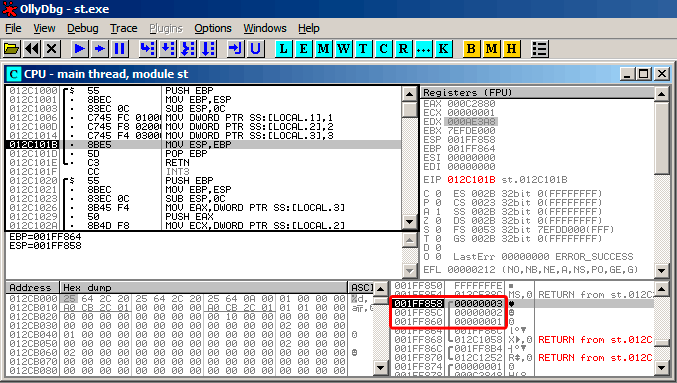
\includegraphics[scale=\FigScale]{patterns/02_stack/08_noise/olly1.png}
\caption{\olly: \TT{f1()}}
\label{fig:stack_noise_olly1}
\end{figure}

\RU{Когда}\EN{When} \TT{f1()} \RU{заполняет переменные}\EN{writes to} $a$, $b$ \AndENRU $c$ 
\RU{они сохранаяются по адресу}\EN{variables, they are stored at the address} \TT{0x14F85C} 
\RU{итд}\EN{and so on}.

\clearpage
\RU{А когда исполняется}\EN{And when} \TT{f2()}\EN{ executed}:

\begin{figure}[H]
\centering
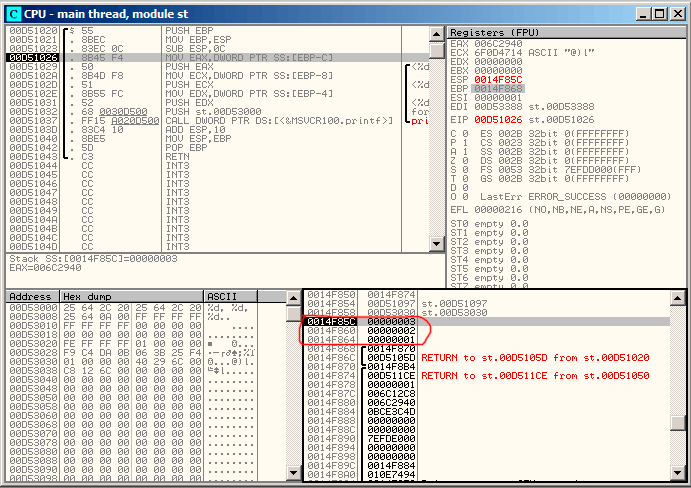
\includegraphics[scale=\FigScale]{patterns/02_stack/08_noise/olly2.png}
\caption{\olly: \TT{f2()}}
\label{fig:stack_noise_olly2}
\end{figure}

... $a$, $b$ \AndENRU $c$ \RU{в ф-ции}\EN{of} \TT{f2()} \RU{находятся по тем же адресам!}
\EN{are located at the same address!}
\RU{Пока никто не перезаписал их, так что они здесь в нетронутом виде.}
\EN{No one overwritten values yet, so they are still untouched here.}

\RU{Так что, для такой странной ситуации, несколько ф-ций должны исполняться друг за другом,
и \ac{SP} должен быть таким же при входе в ф-цию (т.е., у них должно быть равное кол-во
аргументов). Тогда, локальные переменные будут расположены в том же месте стека.}
\EN{So, for this weird situation, several functions should be called one after another and
\ac{SP} should be the same at each function entry (i.e., they should has same number
of arguments). Then, local variables will be located at the same point of stack.}

\RU{Подводя итоги, все значения в стеке (да и памяти вообще) это значения оставшиеся от 
исполнения предыдущих ф-ций}\EN{Summarizing, all values in stack (and memory cells at all) 
has values left there from previous function executions}.
\RU{Строго говоря, они не случайны, они скорее непредсказуемы}\EN{They are not 
random in strict sense, but rather has unpredictable values}.

\RU{А как иначе}\EN{How else}?
\RU{Вероятно, было бы возможным очищать части стека перед исполнением каждой ф-ции,
но это слишком много лишней (и ненужной) работы.}
\EN{Probably, it would be possible to clear stack portions before each function execution,
but that's too much extra (and needless) work.}

\fi
\ifdefined\IncludeExercises
\section{\Exercises}

\begin{itemize}
	\item \url{http://challenges.re/51}
	\item \url{http://challenges.re/52}
\end{itemize}


\fi

\chapter{\PrintfSeveralArgumentsSectionName}

\RU{Попробуем теперь немного расширить пример \IT{\HelloWorldSectionName}~(\ref{sec:helloworld}),
написав в теле функции \main:}
\EN{Now let's extend the \IT{\HelloWorldSectionName}~(\ref{sec:helloworld}) example, replacing \printf in
the \main function body by this:}

\lstinputlisting[label=hw_c]{patterns/03_printf/1.c}

% sections
\section{x86: \RU{3 аргумента}\EN{3 arguments}}

\subsection{MSVC}

\RU{Компилируем при помощи MSVC 2010 Express, и в итоге получим:}
\EN{Let's compile it by MSVC 2010 Express and we got:}

\begin{lstlisting}
$SG3830	DB	'a=%d; b=%d; c=%d', 00H

...

	push	3
	push	2
	push	1
	push	OFFSET $SG3830
	call	_printf
	add	esp, 16					; 00000010H
\end{lstlisting}

\RU{Все почти то же, за исключением того, что теперь видно, что аргументы для \printf заталкиваются в стек в обратном порядке: самый первый аргумент заталкивается последним.}
\EN{Almost the same, but now we can see the \printf arguments are pushed onto the stack in reverse order. The first argument is pushed last.}

\RU{Кстати, вспомним что переменные типа \Tint в 32-битной системе, как известно, имеет ширину 32 бита, это 4 байта}
\EN{By the way, variables of \Tint type in 32-bit environment have 32-bit width, that is 4 bytes}.

\RU{Итак, у нас всего 4 аргумента. $4*4 = 16$ ~--- именно 16 байт занимают в стеке указатель на строку плюс еще 3 числа типа \Tint.}
\EN{So, we have here 4 arguments. $4*4 = 16$~---they occupy exactly 16 bytes in the stack: a 32-bit pointer to a string and 3 numbers of type \Tint.}

\index{x86!\Instructions!ADD}
\index{x86!\Registers!ESP}
\index{cdecl}
\RU{Когда при помощи инструкции \TT{``ADD ESP, X''} корректируется \glslink{stack pointer}{указатель стека} \ESP 
после вызова какой-либо функции, зачастую можно сделать вывод о том, сколько аргументов 
у вызываемой функции было, разделив X на 4.}
\EN{When the \gls{stack pointer} (\ESP register) is changed back by the \TT{``ADD ESP, X''}
instruction after a function 
call, often, the number of function arguments can be deduced here: just divide X by 4.}

\RU{Конечно, это относится только к cdecl-методу передачи аргументов через стек.}
\EN{Of course, this is specific to the \IT{cdecl} calling convention.}

\RU{См. также в соответствующем разделе о способах передачи аргументов через стек}
\EN{See also the section about calling conventions}~(\ref{sec:callingconventions}).

\RU{Иногда бывает так, что подряд идут несколько вызовов разных функций, 
но стек корректируется только один раз, после последнего вызова:}
\EN{It is also possible for the compiler to merge several \TT{``ADD ESP, X''} instructions into one, after the last call:}

\begin{lstlisting}
push a1
push a2
call ...
...
push a1
call ...
...
push a1
push a2
push a3
call ...
add esp, 24
\end{lstlisting}

\subsection{MSVC \AndENRU \olly}
\index{\olly}

\RU{Попробуем этот же пример в}\EN{Now let's try to load this example in} \olly.
\RU{Это один из наиболее популярных win32-отладчиков user-режима}\EN{It is one of the most 
popular user-land win32 debugger}.
\RU{Мы можем компилировать наш пример в}\EN{We can try to compile our example in} MSVC 2012 
\RU{с опцией}\EN{with} \TT{/MD} \RU{что означает, линковать с библиотекой}\EN{option, meaning, to link 
against} \TT{MSVCR*.DLL},
\RU{чтобы импортируемые ф-ции были хорошо видны в отладчике}\EN{so we will able to see imported 
functions clearly in the debugger}.

\RU{Затем загружаем исполняемый файл в}\EN{Then load executable in} \olly.
\RU{Самый первый брякпойнт в}\EN{The very first breakpoint is in} \TT{ntdll.dll}, \RU{нажмите}\EN{press} 
F9 (\RU{запустить}\EN{run}).
\RU{Второй брякпойнт в}\EN{The second breakpoint is in} \ac{CRT}-\RU{коде}\EN{code}.
\RU{Теперь мы должны найти ф-цию}\EN{Now we should find the} \main\EN{ function}.

\RU{Найдите этот код скроллируя окно кода до самого верха (MSVC располагает ф-цию \main в самом начале
секции кода)}\EN{Find this code by scrolling the code to the very top (MSVC allocates \main function at
the very beginning of the code section)}: 
\figref{fig:printf3_olly_1}.\\
\\
\RU{Кликните на инструкции}\EN{Click on the} \TT{PUSH EBP}\RU{, нажмите}\EN{ instruction, press} F2 
(\RU{установка брякпойнта}\EN{set breakpoint}) \RU{и нажмите}\EN{and press} F9 (\RU{запустить}\EN{run}).
\RU{Нам нужно произвести все эти манипуляции, чтобы пропустить \ac{CRT}-код, потому что нам он пока
не интересен}\EN{We need to do these manipulations in order to skip \ac{CRT}-code, because, we aren't really
interested in it, yet}.\\
\\
\RU{Нажмите}\EN{Press} F8 (\stepover) 6 \RU{раз, т.е., пропустить
6 инструкций}\EN{times, i.e., skip 6 instructions}: \figref{fig:printf3_olly_2}.\\
\\
\RU{Теперь}\EN{Now the} \ac{PC} \RU{указывает на инструкцию}\EN{points to the}
\TT{CALL printf}\EN{ instruction}.
\olly, \RU{как и другие отладчики, подсвечивает регистры со значениями, которые изменились}
\EN{like other debuggers, highlights value of registers which were changed}.
\RU{Так что, каждый раз, когда мы нажимаем}\EN{So each time you press F8}, \EIP 
\RU{изменяется и его значение подсвечивается красным}\EN{ changes and its value looks red}.
\ESP \RU{также меняется, потому что значения заталкиваются в стек}\EN{changes as well, 
because values are pushed into the stack}.\\
\\
\RU{Где находятся эти значения в стеке}\EN{Where are the values in the stack}?
\RU{Посмотрите на правое/нижнее окно в отладчике}\EN{Take a look at the right/bottom window of debugger}:

\begin{figure}[H]
\centering
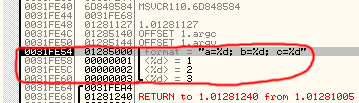
\includegraphics[scale=0.66]{patterns/03_printf/olly3_stack.png}
\caption{\olly: \RU{стек, после того как значения там сохранены}\EN{stack after values pushed}
(\RU{я сделал здесь округлую красную пометку в графическом редакторе}\EN{I made the round red mark 
here in a graphics editor})}
\end{figure}

\RU{Так что здесь видно 3 столбца: адрес в стеке, значение в стеке и еще дополнительный комментарий
от \olly}\EN{So we can see 3 columns there: address in the stack, 
value in the stack and some additional \olly comments}. 
\olly \RU{понимает}\EN{understands} \printf\RU{-строки}\EN{-like strings}, 
\RU{так что он показывает здесь и строку и 3 значения \IT{привязанных} к ней}\EN{so it reports the 
string here and 3 values \IT{attached} to it}.

\RU{Можно кликнуть правой кнопкой мыши на строке формата, кликнуть на ``Follow in dump''
и строка формата появится в окне слева внизу, где всегда виден какой-либо участок памяти}
\EN{It is possible to right-click on the format string, click on ``Follow in dump'',
and the format string will appear in the window at the left-bottom part, where some memory part
is always seen}.
\RU{Эти значения в памяти можно редактировать}\EN{These memory values can be edited}.
\RU{Можно изменить саму строку формата, и тогда результат работы нашего примера будет другой}
\EN{It is possible to change the format string, and then the result of our example will be different}.
\RU{В данном случае, пользы от этого немного, но для упражнения это полезно,
чтобы начать чувствовать как тут всё работает}\EN{It is probably not very useful now, but it's a very
good idea for doing it as an exercise, to get a feeling of how everything works here}.

\RU{Нажмите}\EN{Press} F8 (\stepover).

\RU{В консоли мы видим вывод}\EN{In the console we'll see the output}:

\begin{figure}[H]
\centering
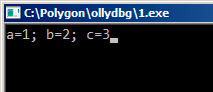
\includegraphics[scale=0.66]{patterns/03_printf/olly3_console.png}
\caption{\RU{Ф-ция }\printf \RU{исполнилась}\EN{function executed}}
\end{figure}

\RU{Посмотрим, как изменились регистры и состояние стека}\EN{Let's see how registers and stack state 
are changed}: \figref{fig:printf3_olly_3}.

\RU{Регистр }\EAX \RU{теперь содержит}\EN{register now contains} \TT{0xD} (13).
That's correct, since \printf returns the number of characters printed. The
\RU{Значение }\EIP \RU{изменилось: действительно, теперь здесь адрес инструкции после}
\EN{value is changed: indeed, now there is the address of the instruction after} \TT{CALL printf}.
\RU{Значения регистров }\ECX \AndENRU \EDX \RU{также изменились}\EN{values are changed as well}.
\RU{Очевидно, внутренности ф-ции \printf используют их для каких-то своих нужд}\EN{Apparently, 
\printf function's hidden machinery used them for its own needs}.

\RU{Очень важный момент в том что значение \ESP не изменилось. И аргменты-значения в стеке также!}
\EN{A very important fact is that neither the \ESP value, nor the stack state is changed!}
\RU{Мы ясно видим здесь и строку формата и соответствующие ей 3 значения, они все еще здесь.}
\EN{We clearly see that the format string and corresponding 3 values are still there.}
\RU{Действительно, по соглашению вызовов \IT{cdecl}, вызываемая ф-ция не возвращает \ESP назад.}
\EN{Indeed, that's the \IT{cdecl} calling convention: \gls{callee} doesn't return \ESP back to its previous value.}
\RU{Это должна делать вызывающая ф-ция}\EN{It's the \gls{caller}'s duty to do so}.

\RU{Нажмите}\EN{Press} F8 \RU{снова, чтобы исполнилась инструкция}\EN{again to execute} 
\TT{ADD ESP, 10}\EN{ instruction}: \figref{fig:printf3_olly_4}.

\ESP \RU{изменился, но значения все еще в стеке}\EN{is changed, but the values are still in the stack}!
\RU{Конечно, никому не нужно заполнять эти значения нулями или что-то в этом роде}\EN{Yes, 
of course; no one needs to fill these values by zero or something like that}.
\RU{Потому что всё что выше указателя стека}\EN{Because everything above stack pointer} (\ac{SP}) 
\RU{это}\EN{is} \IT{\RU{шум}\EN{noise}} \OrENRU \IT{\RU{мусор}\EN{garbage}}, \RU{это всё не имеет
особой ценности}\EN{and has no meaning at all}.
\RU{Было бы очень затратно по времени очищать ненужные элементы стека, к тому же, никому это и не 
нужно}\EN{It would be time consuming to clear unused stack entries anyways, and no one really needs to}.

\begin{figure}[H]
\centering
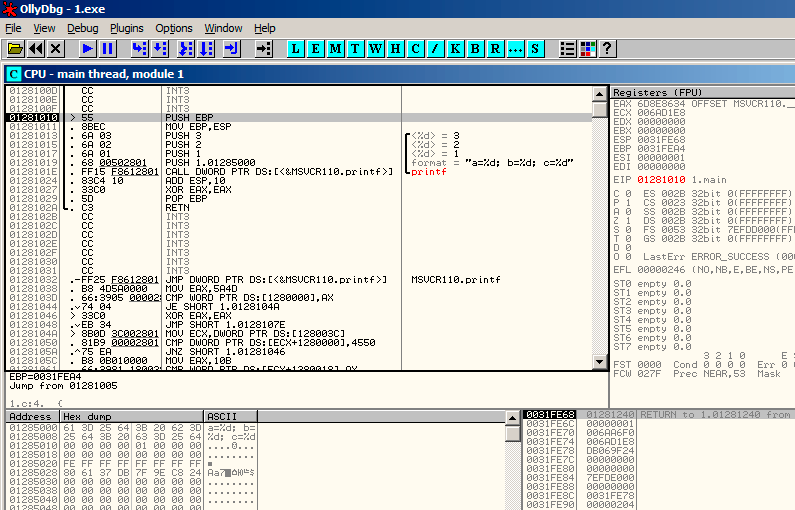
\includegraphics[scale=\FigScale]{patterns/03_printf/olly3_1.png}
\caption{\olly: \RU{самое начало ф-ции}\EN{the very start of the} \main\EN{ function}}
\label{fig:printf3_olly_1}
\end{figure}

\begin{figure}[H]
\centering
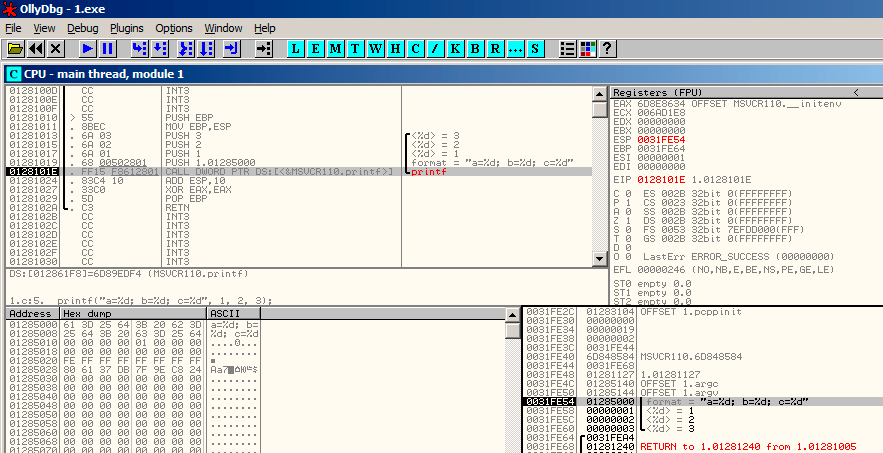
\includegraphics[scale=\FigScale]{patterns/03_printf/olly3_2.png}
\caption{\olly: \RU{перед исполнением}\EN{before} \printf\EN{ execution}}
\label{fig:printf3_olly_2}
\end{figure}

\begin{figure}[H]
\centering
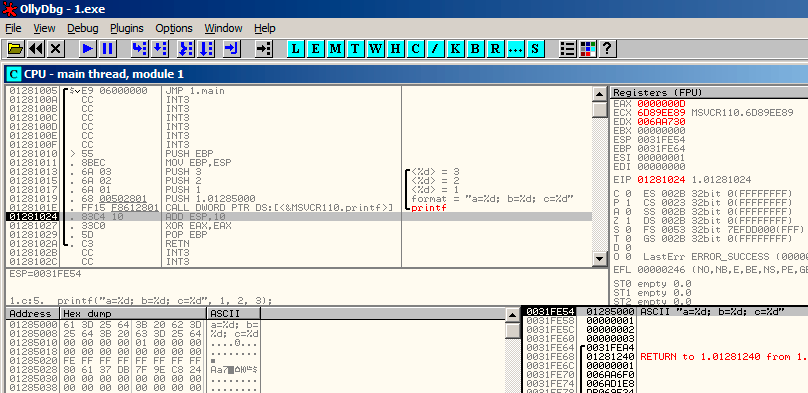
\includegraphics[scale=\FigScale]{patterns/03_printf/olly3_3.png}
\caption{\olly: \RU{после исполнения}\EN{after} \printf\EN{ execution}}
\label{fig:printf3_olly_3}
\end{figure}

\begin{figure}[H]
\centering
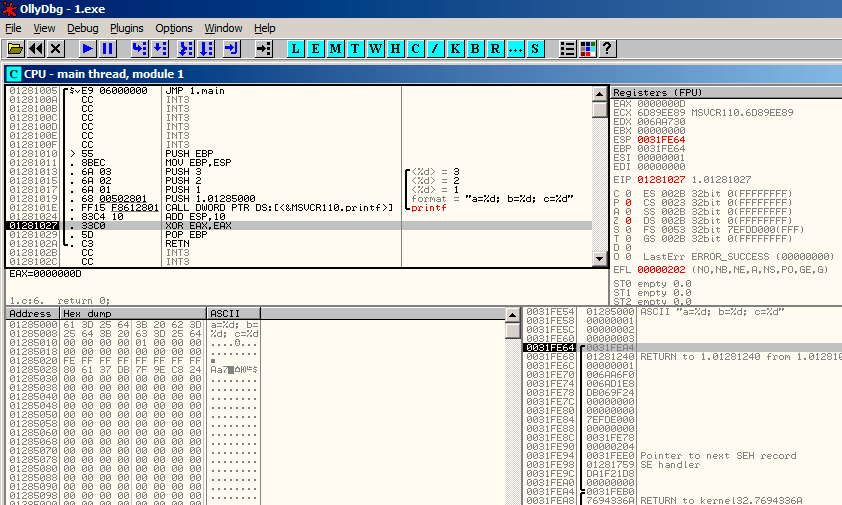
\includegraphics[scale=\FigScale]{patterns/03_printf/olly3_4.png}
\caption{\olly: \RU{после исполнения инструкции}\EN{after} \TT{ADD ESP, 10}\EN{ instruction execution}}
\label{fig:printf3_olly_4}
\end{figure}

\subsection{GCC}

\RU{Скомпилируем то же самое в Linux при помощи GCC 4.4.1 и посмотрим в \IDA что вышло:}
\EN{Now let's compile the same program in Linux using GCC 4.4.1 and take a look in \IDA what we got:}

\begin{lstlisting}
main            proc near

var_10          = dword ptr -10h
var_C           = dword ptr -0Ch
var_8           = dword ptr -8
var_4           = dword ptr -4

                push    ebp
                mov     ebp, esp
                and     esp, 0FFFFFFF0h
                sub     esp, 10h
                mov     eax, offset aADBDCD ; "a=%d; b=%d; c=%d"
                mov     [esp+10h+var_4], 3
                mov     [esp+10h+var_8], 2
                mov     [esp+10h+var_C], 1
                mov     [esp+10h+var_10], eax
                call    _printf
                mov     eax, 0
                leave
                retn
main            endp
\end{lstlisting}

\RU{Можно сказать, что этот короткий код, созданный GCC, отличается от кода MSVC только способом помещения 
значений в стек.
Здесь GCC снова работает со стеком напрямую без \PUSH/\POP.}
\EN{It can be said that the difference between code from MSVC and code from GCC is only in the method of placing arguments on the stack.
Here GCC is working directly with the stack without \PUSH/\POP.}

\subsection{GCC \AndENRU GDB}
\index{GDB}

\RU{Попробуем также этот пример и в \ac{GDB} в Linux}\EN{Let's try this example also in \ac{GDB} in Linux}.

\TT{-g} \RU{означает генерировать отладочную информацию в выходном исполняемом файле}\EN{mean produce 
debug information into executable file}.

\begin{lstlisting}
$ gcc 1.c -g -o 1
\end{lstlisting}

\begin{lstlisting}
$ gdb 1
GNU gdb (GDB) 7.6.1-ubuntu
Copyright (C) 2013 Free Software Foundation, Inc.
License GPLv3+: GNU GPL version 3 or later <http://gnu.org/licenses/gpl.html>
This is free software: you are free to change and redistribute it.
There is NO WARRANTY, to the extent permitted by law.  Type "show copying"
and "show warranty" for details.
This GDB was configured as "i686-linux-gnu".
For bug reporting instructions, please see:
<http://www.gnu.org/software/gdb/bugs/>...
Reading symbols from /home/dennis/polygon/1...done.
\end{lstlisting}

\begin{lstlisting}[caption=\RU{установим брякпойнт на}\EN{let's set breakpoint on} \printf]
(gdb) b printf
Breakpoint 1 at 0x80482f0
\end{lstlisting}

\RU{Запукаем}\EN{Run}.
\RU{Здесь у нас нет исходного кода ф-ции}\EN{There are no} \printf 
\RU{так что \ac{GDB} не может показать его исходный код, но могла бы}\EN{function source code here, 
so \ac{GDB} can't show its source, but may do so}.

\begin{lstlisting}
(gdb) run
Starting program: /home/dennis/polygon/1 

Breakpoint 1, __printf (format=0x80484f0 "a=%d; b=%d; c=%d") at printf.c:29
29	printf.c: No such file or directory.
\end{lstlisting}

\RU{Выдать 10 элементов стека. Левый столбец это адрес в стеке.}
\EN{Print 10 stack elements. The left column is an address in stack.}

\begin{lstlisting}
(gdb) x/10w $esp
0xbffff11c:	0x0804844a	0x080484f0	0x00000001	0x00000002
0xbffff12c:	0x00000003	0x08048460	0x00000000	0x00000000
0xbffff13c:	0xb7e29905	0x00000001
\end{lstlisting}

\RU{Самый первый элемент это}\EN{The very first element is the} \ac{RA} (\TT{0x0804844a}).
\RU{Мы можем удостовериться в этом, дизассемблируя память по этому адресу}\EN{We can make sure 
by disassembling the memory at this address}:

\begin{lstlisting}
(gdb) x/5i 0x0804844a
   0x804844a <main+45>:	mov    $0x0,%eax
   0x804844f <main+50>:	leave  
   0x8048450 <main+51>:	ret    
   0x8048451:	xchg   %ax,%ax
   0x8048453:	xchg   %ax,%ax
\end{lstlisting}

\RU{Две инструкции}\EN{Two} \TT{XCHG} 
\RU{это, вероятно, какой-то случайный мусор, который мы пока что можем игнорировать}
\EN{instructions, apparently, is some random garbage, which we can ignore so far}.

\RU{Второй элемент}\EN{The second element} (\TT{0x080484f0}) \RU{это адрес
строки формата}\EN{is an address of format string}:

\begin{lstlisting}
(gdb) x/s 0x080484f0
0x80484f0:	"a=%d; b=%d; c=%d"
\end{lstlisting}

\RU{Остальные 3 элемента}\EN{Other 3 elements} (1, 2, 3) \RU{это аргументы ф-ции}\EN{are} 
\printf\EN{ arguments}.
\RU{Остальные элементы это может быть и мусор в стеке, но могут быть и значения
от других ф-ций, их локальные переменные, итд}\EN{Other elements may be just ``garbage'' present in stack,
but also may be values from other functions, their local variables, etc}.
\RU{Пока что мы можем игнорировать их}\EN{We can ignore it for now}.

\RU{Исполняем}\EN{Execute} ``finish''. 
\RU{Это значит, исполнять до конца ф-ции}\EN{This mean, execute till function end}. 
\RU{Здесь это означает: исполнять до завершения}\EN{Here it means: execute till the finish of} \printf.

\begin{lstlisting}
(gdb) finish
Run till exit from #0  __printf (format=0x80484f0 "a=%d; b=%d; c=%d") at printf.c:29
main () at 1.c:6
6		return 0;
Value returned is $2 = 13
\end{lstlisting}

\ac{GDB} \RU{показывает, что вернула}\EN{shows what} \printf \RU{в}\EN{returned in} \EAX (13).
\RU{Это, так же как и в примере с \olly, количество напечатанных символов}
\EN{This is number of characters printed, just like in the example with \olly}.

\RU{А еще мы видим}\EN{We also see} ``return 0;'' \RU{и что это выражение находится в файле 
\TT{1.c} в строке 6}\EN{and the information that this expression is in the \TT{1.c} file at the line 6}.
\RU{Действительно, файл \TT{1.c} лежит в текущем директории и \ac{GDB} находит там эту строку}
\EN{Indeed, the \TT{1.c} file is located in the current directory, and \ac{GDB} finds the string there}.
\RU{Как \ac{GDB} знает, какая строка Си-кода сейчас исполняется}\EN{How does \ac{GDB} know which C-code line
is being executed now}?
\RU{Это связано с тем фактом, что компилятор, генерируя отладочную информацию,
также сохраняет информацию о 
соответствии строк в исходном коде и адресов инструкций}\EN{This is due to the fact that the compiler,
while generating debugging information, also saves a table of relations between source code line
numbers and instruction addresses}.
GDB \RU{это всё-таки отладчик уровня исходных текстов}\EN{is a source-level debugger, after all}.

\RU{Посмотрим регистры}\EN{Let's examine registers}.
13 \InENRU \EAX:

\begin{lstlisting}
(gdb) info registers
eax            0xd	13
ecx            0x0	0
edx            0x0	0
ebx            0xb7fc0000	-1208221696
esp            0xbffff120	0xbffff120
ebp            0xbffff138	0xbffff138
esi            0x0	0
edi            0x0	0
eip            0x804844a	0x804844a <main+45>
...
\end{lstlisting}

\RU{Попробуем дизассемблировать текущие инструкции}\EN{Let's disassemble the current instructions}.
\RU{Стрелка указывает на инструкцию, которая будет исполнена следующей}\EN{The arrow points to the 
instruction to be executed next}.

\begin{lstlisting}
(gdb) disas
Dump of assembler code for function main:
   0x0804841d <+0>:	push   %ebp
   0x0804841e <+1>:	mov    %esp,%ebp
   0x08048420 <+3>:	and    $0xfffffff0,%esp
   0x08048423 <+6>:	sub    $0x10,%esp
   0x08048426 <+9>:	movl   $0x3,0xc(%esp)
   0x0804842e <+17>:	movl   $0x2,0x8(%esp)
   0x08048436 <+25>:	movl   $0x1,0x4(%esp)
   0x0804843e <+33>:	movl   $0x80484f0,(%esp)
   0x08048445 <+40>:	call   0x80482f0 <printf@plt>
=> 0x0804844a <+45>:	mov    $0x0,%eax
   0x0804844f <+50>:	leave  
   0x08048450 <+51>:	ret    
End of assembler dump.
\end{lstlisting}

\ac{GDB} \RU{показывает дизассемблированный листинг в формате}\EN{shows disassembly in} AT\&T 
\RU{по умолчанию}\EN{syntax by default}.
\RU{Но можно также переключиться в формат Intel}\EN{It's possible to switch to Intel syntax}:

\begin{lstlisting}
(gdb) set disassembly-flavor intel
(gdb) disas
Dump of assembler code for function main:
   0x0804841d <+0>:	push   ebp
   0x0804841e <+1>:	mov    ebp,esp
   0x08048420 <+3>:	and    esp,0xfffffff0
   0x08048423 <+6>:	sub    esp,0x10
   0x08048426 <+9>:	mov    DWORD PTR [esp+0xc],0x3
   0x0804842e <+17>:	mov    DWORD PTR [esp+0x8],0x2
   0x08048436 <+25>:	mov    DWORD PTR [esp+0x4],0x1
   0x0804843e <+33>:	mov    DWORD PTR [esp],0x80484f0
   0x08048445 <+40>:	call   0x80482f0 <printf@plt>
=> 0x0804844a <+45>:	mov    eax,0x0
   0x0804844f <+50>:	leave  
   0x08048450 <+51>:	ret    
End of assembler dump.
\end{lstlisting}

\RU{Исполняем следующую инструкцию}\EN{Execute next instruction}.
\ac{GDB} \RU{покажет закрывающуюся скобку, означая, что это конец блока в ф-ции}\EN{shows ending bracket, 
meaning, this ends the block of the function}.

\begin{lstlisting}
(gdb) step
7	};
\end{lstlisting}

\RU{Посмотрим регистры после исполнения инструкции}\EN{Let's see the registers after the} 
\TT{MOV EAX, 0}\EN{ instruction execution}.
\EAX \RU{здесь уже действительно ноль}\EN{here is zero indeed}.

\begin{lstlisting}
(gdb) info registers
eax            0x0	0
ecx            0x0	0
edx            0x0	0
ebx            0xb7fc0000	-1208221696
esp            0xbffff120	0xbffff120
ebp            0xbffff138	0xbffff138
esi            0x0	0
edi            0x0	0
eip            0x804844f	0x804844f <main+50>
...
\end{lstlisting}

\section{x64: \RU{8 аргументов}\EN{8 arguments}}

\index{x86-64}
\label{example_printf8_x64}
\RU{Для того, чтобы посмотреть, как остальные аргументы будут передаваться через стек, 
изменим пример еще раз, 
увеличив количество передаваемых аргументов до 9 (строка формата \printf и 8 переменных типа \Tint)}
\EN{To see how other arguments will be passed via the stack, let's change our example again by increasing the number of arguments
to be passed to 9 (\printf format string + 8 \Tint variables)}:

\lstinputlisting{patterns/03_printf/2.c}

\subsection{MSVC}

\RU{Как уже было сказано раннее, первые 4 аргумента в Win64 передаются в регистрах}
\EN{As we saw before, the first 4 arguments are passed in the} \RCX, \RDX, \Reg{8}, \Reg{9}
\RU{, а остальные --- через стек}\EN{ registers in Win64, while all the rest---via the stack}.
\RU{Здесь мы это и видим}\EN{That is what we see here}.
\RU{Впрочем, инструкция \PUSH не используется, вместо нее, при помощи \MOV, значения сразу записываются в стек}
\EN{However, the \MOV instruction, instead of \PUSH, is used for preparing the stack, so the values are written
to the stack in a straightforward manner}.

\lstinputlisting[caption=MSVC 2012 x64]{patterns/03_printf/2_MSVC_x64.asm}

\RU{Наблюдательный читатель может спросить, почему для значений типа \Tint отводится 8 байт,
ведь нужно только 4?}
\EN{Observant reader may ask, what 8 bytes are allocated for \Tint values, while 4 is enough?}
\RU{Да, это нужно запомнить: для значений всех типов более коротких чем 64-бита, отводится 8 байт.}
\EN{Yes, this should be memorized: 8 bytes are allocated for any data type shorter than 64 bits.}
\RU{Это сделано для удобства: так всегда легко расчитать адрес того или иного аргумента.}
\EN{It's done for convenience: it's always easy to calculate address of this or that argument.}
\RU{К тому же, все они расположены по выровненным адресам в памяти.}
\EN{Besides, all they are located at aligned memory addresses.}
% also for local variables?
\RU{В 32-битных средах точно также: для всех типов резервируется 4 байта в стеке.}
\EN{The same story in 32-bit environments: 4 bytes are reserved for all data types.}

\subsection{GCC}

\RU{В *NIX-системах для x86-64 ситуация похожая, вот только первые 6 аргументов передаются через}
\EN{In *NIX OS-es, it's the same story for x86-64, except that the first 6 arguments are passed in the} \RDI, \RSI,
\RDX, \RCX, \Reg{8}, \Reg{9}\EN{ registers}.
\RU{Остальные --- через стек}\EN{All the rest---via the stack}.
\RU{GCC генерирует код записывающий указатель на строку в \EDI вместо \RDI --- 
это мы уже рассмотрели чуть раньше}\EN{GCC generates the code writing string pointer into \EDI instead if \RDI{}---we
saw this thing before}: \ref{hw_EDI_instead_of_RDI}.

\RU{Почему перед вызовом \printf очищается регистр \EAX, мы уже рассмотрели раннее}
\EN{We also saw before the \EAX register being cleared before a \printf call}: \ref{SysVABI_input_EAX}.

\lstinputlisting[caption=\Optimizing GCC 4.4.6 x64]{patterns/03_printf/2_GCC_x64_\LANG.s}

\ifdefined\IncludeGDB
\subsection{GCC + GDB}
\index{GDB}

\RU{Попробуем этот пример в}\EN{Let's try this example in} \ac{GDB}.

\begin{lstlisting}
$ gcc -g 2.c -o 2
\end{lstlisting}

\begin{lstlisting}
$ gdb 2
GNU gdb (GDB) 7.6.1-ubuntu
Copyright (C) 2013 Free Software Foundation, Inc.
License GPLv3+: GNU GPL version 3 or later <http://gnu.org/licenses/gpl.html>
This is free software: you are free to change and redistribute it.
There is NO WARRANTY, to the extent permitted by law.  Type "show copying"
and "show warranty" for details.
This GDB was configured as "x86_64-linux-gnu".
For bug reporting instructions, please see:
<http://www.gnu.org/software/gdb/bugs/>...
Reading symbols from /home/dennis/polygon/2...done.
\end{lstlisting}

\begin{lstlisting}[caption=\RU{ставим брякпойнт на \printf{,} запускаем}\EN{let's set the breakpoint to \printf{,} and run}]
(gdb) b printf
Breakpoint 1 at 0x400410
(gdb) run
Starting program: /home/dennis/polygon/2 

Breakpoint 1, __printf (format=0x400628 "a=%d; b=%d; c=%d; d=%d; e=%d; f=%d; g=%d; h=%d\n") at printf.c:29
29	printf.c: No such file or directory.
\end{lstlisting}

\RU{В регистрах}\EN{Registers} \RSI/\RDX/\RCX/\Reg{8}/\Reg{9} 
\RU{всё предсказуемо}\EN{has the values which are should be there}.
\RU{А }\RIP \RU{содержит адрес самой первой инструкции ф-ции}\EN{has an address of the very first instruction
of the} \printf\EN{ function}.

\begin{lstlisting}
(gdb) info registers
rax            0x0	0
rbx            0x0	0
rcx            0x3	3
rdx            0x2	2
rsi            0x1	1
rdi            0x400628	4195880
rbp            0x7fffffffdf60	0x7fffffffdf60
rsp            0x7fffffffdf38	0x7fffffffdf38
r8             0x4	4
r9             0x5	5
r10            0x7fffffffdce0	140737488346336
r11            0x7ffff7a65f60	140737348263776
r12            0x400440	4195392
r13            0x7fffffffe040	140737488347200
r14            0x0	0
r15            0x0	0
rip            0x7ffff7a65f60	0x7ffff7a65f60 <__printf>
...
\end{lstlisting}

\begin{lstlisting}[caption=\RU{смотрим на строку формата}\EN{let's inspect the format string}]
(gdb) x/s $rdi
0x400628:	"a=%d; b=%d; c=%d; d=%d; e=%d; f=%d; g=%d; h=%d\n"
\end{lstlisting}

\RU{Дампим стек на этот раз с командой x/g}\EN{Let's dump the stack with the x/g command this time}\EMDASH{}g 
\RU{означает}\EN{means} \IT{giant words}, \RU{т.е., 64-битные слова}\EN{i.e., 64-bit words}.

\begin{lstlisting}
(gdb) x/10g $rsp
0x7fffffffdf38:	0x0000000000400576	0x0000000000000006
0x7fffffffdf48:	0x0000000000000007	0x00007fff00000008
0x7fffffffdf58:	0x0000000000000000	0x0000000000000000
0x7fffffffdf68:	0x00007ffff7a33de5	0x0000000000000000
0x7fffffffdf78:	0x00007fffffffe048	0x0000000100000000
\end{lstlisting}

\RU{Самый первый элемент стека, как и в прошлый раз, это}\EN{The very first stack element, 
just like in the previous case, is the} \ac{RA}.
\RU{Через стек также передаются 3 значения}\EN{3 values are also passed in stack}: 6, 7, 8.
\RU{Видно, что 8 передается с не очищенной старшей 32-битной частью}\EN{We also see that 8 is passed
with high 32-bits not cleared}: \TT{0x00007fff00000008}.
\RU{Это нормально, ведь передаются числа типа \Tint, а они 32-битные}\EN{That's OK, because the values have
\Tint type, which is 32-bit type}.
\RU{Так что в старшей части регистра или памяти стека остался ``случайный мусор''}\EN{So, the high register
or stack element part may contain ``random garbage''}.

\RU{\ac{GDB} показывает всю ф-цию \main, если попытаться посмотреть, куда возвратится управление после
исполнения \printf}\EN{If you take a look at where control flow will return after \printf execution,
\ac{GDB} will show the whole \main function}:

\begin{lstlisting}
(gdb) set disassembly-flavor intel
(gdb) disas 0x0000000000400576
Dump of assembler code for function main:
   0x000000000040052d <+0>:	push   rbp
   0x000000000040052e <+1>:	mov    rbp,rsp
   0x0000000000400531 <+4>:	sub    rsp,0x20
   0x0000000000400535 <+8>:	mov    DWORD PTR [rsp+0x10],0x8
   0x000000000040053d <+16>:	mov    DWORD PTR [rsp+0x8],0x7
   0x0000000000400545 <+24>:	mov    DWORD PTR [rsp],0x6
   0x000000000040054c <+31>:	mov    r9d,0x5
   0x0000000000400552 <+37>:	mov    r8d,0x4
   0x0000000000400558 <+43>:	mov    ecx,0x3
   0x000000000040055d <+48>:	mov    edx,0x2
   0x0000000000400562 <+53>:	mov    esi,0x1
   0x0000000000400567 <+58>:	mov    edi,0x400628
   0x000000000040056c <+63>:	mov    eax,0x0
   0x0000000000400571 <+68>:	call   0x400410 <printf@plt>
   0x0000000000400576 <+73>:	mov    eax,0x0
   0x000000000040057b <+78>:	leave  
   0x000000000040057c <+79>:	ret    
End of assembler dump.
\end{lstlisting}

\RU{Заканчиваем исполнение \printf, исполняем инструкцию обнуляющую \EAX, 
удостоверяемся что в регистре \EAX именно ноль}\EN{Let's finish executing \printf, execute the instruction
zeroing \EAX, and note that the \EAX register has a value of exactly zero}.
\RIP \RU{указывает сейчас на инструкцию}\EN{now points to the} \TT{LEAVE}\RU{, т.е., предпоследнюю в ф-ции \main}
\EN{ instruction, i.e., the penultimate one in the \main function}.

\begin{lstlisting}
(gdb) finish
Run till exit from #0  __printf (format=0x400628 "a=%d; b=%d; c=%d; d=%d; e=%d; f=%d; g=%d; h=%d\n") at printf.c:29
a=1; b=2; c=3; d=4; e=5; f=6; g=7; h=8
main () at 2.c:6
6		return 0;
Value returned is $1 = 39
(gdb) next
7	};
(gdb) info registers
rax            0x0	0
rbx            0x0	0
rcx            0x26	38
rdx            0x7ffff7dd59f0	140737351866864
rsi            0x7fffffd9	2147483609
rdi            0x0	0
rbp            0x7fffffffdf60	0x7fffffffdf60
rsp            0x7fffffffdf40	0x7fffffffdf40
r8             0x7ffff7dd26a0	140737351853728
r9             0x7ffff7a60134	140737348239668
r10            0x7fffffffd5b0	140737488344496
r11            0x7ffff7a95900	140737348458752
r12            0x400440	4195392
r13            0x7fffffffe040	140737488347200
r14            0x0	0
r15            0x0	0
rip            0x40057b	0x40057b <main+78>
...
\end{lstlisting}
\fi

\ifdefined\IncludeARM
\subsection{ARM: \RU{3 аргумента}\EN{3 arguments}}

\RU{В ARM традиционно принята такая схема передачи аргументов в функцию: 
4 первых аргумента через регистры \Reg{0}-\Reg{3}; а остальные~--- через стек}
\EN{ARM's traditional scheme for passing arguments (calling convention) behaves as follows:
the first 4 arguments are passed through the \Reg{0}-\Reg{3} registers; the remaining arguments via the stack}.
\RU{Это немного похоже на то, как аргументы передаются в}\EN{This resembles the arguments passing scheme in} 
fastcall~(\myref{fastcall}) \OrENRU win64~(\myref{sec:callingconventions_win64}).

\subsubsection{32-\RU{битный}\EN{bit} ARM}

\myparagraph{\NonOptimizingKeilVI (\ARMMode)}

\begin{lstlisting}[caption=\NonOptimizingKeilVI (\ARMMode)]
.text:00000000 main
.text:00000000 10 40 2D E9   STMFD   SP!, {R4,LR}
.text:00000004 03 30 A0 E3   MOV     R3, #3
.text:00000008 02 20 A0 E3   MOV     R2, #2
.text:0000000C 01 10 A0 E3   MOV     R1, #1
.text:00000010 08 00 8F E2   ADR     R0, aADBDCD     ; "a=%d; b=%d; c=%d"
.text:00000014 06 00 00 EB   BL      __2printf
.text:00000018 00 00 A0 E3   MOV     R0, #0          ; return 0
.text:0000001C 10 80 BD E8   LDMFD   SP!, {R4,PC}
\end{lstlisting}

\RU{Итак, первые 4 аргумента передаются через регистры \Reg{0}-\Reg{3}, по порядку: 
указатель на формат-строку для \printf
в \Reg{0}, затем 1 в \Reg{1}, 2 в \Reg{2} и 3 в \Reg{3}}
\EN{So, the first 4 arguments are passed via the \Reg{0}-\Reg{3} registers in this order:
a pointer to the \printf format string in 
\Reg{0}, then 1 in \Reg{1}, 2 in \Reg{2} and 3 in \Reg{3}}.

\RU{Инструкция на}\EN{The instruction at} \TT{0x18} \RU{записывает}\EN{writes} 0 \RU{в}\EN{to} \Reg{0}
\EMDASH{}\RU{это выражение в Си}\EN{this is} \IT{return 0}\EN{ C-statement}.

\RU{Пока что здесь нет ничего необычного}\EN{There is nothing unusual so far}.

\OptimizingKeilVI \RU{генерирует точно такой же код}\EN{generates the same code}.

\myparagraph{\OptimizingKeilVI (\ThumbMode)}

\begin{lstlisting}[caption=\OptimizingKeilVI (\ThumbMode)]
.text:00000000 main
.text:00000000 10 B5        PUSH    {R4,LR}
.text:00000002 03 23        MOVS    R3, #3
.text:00000004 02 22        MOVS    R2, #2
.text:00000006 01 21        MOVS    R1, #1
.text:00000008 02 A0        ADR     R0, aADBDCD     ; "a=%d; b=%d; c=%d"
.text:0000000A 00 F0 0D F8  BL      __2printf
.text:0000000E 00 20        MOVS    R0, #0
.text:00000010 10 BD        POP     {R4,PC}
\end{lstlisting}

\RU{Здесь нет особых отличий от неоптимизированного варианта для режима ARM}
\EN{There is no significant difference from the non-optimized code for ARM mode}.

\myparagraph{\OptimizingKeilVI (\ARMMode) + \RU{убираем}\EN{let's remove} return}
\label{ARM_B_to_printf}

\RU{Немного переделаем пример, убрав}\EN{Let's rework example slightly by removing} \IT{return 0}:

\begin{lstlisting}
#include <stdio.h>

void main()
{
	printf("a=%d; b=%d; c=%d", 1, 2, 3);
};
\end{lstlisting}

\RU{Результат получится необычным:}
\EN{The result is somewhat unusual:}

\begin{lstlisting}[caption=\OptimizingKeilVI (\ARMMode)]
.text:00000014 main
.text:00000014 03 30 A0 E3   MOV     R3, #3
.text:00000018 02 20 A0 E3   MOV     R2, #2
.text:0000001C 01 10 A0 E3   MOV     R1, #1
.text:00000020 1E 0E 8F E2   ADR     R0, aADBDCD     ; "a=%d; b=%d; c=%d\n"
.text:00000024 CB 18 00 EA   B       __2printf
\end{lstlisting}

\index{ARM!\Registers!Link Register}
\index{ARM!\Instructions!B}
\index{Function epilogue}
\RU{Это оптимизированная версия (\Othree) для режима ARM, и здесь мы видим последнюю инструкцию 
\TT{B} вместо привычной нам \TT{BL}}\EN{This is the optimized (\Othree) version for ARM mode and this time we see \TT{B} as the last instruction instead of the familiar \TT{BL}}.
\RU{Отличия между этой оптимизированной версией и предыдущей, скомпилированной без оптимизации, 
ещё и в том, 
что здесь нет пролога и эпилога функции (инструкций, сохраняющих состояние регистров \TT{\Reg{0}} и \ac{LR})}%
\EN{Another difference between this optimized version and the previous one (compiled without optimization)
is the lack of function prologue and epilogue (instructions preserving the \TT{\Reg{0}} and \ac{LR} registers values)}.
\index{x86!\Instructions!JMP}
\RU{Инструкция \TT{B} просто переходит на другой адрес, без манипуляций с регистром \ac{LR}, то есть
это аналог \JMP в x86}%
\EN{The \TT{B} instruction just jumps to another address, without any manipulation of the \ac{LR} register,
similar to \JMP in x86}.
\RU{Почему это работает нормально? Потому что этот код эквивалентен предыдущему.}
\EN{Why does it work? Because this code is, in fact, effectively equivalent to the previous.}
\RU{Основных причин две: 1) стек не модифицируется, как и \glslink{stack pointer}{указатель стека} \ac{SP}; 2) вызов функции \printf последний, 
после него ничего не происходит}\EN{There are two main reasons: 1) neither the stack nor \ac{SP} (the \gls{stack pointer}) is modified;
2) the call to \printf is the last instruction, so there is nothing going on afterwards}.
\RU{Функция \printf, отработав, просто возвращает управление по адресу, записанному в \ac{LR}.}
\EN{On completion, the \printf function simply returns the control to the address 
stored in \ac{LR}.}
\RU{Но в \ac{LR} находится адрес места, откуда была вызвана наша функция!
А следовательно, управление из \printf вернется сразу туда.}
\EN{Since the \ac{LR} currently stores the address of the point from where our function
was called then the control from \printf will be returned to that point.}
\RU{Значит нет нужды сохранять \ac{LR}, потому что нет нужны модифицировать \ac{LR}}%
\EN{Therefore we do not need to save \ac{LR} because we do not need to modify \ac{LR}}.
\RU{А нет нужды модифицировать \ac{LR}, потому что нет иных вызовов функций, кроме \printf, к тому же, после этого вызова не нужно ничего здесь больше делать}%
\EN{And we do not need to modify \ac{LR} because there are no other function calls except \printf. Furthermore,
after this call we do not to do anything else}!
\RU{Поэтому такая оптимизация возможна}\EN{That is the reason such optimization is possible}.

\RU{Эта оптимизация часто используется в функциях, где последнее выражение~--- это вызов другой функции.}
\EN{This optimization is often used in functions where the last statement is a call to another function.}

\RU{Ещё один похожий пример описан здесь}\EN{A similar example is presented here}:
\myref{jump_to_last_printf}.

\subsubsection{ARM64}

\myparagraph{\NonOptimizing GCC (Linaro) 4.9}

\lstinputlisting[caption=\NonOptimizing GCC (Linaro) 4.9]{patterns/03_printf/ARM/ARM3_O0.lst.\LANG}

\index{ARM!\Instructions!STP}
\RU{Итак, первая инструкция STP (Store Pair) сохраняет \ac{FP} (X29) и \ac{LR} (X30) в стеке.}
\EN{The first instruction STP (Store Pair) saves \ac{FP} (X29) and \ac{LR} (X30) in the stack.}
\RU{Вторая инструкция \TT{ADD X29, SP, 0} формирует стековый фрейм.}
\EN{The second \TT{ADD X29, SP, 0} instruction forms the stack frame.}
\RU{Это просто запись значения \ac{SP} в X29.}
\EN{It is just writing the value of \ac{SP} into X29.}

\index{ARM!\Instructions!ADRP/ADD pair}
\RU{Далее уже знакомая пара инструкций \TT{ADRP}/\ADD формирует указатель на строку.}
\EN{Next, we see the familiar \TT{ADRP}/\ADD instruction pair, which forms a pointer to the string.}

\RU{\TT{\%d} в формате \printf это 32-битный \Tint, так что 1, 2 и 3 заносятся в 32-битные части регистров.}
\EN{\TT{\%d} in \printf string format is a 32-bit \Tint, so the 1, 2 and 3 are loaded into 32-bit register parts.}

\Optimizing GCC (Linaro) 4.9 \RU{генерирует почти такой же код}\EN{generates the same code}.

\subsection{ARM: \RU{8 аргументов}\EN{8 arguments}}

\RU{Снова воспользуемся примером с 9-ю аргументами из предыдущей секции}\EN{Let's use again the example
with 9 arguments from the previous section}: \myref{example_printf8_x64}.

\lstinputlisting{patterns/03_printf/2.c}

\subsubsection{\OptimizingKeilVI: \ARMMode}

\begin{lstlisting}
.text:00000028             main
.text:00000028
.text:00000028             var_18 = -0x18
.text:00000028             var_14 = -0x14
.text:00000028             var_4  = -4
.text:00000028
.text:00000028 04 E0 2D E5  STR    LR, [SP,#var_4]!
.text:0000002C 14 D0 4D E2  SUB    SP, SP, #0x14
.text:00000030 08 30 A0 E3  MOV    R3, #8
.text:00000034 07 20 A0 E3  MOV    R2, #7
.text:00000038 06 10 A0 E3  MOV    R1, #6
.text:0000003C 05 00 A0 E3  MOV    R0, #5
.text:00000040 04 C0 8D E2  ADD    R12, SP, #0x18+var_14
.text:00000044 0F 00 8C E8  STMIA  R12, {R0-R3}
.text:00000048 04 00 A0 E3  MOV    R0, #4
.text:0000004C 00 00 8D E5  STR    R0, [SP,#0x18+var_18]
.text:00000050 03 30 A0 E3  MOV    R3, #3
.text:00000054 02 20 A0 E3  MOV    R2, #2
.text:00000058 01 10 A0 E3  MOV    R1, #1
.text:0000005C 6E 0F 8F E2  ADR    R0, aADBDCDDDEDFDGD ; "a=%d; b=%d; c=%d; d=%d; e=%d; f=%d; g=%"...
.text:00000060 BC 18 00 EB  BL     __2printf
.text:00000064 14 D0 8D E2  ADD    SP, SP, #0x14
.text:00000068 04 F0 9D E4  LDR    PC, [SP+4+var_4],#4
\end{lstlisting}

\RU{Этот код можно условно разделить на несколько частей}\EN{This code can be divided into several parts}:

\begin{itemize}
\index{Function prologue}
\item \RU{Пролог функции}\EN{Function prologue}:

\index{ARM!\Instructions!STR}
\RU{Самая первая инструкция}\EN{The very first} \TT{STR LR, [SP,\#var\_4]!} 
\RU{сохраняет в стеке \ac{LR}, ведь нам придется использовать этот регистр для вызова \printf}%
\EN{instruction saves \ac{LR} on the stack, because we are going to use this register for the \printf call}.
\RU{Восклицательный знак в конце означает}\EN{Exclamation mark at the end indicates} \IT{pre-index}.
\RU{Это значит, что в начале \ac{SP} должно быть
уменьшено на 4, затем по адресу в \ac{SP} должно быть записано значение \ac{LR}.}
\EN{This implies that \ac{SP} is to be decreased by 4 first, and then \ac{LR} will be saved at the address stored in \ac{SP}.}
\RU{Это аналог знакомой в x86 инструкции \PUSH}\EN{This is similar to \PUSH in x86}.
\RU{Читайте больше об этом}\EN{Read more about it at}: \myref{ARM_postindex_vs_preindex}.

\index{ARM!\Instructions!SUB}
\RU{Вторая инструкция}\EN{The second} \TT{SUB SP, SP, \#0x14}
\RU{уменьшает \glslink{stack pointer}{указатель стека} \ac{SP}, но, на самом деле, эта процедура нужна для выделения в локальном стеке места размером \TT{0x14} (20) байт.}
\EN{instruction decreases
\ac{SP} (the \gls{stack pointer}) in order to 
allocate \TT{0x14} (20) bytes on the stack.}
\RU{Действительно, нам нужно передать 5 32-битных значений через стек в \printf. Каждое значение занимает 4 байта, все вместе~--- $5*4=20$.}
\EN{Indeed, we need to pass 5 32-bit values via the stack to the \printf function, and each one occupies 4 bytes, which is exactly $5*4=20$.}
\RU{Остальные 4 32-битных значения будут переданы через регистры.}
\EN{The other 4 32-bit values are to be passed through registers.}

\item \RU{Передача 5, 6, 7 и 8 через стек}\EN{Passing 5, 6, 7 and 8 via the stack}:
\RU{они записываются в регистры \Reg{0}, \Reg{1}, \Reg{2} и \Reg{3} соответственно}%
\EN{they are stored in the \Reg{0}, \Reg{1}, \Reg{2} and \Reg{3} registers respectively}.
\RU{Затем инструкция}\EN{Then, the} \TT{ADD R12, SP, \#0x18+var\_14} 
\RU{записывает в регистр \TT{R12} адрес места в стеке, куда будут помещены эти 4 значения}%
\EN{instruction writes the stack address where these 4 variables are to be stored, into the \TT{R12} register}.
\index{IDA!var\_?}
\IT{var\_14}\RU{~--- это макрос ассемблера}\EN{ is an assembly macro}, \RU{равный}\EN{equal to} -0x14\RU{.}
\RU{Такие макросы создает \IDA, чтобы удобнее было показывать, как код обращается к стеку.}
\EN{, created by \IDA to conveniently display the code accessing the stack.}
\RU{Макросы \IT{var\_?}, создаваемые \IDA, отражают локальные переменные в стеке}\EN{The \IT{var\_?} macros generated
by \IDA reflect local variables in the stack.}
\RU{Так что в \TT{R12} будет записано \TT{SP+4}.}
\EN{So, \TT{SP+4} is to be stored into the \TT{R12} register.}
\index{ARM!\Instructions!STMIA}
\RU{Следующая инструкция}\EN{The next} \TT{STMIA R12, {R0-R3}} 
\RU{записывает содержимое регистров \Reg{0}-\Reg{3} по адресу в памяти, на который указывает \TT{R12}.}
\EN{instruction
writes registers \Reg{0}-\Reg{3} contents to the memory pointed by \TT{R12}.}
\RU{Инструкция }\TT{STMIA} \RU{означает}\EN{abbreviates} \IT{Store Multiple Increment After}. 
\IT{\q{Increment After}} 
\RU{означает, что \TT{R12} будет увеличиваться на 4 после записи каждого значения регистра.}
\EN{implies that \TT{R12} is to be increased by 4 after each register value is written.}

\item \RU{Передача 4 через стек}\EN{Passing 4 via the stack}:
\RU{4 записывается в \Reg{0}, затем инструкция}\EN{4 is stored in \Reg{0} and then
this value, with the help of the} \TT{STR R0, [SP,\#0x18+var\_18]} \RU{записывает его в стек}\EN{instruction is saved
on the stack}.
\IT{var\_18} \RU{равен}\EN{is} -0x18, \RU{смещение будет 0}\EN{so the offset is to be 0}, 
\RU{так что значение из регистра \Reg{0} (4) запишется туда, куда указывает \ac{SP}}%
\EN{thus the value from the \Reg{0} register (4) is to be written to the address written in \ac{SP}}.

\item \RU{Передача 1, 2 и 3 через регистры}\EN{Passing 1, 2 and 3 via registers}:

\RU{Значения для первых трех чисел (a, b, c) (1, 2, 3 соответственно) передаются в регистрах 
\Reg{1}, \Reg{2} и \Reg{3} перед самим вызовом \printf}%
\EN{The values of the first 3 numbers (a, b, c) (1, 2, 3 respectively) are passed through the 
\Reg{1}, \Reg{2} and \Reg{3}
registers right before the \printf call}, \RU{а остальные 5 значений передаются через стек, и вот как}\EN{and the other
5 values are passed via the stack}:

\item \RU{Вызов \printf}\EN{\printf call}.

\index{Function epilogue}
\item \RU{Эпилог функции}\EN{Function epilogue}:

\RU{Инструкция}\EN{The} \TT{ADD SP, SP, \#0x14} \RU{возвращает \ac{SP} на прежнее место, 
аннулируя таким образом всё, что было записано в стеке}%
\EN{instruction restores the \ac{SP} pointer back to its former value,
thus cleaning the stack}.
\RU{Конечно, то что было записано в стек, там пока и останется, но всё это будет многократно 
перезаписано во время исполнения последующих функций.}
\EN{Of course, what was stored on the stack will stay there, but it will all be
rewritten during the execution of subsequent functions.}

\index{ARM!\Instructions!LDR}
\RU{Инструкция}\EN{The} \TT{LDR PC, [SP+4+var\_4],\#4} \RU{загружает в \ac{PC} 
сохраненное значение \ac{LR} из стека, обеспечивая таким образом выход из функции.}
\EN{instruction loads the saved \ac{LR} value from the stack into the \ac{PC} register, 
thus causing the function to exit.}
\EN{There is no exclamation mark---indeed, \ac{PC} is loaded first from the address stored in \ac{SP} }
\RU{Здесь нет восклицательного знака~--- действительно, сначала \ac{PC} загружается из места,
куда указывает \ac{SP}}
($4+var\_4=4+(-4)=0$, \RU{так что эта инструкция аналогична}\EN{so this instruction is 
analogous to} \TT{LDR PC, [SP],\#4}), \RU{затем}\EN{and then} \ac{SP} \RU{увеличивается 
на}\EN{is increased by} 4.
\RU{Это называется}\EN{This is referred as} \IT{post-index}\footnote{\RU{Читайте больше об 
этом}\EN{Read more about it}: \myref{ARM_postindex_vs_preindex}.}.
\RU{Почему}\EN{Why does} \IDA \RU{показывает инструкцию именно так}\EN{display the instruction like that}?
\RU{Потому что она хочет показать разметку стека и тот факт, что}\EN{Because it wants to illustrate the stack layout and the fact that} \TT{var\_4} \RU{выделена в локальном стеке именно для сохраненного
значения}\EN{is allocated for saving the} \ac{LR}\EN{ value in the local stack}.
\RU{Эта инструкция в каком-то смысле аналогична}\EN{This instruction is somewhat 
similar to} \TT{POP PC} \InENRU x86\footnote{\EN{It is impossible to
set \TT{IP/EIP/RIP} value using \POP in x86, but anyway, you get the idea, I hope}\RU{В x86 
невозможно установить значение \TT{IP/EIP/RIP} используя \POP, но надеюсь, вы поняли, о чем я}.}.

\end{itemize}

\subsubsection{\OptimizingKeilVI: \ThumbMode}

\begin{lstlisting}
.text:0000001C             printf_main2
.text:0000001C
.text:0000001C             var_18 = -0x18
.text:0000001C             var_14 = -0x14
.text:0000001C             var_8  = -8
.text:0000001C
.text:0000001C 00 B5        PUSH    {LR}
.text:0000001E 08 23        MOVS    R3, #8
.text:00000020 85 B0        SUB     SP, SP, #0x14
.text:00000022 04 93        STR     R3, [SP,#0x18+var_8]
.text:00000024 07 22        MOVS    R2, #7
.text:00000026 06 21        MOVS    R1, #6
.text:00000028 05 20        MOVS    R0, #5
.text:0000002A 01 AB        ADD     R3, SP, #0x18+var_14
.text:0000002C 07 C3        STMIA   R3!, {R0-R2}
.text:0000002E 04 20        MOVS    R0, #4
.text:00000030 00 90        STR     R0, [SP,#0x18+var_18]
.text:00000032 03 23        MOVS    R3, #3
.text:00000034 02 22        MOVS    R2, #2
.text:00000036 01 21        MOVS    R1, #1
.text:00000038 A0 A0        ADR     R0, aADBDCDDDEDFDGD ; "a=%d; b=%d; c=%d; d=%d; e=%d; f=%d; g=%"...
.text:0000003A 06 F0 D9 F8  BL      __2printf
.text:0000003E
.text:0000003E             loc_3E   ; CODE XREF: example13_f+16
.text:0000003E 05 B0        ADD     SP, SP, #0x14
.text:00000040 00 BD        POP     {PC}
\end{lstlisting}

\RU{Это почти то же самое что и в предыдущем примере, только код для Thumb и значения помещаются в 
стек немного иначе: сначала 8 за первый раз, затем 5, 6, 7 за второй раз и 4 за третий раз}\EN{The output is almost 
like in
the previous example. However, this is Thumb code and the values are packed into stack differently: 
8 goes first, then 5, 6, 7, and 4 goes third}.

\subsubsection{\OptimizingXcodeIV: \ARMMode}

\begin{lstlisting}
__text:0000290C             _printf_main2
__text:0000290C
__text:0000290C             var_1C = -0x1C
__text:0000290C             var_C  = -0xC
__text:0000290C
__text:0000290C 80 40 2D E9   STMFD  SP!, {R7,LR}
__text:00002910 0D 70 A0 E1   MOV    R7, SP
__text:00002914 14 D0 4D E2   SUB    SP, SP, #0x14
__text:00002918 70 05 01 E3   MOV    R0, #0x1570
__text:0000291C 07 C0 A0 E3   MOV    R12, #7
__text:00002920 00 00 40 E3   MOVT   R0, #0
__text:00002924 04 20 A0 E3   MOV    R2, #4
__text:00002928 00 00 8F E0   ADD    R0, PC, R0
__text:0000292C 06 30 A0 E3   MOV    R3, #6
__text:00002930 05 10 A0 E3   MOV    R1, #5
__text:00002934 00 20 8D E5   STR    R2, [SP,#0x1C+var_1C]
__text:00002938 0A 10 8D E9   STMFA  SP, {R1,R3,R12}
__text:0000293C 08 90 A0 E3   MOV    R9, #8
__text:00002940 01 10 A0 E3   MOV    R1, #1
__text:00002944 02 20 A0 E3   MOV    R2, #2
__text:00002948 03 30 A0 E3   MOV    R3, #3
__text:0000294C 10 90 8D E5   STR    R9, [SP,#0x1C+var_C]
__text:00002950 A4 05 00 EB   BL     _printf
__text:00002954 07 D0 A0 E1   MOV    SP, R7
__text:00002958 80 80 BD E8   LDMFD  SP!, {R7,PC}
\end{lstlisting}

\index{ARM!\Instructions!STMFA}
\index{ARM!\Instructions!STMIB}
\RU{Почти то же самое, что мы уже видели, за исключением того, что}%
\EN{Almost the same as what we have already seen, with the
exception of} \TT{STMFA} (Store Multiple Full Ascending)%
\RU{~--- это синоним инструкции }\EN{ instruction, which is a synonym of}%
\TT{STMIB} (Store Multiple Increment Before)\EN{ instruction}. 
\RU{Эта инструкция увеличивает \ac{SP} и только затем записывает в память значение очередного регистра, 
но не наоборот}\EN{This
instruction increases the value in the \ac{SP} register and only then writes the next register value into the memory, rather than performing those two actions in the opposite order}.

\RU{Далее бросается в глаза то, что инструкции как будто бы расположены случайно}\EN{Another thing
that catches the eye is that the instructions are arranged seemingly random}.
\RU{Например, значение в регистре \Reg{0} подготавливается в трех местах, по адресам \TT{0x2918}, \TT{0x2920} 
и \TT{0x2928}, 
когда это можно было бы сделать в одном месте}\EN{For example, the value in the \Reg{0} register is manipulated in three
places, at addresses \TT{0x2918}, \TT{0x2920} and \TT{0x2928}, when it would be possible to do it in one point}.
\RU{Однако, у оптимизирующего компилятора могут быть свои доводы о том, как лучше составлять инструкции 
друг с другом для лучшей эффективности исполнения}%
\EN{However, the optimizing compiler may have its own reasons on how to order the instructions so to achieve higher efficiency during the execution}.
\RU{Процессор обычно пытается исполнять одновременно идущие друг за другом инструкции}%
\EN{Usually, the processor attempts to simultaneously execute instructions located side-by-side}.
\RU{К примеру, инструкции}\EN{For example, instructions like} \TT{MOVT R0, \#0} \AndENRU 
\TT{ADD R0, PC, R0} \RU{не могут быть исполнены одновременно, потому что обе инструкции модифицируют 
регистр \Reg{0}}\EN{cannot be executed simultaneously since they both modify the \Reg{0} register}. 
\RU{А вот инструкции}\EN{On the other hand,} \TT{MOVT R0, \#0} \AndENRU \TT{MOV R2, \#4} 
\RU{легко можно исполнить одновременно, 
потому что эффекты от их исполнения никак не конфликтуют друг с другом}\EN{instructions can be executed
simultaneously since the effects of their execution are not conflicting with each other}.
\RU{Вероятно, компилятор старается генерировать код именно таким образом там, где это возможно}%
\EN{Presumably, the compiler tries to generate code in such a manner (wherever it is possible)}.
 
\subsubsection{\OptimizingXcodeIV: \ThumbTwoMode}

\begin{lstlisting}
__text:00002BA0               _printf_main2
__text:00002BA0
__text:00002BA0               var_1C = -0x1C
__text:00002BA0               var_18 = -0x18
__text:00002BA0               var_C  = -0xC
__text:00002BA0
__text:00002BA0 80 B5          PUSH     {R7,LR}
__text:00002BA2 6F 46          MOV      R7, SP
__text:00002BA4 85 B0          SUB      SP, SP, #0x14
__text:00002BA6 41 F2 D8 20    MOVW     R0, #0x12D8
__text:00002BAA 4F F0 07 0C    MOV.W    R12, #7
__text:00002BAE C0 F2 00 00    MOVT.W   R0, #0
__text:00002BB2 04 22          MOVS     R2, #4
__text:00002BB4 78 44          ADD      R0, PC  ; char *
__text:00002BB6 06 23          MOVS     R3, #6
__text:00002BB8 05 21          MOVS     R1, #5
__text:00002BBA 0D F1 04 0E    ADD.W    LR, SP, #0x1C+var_18
__text:00002BBE 00 92          STR      R2, [SP,#0x1C+var_1C]
__text:00002BC0 4F F0 08 09    MOV.W    R9, #8
__text:00002BC4 8E E8 0A 10    STMIA.W  LR, {R1,R3,R12}
__text:00002BC8 01 21          MOVS     R1, #1
__text:00002BCA 02 22          MOVS     R2, #2
__text:00002BCC 03 23          MOVS     R3, #3
__text:00002BCE CD F8 10 90    STR.W    R9, [SP,#0x1C+var_C]
__text:00002BD2 01 F0 0A EA    BLX      _printf
__text:00002BD6 05 B0          ADD      SP, SP, #0x14
__text:00002BD8 80 BD          POP      {R7,PC}
\end{lstlisting}

\RU{Почти то же самое, что и в предыдущем примере,
лишь за тем исключением, что здесь используются Thumb-инструкции}%
\EN{The output is almost the same as in the previous example,
with the exception that Thumb-instructions are used instead}.
% FIXME: also STMIA is used instead of STMIB,
% which is why it uses LR, which is 4 bytes ahead of SP

\subsubsection{ARM64}

\myparagraph{\NonOptimizing GCC (Linaro) 4.9}

\lstinputlisting[caption=\NonOptimizing GCC (Linaro) 4.9]{patterns/03_printf/ARM/ARM8_O0.lst.\LANG}

\RU{Первые 8 аргументов передаются в X- или W-регистрах}\EN{The first 8 arguments are passed 
in X- or W-registers}: \cite{ARM64_PCS}.
\RU{Указатель на строку требует 64-битного регистра, так что он передается в}\EN{A string pointer 
requires a 64-bit register, so it's passed in} \RegX{0}.
\RU{Все остальные значения имеют 32-битный тип \Tint, так что они записываются в 32-битные
части регистров (W-).}
\EN{All other values have a \Tint 32-bit type, so they are stored in the 32-bit part of 
the registers (W-).}
\RU{Девятый аргумент (8) передается через стек.}
\EN{The 9th argument (8) is passed via the stack.}
\RU{Действительно, невозможно передать большое количество аргументов в регистрах, потому
что количество регистров ограничено.}
\EN{Indeed: it's not possible to pass large number of arguments through registers, 
because the number of registers is limited.}

\Optimizing GCC (Linaro) 4.9 \RU{генерирует почти такой же код}\EN{generates the same code}.

\fi

\section{\Conclusion{}}

\RU{Так что вот примерный скелет вызова ф-ции}\EN{So here is rough skeleton of function call}:

% FIXME: russian version
\begin{lstlisting}[caption=x86]
...
PUSH argument 3
PUSH argument 2
PUSH argument 1
CALL function
; modify stack pointer (if needed)
\end{lstlisting}

\begin{lstlisting}[caption=x64 (MSVC)]
MOV RCX, argument 1
MOV RDX, argument 2
MOV R8, argument 3
MOV R9, argument 4
...
PUSH argument 5, 6, etc (if needed)
CALL function
; modify stack pointer (if needed)
\end{lstlisting}

\begin{lstlisting}[caption=x64 (GCC)]
MOV RDI, argument 1
MOV RSI, argument 2
MOV RDX, argument 3
MOV RCX, argument 4
MOV R8, argument 5
MOV R9, argument 6
...
PUSH argument 7, 8, etc (if needed)
CALL function
; modify stack pointer (if needed)
\end{lstlisting}

\begin{lstlisting}[caption=ARM]
MOV R0, argument 1
MOV R1, argument 2
MOV R2, argument 3
MOV R3, argument 4
; add arguments 5, 6, etc into stack (if needed)
BL function
; modify stack pointer (if needed)
\end{lstlisting}

\begin{lstlisting}[caption=ARM64]
MOV X0, argument 1
MOV X1, argument 2
MOV X2, argument 3
MOV X3, argument 4
MOV X4, argument 5
MOV X5, argument 6
MOV X6, argument 7
MOV X7, argument 8
; add arguments 9, 10, etc into stack (if needed)
BL function
; modify stack pointer (if needed)
\end{lstlisting}

\section{\RU{Кстати}\EN{By the way}}

\index{fastcall}
\RU{Кстати, разница между способом передачи параметров принятая в x86, x64, fastcall и ARM неплохо иллюстрирует тот важный момент, что процессору, в общем, все равно, как будут 
передаваться параметры функций. Можно создать гипотетический компилятор, который будет передавать их при 
помощи указателя на структуру с параметрами, не пользуясь стеком вообще.}
\EN{By the way, this difference between passing arguments in x86, x64, 
fastcall and ARM is a good illustration of the fact that the CPU is not aware of how arguments are passed to functions. 
It is also possible to create a hypothetical compiler that is able to pass arguments 
via a special structure not using stack at all.}


\section{scanf()}
\index{\CStandardLibrary!scanf()}
\label{label_scanf}

\IFRU{Теперь попробуем использовать scanf().}{Now let's use scanf().}

\lstinputlisting{patterns/04_scanf/ex1.c}

\IFRU
{Да, согласен, использовать \scanf в наши времена для того, чтобы спросить у пользователя что-то, 
не самая хорошая идея.
Но я хотел проиллюстрировать передачу указателя на \Tint.}
{OK, I agree, it is not clever to use \scanf today. But I wanted to illustrate passing pointer to \Tint.}

\subsection{\IFRU{Об указателях}{About pointers}}
\index{\CLanguageElements!\Pointers}

\IFRU{Это одна из фундаментальных вещей в компьютерных науках.}{It is one of the most fundamental things in computer
science.}
\IFRU{Часто большой массив, структуру или объект передавать в другую функцию никак не выгодно, 
а передать её адрес куда проще.}
{Often, large array, structure or object, it is too costly to pass to other function, 
while passing its address is much easier.}
\IFRU{К тому же, если вызываемая функция должна изменить что-то в этом большом массиве или структуре,
то возвращать её полностью ~--- это так же абсурдно.}
{More than that: if calling function must modify something in the large array or structure,
to return it as a whole is absurdly as well.}
\IFRU{Так что самое простое, что можно сделать, это передать в функцию адрес массива или структуры,
и пусть она что-то там изменит.}
{So the simplest thing to do is to pass an address of array or structure to function,
and let it change what must be changed.}

\IFRU{Указатель в}{In} \CCpp \IFRU{ ~--- это просто адрес какого-либо места в памяти.}
{it is just an address of some point in memory.}

\index{x86-64}
\IFRU{В x86 адрес представляется в виде 32-битного числа (т.е., занимает 4 байта), а в x86--64 как 64-битное число 
(занимает 8 байт).}
{In x86, address is represented as 32-bit number (i.e., occupying 4 bytes), while in x86--64 it is 64-bit number
(occupying 8 bytes).}
\IFRU{Кстати, отсюда негодование некоторых людей, связанное с переходом на x86-64 ~--- на этой архитектуре все указатели
будут занимать места в 2 раза больше.}
{By the way, that is the reason of some people's indignation related to switching to x86-64~---all pointers
on x64-architecture will require twice as more space.}

\index{\CStandardLibrary!memcpy()}
\IFRU{При некотором упорстве можно работать только с бестиповыми указателями (\TT{void*})}{With some effort,
it is possible to work only with untyped pointers}; \IFRU{например,}{e.g.} 
\IFRU{стандартная функция Си}{standard C function} \TT{memcpy()},
\IFRU{копирующая блок из одного места памяти в другое}{copying a block from one place in memory to another}, 
\IFRU{принимает на вход 2 указателя типа}{takes 2 pointers of} \TT{void*}\EN{ type on input}, 
\IFRU{потому что нельзя
заранее предугадать, какого типа блок вы собираетесь копировать. Да в общем это и не важно, важно только знать размер
блока.}
{since it is impossible to predict block type you would like to copy. And it is not even important to know, 
only block size is important.}

\IFRU{Также указатели широко используются, когда функции нужно вернуть более одного значения}
{Also pointers are widely used when function needs to return more than one value}
(\IFRU{мы еще вернемся к этому в будущем}{we will back to this in future}~(\ref{label_pointers})).
\IT{scanf()} \IFRU{ ~--- это как раз такой случай}{is just that case}. 
\IFRU{Помимо того, что этой функции нужно показать, сколько значений
было прочитано успешно, ей еще и нужно вернуть сами значения.}
{In addition to the function's need to show how many values were read successfully, 
it also should return all these values.}

\IFRU{Тип указателя в}{In} \CCpp \IFRU{нужен для проверки типов на стадии компиляции.}
{pointer type is needed only for type checking on compiling stage.}
\IFRU{Внутри, в скомпилированном коде, никакой информации о типах указателей нет.}
{Internally, in compiled code, there is no information about pointers types.}

\subsection{x86}

\subsubsection{MSVC}

\IFRU{Что получаем на ассемблере компилируя MSVC 2010:}
{What we got after compiling in MSVC 2010:}

\lstinputlisting{patterns/04_scanf/ex1_MSVC.asm}

\IFRU{Переменная \TT{x} является локальной.}{Variable \TT{x} is local.} 

\IFRU{По стандарту \CCpp она доступна только из этой же функции и ниоткуда более. 
Так получилось, что локальные переменные располагаются в стеке. 
Может быть, можно было бы использовать и другие варианты, но в x86 это традиционно так.}
{\CCpp standard tell us it must be visible only in this function and not from any other point. 
Traditionally, local variables are placed in the stack. 
Probably, there could be other ways, but in x86 it is so.}

\index{x86!\Instructions!PUSH}
\IFRU{Следующая после пролога инструкция \TT{PUSH ECX} не ставит своей целью сохранить 
значение регистра \ECX. 
(Заметьте отсутствие соответствующей инструкции \TT{POP ECX} в конце функции)}
{Next instruction after function prologue, \TT{PUSH ECX}, has not a goal to save \ECX state 
(notice absence of corresponding \TT{POP ECX} at the function end).}

\IFRU{Она на самом деле выделяет в стеке 4 байта для хранения \TT{x} в будущем.} 
{In fact, this instruction just allocates 4 bytes on the stack for \TT{x} variable storage.} 

\label{stack_frame}
\index{\Stack!\IFRU{Стековый фрейм}{Stack frame}}
\index{x86!\Registers!EBP}
\IFRU{Доступ к \TT{x} будет осуществляться при помощи объявленного макроса \TT{\_x\$} 
(он равен -4) и регистра \EBP указывающего на текущий фрейм.}
{\TT{x} will be accessed with the assistance of the \TT{\_x\$} macro 
(it equals to -4) and the \EBP register pointing to current frame.}

\IFRU{Вообще, во все время исполнения функции, \EBP указывает на текущий фрейм и через \TT{EBP+смещение}
можно иметь доступ как к локальным переменным функции, так и аргументам функции.} 
{Over a span of function execution, \EBP is pointing to current stack frame and it is possible 
to have an access to local variables and function arguments via \TT{EBP+offset}.}

\index{x86!\Registers!ESP}
\IFRU
{Можно было бы использовать \ESP, но он во время исполнения функции постоянно меняется. 
Так что можно сказать, что \EBP это \IT{замороженное состояние} \ESP на момент начала исполнения функции.}
{It is also possible to use \ESP, but it is often changing and not very convenient.
So it can be said, the value of the \EBP is \IT{frozen state} of the value of the \ESP at the moment of function execution start.}

\IFRU{Разметка типичного стекового фрейма в 32-битной среде}
{A very typical stack frame layout in 32-bit environment is}:

\begin{center}
\begin{tabular}{ | l | l | }
\hline
\dots & \dots \\
\hline
EBP-8 & \IFRU{локальная переменная}{local variable} \#2, \MarkedInIDAAs{} \TT{var\_8} \\
\hline
EBP-4 & \IFRU{локальная переменная}{local variable} \#1, \MarkedInIDAAs{} \TT{var\_4} \\
\hline
EBP & \IFRU{сохраненное значение}{saved value of} \EBP \\
\hline
EBP+4 & \IFRU{адрес возврата}{return address} \\
\hline
EBP+8 & \argument \#1, \MarkedInIDAAs{} \TT{arg\_0} \\
\hline
EBP+0xC & \argument \#2, \MarkedInIDAAs{} \TT{arg\_4} \\
\hline
EBP+0x10 & \argument \#3, \MarkedInIDAAs{} \TT{arg\_8} \\
\hline
\dots & \dots \\
\hline
\end{tabular}
\end{center}

\IFRU
{У функции \scanf в нашем примере два аргумента.}{Function \scanf in our example has two arguments.}

\IFRU
{Первый ~--- указатель на строку содержащую \TT{``\%d''} и второй ~--- адрес переменной \TT{x}.} 
{First is pointer to the string containing \TT{``\%d''} and second~---address of variable \TT{x}.} 

\index{x86!\Instructions!LEA}
\IFRU{Вначале адрес \TT{x} помещается в регистр \EAX при помощи инструкции \TT{lea eax, DWORD PTR \_x\$[ebp]}.}
{First of all, address of the \TT{x} variable is placed into the \EAX register by \TT{lea eax, DWORD PTR \_x\$[ebp]} instruction}

\IFRU{Инструкция \LEA означает \IT{load effective address}, но со временем она изменила свою функцию}
{\LEA meaning \IT{load effective address} but over a time it changed its primary application}
~(\ref{sec:LEA}).

\IFRU{Можно сказать, что в данном случае \LEA просто помещает в \EAX результат суммы значения в регистре 
\EBP и макроса \TT{\_x\$}.}
{It can be said, \LEA here just stores sum of the value in the \EBP register and \TT{\_x\$} macro to the \EAX register.}

\IFRU{Это тоже что и}{It is the same as} \TT{lea eax, [ebp-4]}.

\IFRU{Итак, от значения \EBP отнимается $4$ и помещается в \EAX.
Далее значение \EAX заталкивается в стек и вызывается \scanf.}
{So, $4$ subtracting from value in the \EBP register and result is placed to the \EAX register.
And then value in the \EAX register is pushing into stack and \scanf is called.}

\IFRU{После этого вызывается \printf. Первый аргумент вызова которого, строка:} 
{After that, \printf is called. First argument is pointer to string:} \TT{``You entered \%d...\textbackslash{}n''}.

\IFRU{Второй аргумент: \TT{mov ecx, [ebp-4]}, эта инструкция помещает в \ECX не адрес переменной \TT{x}, 
а его значение, что там сейчас находится.}
{Second argument is prepared as: \TT{mov ecx, [ebp-4]},
this instruction places to the \ECX not address of the \TT{x} variable, but its contents.}

\IFRU{Далее значение \ECX заталкивается в стек и вызывается последний \printf.}
{After, value in the \ECX is placed on the stack and the last \printf called.}

\subsubsection{GCC}

\IFRU{Попробуем тоже самое скомпилировать в Linux при помощи GCC 4.4.1:}
{Let's try to compile this code in GCC 4.4.1 under Linux:}

\lstinputlisting{patterns/04_scanf/ex1_GCC.asm}

\index{puts() \IFRU{вместо}{instead of} printf()}
\IFRU{GCC заменил первый вызов \printf на \puts, почему это было сделано, 
уже было описано раннее~(\ref{puts}).}
{GCC replaced first the \printf call to the \puts, it was already described~(\ref{puts})
why it was done.}

% TODO: rewrite
%\IFRU
%{Почему \scanf переименовали в \TT{\_\_\_isoc99\_scanf}, я честно говоря, пока не знаю.}
%{Why \scanf is renamed to \TT{\_\_\_isoc99\_scanf}, I do not know yet.}

\IFRU{Далее все как и прежде ~--- параметры заталкиваются через стек при помощи \MOV.}
{As before~---arguments are placed on the stack by \MOV instruction.}

\subsection{x64}

\index{x86-64}
\IFRU{Всё то же самое, только используются регистры вместо стека для передачи аргументов функций}
{All the same, but registers are used instead of stack for arguments passing}.

\subsubsection{MSVC}

\lstinputlisting[caption=MSVC 2012 x64]{patterns/04_scanf/ex1_MSVC_x64.asm}

\subsubsection{GCC}

\lstinputlisting[caption=GCC 4.4.6 -O3 x64]{patterns/04_scanf/ex1_GCC_x64.s}


\subsection{ARM}

\subsubsection{\OptimizingKeil + \ThumbMode}

\begin{lstlisting}
.text:00000042             scanf_main
.text:00000042
.text:00000042             var_8           = -8
.text:00000042
.text:00000042 08 B5                       PUSH    {R3,LR}
.text:00000044 A9 A0                       ADR     R0, aEnterX     ; "Enter X:\n"
.text:00000046 06 F0 D3 F8                 BL      __2printf
.text:0000004A 69 46                       MOV     R1, SP
.text:0000004C AA A0                       ADR     R0, aD          ; "%d"
.text:0000004E 06 F0 CD F8                 BL      __0scanf
.text:00000052 00 99                       LDR     R1, [SP,#8+var_8]
.text:00000054 A9 A0                       ADR     R0, aYouEnteredD___ ; "You entered %d...\n"
.text:00000056 06 F0 CB F8                 BL      __2printf
.text:0000005A 00 20                       MOVS    R0, #0
.text:0000005C 08 BD                       POP     {R3,PC}
\end{lstlisting}

\index{\CLanguageElements!\Pointers}
\IFRU{Чтобы \scanf мог вернуть значение, ему нужно передать указатель на переменную типа \Tint.}
{A pointer
to a \Tint-typed variable must be passed to a \scanf so it can return value via it.}
\Tint \IFRU{~--- 32-битное значение, для его хранения нужно только 4 байта, и оно помещается в 
32-битный регистр.}
{is 32-bit value, so we need 4 bytes for storing it somewhere in memory, and it fits exactly 
in 32-bit register.}
\index{IDA!var\_?}
\IFRU{Место для локальной переменной \TT{x} выделяется в стеке, \IDA наименовала её \IT{var\_8}, 
впрочем, место для нее выделять не обязательно, т.к., \glslink{stack pointer}{указатель стека} \SP уже указывает на место, 
свободное для использования сразу же.}{A place for the local variable \TT{x} is allocated in the stack and \IDA
named it \IT{var\_8}, however, it is not necessary to allocate it since \SP \gls{stack pointer}
is already pointing to the space may be used instantly.}
\IFRU{Так что значение указателя \SP копируется в регистр \Rone, и вместе с format-строкой, 
передается в \scanf.}
{So, \SP \gls{stack pointer} value is copied to the \Rone register and, together with format-string, passed
into \scanf.}
\index{ARM!\Instructions!LDR}
\IFRU{Позже, при помощи инструкции \TT{LDR}, это значение перемещается из стека в регистр \Rone, 
чтобы быть переданным в \printf.}{Later, with the help of the \TT{LDR} instruction, this value is moved
from stack into the \Rone register in order to be passed into \printf.}

\IFRU{Варианты, скомпилированные для ARM-режима процессора, а также варианты скомпилированные при 
помощи Xcode LLVM, не очень отличаются от этого, так что, мы можем пропустить их здесь.}
{Examples compiled for ARM-mode and also examples compiled with Xcode LLVM are not differ significantly
from what we saw here, so they are omitted.}



\subsection{\IFRU{Глобальные переменные}{Global variables}}
\index{\IFRU{Глобальные переменные}{Global variables}}

\IFRU
{А что если переменная \TT{x} из предыдущего примера будет глобальной переменной, а не локальной? 
Тогда к ней смогут обращаться из любого другого места, а не только из тела функции. 
Глобальные переменные считаются \glslink{anti-pattern}{анти-паттерном},
но ради примера мы можем себе это позволить.}
{What if \TT{x} variable from previous example will not be local but global variable? 
Then it will be accessible from any point, not only from function body. 
Global variables are considered as \gls{anti-pattern}, but for the sake of experiment we could do this.}

\lstinputlisting{patterns/04_scanf/ex2.c}

\subsubsection{MSVC: x86}

\lstinputlisting{patterns/04_scanf/ex2_MSVC.asm}

\IFRU{Ничего особенного, в целом. Теперь \TT{x} объявлена в сегменте \TT{\_DATA}. 
Память для нее в стеке более не выделяется.
Все обращения к ней происходит не через стек, а уже напрямую. 
Неинициализированные глобальные переменные не занимают места в исполняемом файле
(и действительно, зачем в исполняемом файле
нужно выделять место под изначально нулевые переменные?), но тогда, когда к этому месту в памяти
кто-то обратится, \ac{OS} подставит туда блок состоящий из нулей\footnote{Так работает \ac{VM}}.}
{Now \TT{x} variable is defined in the \TT{\_DATA} segment. 
Memory in local stack is not allocated anymore. 
All accesses to it are not via stack but directly to process memory. 
Not initialized global variables takes no place in the executable file
(indeed, why we should allocate a place
in the executable file for initially zeroed variables?), but when someone will access this place
in memory, \ac{OS} will allocate a block of zeroes there\footnote{That is how \ac{VM} behaves}.}

\IFRU{Попробуем изменить объявление этой переменной:}
{Now let's assign value to variable explicitly:}

\begin{lstlisting}
int x=10; // default value
\end{lstlisting}

\IFRU{Выйдет в итоге:}{We got:}

\begin{lstlisting}
_DATA	SEGMENT
_x	DD	0aH

...
\end{lstlisting}

\IFRU{Здесь уже по месту этой переменной записано \TT{0xA} с типом DD (dword = 32 бита).}
{Here we see value \TT{0xA} of DWORD type (DD meaning DWORD = 32 bit).}

\IFRU{Если вы откроете скомпилированный .exe-файл в \IDA, то увидите что \IT{x} 
находится аккурат в начале сегмента \TT{\_DATA}, после этой переменной будут текстовые строки.}
{If you will open compiled .exe in \IDA, you will see the \IT{x} variable placed at the beginning of 
the \TT{\_DATA} segment, and after you'll see text strings.}

\IFRU{А вот если вы откроете в \IDA, .exe скомпилированный в прошлом примере, 
где значение \IT{x} не определено, то в IDA вы увидите:}
{If you will open compiled .exe in \IDA from previous example where \IT{x} value is not defined, 
you'll see something like this:}

\begin{lstlisting}
.data:0040FA80 _x              dd ?                    ; DATA XREF: _main+10
.data:0040FA80                                         ; _main+22
.data:0040FA84 dword_40FA84    dd ?                    ; DATA XREF: _memset+1E
.data:0040FA84                                         ; unknown_libname_1+28
.data:0040FA88 dword_40FA88    dd ?                    ; DATA XREF: ___sbh_find_block+5
.data:0040FA88                                         ; ___sbh_free_block+2BC
.data:0040FA8C ; LPVOID lpMem
.data:0040FA8C lpMem           dd ?                    ; DATA XREF: ___sbh_find_block+B
.data:0040FA8C                                         ; ___sbh_free_block+2CA
.data:0040FA90 dword_40FA90    dd ?                    ; DATA XREF: _V6_HeapAlloc+13
.data:0040FA90                                         ; __calloc_impl+72
.data:0040FA94 dword_40FA94    dd ?                    ; DATA XREF: ___sbh_free_block+2FE
\end{lstlisting}

\IFRU{\TT{\_x} обозначен как \TT{?}, наряду с другими переменными не требующими инициализации. 
Это означает, что при загрузке .exe в память, место под все это выделено будет. 
Но в самом .exe ничего этого нет. Неинициализированные переменные не занимают места в исполняемых файлах. Удобно для больших массивов, например.}
{\TT{\_x} marked as \TT{?} among other variables not required to be initialized. 
This means that after loading .exe to memory, a space for all these variables will be 
allocated and a random garbage will be here. 
But in an .exe file these not initialized variables are not occupy anything. 
E.g. it is suitable for large arrays.}

\subsubsection{GCC: x86}

\index{ELF}
\IFRU{В Linux все также почти. За исключением того, что если значение \TT{x} не определено, 
то эта переменная будет находится в сегменте \TT{\_bss}.
В \ac{ELF} этот сегмент имеет такие атрибуты:}
{It is almost the same in Linux, except segment names and properties: 
not initialized variables are located in the \TT{\_bss} segment. 
In \ac{ELF} file format this segment has such attributes:}

\begin{lstlisting}
; Segment type: Uninitialized
; Segment permissions: Read/Write
\end{lstlisting}

\IFRU{Ну а если сделать статическое присвоение этой переменной какого-либо
значения, например, $10$, то она будет находится 
в сегменте \TT{\_data},
это сегмент с такими атрибутами:}
{If to statically assign a value to variable, e.g. $10$, it will be placed in the \TT{\_data} segment, 
this is segment with the following attributes:}

\begin{lstlisting}
; Segment type: Pure data
; Segment permissions: Read/Write
\end{lstlisting}

\subsubsection{MSVC: x64}

\lstinputlisting[caption=MSVC 2012 x64]{patterns/04_scanf/ex2_MSVC_x64.asm}

\IFRU{Почти такой же код как и в}{Almost the same code as in} x86.
\IFRU{Обратите внимание что для \TT{scanf()} адрес переменной $x$ передается
при помощи инструкции \LEA, а во второй \printf передается само значение переменной при помощи \MOV}
{Take a notice that $x$ variable address is passed to \TT{scanf()} using \LEA instruction,
while the value of variable is passed to the second \printf using \MOV instruction}.
\TT{``DWORD PTR''}\EMDASH{}\IFRU{это часть языка ассемблера (не имеющая отношения к машинным кодам) 
показывающая, что тип переменной в памяти\EMDASH{}именно 32-битный, 
и инструкция \MOV должна быть здесь закодирована соответственно}{is a part of assembly language 
(no related to machine codes), showing that the variable data type is 32-bit and the \MOV instruction
should be encoded accordingly}.



\subsubsection{ARM: \OptimizingKeil + \ThumbMode}

\begin{lstlisting}
.text:00000000 ; Segment type: Pure code
.text:00000000                 AREA .text, CODE
...
.text:00000000 main
.text:00000000                 PUSH    {R4,LR}
.text:00000002                 ADR     R0, aEnterX     ; "Enter X:\n"
.text:00000004                 BL      __2printf
.text:00000008                 LDR     R1, =x
.text:0000000A                 ADR     R0, aD          ; "%d"
.text:0000000C                 BL      __0scanf
.text:00000010                 LDR     R0, =x
.text:00000012                 LDR     R1, [R0]
.text:00000014                 ADR     R0, aYouEnteredD___ ; "You entered %d...\n"
.text:00000016                 BL      __2printf
.text:0000001A                 MOVS    R0, #0
.text:0000001C                 POP     {R4,PC}
...
.text:00000020 aEnterX         DCB "Enter X:",0xA,0    ; DATA XREF: main+2
.text:0000002A                 DCB    0
.text:0000002B                 DCB    0
.text:0000002C off_2C          DCD x                   ; DATA XREF: main+8
.text:0000002C                                         ; main+10
.text:00000030 aD              DCB "%d",0              ; DATA XREF: main+A
.text:00000033                 DCB    0
.text:00000034 aYouEnteredD___ DCB "You entered %d...",0xA,0 ; DATA XREF: main+14
.text:00000047                 DCB 0
.text:00000047 ; .text         ends
.text:00000047
...
.data:00000048 ; Segment type: Pure data
.data:00000048                 AREA .data, DATA
.data:00000048                 ; ORG 0x48
.data:00000048                 EXPORT x
.data:00000048 x               DCD 0xA                 ; DATA XREF: main+8
.data:00000048                                         ; main+10
.data:00000048 ; .data         ends
\end{lstlisting}

\IFRU{Итак, переменная \TT{x} теперь глобальная, и она расположена, почему-то, в другом сегменте, 
а именно сегменте данных}{So, \TT{x} variable is now global and somehow,
it is now located in another segment, namely data segment} (\IT{.data}).
\IFRU{Можно спросить, почему текстовые строки расположены в сегменте кода (\IT{.text}) 
а \TT{x} нельзя было разместить тут же?}{One could ask, why text strings are located in code segment
(\IT{.text}) and \TT{x} can be located right here?}
\IFRU{Потому что эта переменная, и как следует из определения, она может меняться. 
И может даже быть, меняться часто.}
{Since this is variable, and by its definition, it can be changed. And probably, can be changed 
very often.}
\index{\RAM}
\index{\ROM}
\IFRU{Сегмент кода нередко может быть расположен в ПЗУ микроконтроллера (не забывайте, 
мы сейчас имеем дело с embedded-микроэлектроникой, где дефицит памяти это обычное дело),
а изменяемые переменные ~--- в ОЗУ.}
{Segment of code not infrequently can be located in microcontroller ROM (remember, we now deal
with embedded microelectronics, and memory scarcity is common here), and changeable 
variables~---in \ac{RAM}.}
\IFRU{Хранить в ОЗУ неизменяемые данные, когда в наличии есть ПЗУ, не экономно.}
{It is not very economically to store constant variables in RAM when one have ROM.}
\IFRU{К тому же, сегмент данных в ОЗУ с константами нужно было бы инициализировать перед работой,
ведь, после включения ОЗУ, очевидно, она содержит в себе случайную информацию.}
{Furthermore, data segment with constants in RAM must be initialized before, 
since after RAM turning on, obviously, it contain random information.}

\index{\IFRU{Компоновщик}{Linker}}
\IFRU{Далее, мы видим, в сегменте кода, хранится указатель на переменную \TT{x} (\TT{off\_2C}) и вообще, 
все операции с переменной, происходят через этот указатель.}
{Onwards, we see, in code segment, a pointer to the \TT{x} (\TT{off\_2C}) variable, and all
operations with variable occurred via this pointer.}
\IFRU{Это связано с тем что переменная \TT{x} может быть расположена где-то довольно далеко от 
данного участка кода, так что её адрес нужно сохранить в непосредственной близости к этому коду.}
{This is because \TT{x} variable can be located somewhere far from this code fragment, so its address
must be saved somewhere in close proximity to the code.}
\IFRU{Инструкция \TT{LDR} в thumb-режиме может адресовать только переменные в пределах вплоть 
до 1020 байт от места где она находится.}
{\TT{LDR} instruction in thumb mode can address only variable in range of 1020 bytes from the point
it is located.}
\IFRU{Эта же инструкция в ARM-режиме ~--- переменные в пределах $\pm{}4095$ байт, таким образом,
адрес глобальной переменной \TT{x} нужно расположить в непосредственной близости, ведь нет никакой гарантии, 
что компоновщик\footnote{linker в англоязычной литературе} сможет разместить саму переменную где-то рядом, 
она может быть даже в другом чипе памяти!}
{Same instruction in ARM-mode~---variables in range $\pm{}4095$ bytes, this, address of the \TT{x} variable
must be located somewhere in close proximity, because, there is no guarantee the linker will able to place
this variable near the code, it could be even in external memory chip!}

\index{\CLanguageElements!const}
\index{\ROM}
\IFRU{Еще одна вещь: если переменную объявить как \IT{const}, то компилятор Keil разместит её в 
сегменте \TT{.constdata}.}
{One more thing: if variable will be declared as \IT{const}, Keil compiler shall allocate it in 
the \TT{.constdata} segment.}
\IFRU{Должно быть, впоследствии, компоновщик и этот сегмент сможет разместить в ПЗУ, вместе
с сегментом кода.}
{Perhaps, thereafter, linker will able to place this segment in ROM too, along with code segment.}



% subsection here
\subsection{\IFRU{Проверка результата scanf()}{scanf() result checking}}

\subsubsection{x86}

\IFRU {Как я уже упоминал, использовать \scanf в наше время это слегка старомодно. 
Но если уж жизнь заставила этим заниматься, нужно хотя бы проверять, сработал ли \scanf 
правильно или пользователь ввел вместо числа что-то другое, что \scanf не смог трактовать как число.}
{As I noticed before, it is slightly old-fashioned to use \scanf today. 
But if we have to, we need at least check if \scanf finished correctly without error.}

\lstinputlisting{patterns/04_scanf/retval_check.c}

\IFRU{По стандарту}{By standard}, \scanf\footnote{\href{http://msdn.microsoft.com/en-us/library/9y6s16x1(VS.71).aspx}{MSDN: scanf, wscanf}} 
\IFRU{возвращает количество успешно полученных значений.}{function returns number of fields it successfully read.}

\IFRU{В нашем случае, если все успешно и пользователь ввел таки некое число, \scanf вернет 1. 
А если нет, то 0 или EOF.} 
{In our case, if everything went fine and user entered a number, 
\scanf will return 1 or 0 or EOF in case of error.}

\IFRU{Я добавил код проверяющий результат \scanf и в случае ошибки, он сообщает пользователю что-то другое.}
{I added C code for \scanf result checking and printing error message in case of error.}

\IFRU{Вот, что выходит на ассемблере}{What we got in assembly language} (MSVC 2010):

\lstinputlisting{patterns/04_scanf/retval_check_MSVC.asm}

\index{x86!\Registers!EAX}
\IFRU{Для того чтобы вызывающая функция имела доступ к результату вызываемой функции, 
вызываемая функция (в нашем случае \scanf) оставляет это значение в регистре \EAX.}
{\Gls{caller} function (\main) must have access to the result of \gls{callee} function (\scanf), 
so \gls{callee} leaves this value in the \EAX register.}

\index{x86!\Instructions!CMP}
\IFRU{Мы проверяем его инструкцией \TT{CMP EAX, 1} (\IT{CoMPare}), то есть, 
сравниваем значение в \EAX с 1.}
{After, we check it with the help of instruction \TT{CMP EAX, 1} (\IT{CoMPare}),
in other words, we compare value in the \EAX register with $1$.} 

\index{x86!\Instructions!JNE}
\IFRU{Следующий за инструкцией \CMP: условный переход \JNE. 
Это означает \IT{Jump if Not Equal}, то есть, условный переход \IT{если не равно}.}
{\JNE conditional jump follows \CMP instruction. \JNE means \IT{Jump if Not Equal}.}

\IFRU{Итак, если \EAX не равен 1, то \JNE заставит перейти процессор 
по адресу указанном в операнде \JNE, у нас это \TT{\$LN2@main}.}
{So, if value in the \EAX register not equals to $1$, then the processor will pass execution to the 
address mentioned in operand of \JNE, in our case it is \TT{\$LN2@main}.}
\IFRU
{Передав управление по этому адресу, \ac{CPU} как раз начнет исполнять вызов \printf с 
аргументом \TT{``What you entered? Huh?''}.}
{Passing control to this address, \ac{CPU} will execute function \printf 
with argument \TT{``What you entered? Huh?''}.}
\IFRU
{Но если все нормально, перехода не случится, и исполнится другой \printf с двумя аргументами: 
\TT{'You entered \%d...'} и значением переменной \TT{x}.}
{But if everything is fine, conditional jump will not be taken, and another \printf call 
will be executed, with two arguments: \TT{'You entered \%d...'} and value of variable \TT{x}. }

\index{x86!\Instructions!XOR}
\index{\CLanguageElements!return}
\IFRU {А для того чтобы после этого вызова не исполнился сразу второй вызов \printf, 
после него имеется инструкция \JMP, безусловный переход, он отправит процессор на место аккурат 
после второго \printf и перед инструкцией \TT{XOR EAX, EAX}, которая собственно \TT{return 0}.}
{Since second subsequent \printf not needed to be executed, there is \JMP after (unconditional jump),
it will pass control to the point after second \printf and before \TT{XOR EAX, EAX} instruction, 
which implement \TT{return 0}.}

\index{x86!\Registers!\Flags}
\IFRU{Итак, можно сказать, что в подавляющих случаях сравнение какой либо переменной с чем-то другим 
происходит при помощи пары инструкций \CMP и \Jcc, где \IT{cc} это \IT{condition code}.}
{So, it can be said that comparing a value with another is \IT{usually} implemented
by \CMP/\Jcc instructions pair, where \IT{cc} is \IT{condition code}.}
\IFRU{\CMP сравнивает два значения и выставляет 
флаги процессора\footnote{См.также о флагах x86-процессора: \url{http://en.wikipedia.org/wiki/FLAGS_register_(computing)}.}.}
{\CMP comparing two values and set 
processor flags\footnote{About x86 flags, see also: \url{http://en.wikipedia.org/wiki/FLAGS_register_(computing)}.}.}
\IFRU
{\Jcc проверяет нужные ему флаги и выполняет переход по указанному адресу (или не выполняет).}
{\Jcc check flags needed to be checked and pass control to mentioned address (or not pass).}

\index{x86!\Instructions!CMP}
\index{x86!\Instructions!SUB}
\label{CMPandSUB}
\IFRU{Но на самом деле, как это не парадоксально поначалу звучит, \CMP это почти то же самое что и 
инструкция \SUB, которая отнимает числа одно от другого.}
{But in fact, this could be perceived paradoxical, but \CMP instruction is in fact \SUB (subtract).}
\IFRU{Все арифметические инструкции также выставляют флаги в соответствии с результатом, не только \CMP.}
{All arithmetic instructions set processor flags too, not only \CMP.}
\IFRU{Если мы сравним 1 и 1, от единицы отнимется единица, получится $0$, и выставится флаг 
\ZF (\IT{zero flag}), означающий что последний полученный результат был $0$.}
{If we compare 1 and 1, $1-1$ will be $0$ in result, \ZF flag will be set (meaning the last result was $0$).}
\IFRU{Ни при каких других значениях \EAX, флаг \ZF выставлен не будет, кроме тех, когда операнды равны друг другу.}
{There is no any other circumstances when it is possible except when operands are equal.}
\index{x86!\Instructions!JNE}
\index{x86!\Registers!ZF}
\IFRU{Инструкция \JNE проверяет только флаг \ZF, и совершает переход только если флаг не поднят. 
Фактически, \JNE это синоним инструкции \JNZ (\IT{Jump if Not Zero}).}
{\JNE checks only \ZF flag and jumping only if it is not set. 
\JNE is in fact a synonym of \JNZ (\IT{Jump if Not Zero}) instruction.}
\IFRU{Ассемблер транслирует обе инструкции в один и тот же опкод.}
{Assembler translating both \JNE and \JNZ instructions into one single opcode.}
\IFRU
{Таким образом, можно \CMP заменить на \SUB и все будет работать также, но разница в том что \SUB 
все-таки испортит значение в первом операнде. \CMP это \IT{SUB без сохранения результата}.}
{So, \CMP instruction can be replaced to \SUB instruction and almost everything will be fine,
but the difference is in 
the \SUB alter the value of the first operand.
\CMP is \IT{``SUB without saving result''}.}

\IFRU
{Код созданный при помощи GCC 4.4.1 в Linux практически такой же, если не считать мелких отличий, 
которые мы уже рассмотрели раннее.}
{Code generated by GCC 4.4.1 in Linux is almost the same, except differences we already considered.}

\subsubsection{ARM: \OptimizingKeil + \ThumbMode}

\lstinputlisting[caption=\OptimizingKeil + \ThumbMode]{patterns/04_scanf/ex3_ARM_Keil_thumb_O3.asm}

\index{ARM!\Instructions!CMP}
\index{ARM!\Instructions!BEQ}
\IFRU{Новые инструкции здесь для нас: \CMP и \ac{BEQ}.}
{New instructions here are \CMP and \ac{BEQ}.}

\CMP \IFRU{аналогична той что в x86, она отнимает один аргумент от второго и сохраняет флаги.}
{is akin to the x86 instruction bearing the same name, it subtracts one argument from another and saves flags.}
% TODO: в мануале ARM $op1 + NOT(op2) + 1$ вместо вычитания

\index{ARM!\Registers!Z}
\index{x86!\Instructions!JZ}
\ac{BEQ} \IFRU{совершает переход по другому адресу, 
если операнды при сравнении были равны, 
либо если результат последнего вычисления был $0$, либо если флаг Z равен $1$.}
{is jumping to another address if operands while comparing were equal to each other, or,
if result of last computation was $0$, or if Z flag is $1$.}
\IFRU{То же что и \JZ в}{Same thing as \JZ in} x86.

\IFRU{Всё остальное просто: исполнение разветвляется на две ветки, затем они сходятся там, 
где в \Reg{0} записывается $0$ как возвращаемое из функции значение и происходит выход из функции.}
{Everything else is simple: execution flow is forking into two branches, then the branches are 
converging at the point
where $0$ is written into the \Reg{0}, as a value returned from the function, and then function finishing.}





\chapter{\IFRU{Доступ к переданным аргументам}{Accessing passed arguments}}
\index{\Stack}

\IFRU{Как мы уже успели заметить, вызывающая функция передает аргументы для вызываемой через стек. 
А как вызываемая функция имеет к ним доступ?}
{Now we figured out the \gls{caller} function passing arguments to the \gls{callee} via stack. 
But how \gls{callee} access them?}

\lstinputlisting[label=src:passing_arguments_ex,caption=\IFRU{простой пример}{simple example}]{patterns/05_passing_arguments/ex.c}

\section{x86}

\subsection{MSVC}

\RU{Имеем в итоге}\EN{What we have after compilation} (MSVC 2010 Express):

\lstinputlisting[label=src:passing_arguments_ex_MSVC_cdecl,caption=MSVC 2010 Express]{patterns/05_passing_arguments/msvc.asm}

\index{x86!\Registers!EBP}
\RU{Итак, здесь видно: в функции \main заталкиваются три числа в стек и вызывается 
функция \TT{f(int,int,int)}.}
\EN{What we see is the 3 numbers are pushing to stack in function \main and \TT{f(int,int,int)} 
is called then.}
\RU{Внутри \ttf, доступ к аргументам, также как и к локальным переменным, происходит через макросы: 
\TT{\_a\$ = 8}, но разница в том, что эти смещения со знаком \IT{плюс}, 
таким образом если прибавить макрос \TT{\_a\$} к указателю на \EBP, то адресуется \IT{внешняя} 
часть \glslink{stack frame}{фрейма} стека относительно \EBP.}
\EN{Argument access inside \ttf is organized with the help of macros like: \TT{\_a\$ = 8}, 
in the same way as local variables accessed,
but the difference in that these offsets are positive 
(addressed with \IT{plus} sign).
So, adding \TT{\_a\$} macro to the value in the \EBP register, \IT{outer} side of \gls{stack frame} is addressed.}

\index{x86!\Instructions!IMUL}
\index{x86!\Instructions!ADD}
\RU{Далее все более-менее просто: значение a помещается в \EAX. 
Далее \EAX умножается при помощи инструкции \IMUL на то что лежит в \TT{\_b}, 
так в \EAX остается \glslink{product}{произведение} этих двух значений.}
\EN{Then $a$ value is stored into \EAX. After \IMUL instruction execution, value in the \EAX is 
a \gls{product} of value in \EAX and what is stored in \TT{\_b}.}
\RU{Далее к регистру \EAX прибавляется то что лежит в \TT{\_c}.}
\EN{After \IMUL execution, \ADD is 
summing value in \EAX and what is stored in \TT{\_c}.}
\RU{Значение из \EAX никуда не нужно перекладывать, оно уже лежит где надо. 
Возвращаем управление вызываемой 
функции ~--- она возьмет значение из \EAX и отправит его в \printf.}
\EN{Value in the \EAX is not needed to be moved: it is already in place it must be.
Now return to \gls{caller}~---it will take value from the \EAX and used it as \printf argument.}

\ifdefined\IncludeOlly
\subsection{MSVC + \olly}
\index{\olly}
\RU{Проиллюстрируем всё это в}\EN{Let's illustrate this in} \olly.
\RU{Когда мы протрассируем до первой инструкции в \ttf, которая использует какой-то из аргументов
(первый), мы увидим что \EBP указывает на \glslink{stack frame}{фрейм стека}, 
я отметил его начало красной стрелкой}\EN{When 
we trace until the very first instruction in \ttf that uses one of the arguments (first one),
we see that \EBP is pointing to the \gls{stack frame}, I marked its begin with red arrow}.
\RU{Самый первый элемент \glslink{stack frame}{фрейма стека} это сохраненное значение \EBP, 
затем \ac{RA}, третий элемент это
первый аргумент ф-ции, затем второй аргумент и третий}\EN{The first element of \gls{stack frame} is saved \EBP value, 
second is \ac{RA}, third is first function argument, then second argument and third one}.
\RU{Для доступа к первому аргументу ф-ции, нужно прибавить к \EBP аккурат 8 (2 32-битных слова)}
\EN{To access the first function argument, one need to add exactly 8 (2 32-bit words) to \EBP}.

\begin{figure}[H]
\centering
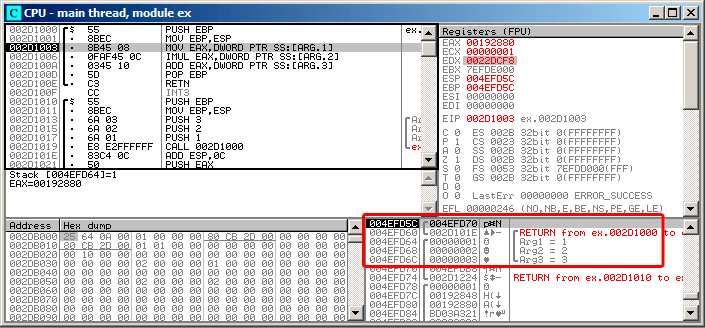
\includegraphics[scale=\FigScale]{patterns/05_passing_arguments/olly.png}
\caption{\olly: \RU{внутри ф-ции}\EN{inside of} \ttf{}\EN{ function}}
\label{fig:passing_arguments_olly}
\end{figure}
\fi

\subsection{GCC}

\RU{Скомпилируем то же в GCC 4.4.1 и посмотрим результат в \IDA:}
\EN{Let's compile the same in GCC 4.4.1 and let's see results in \IDA:}

\lstinputlisting[caption=GCC 4.4.1]{patterns/05_passing_arguments/gcc.asm}

\RU{Практически то же самое, если не считать мелких отличий описанных раннее.}
\EN{Almost the same result.}

\RU{После вызова обоих ф-ций, \glslink{stack pointer}{указатель стека} не возвращается назад, потому что предпоследняя
инструкция}\EN{The \gls{stack pointer} is not returning back after both function exeuction, because penultimate}
\TT{LEAVE} (\ref{x86_ins:LEAVE}) \RU{сделает это за один раз, в конце исполнения}\EN{instruction will do this,
at the end}.


\section{x64}

\index{x86-64}
\RU{В x86-64 всё немного иначе, здесь аргументы функции (4 или 6) передаются через регистры, 
а \gls{callee} из читает их из регистров, а не из стека.}
\EN{The story is a bit different in x86-64. Function arguments (first 4 or first 6 of them) 
are passed in registers i.e. the \gls{callee} reads them from registers instead of reading them from the stack.}

\subsection{MSVC}

\Optimizing MSVC:

\lstinputlisting[caption=\Optimizing MSVC 2012 x64]{patterns/05_passing_arguments/x64_MSVC_Ox.asm.\LANG}

\RU{Как видно, очень компактная функция \ttf берет аргументы прямо из регистров.}
\EN{As we can see, the compact function \ttf takes all its arguments from the registers.}
\RU{Инструкция \LEA используется здесь для сложения чисел. 
Должно быть компилятор посчитал, что это будет эффективнее использования \TT{ADD}.}
\EN{The \LEA instruction here is used for addition,
apparently the compiler considered it faster than \TT{ADD}.}
\index{x86!\Instructions!LEA}
\RU{В самой \main{} \LEA{} также используется для подготовки первого и третьего аргумента: должно быть,
компилятор решил, что \LEA{} будет работать здесь быстрее, чем загрузка значения в регистр при помощи \MOV.}
\EN{\LEA is also used in the \main function to prepare the first and third \ttf arguments. The compiler
must have decided that this would work faster than the usual way of loading values into a register using \MOV instruction.}

\RU{Попробуем посмотреть вывод неоптимизирующего MSVC}\EN{Let's take a look at the non-optimizing MSVC output}:

\lstinputlisting[caption=MSVC 2012 x64]{patterns/05_passing_arguments/x64_MSVC_IDA.asm.\LANG}

\RU{Немного путаннее: все 3 аргумента из регистров зачем-то сохраняются в стеке.}
\EN{It looks somewhat puzzling because all 3 arguments from the registers are saved to the stack for some reason.}
\index{Shadow space}
\label{shadow_space}
\RU{Это называется}\EN{This is called} ``shadow space''
\footnote{\href{http://go.yurichev.com/17256}{MSDN}}: 
\RU{каждая функция в Win64 может (хотя и не обязана) сохранять значения 4-х регистров там.}
\EN{every Win64 may (but is not required to) save all 4 register values there.}
\RU{Это делается по крайней мере из-за двух причин}\EN{This is done for two reasons}: 
1) \RU{в большой функции отвести целый регистр (а тем более 4 регистра) для входного аргумента 
слишком расточительно, так что к нему будет обращение через стек;}
\EN{it is too lavish to allocate a whole register (or even 4 registers) for an input argument,
so it will be accessed via stack;}
2) \RU{отладчик всегда знает, где найти аргументы функции в момент останова}\EN{the debugger is always
aware where to find the function arguments at a break}%
\footnote{\href{http://go.yurichev.com/17257}{MSDN}}.

\RU{Так что, какие-то большие функции могут сохранять входные аргументы в ``shadows space'' 
для использования в будущем, а небольшие функции, как наша, могут этого и не делать.}
\EN{So, some large functions can save their input arguments in the ``shadows space'' if they need to use them
during execution, but some small functions (like ours) may not do this.}

\RU{Место в стеке для ``shadow space'' выделяет именно \gls{caller}.}
\EN{It is a \gls{caller} responsibility to allocate ``shadow space'' in the stack.}

\ifdefined\IncludeGCC
\subsection{GCC}

\Optimizing GCC \RU{также делает понятный код}\EN{generates more or less understandable code}:

\lstinputlisting[caption=\Optimizing GCC 4.4.6 x64]{patterns/05_passing_arguments/x64_GCC_O3.s.\LANG}

\NonOptimizing GCC:

\lstinputlisting[caption=GCC 4.4.6 x64]{patterns/05_passing_arguments/x64_GCC.s.\LANG}

\index{Shadow space}
\RU{В соглашении о вызовах System V *NIX\cite{SysVABI} нет ``shadow space'', но \gls{callee} тоже иногда
должен сохранять где-то аргументы, потому что, опять же, регистров может и не хватить на все действия.
Что мы здесь и видим.}
\EN{There are no ``shadow space'' requirements in System V *NIX\cite{SysVABI}, but the \gls{callee} may need to save
its arguments somewhere in case of registers shortage.}

\subsection{GCC: uint64\_t \RU{вместо}\EN{instead of} int}

\RU{Наш пример работал с 32-битным \Tint, поэтому использовались 32-битные части регистров с префиксом \TT{E-}.}
\EN{Our example works with 32-bit \Tint, that is why 32-bit register parts are used (prefixed by \TT{E-}).}

\RU{Его можно немного переделать, чтобы он заработал с 64-битными значениями}\EN{It can be altered slightly
in order to use 64-bit values}:

\lstinputlisting{patterns/05_passing_arguments/ex64.c}

\lstinputlisting[caption=\Optimizing GCC 4.4.6 x64]{patterns/05_passing_arguments/ex64_GCC_O3_IDA.asm.\LANG}

\RU{Собствено, всё то же самое, только используются регистры \IT{целиком}, с префиксом \TT{R-}.}
\EN{The code is the same, but this time the \IT{full size} registers (prefixed by \TT{R-}) are used.}
\fi

\subsection{ARM}

\subsubsection{\NonOptimizingKeil + \ARMMode}

\begin{lstlisting}
.text:000000A4 00 30 A0 E1                 MOV     R3, R0
.text:000000A8 93 21 20 E0                 MLA     R0, R3, R1, R2
.text:000000AC 1E FF 2F E1                 BX      LR
...
.text:000000B0             main
.text:000000B0 10 40 2D E9                 STMFD   SP!, {R4,LR}
.text:000000B4 03 20 A0 E3                 MOV     R2, #3
.text:000000B8 02 10 A0 E3                 MOV     R1, #2
.text:000000BC 01 00 A0 E3                 MOV     R0, #1
.text:000000C0 F7 FF FF EB                 BL      f
.text:000000C4 00 40 A0 E1                 MOV     R4, R0
.text:000000C8 04 10 A0 E1                 MOV     R1, R4
.text:000000CC 5A 0F 8F E2                 ADR     R0, aD_0        ; "%d\n"
.text:000000D0 E3 18 00 EB                 BL      __2printf
.text:000000D4 00 00 A0 E3                 MOV     R0, #0
.text:000000D8 10 80 BD E8                 LDMFD   SP!, {R4,PC}
\end{lstlisting}

\IFRU{В функции \main просто вызываются две функции, в первую (\TT{f}) передается три значения.}
{In \main function, two other functions are simply called, and three values are passed to the 
first one (\TT{f}).}

\IFRU{Как я уже упоминал, первые 4 значения, в ARM обычно передаются в первых 4-х регистрах}
{As I mentioned before, in ARM, first 4 values are usually passed in first 4 registers} (\Rzero-\Rthree).

\IFRU{Функция }{}\TT{f}\IFRU{, как видно, использует три первых регистра (\Rzero-\Rtwo) как аргументы.}
{function, as it seems, use first 3 registers (\Rzero-\Rtwo) as arguments.}

\index{ARM!\Instructions!MLA}
\IFRU{Инструкция }{}\TT{MLA} (\IT{Multiply Accumulate}) \IFRU{перемножает два первых операнда (\Rthree и \Rone), 
прибавляет к произведению
третий операнд (\Rtwo) и помещает результат в нулевой операнд (\Rzero), через который, по стандарту, 
возвращаются значения функций.}
{instruction multiplicates two first operands (\Rthree and \Rone), adds third operand (\Rtwo) to product and places
result into zeroth operand (\Rzero), via which, by standard, values are returned from functions.}

\index{Fused multiply–add}
\IFRU{Умножение и сложение одновременно}{Multiplication and addition at once}\footnote{\WPMAO} 
(\IT{Fused multiply–add}) \IFRU{это много где применяемая операция, кстати, аналогичной
инструкции в x86 нет}{is very useful operation, by the way, there is no such instruction in x86}, 
\IFRU{если не считать новых FMA-инструкций}{if not to count new FMA-instruction}\footnote{\url{https://en.wikipedia.org/wiki/FMA_instruction_set}} \InENRU SIMD.

\IFRU{Самая первая инструкция}{The very first} \TT{MOV R3, R0}, \IFRU{по видимому, избыточна (можно было бы обойтись только одной инструкцией \TT{MLA})}
{instruction, apparently, redundant (single \TT{MLA} instruction could be used here instead)}, 
\IFRU{компилятор не оптимизировал её, ведь, это компиляция без оптимизации}{compiler was not optimized it,
since this is non-optimizing compilation}.

\index{ARM!\IFRU{Переключение режимов}{Mode switching}}
\index{ARM!\Instructions!BX}
\IFRU{Инструкция \TT{BX} возвращает управление по адресу записанному в \LR и, если нужно, 
переключает режимы процессора с thumb на ARM или наоборот.}
{\TT{BX} instruction returns control to the address stored in the \LR register and, if it is necessary, 
switches processor mode from thumb to ARM or vice versa.}
\IFRU{Это может быть необходимым потому, что, как мы видим, 
функции \TT{f} неизвестно, из какого кода она будет вызываться, из ARM или thumb.}
{This can be necessary since, as we can see, \TT{f} function is not aware, from which code it may be
called, from ARM or thumb.}
\IFRU{Поэтому, если она будет вызываться из кода thumb, \TT{BX} не только вернет
управление в вызывающую функцию, но также переключит процессор в режим thumb.}
{This, if it will be called from thumb code, \TT{BX} will not only return control to the calling function,
but also will switch processor mode to thumb mode.}
\IFRU{Либо не переключит, если функция вызывалась из кода для режима ARM.}
{Or not switch, if the function was called from ARM code.}

\subsubsection{\OptimizingKeil + \ARMMode}

\begin{lstlisting}
.text:00000098             f
.text:00000098 91 20 20 E0                 MLA     R0, R1, R0, R2
.text:0000009C 1E FF 2F E1                 BX      LR
\end{lstlisting}

\IFRU{А вот и функция \TT{f} скомпилированная компилятором Keil в режиме полной оптимизации}
{And here is \TT{f} function compiled by Keil compiler in full optimization mode} (\Othree).
\IFRU{Инструкция \MOV была соптимизирована и теперь \TT{MLA} использует все входящие регистры 
и помещает результат в \Rzero, как раз, где вызываемая функция будет его читать и использовать.}
{\MOV instruction was optimized (or reduced) and now \TT{MLA} uses all 
input registers and also places result right into \Rzero,
exactly where calling function will read it and use.}

\subsubsection{\OptimizingKeil + \ThumbMode}

\begin{lstlisting}
.text:0000005E 48 43                       MULS    R0, R1
.text:00000060 80 18                       ADDS    R0, R0, R2
.text:00000062 70 47                       BX      LR
\end{lstlisting}

\IFRU{В режиме thumb, инструкция \TT{MLA} недоступна, так что компилятору пришлось сгенерировать код, 
делающий обе операции по отдельности.}
{\TT{MLA} instruction is not available in thumb mode, so, compiler generates the code doing these two 
operations separately.}
\index{ARM!\Instructions!MULS}
\index{ARM!\Instructions!ADDS}
\IFRU{Первая инструкция \TT{MULS} умножает \Rzero на \Rone оставляя результат в \Rone.}
{First \TT{MULS} instruction multiply \Rzero by \Rone leaving result in the \Rone register.}
\IFRU{Вторая (\TT{ADDS}) складывает результат и \Rtwo, оставляя результат в \Rzero.}
{Second (\TT{ADDS}) instruction adds result and \Rtwo leaving result in the \Rzero register.}



\chapter{\RU{Еще о возвращаемых результатах}\EN{More about results returning}}

\index{x86!\Registers!EAX}
\RU{Результат выполнения функции в x86 обычно возвращается}
\EN{In x86, the result of function execution is usually returned}
\footnote{\Seealso: 
MSDN: Return Values (C++): \href{http://go.yurichev.com/17258}{MSDN}}
\RU{через регистр \EAX, 
а если результат имеет тип байт или символ (\Tchar), 
то в самой младшей части \EAX ~--- \AL. Если функция возвращает число с плавающей запятой, 
то будет использован регистр FPU \ST{0}.
\ifdefined\IncludeARM
\index{ARM!\Registers!R0}
В ARM обычно результат возвращается в регистре \Reg{0}.
\fi
}
\EN{in the \EAX register. 
If it is byte type or a character (\Tchar), then the lowest part of register \EAX (\AL) is used. 
If a function returns a \Tfloat number, the FPU register \ST{0} is used instead.
\ifdefined\IncludeARM
\index{ARM!\Registers!R0}
In ARM, the result is usually returned in the \Reg{0} register.
\fi
}

\section{\RU{Попытка использовать результат ф-ции возвращающей \Tvoid}
\EN{Attempt to use the result of a function returning \Tvoid}}

\RU{Кстати, что будет если возвращаемое значение в ф-ции \main объявлять не как \Tint а как \Tvoid?}
\EN{So, what if the \main function return value was declared of type \Tvoid and not \Tint?}

\RU{Т.н. startup-код вызывает \main примерно так:}
\EN{The so-called startup-code is calling \main roughly as follows:}

\begin{lstlisting}
push envp
push argv
push argc
call main
push eax
call exit
\end{lstlisting}

\RU{Т.е., иными словами:}\EN{In other words:}

\begin{lstlisting}
exit(main(argc,argv,envp));
\end{lstlisting}

\RU{Если вы объявите \main как \Tvoid, и ничего не будете возвращать явно (при помощи выражения \IT{return}), 
то в единственный аргумент exit() попадет
то, что лежало в регистре \EAX на момент выхода из \main.}
\EN{If you declare \main as \Tvoid, nothing will be returned explicitly (using the \IT{return} statement),
then something random, that was stored in the \EAX register at the end of \main will become 
the sole argument of the exit() function.}
\RU{Там, скорее всего, будет какие-то случайное число, оставшееся от работы вашей ф-ции.}
\EN{Most likely, there will be a random value, left from your function execution, }
\RU{Так что, код завершения программы будет псевдослучайным.}
\EN{so the exit code of program will be pseudorandom.} \\

\RU{Я могу это проиллюстрировать}\EN{I can illustrate this fact}. 
\RU{Заметьте что у ф-ции}\EN{Please note that here the} \main \RU{тип возвращаемого значения именно}\EN{function 
has a} \Tvoid\EN{ return type}:

\begin{lstlisting}
#include <stdio.h>

void main()
{
	printf ("Hello, world!\n");
};
\end{lstlisting}

\RU{Скомпилируем в}\EN{Let's compile it in} Linux.

\index{puts() \RU{вместо}\EN{instead of} printf()}
GCC 4.8.1 \RU{заменила}\EN{replaced} \printf \RU{на}\EN{with} \puts 
\ifx\LITE\undefined
(\RU{мы видели это прежде}\EN{we have seen this before}: \myref{puts})
\fi
, \RU{но это нормально, потому что}\EN{but that's OK, since} \puts \RU{возвращает количество
выведенных символов, так же как и}\EN{returns the number of characters printed out, just like} \printf.
\RU{Обратите внимание на то что}\EN{Please notice that} \EAX \RU{не обнуляется перед выходом их}\EN{is not 
zeroed before} \main\EN{'s end}.
\RU{Это значит,}\EN{This means that the value of} \EAX \RU{перед выходом из}\EN{at the end of} \main 
\RU{будет содержать то, что}\EN{will contain what} \puts \RU{оставит там}\EN{has left there}.

\begin{lstlisting}[caption=GCC 4.8.1]
.LC0:
	.string	"Hello, world!"
main:
	push	ebp
	mov	ebp, esp
	and	esp, -16
	sub	esp, 16
	mov	DWORD PTR [esp], OFFSET FLAT:.LC0
	call	puts
	leave
	ret
\end{lstlisting}

\index{bash}
\RU{Напишем небольшой скрипт на bash, показывающий статус возврата (``exit status'' или ``exit code'')}
\EN{Let' s write a bash script that shows the exit status}:

\begin{lstlisting}[caption=tst.sh]
#!/bin/sh
./hello_world
echo $?
\end{lstlisting}

\RU{И запустим}\EN{And run it}:

\begin{lstlisting}
$ tst.sh 
Hello, world!
14
\end{lstlisting}

$14$ \RU{это как раз количество выведенных символов}\EN{is the number of characters printed}.

\section{\RU{Что если не использовать результат ф-ции?}\EN{What if we do not use the function result?}}

\RU{\printf возвращает количество успешно выведенных символов, но результат работы этой ф-ции 
редко используется на практике.}
\EN{\printf returns the count of characters successfully output, but the result of this function 
is rarely used in practice.}
\RU{Можно даже явно вызывать ф-ции, чей смысл именно в возвращаемых значениях, но явно не использовать их:}
\EN{It is also possible to call a function whose essence is in returning a value, and not use it:}

\begin{lstlisting}
int f()
{
    // skip first 3 random values
    rand();
    rand();
    rand();
    // and use 4th
    return rand();
};
\end{lstlisting}

\EN{The result of the rand() function will always be left in \EAX, in all four cases.}
\RU{Результат работы rand() будет оставаться в \EAX во всех четырех случаях.}
\EN{But in the first 3 cases, the value in \EAX will be just thrown away.}
\RU{Но в первых трех случаях, значение лежащее в \EAX, будет просто выброшено.}

\ifx\LITE\undefined
\section{\RU{Возврат структуры}\EN{Returning a structure}}

\index{\CLanguageElements!return}
\RU{Вернемся к тому факту, что возвращаемое значение остается в регистре \EAX}
\EN{Let's go back to the fact that the return value is left in the \EAX register}.
\RU{Вот почему старые компиляторы Си не способны создавать функции, возвращающие нечто большее, нежели 
помещается 
в один регистр (обычно, тип \Tint), а когда нужно, приходится возвращать через указатели, указываемые 
в аргументах.}
\EN{That is why old C compilers cannot create functions capable of returning something that does not fit in one 
register (usually \Tint), but if one needs it, one have to return information via pointers passed 
as function's arguments.}
\RU{Так что, как правило, если ф-ция должна вернуть несколько значений, она возвращает только одно, 
а остальные --- через указатели.}
\EN{So, usually, if a function needs to return several values, it returns only one, and 
all the rest---via pointers.}
\RU{Хотя, позже и стало возможным, вернуть, скажем, целую структуру, но этот метод до сих пор не 
очень популярен. 
Если функция должна вернуть структуру, вызывающая функция должна сама, скрыто и прозрачно для программиста, 
выделить место и передать указатель на него в качестве первого аргумента. Это почти то же самое 
что и сделать это вручную, но компилятор прячет это.}
\EN{Now it has become possible to return, let's say, an entire structure, but that is still not very popular. 
If a function has to return a large structure, the \gls{caller} must allocate it and pass a pointer to it via the first argument, transparently for the programmer. 
That is almost the same as to pass a pointer in the first argument manually, but the compiler hides it.}

\RU{Небольшой пример:}\EN{Small example:}

\lstinputlisting{patterns/06_return_results/6_1.c}

\dots \RU{получим}\EN{what we got} (MSVC 2010 \Ox):

\lstinputlisting{patterns/06_return_results/6_1.asm}

\RU{Имя внутреннего макроса для передачи указателя на структуру здесь это \TT{\$T3853}.}
\EN{The macro name for internal passing of pointer to a structure her is \TT{\$T3853}.}

\index{\CLanguageElements!C99}
\RU{Этот пример можно даже переписать, используя расширения C99}\EN{This example can be rewritten using
the C99 language extensions}:

\lstinputlisting{patterns/06_return_results/6_1_C99.c}

\lstinputlisting[caption=GCC 4.8.1]{patterns/06_return_results/6_1_C99.asm}

\RU{Как видно, ф-ция просто заполняет поля в структуре, выделенной вызывающей ф-цией. 
Как если бы передавался просто указатель на структуру.
Так что никаких проблем с эффективностью нет.}
\EN{As we see, the function is just filling the structure's fields allocated by
the caller function,
as if a pointer to the structure was passed.
So there are no performance drawbacks.}
\fi

\section{\IFRU{Указатели}{Pointers}}
\index{\CLanguageElements!\Pointers}
\label{label_pointers}

\newcommand{\ttf}{\TT{f1()}}

\IFRU{Указатели также часто используются для возврата значений из функции (вспомните случай
со \scanf{}~(\ref{label_scanf}))}
{Pointers are often used to return values from function (recall \scanf case~(\ref{label_scanf}))}.
\IFRU{Например, когда функции нужно вернуть сразу два значения}
{For example, when function should return two values}.

\subsection{\IFRU{Пример с глобальными переменными}{Global variables example}}

\lstinputlisting{patterns/061_pointers/global.c}

\IFRU{Это компилируется в}{This compiling into}:

\lstinputlisting[caption=\Optimizing MSVC 2010 (/Ox /Ob0)]{patterns/061_pointers/global.asm}

\index{\olly}
\IFRU{Посмотрим это в}{Let's see this in} \olly: \figname \ref{fig:pointers_olly_global_1}.
\IFRU{В начале адреса обоих глобальных переменных передаются в}{At first, global
variables addresses are passed into} \ttf.
\IFRU{Можно нажать}{We can click} ``Follow in dump'' \IFRU{на элементе стека и в окне слева 
увидим место в сегменте данных выделенных для двух переменных}{on the stack element, and we will see 
a place in data segment allocated for two variables}.
\IFRU{Эти переменные обнулены, потому что, по стандарту, неинициализированные данные (\ac{BSS}) 
обнуляются перед началом исполнения}
{These variables are cleared, because non-initialized data (\ac{BSS}) are cleared before
execution begin}.
\IFRU{И они находятся в сегменте данных, о чем можно удостовериться нажав}
{They are residing in data segment, we can be sure it is so, by pressing} Alt-M \IFRU{и увидев карту
памяти}{and seeing memory map}: \figname \ref{fig:pointers_olly_global_5}.

\IFRU{Трассируем}{Let's trace} (F7) \IFRU{до начала исполнения}{until execution of} \ttf 
\figname \ref{fig:pointers_olly_global_2}.
\IFRU{В стеке видны и значения}{Two values are seen in the stack} $456$ (\TT{0x1C8}) \AndENRU 
$123$ (\TT{0x7B}), \IFRU{а также адреса двух глобальных переменных}{and two global variables addresses
as well}.

\IFRU{Трассируем до конца}{Let's trace until the end of} \ttf.
\IFRU{Мы видим в окне слева, как результаты вычисления появились в глобальных переменных}
{At the window at left we see how calculation results are appeared in the gloval variables} 
\figname \ref{fig:pointers_olly_global_3}.

\IFRU{Теперь из глобальных переменных значения загружаются в регистры для передачи в}
{Now values of global variables are loaded into registers for passing into} \printf:
\figname \ref{fig:pointers_olly_global_4}.

\begin{figure}[H]
\centering
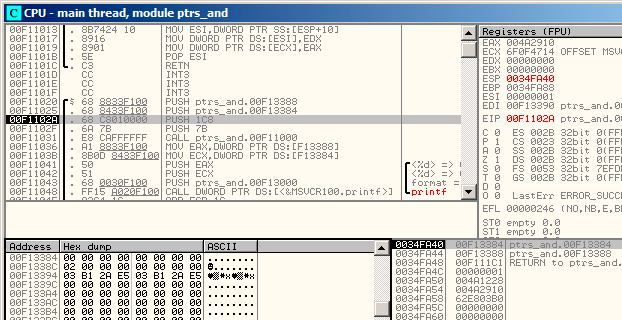
\includegraphics[scale=0.66]{patterns/061_pointers/olly_global1.png}
\caption{\olly: \IFRU{передаются адреса двух глобальных переменных в}
{global variables addresses are passing into} \ttf}
\label{fig:pointers_olly_global_1}
\end{figure}

\begin{figure}[H]
\centering
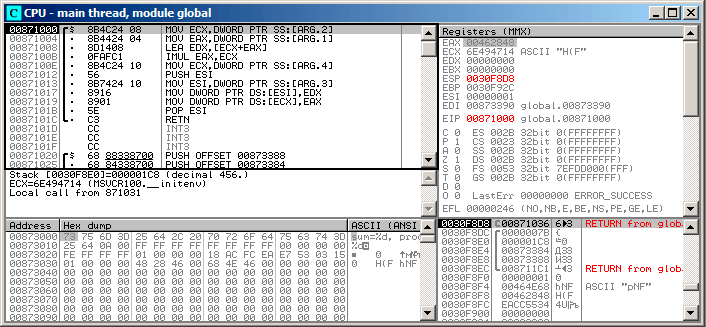
\includegraphics[scale=0.66]{patterns/061_pointers/olly_global2.png}
\caption{\olly: \IFRU{начало работы \ttf}{\ttf is started}}
\label{fig:pointers_olly_global_2}
\end{figure}

\begin{figure}[H]
\centering
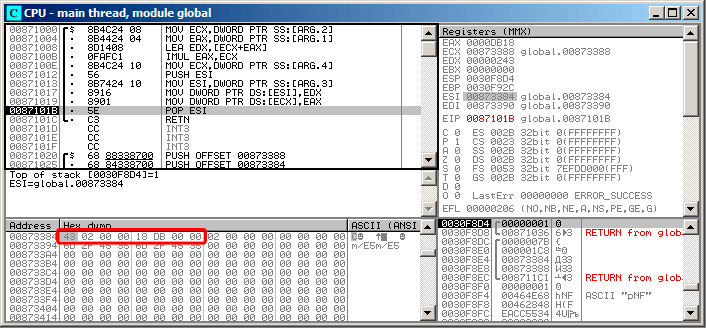
\includegraphics[scale=0.66]{patterns/061_pointers/olly_global3.png}
\caption{\olly: \ttf \IFRU{заканчивает работу}{finishes}}
\label{fig:pointers_olly_global_3}
\end{figure}

\begin{figure}[H]
\centering
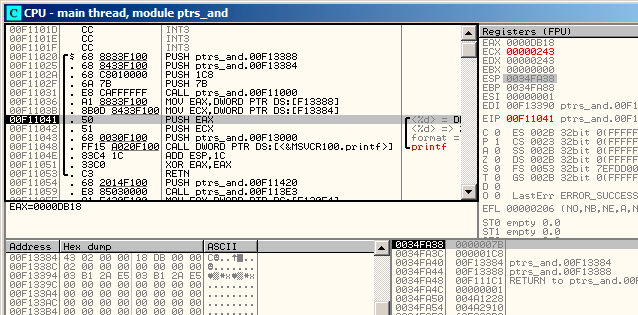
\includegraphics[scale=0.66]{patterns/061_pointers/olly_global4.png}
\caption{\olly: \IFRU{адреса глобальных переменных передаются в}
{global variables addresses are passed into} \printf}
\label{fig:pointers_olly_global_4}
\end{figure}

\begin{figure}[H]
\centering
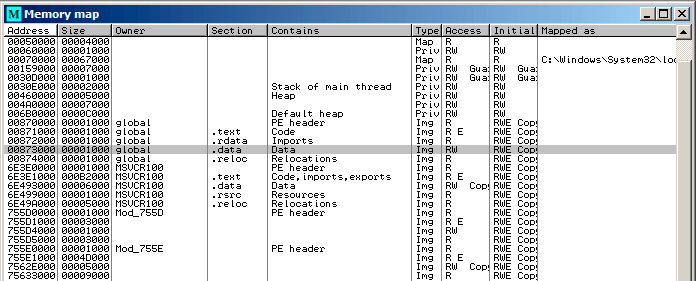
\includegraphics[scale=0.66]{patterns/061_pointers/olly_global5.png}
\caption{\olly: \IFRU{карта памяти}{memory map}}
\label{fig:pointers_olly_global_5}
\end{figure}

\subsection{\IFRU{Пример с локальными переменными}{Local variables example}}

\IFRU{Немного переделаем пример}{Let's rework our example slightly}:

\lstinputlisting[caption=\IFRU{теперь переменные локальные}
{now variables are local}]{patterns/061_pointers/local_\IFRU{ru}{en}.c}

\RU{Код ф-ции }\ttf \IFRU{не изменится}{function code will not changed}.
\IFRU{Изменится только \main}{Only \main code will}:

\lstinputlisting[caption=\Optimizing MSVC 2010 (/Ox /Ob0)]{patterns/061_pointers/local.asm}

\newcommand{\PtrsAddresses}{\TT{0x35FCF4} \AndENRU \TT{0x35FCF8}\xspace}

\IFRU{Снова посмотрим в}{Let's again take a look into} \olly.
\IFRU{Адреса локальных переменных в стеке это}{Local variable addresses in the stack are} \PtrsAddresses.
\IFRU{Видно как они заталкиваются в стек}{We see how these are pushed into the stack}: 
\figname \ref{fig:pointers_olly_stk_1}.

\IFRU{Начало работы \ttf}{\ttf is started}.
\IFRU{В стеке по адресам}{Random garbage are at} \PtrsAddresses \IFRU{пока находится случайный мусор}
{so far} \figname \ref{fig:pointers_olly_stk_2}.

\IFRU{Конец работы \ttf}{\ttf finished}.
\IFRU{В стеке по адресам \PtrsAddresses теперь значения \TT{0xDB18} \AndENRU \TT{0x243}, 
это результаты работы \ttf}
{There are \TT{0xDB18} \AndENRU \TT{0x243} now at \PtrsAddresses addresses, these values are
\ttf function result}.

\begin{figure}[H]
\centering
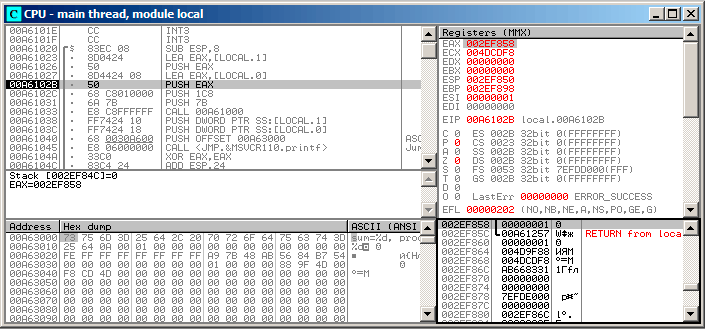
\includegraphics[scale=0.66]{patterns/061_pointers/olly_stk1.png}
\caption{\olly: \IFRU{адреса локальных переменных заталкиваются в стек}{addresses of local variables are
pushed into the stack}}
\label{fig:pointers_olly_stk_1}
\end{figure}

\begin{figure}[H]
\centering
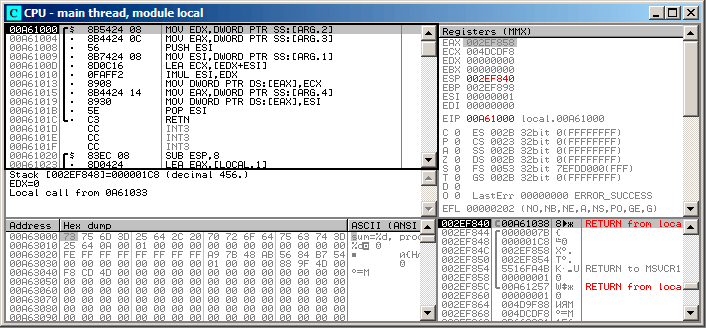
\includegraphics[scale=0.66]{patterns/061_pointers/olly_stk2.png}
\caption{\olly: \ttf \IFRU{начинает работу}{starting}}
\label{fig:pointers_olly_stk_2}
\end{figure}

\begin{figure}[H]
\centering
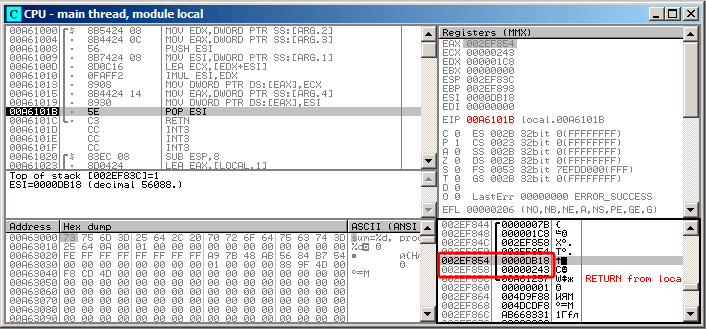
\includegraphics[scale=0.66]{patterns/061_pointers/olly_stk3.png}
\caption{\olly: \ttf \IFRU{заканчивает работу}{finished}}
\label{fig:pointers_olly_stk_3}
\end{figure}

\subsection{\IFRU{Вывод}{Conclusion}}

\IFRU{\ttf может одинаково хорошо возвращать результаты работы в любые места памяти, 
находящиеся где угодно}{\ttf can return results to any place in memory, located anywhere}.
\IFRU{В этом суть и удобство указателей}{This is essence and usefulness of pointers}.

\IFRU{Кстати,}{By the way, \Cpp} \IT{references} \IFRU{в \Cpp работают точно так же}{works just in the
same way}. \IFRU{Читайте больше об этом}{Read more about them}: (\ref{cpp_references}).


\chapter{\RU{Условные переходы}\EN{Conditional jumps}}
\label{sec:Jcc}
\index{\CLanguageElements!if}

% sections
\section{\RU{Простой пример}\EN{Simple example}}

\lstinputlisting{patterns/07_jcc/simple/ex.c}

% subsections
\subsection{x86}

\subsubsection{x86 + MSVC}

\RU{Имеем в итоге функцию \TT{f\_signed()}:}\EN{What we have in the \TT{f\_signed()} function:}

\lstinputlisting[caption=\NonOptimizing MSVC 2010]{patterns/07_jcc/simple/signed_MSVC.asm}

\index{x86!\Instructions!JLE}
\RU{Первая инструкция}\EN{First instruction} \JLE \RU{значит}\EN{means} \IT{Jump if Less or Equal}. 
\RU{То есть, если второй операнд больше первого или 
равен ему, произойдет переход туда, где будет следующая проверка.}
\EN{In other words, if second operand is 
larger than first or equal, control flow will be passed to address or label mentioned in instruction.}
\RU{А если это условие не срабатывает, то есть второй операнд меньше первого, то перехода не будет, 
и сработает первый \printf.}
\EN{But if this condition will not trigger (second operand less than first), control flow will 
not be altered and first \printf will be called.}
\index{x86!\Instructions!JNE}
\RU{Вторая проверка это}\EN{The second check is} \JNE: \IT{Jump if Not Equal}.
\RU{Переход не произойдет, если операнды равны}\EN{Control flow will not altered if operands are 
equals to each other}.
\index{x86!\Instructions!JGE}
\RU{Третья проверка}\EN{The third check is} \JGE: \IT{Jump if Greater or Equal}\EMDASH{}\RU{переход 
если первый операнд больше второго или равен ему}\EN{jump if the first operand is larger than 
the second or if they are equals to each other}.
\RU{Кстати, если все три условных перехода сработают, ни один \printf не вызовется. 
Но, без внешнего вмешательства, это невозможно.}
\EN{By the way, if all three conditional jumps are triggered, no \printf will be called whatsoever. 
But, without special intervention, it is impossible.}

\RU{Функция }\TT{f\_unsigned()} \RU{точно такая же, за тем исключением, что используются инструкции 
\JBE и \JAE вместо \JLE и \JGE, об этом читайте ниже}
\EN{function is likewise, with the exception the \JBE and \JAE instructions
are used here instead of 
\JLE and \JGE, see below about it}:

\RU{Далее функция \TT{f\_unsigned()}}
\EN{Now let's take a look to the \TT{f\_unsigned()} function}

\lstinputlisting[caption=GCC]{patterns/07_jcc/simple/unsigned_MSVC.asm}

\index{x86!\Instructions!JBE}
\index{x86!\Instructions!JAE}
\RU{Здесь все то же самое, только инструкции условных переходов немного другие}
\EN{Almost the same, with exception of instructions}:
\JBE\EMDASH{}\IT{Jump if Below or Equal} \AndENRU \JAE\EMDASH{}\IT{Jump if Above or Equal}.
\RU{Эти инструкции}\EN{These instructions} (\JA/\JAE/\JB/\JBE) 
\RU{отличаются от}\EN{are distinct from} \JG/\JGE/\JL/\JLE \RU{тем}\EN{in that way}, 
\RU{что работают с беззнаковыми переменными}\EN{they works with unsigned numbers}.

\index{x86!\Instructions!JA}
\index{x86!\Instructions!JB}
\index{x86!\Instructions!JG}
\index{x86!\Instructions!JL}
\index{Signed numbers}
\RU{Отступление: смотрите также секцию о представлении знака в числах}
\EN{See also section about signed number representations}~(\ref{sec:signednumbers}).
\RU{Таким образом, увидев где используется \JG/\JL вместо \JA/\JB и наоборот, 
можно сказать почти уверенно насчет того, 
является ли тип переменной знаковым (signed) или беззнаковым (unsigned).}
\EN{So, where we see usage of \JG/\JL instead of \JA/\JB or otherwise, 
we can almost be sure about signed or unsigned type of variable.}

\RU{Далее функция \main, где ничего нового для нас нет}
\EN{Here is also \main function, where nothing much new to us}:

\lstinputlisting[caption=\main]{patterns/07_jcc/simple/main_MSVC.asm}

\ifdefined\IncludeOlly
\input{patterns/07_jcc/simple/olly.tex}
\fi

\clearpage
\subsubsection{x86 + MSVC + Hiew}
\index{Hiew}

\RU{Можем попробовать модифицировать исполняемый файл так}\EN{We can try patch executable file in that way}, 
\RU{чтобы ф-ция}\EN{that} \TT{f\_unsigned()} \RU{всегда показывала}\EN{function will always print} ``a==b'', 
\RU{при любых входящих значениях}\EN{for any input values}.

\RU{Вот как она выглядит в}\EN{Here is how it looks in} Hiew:

\begin{figure}[H]
\centering
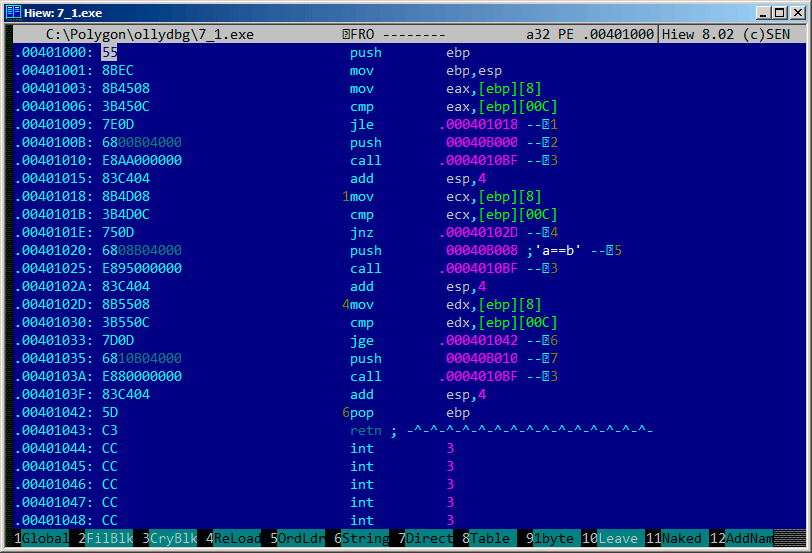
\includegraphics[scale=\FigScale]{patterns/07_jcc/simple/hiew_unsigned1.png}
\caption{Hiew: \RU{функция }\TT{f\_unsigned()}\EN{ function}}
\label{fig:jcc_hiew_1}
\end{figure}

\RU{Собственно, задаче три}\EN{Essentially, we've got three tasks}:
\begin{itemize}
\item \RU{заставить первый переход срабатывать всегда}\EN{force first jump to be always triggered};
\item \RU{заставить второй переход не срабатывать никогда}\EN{force second jump to be never triggered};
\item \RU{заставить третий переход срабатывать всегда}\EN{force third jump to be always triggered}.
\end{itemize}

\RU{Так мы направим путь исполнения кода (code flow) во второй}\EN{Thus we can point code flow
into the second} \printf,
\RU{и он всегда будет срабатывать и выводить на консоль}\EN{and it always print} ``a==b''.

\RU{Для этого нужно пропатчить три инструкции (или байта)}\EN{Three instructions (or bytes) should be patched}:

\begin{itemize}
\item \RU{Первый переход теперь будет}\EN{The first jump will now be} \JMP, \RU{но смещение перехода 
(\gls{jump offset}) останется прежним}\EN{but \gls{jump offset} will be same}.

\item \RU{Второй переход может быть и будет срабатывать иногда, но в любом случае он будет совершать переход
только на следующую инструкцию, потому что мы выставляем смещение перехода (\gls{jump offset}) в 0}
\EN{The second jump may be triggered sometimes, but in any case it will jump to the next
instruction, because, we set \gls{jump offset} to 0}.
\RU{В этих инструкциях, смещение перехода просто прибавляется к адресу следующей инструкции}
\EN{\Gls{jump offset} is just to be added to the address of the next instruction in these instructions}.
\RU{И когда смещение 0, то тогда и переход будет на следующую инструкцию}\EN{So if offset is 0,
jump will be done to the next instruction}.

\item \RU{Третий переход конвертируем в \JMP точно так же, как и первый, он будет срабатывать всегда}
\EN{The third jump we convert into \JMP just as the first one, so it will be triggered always}.
\end{itemize}

\clearpage
\RU{Что и делаем}\EN{That's what we do}:

\begin{figure}[H]
\centering
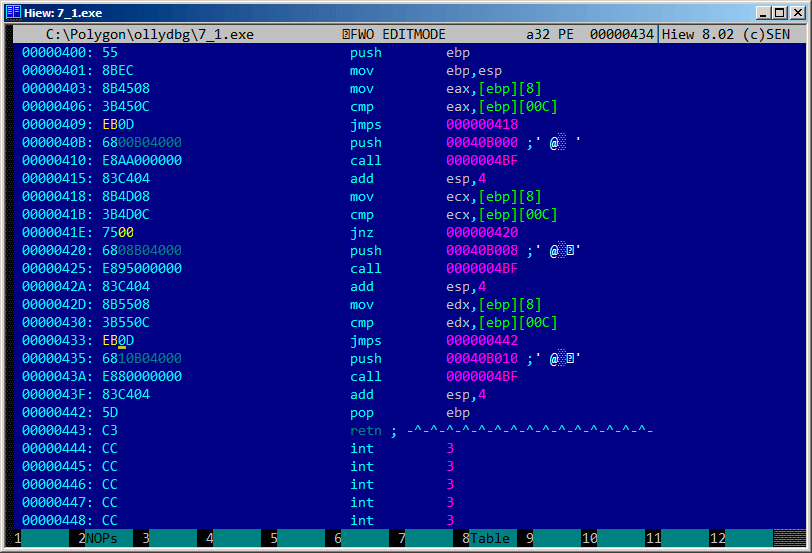
\includegraphics[scale=\FigScale]{patterns/07_jcc/simple/hiew_unsigned2.png}
\caption{Hiew: \RU{модифицируем функцию}\EN{let's modify} \TT{f\_unsigned()}\EN{ function}}
\label{fig:jcc_hiew_2}
\end{figure}

\RU{Если забыть про какой-то из переходов, то тогда будет срабатывать несколько вызовов \printf, 
а нам ведь нужно чтобы исполнялся только один.}
\EN{If we could forget about any of these jumps, then several
\printf calls may execute, but this is not behaviour we're need.}

\subsubsection{\NonOptimizing GCC}

\index{puts() \RU{вместо}\EN{instead of} printf()}
\NonOptimizing GCC 4.4.1 \RU{производит почти такой же код, за исключением}
\EN{produce almost the same code, but with} \puts~(\ref{puts}) \RU{вместо}\EN{instead of} \printf.

\subsubsection{\Optimizing GCC}

\RU{Наблюдательный читатель может спросить, зачем исполнять \CMP так много раз,
если флаги всегда одни и те же}\EN{Observant reader may ask, why to execute \CMP several times, 
if flags are same after each execution}?
\RU{По видимому, оптимизирующий MSVC не может этого делать, но GCC 4.8.1 делает больше оптимизаций:}
\EN{Perhaps, optimizing MSVC can't do this, but optimizing GCC 4.8.1 can optimize more deeply:}

\lstinputlisting[caption=GCC 4.8.1 f\_signed()]{patterns/07_jcc/simple/GCC_O3_signed.asm}

% should be here instead of 'switch' section?
\RU{Мы здесь также видим}\EN{We also see} \TT{JMP puts} \RU{вместо}\EN{here instead of} \TT{CALL puts / RETN}.
\RU{Этот прием будет описан немного позже}\EN{This kind of trick will be described later}: \ref{JMP_instead_of_RET}.

\RU{Нужно сказать что x86-код такого типа редок}\EN{Needless to say, that this type of x86 code 
is somewhat rare}.
MSVC 2012, \RU{как видно, не может генерировать подобное}\EN{as it seems, can't generate such code}.
\RU{С другой стороны, программисты на ассемблере прекрасно осведомлены о том, что инструкции}\EN{On the other hand, 
assembly language programmers are fully aware of the fact that} \TT{Jcc} \RU{можно располагать последовательно}
\EN{instructions can be stacked}.
\RU{Так что если вы видите это где-то, имеется немалая вероятность, что этот фрагмент кода был написан вручную}
\EN{So if you see it somewhere, it may be a good probability that the code is hand-written}.

\RU{Ф-ция }\TT{f\_unsigned()} \RU{получилась не настолько эстетически короткой}\EN{function is not that 
\ae{}sthetically short}:

\lstinputlisting[caption=GCC 4.8.1 f\_unsigned()]{patterns/07_jcc/simple/GCC_O3_unsigned.asm.\LANG}

\RU{Но тем не менее, здесь 2 инструкции \TT{CMP} вместо трех.}
\EN{But nevertheless, there are two \TT{CMP} instructions instead of three.}
\RU{Так что, алгоритмы оптимизации}\EN{So, optimization algorithms of} GCC 4.8.1 
\RU{наверное, еще пока не идеальны}\EN{are probably not always perfect yet}.


\subsectionold{ARM}

% subsubsections here
\EN{\input{patterns/07_jcc/simple/ARM/ARM32_EN}}
\RU{\input{patterns/07_jcc/simple/ARM/ARM32_RU}}
\EN{\input{patterns/07_jcc/simple/ARM/ARM64_EN}}
\RU{\input{patterns/07_jcc/simple/ARM/ARM64_RU}}


\EN{\subsection{MIPS}

One distinctive MIPS feature is the absence of flags.
Apparently, it was done to simplify the analysis of data dependencies.

\myindex{x86!\Instructions!SETcc}
\myindex{MIPS!\Instructions!SLT}
\myindex{MIPS!\Instructions!SLTU}

There are instructions similar to \INS{SETcc} in x86: \INS{SLT} (\q{Set on Less Than}: signed version) and 
\INS{SLTU} (unsigned version).
These instructions sets destination register value to 1 if the condition is true or to 0 if otherwise.

\myindex{MIPS!\Instructions!BEQ}
\myindex{MIPS!\Instructions!BNE}

The destination register is then checked using \INS{BEQ} (\q{Branch on Equal}) or \INS{BNE} (\q{Branch on Not Equal}) 
and a jump may occur.
So, this instruction pair has to be used in MIPS for comparison and branch.
Let's first start with the signed version of our function:

\lstinputlisting[caption=\NonOptimizing GCC 4.4.5 (IDA)]{patterns/07_jcc/simple/O0_MIPS_signed_IDA.lst.\LANG}

\INS{SLT REG0, REG0, REG1} is reduced by IDA to its 
shorter form \INS{SLT REG0, REG1}.
\myindex{MIPS!\Pseudoinstructions!BEQZ}

We also see there \INS{BEQZ} pseudoinstruction (\q{Branch if Equal to Zero}), 
which are in fact \INS{BEQ REG, \$ZERO, LABEL}.

\myindex{MIPS!\Instructions!SLTU}

The unsigned version is just the same, but \INS{SLTU} (unsigned version, hence \q{U} in name) is used instead of \INS{SLT}:

\lstinputlisting[caption=\NonOptimizing GCC 4.4.5 (IDA)]{patterns/07_jcc/simple/O0_MIPS_unsigned_IDA.lst}

}
\RU{\subsubsection{MIPS}

Одна отличительная особенность MIPS это отсутствие регистра флагов.
Очевидно, так было сделано для упрощения анализа зависимости данных (data dependency).

\myindex{x86!\Instructions!SETcc}
\myindex{MIPS!\Instructions!SLT}
\myindex{MIPS!\Instructions!SLTU}
Так что здесь есть инструкция, похожая на \INS{SETcc} в x86: \INS{SLT} (\q{Set on Less Than}~--- установить если
меньше чем, знаковая версия) и \INS{SLTU} (беззнаковая версия).
Эта инструкция устанавливает регистр-получатель в 1 если условие верно или в 0 в противном случае.

\myindex{MIPS!\Instructions!BEQ}
\myindex{MIPS!\Instructions!BNE}
Затем регистр-получатель проверяется, используя инструкцию 
\INS{BEQ} (\q{Branch on Equal} --- переход если равно) или \INS{BNE} (\q{Branch on Not Equal} --- переход если не равно) 
и может произойти переход.
Так что эта пара инструкций должна использоваться в MIPS для сравнения и перехода.
Начнем с знаковой версии нашей функции:

\lstinputlisting[caption=\NonOptimizing GCC 4.4.5 (IDA)]{patterns/07_jcc/simple/O0_MIPS_signed_IDA_RU.lst}

\INS{SLT REG0, REG0, REG1} сокращается в IDA до более короткой формы \INS{SLT REG0, REG1}.
\myindex{MIPS!\Pseudoinstructions!BEQZ}
Мы также видим здесь псевдоинструкцию \INS{BEQZ} (\q{Branch if Equal to Zero}~--- переход если равно нулю), 
которая, на самом деле, \INS{BEQ REG, \$ZERO, LABEL}.

\myindex{MIPS!\Instructions!SLTU}
Беззнаковая версия точно такая же, только здесь используется \INS{SLTU} (беззнаковая версия, 
отсюда \q{U} в названии) вместо \INS{SLT}:

\lstinputlisting[caption=\NonOptimizing GCC 4.4.5 (IDA)]{patterns/07_jcc/simple/O0_MIPS_unsigned_IDA.lst}

}

\section{\RU{Вычисление абсолютной величины}\EN{Calculating absolute value}}
\label{sec:abs}

\RU{Это простая функция}\EN{A simple function}:

\lstinputlisting{abs.c}

\subsection{\Optimizing MSVC}

\RU{Обычный способ генерации кода:}
\EN{This is how the code is usually generated:}

\lstinputlisting[caption=\Optimizing MSVC 2012 x64]{patterns/07_jcc/abs/abs_MSVC2012_Ox_x64.asm.\LANG}

\ifdefined\IncludeGCC
\RU{GCC 4.9 делает почти то же самое.}
\EN{GCC 4.9 does mostly the same.}
\fi

\ifdefined\IncludeARM
\subsection{\OptimizingKeilVI: \ThumbMode}

\lstinputlisting[caption=\OptimizingKeilVI: \ThumbMode]{patterns/07_jcc/abs/abs_Keil_thumb_O3.s.\LANG}

\myindex{ARM!\Instructions!RSB}
\RU{В ARM нет инструкции для изменения знака, так что компилятор Keil использует инструкцию \q{Reverse Subtract},
которая просто вычитает, но с операндами, переставленными наоборот.}
\EN{ARM lacks a negate instruction, so the Keil compiler uses the \q{Reverse Subtract} instruction, which just subtracts with reversed operands.}

\subsection{\OptimizingKeilVI: \ARMMode}

\RU{В режиме ARM можно добавлять коды условий к некоторым инструкций, что компилятор Keil и сделал:}
\EN{It is possible to add condition codes to some instructions in ARM mode, so that is what the Keil compiler does:}

\lstinputlisting[caption=\OptimizingKeilVI: \ARMMode]{patterns/07_jcc/abs/abs_Keil_ARM_O3.s.\LANG}

\RU{Теперь здесь нет условных переходов и это хорошо:}
\EN{Now there are no conditional jumps and this is good:} 
\myref{branch_predictors}.

\subsection{\NonOptimizing GCC 4.9 (ARM64)}

\myindex{ARM!\Instructions!XOR}
\RU{В ARM64 есть инструкция NEG для смены знака:}
\EN{ARM64 has instruction NEG for negating:}

\lstinputlisting[caption=\Optimizing GCC 4.9 (ARM64)]{patterns/07_jcc/abs/abs_GCC49_ARM64_O0.s.\LANG}
\fi

\ifdefined\IncludeMIPS
\subsection{MIPS}

\lstinputlisting[caption=\Optimizing GCC 4.4.5 (IDA)]{patterns/07_jcc/abs/MIPS_O3_IDA.lst.\LANG}

\myindex{MIPS!\Instructions!BLTZ}
\RU{Видим здесь новую инструкцию}\EN{Here we see a new instruction}: BLTZ (\q{Branch if Less Than Zero}).
\myindex{MIPS!\Instructions!SUBU}
\myindex{MIPS!\Pseudoinstructions!NEGU}
\RU{Тут есть также псевдоинструкция NEGU, которая на самом деле вычитает из нуля.}
\EN{There is also the NEGU pseudoinstruction, which just does subtraction from zero.}
\RU{Суффикс \q{U} в обоих инструкциях SUBU и NEGU означает, что при целочисленном переполнении исключение не
сработает.}
\EN{The \q{U} suffix in both SUBU and NEGU implies that no exception to be raised in case of integer overflow.}

\fi

\subsection{\RU{Версия без переходов}\EN{Branchless version}?}

\RU{Возможна также версия и без переходов, мы рассмотрим её позже:}
\EN{You could have also a branchless version of this code. This we will review later:} \myref{chap:branchless_abs}.

\section{\RU{Условный оператор}\EN{Conditional operator}}
\label{chap:cond}

\RU{Условный оператор (conditional operator) в}\EN{Conditional operator in} \CCpp \RU{это}\EN{is}:

\begin{lstlisting}
expression ? expression : expression
\end{lstlisting}

\RU{И вот пример}\EN{Now here is an example}:

\lstinputlisting{patterns/07_jcc/cond_operator/cond.c}

\subsection{x86}

\RU{Старые и неоптимизирующие компиляторы генерируют код так, как если бы выражение \TT{if/else} было использовано
вместо:}
\RU{Old and non-optimizing compilers generate the code just as if \TT{if/else} statmement was used instead:}

\lstinputlisting[caption=\NonOptimizing MSVC 2008]{patterns/07_jcc/cond_operator/MSVC2008.asm}

\lstinputlisting[caption=\Optimizing MSVC 2008]{patterns/07_jcc/cond_operator/MSVC2008_Ox.asm}

\RU{Более новые компиляторы могут быть более краткими}\EN{Latest compilers may be more concise}:

\lstinputlisting[caption=\Optimizing MSVC 2012 x64]{patterns/07_jcc/cond_operator/MSVC2012_Ox_x64.asm}

\index{x86!\Instructions!CMOVcc}
\Optimizing GCC 4.8 \ForENRU x86 \RU{также использует инструкцию}\EN{also use} \TT{CMOVcc}\RU{, тогда как
неоптимизирующий GCC 4.8 использует условные переходы}\EN{ instruction, while non-optimizing GCC 4.8 use 
conditional jumps}.

\subsection{ARM}

\index{x86!\Instructions!ADRcc}
\Optimizing Keil \ForENRU \RU{режима ARM также использует инструкцию \TT{ADRcc}, срабатывающую при некотором
условии}\EN{ARM mode also use conditional instructions \TT{ADRcc}}:

\lstinputlisting[label=cond_Keil_ARM_O3,caption=\OptimizingKeilVI (\ARMMode)]{patterns/07_jcc/cond_operator/Keil_ARM_O3.s}

\RU{Без внешнего вмешательства, инструкции \TT{ADREQ} и \TT{ADRNE} никогда не исполнятся одновременно.}
\EN{Without manual intervention, both \TT{ADREQ} and \TT{ADRNE} instructions cannot be executed.}

\Optimizing Keil \ForENRU \RU{режима Thumb вынужден использовать инструкции условного перехода, потому
что тут нет инструкции загрузки значения поддерживающую флаги условия}\EN{Thumb mode ought to use 
conditional jump instructions, since there are no load instruction
supporting conditional flags}:

\lstinputlisting[caption=\OptimizingKeilVI (\ThumbMode)]{patterns/07_jcc/cond_operator/Keil_thumb_O3.s}

\subsection{ARM64}

\Optimizing GCC (Linaro) 4.9 \ForENRU ARM64 \RU{также использует условные переходы}\EN{also use conditional jumps}:

\lstinputlisting[label=cond_ARM64,caption=\Optimizing GCC (Linaro) 4.9]{patterns/07_jcc/cond_operator/ARM64_GCC_O3.s}

\RU{Это потому что в ARM64 нет простой инструкции загрузки с флагами условия, как \TT{ADRcc} в 32-битном 
режиме ARM или \TT{CMOVcc} в x86}
\EN{That's because ARM64 hasn't simple load instruction with conditional flags, like \TT{ADRcc} in 32-bit 
ARM mode or CMOVcc in x86}
\cite[p390, C5.5]{ARM64ref}.
\index{ARM!\Instructions!CSEL}
\RU{Но с другой стороны, там есть инструкция \TT{CSEL} (``Conditional SELect''), но GCC 4.9 наверное пока не так
хорош, чтобы генерировать её в таком фрагменте кода.}
\EN{It has, however, ``Conditional SELect'' instruction (\TT{CSEL}), but GCC 4.9 is probably not that good to 
generate it in such piece of code.}

\subsection{\RU{Перепишем используя обычный \TT{if/else}}\EN{Let's rewrite it in \TT{if/else} way}}

\lstinputlisting{patterns/07_jcc/cond_operator/cond2.c}

\index{x86!\Instructions!CMOVcc}
\RU{Интересно, оптимизирующий GCC 4.8 для x86 также может генерировать \TT{CMOVcc} в этом случае:}
\EN{Interestingly, optimizing GCC 4.8 for x86 also was able to generate \TT{CMOVcc} in this case:}

\lstinputlisting[caption=\Optimizing GCC 4.8]{patterns/07_jcc/cond_operator/cond2_GCC_O3.s}

\Optimizing Keil \InENRU \RU{режиме ARM генерирует код идентичный этому:}\EN{ARM mode generates a 
code identical to} \lstref{cond_Keil_ARM_O3}.

\RU{Но оптимизирующий}\EN{But optimizing} MSVC 2012 \RU{пока не так хорош}\EN{is not that good (yet)}.

\subsection{\Conclusion{}}

\RU{Почему оптимизирующие компиляторы стараются избавиться от условных переходов? Читайте больше об этом здесь:}
\EN{Why optimizing compilers try to get rid of conditional jumps? Read here about it:} \ref{branch_predictors}.

\subsection{\Exercise}

\RU{Попробуйте переписать код в}\EN{Try to rewrite the code in} \lstref{cond_ARM64} 
\RU{убрав все инструкции условного перехода, и используйте инструкцию \TT{CSEL}}\EN{by removing all 
conditional jump instructions, and use \TT{CSEL} instruction}.

\section{\RU{Поиск минимального и максимального значения}\EN{Getting minimal and maximal values}}

\subsection{32-bit}

\lstinputlisting{patterns/07_jcc/minmax/minmax.c}

\lstinputlisting[caption=\NonOptimizing MSVC 2013]{patterns/07_jcc/minmax/minmax_MSVC_2013.asm.\LANG}

\myindex{x86!\Instructions!Jcc}
\RU{Эти две функции отличаются друг от друга только инструкцией условного перехода:
JGE (\q{Jump if Greater or Equal}~--- переход если больше или равно) используется в первой
и JLE (\q{Jump if Less or Equal}~--- переход если меньше или равно) во второй.}
\EN{These two functions differ only in the conditional jump instruction: 
JGE (\q{Jump if Greater or Equal}) is used in the first one
and JLE (\q{Jump if Less or Equal}) in the second.}

\myindex{\CompilerAnomaly}
\label{MSVC_double_JMP_anomaly}
\RU{Здесь есть ненужная инструкция \JMP в каждой функции, которую MSVC, наверное, оставил по ошибке.}
\EN{There is one unneeded \JMP instruction in each function, which MSVC probably left by mistake.}

\subsubsection{\RU{Без переходов}\EN{Branchless}}

\RU{ARM в режиме Thumb напоминает нам x86-код:}
\EN{ARM for Thumb mode reminds us of x86 code:}

\lstinputlisting[caption=\OptimizingKeilVI (\ThumbMode)]{patterns/07_jcc/minmax/minmax_Keil_Thumb_O3.s.\LANG}

\myindex{ARM!\Instructions!Bcc}
\RU{Функции отличаются только инструкцией перехода: BGT и BLT.}
\EN{The functions differ in the branching instruction: BGT and BLT.}

\RU{А в режиме ARM можно использовать условные суффиксы, так что код более плотный.}
\EN{It's possible to use conditional suffixes in ARM mode, so the code is shorter.}
\RU{MOVcc будет исполнена только если условие верно:}
\EN{MOVcc is to be executed only if the condition is met:}
\myindex{ARM!\Instructions!MOVcc}

\lstinputlisting[caption=\OptimizingKeilVI (\ARMMode)]{patterns/07_jcc/minmax/minmax_Keil_ARM_O3.s.\LANG}

\myindex{x86!\Instructions!CMOVcc}
\Optimizing GCC 4.8.1 \RU{и оптимизирующий}\EN{and optimizing} MSVC 2013 
\RU{могут использовать инструкцию CMOVcc, которая аналогична MOVcc в ARM:}
\EN{can use CMOVcc instruction, which is analogous to MOVcc in ARM:}

\lstinputlisting[caption=\Optimizing MSVC 2013]{patterns/07_jcc/minmax/minmax_GCC481_O3.s.\LANG}

\subsection{64-bit}

\lstinputlisting{patterns/07_jcc/minmax/minmax64.c}

\RU{Тут есть ненужные перетасовки значений, но код в целом понятен:}
\EN{There is some unneeded value shuffling, but the code is comprehensible:}

\lstinputlisting[caption=\NonOptimizing GCC 4.9.1 ARM64]{patterns/07_jcc/minmax/minmax64_GCC_49_ARM64_O0.s}

\subsubsection{\RU{Без переходов}\EN{Branchless}}

\RU{Нет нужды загружать аргументы функции из стека, они уже в регистрах:}
\EN{No need to load function arguments from the stack, as they are already in the registers:}

\lstinputlisting[caption=\Optimizing GCC 4.9.1 x64]{patterns/07_jcc/minmax/minmax64_GCC_49_x64_O3.s.\LANG}

MSVC 2013 \RU{делает то же самое}\EN{does almost the same}.

\myindex{ARM!\Instructions!CSEL}
\RU{В ARM64 есть инструкция CSEL, которая работает точно также, как и MOVcc в ARM и CMOVcc в x86, но название
другое:}
\EN{ARM64 has the CSEL instruction, which works just as MOVcc in ARM or CMOVcc in x86, just the name is different:}
\q{Conditional SELect}.

\lstinputlisting[caption=\Optimizing GCC 4.9.1 ARM64]{patterns/07_jcc/minmax/minmax64_GCC_49_ARM64_O3.s.\LANG}

\ifdefined\IncludeMIPS
\subsection{MIPS}

\RU{А GCC 4.4.5 для MIPS не так хорош, к сожалению}\EN{Unfortunately, GCC 4.4.5 for MIPS is not that good}:

\lstinputlisting[caption=\Optimizing GCC 4.4.5 (IDA)]{patterns/07_jcc/minmax/minmax_MIPS_O3_IDA.lst.\LANG}

\RU{Не забывайте о \IT{branch delay slots}: первая MOVE исполняется \IT{перед} BEQZ,
вторая MOVE исполняется только если переход не произошел.}
\EN{Do not forget about the \IT{branch delay slots}: the first MOVE is executed \IT{before} BEQZ, 
the second MOVE is executed only if the branch wasn't taken.}

\fi % MIPS



\section{\Conclusion{}}

\subsection{x86}

\RU{Примерный скелет условных переходов}\EN{Here's the rough skeleton of a conditional jump}:

\lstinputlisting[caption=x86]{patterns/07_jcc/skel1.lst.\LANG}

\ifdefined\IncludeARM

\subsection{ARM}

\lstinputlisting[caption=ARM]{patterns/07_jcc/skel2.lst.\LANG}
\fi

\ifdefined\IncludeMIPS

\subsection{MIPS}

\begin{lstlisting}[caption=\RU{Проверка на ноль}\EN{Check for zero}]
BEQZ REG, label
...
\end{lstlisting}

\begin{lstlisting}[caption=\RU{Меньше ли нуля?}\EN{Check for less than zero:}]
BLTZ REG, label
...
\end{lstlisting}

\begin{lstlisting}[caption=\RU{Проверка на равенство}\EN{Check for equal values}]
BEQ REG1, REG2, label
...
\end{lstlisting}

\begin{lstlisting}[caption=\RU{Проверка на неравенство}\EN{Check for non-equal values}]
BNE REG1, REG2, label
...
\end{lstlisting}

\begin{lstlisting}[caption=\RU{Проверка на меньше, больше (знаковое)}\EN{Check for less than, greater than (signed)}]
SLT REG1, REG2, REG3
BEQ REG1, label
...
\end{lstlisting}

\begin{lstlisting}[caption=\RU{Проверка на меньше, больше (беззнаковое)}\EN{Check for less than, greater than (unsigned)}]
SLTU REG1, REG2, REG3
BEQ REG1, label
...
\end{lstlisting}
\fi

\subsection{\RU{Без инструкций перехода}\EN{Branchless}}

\index{ARM!\Instructions!MOVcc}
\index{x86!\Instructions!CMOVcc}
\index{ARM!\Instructions!CSEL}
\EN{If the body of a condition statement is very short, the conditional move instruction can be used: 
MOVcc in ARM (in ARM mode), CSEL in ARM64, CMOVcc in x86.}
\RU{Если тело условного выражения очень короткое, инструкция условного копирования может быть
использована: MOVcc в ARM (в режиме ARM), CSEL в ARM64, CMOVcc в x86.}

\ifdefined\IncludeARM
\subsubsection{ARM}

\RU{В режиме ARM, Можно использовать условные суффиксы для некоторых инструкций:}
\EN{It's possible to use conditional suffixes in ARM mode for some instructions:}

\lstinputlisting[caption=ARM (\ARMMode)]{patterns/07_jcc/skel4.lst.\LANG}

\RU{Конечно, нет никаких ограничений на количество инструкций с условными суффиксами, до тех пор
пока флаги CPU не были модифицированы одной из таких инструкций.}
\EN{Of course, there is no limit for the number of instructions with conditional code suffixes, 
as long as the CPU flags are not modified by any of them.}
% FIXME: list of such instructions or \myref{} to it

\index{ARM!\Instructions!IT}
\RU{В режиме Thumb есть инструкция IT, позволяющая дополнить следующие 4 инструкции суффиксами, задающими
условие.}
\EN{Thumb mode has the IT instruction, allowing to add conditional suffixes to the next four instructions.}
\RU{Читайте больше об этом}\EN{Read more about it}: \myref{ARM_Thumb_IT}.

\lstinputlisting[caption=ARM (\ThumbMode)]{patterns/07_jcc/skel3.lst.\LANG}
\fi

\ifdefined\IncludeExercises
\section{\Exercise}

(ARM64) \RU{Попробуйте переписать код в}\EN{Try rewriting the code in} \lstref{cond_ARM64} 
\RU{убрав все инструкции условного перехода, и используйте инструкцию \TT{CSEL}}\EN{by removing all 
conditional jump instructions and using the \TT{CSEL} instruction}.
\fi


\chapter{\SwitchCaseDefaultSectionName}
\index{\CLanguageElements!switch}

% sections
\section{\RU{Если вариантов мало}\EN{Small number of cases}}

\lstinputlisting{patterns/08_switch/1_few/few.c}

\EN{\subsubsection{x86}

\myparagraph{\NonOptimizing MSVC}

Result (MSVC 2010):

\lstinputlisting[caption=MSVC 2010]{patterns/08_switch/1_few/few_msvc.asm}

Our function with a few cases in switch() is in fact analogous to this construction:

\lstinputlisting[label=switch_few_ifelse]{patterns/08_switch/1_few/few_analogue.c}

\myindex{\CLanguageElements!switch}
\myindex{\CLanguageElements!if}

If we work with switch() with a few cases it is impossible to be sure if it was
a real switch() in the source code, or just a pack of if() statements.
\myindex{\SyntacticSugar}

This implies that switch() is like syntactic sugar for a large number of nested if()s.

There is nothing especially new to us in the generated code,
with the exception of the compiler moving input variable $a$ to a temporary local variable \TT{tv64}
\footnote{Local variables in stack are prefixed with \TT{tv}---that's how MSVC names internal variables for its needs}.

If we compile this in GCC 4.4.1, we'll get almost the same result, even with maximal optimization
turned on (\Othree option).

\myparagraph{\Optimizing MSVC}

% TODO separate various kinds of \TT
% idea: enclose command lines in a specific environment, like \cmdline{} 
% assembly instructions in \asm{} (now both \TT and \q{} are used),
% variables in,  like \var{}
% messages (string constants) in something else, like \strconst
% to separate them all. Now they all use \TT, which is not best
% \INS{} for all instructions including operands? --DY
Now let's turn on optimization in MSVC (\Ox): \TT{cl 1.c /Fa1.asm /Ox}

\label{JMP_instead_of_RET}
\lstinputlisting[caption=MSVC]{patterns/08_switch/1_few/few_msvc_Ox.asm}

Here we can see some dirty hacks.

\myindex{x86!\Instructions!JZ}
\myindex{x86!\Instructions!JE}
\myindex{x86!\Instructions!SUB}

First: the value of $a$ is placed in \EAX and 0 is subtracted from it. Sounds absurd, but it is done to check if 
the value in \EAX was 0. If yes, the \ZF flag is to be set (e.g. subtracting from 0 is 0) 
and the first conditional jump \JE (\IT{Jump if Equal} or synonym \JZ~---\IT{Jump if Zero}) is to be triggered 
and control flow is to be passed to the \TT{\$LN4@f} label, where the \TT{'zero'} message is being printed. 
If the first jump doesn't get triggered, 1 is subtracted from the input value and if at some stage the result is 0, 
the corresponding jump is to be triggered.

And if no jump gets triggered at all, the control flow passes to \printf with string argument \\
\TT{'something unknown'}.

\label{jump_to_last_printf}
\myindex{\Stack}

Second: we see something unusual for us: a string pointer is placed into the $a$ variable, and 
then \printf is called not via \CALL, but via \JMP. There is a simple explanation for that: 
the \gls{caller} pushes a value to the stack and calls our function via \CALL. 
\CALL itself pushes the return address (\ac{RA}) to the stack and does an unconditional jump to our function address. 
Our function at any point of execution (since it do not contain any instruction that moves the stack 
pointer) has the following stack layout:

\begin{itemize}
\item\ESP---points to \ac{RA}
\item\TT{ESP+4}---points to the $a$ variable 
\end{itemize}

On the other side, when we need to call \printf here we need exactly the same stack 
layout, except for the first \printf argument, which needs to point to the string. 
And that is what our code does.

It replaces the function's first argument with the address of the string and 
jumps to \printf, as if we didn't call our function \ttf, but directly \printf.
\printf prints a string to \gls{stdout} and then executes the \RET instruction, which POPs 
\ac{RA} from the stack and control flow is returned not to \ttf but rather to \ttf's \gls{callee}, 
bypassing the end of the \ttf function.

\myindex{\CStandardLibrary!longjmp()}
\newcommand{\URLSJ}{\href{http://go.yurichev.com/17121}{wikipedia}}

All this is possible because \printf is called right at the end of the \ttf function in all cases. 
In some way, it is similar to the \TT{longjmp()}\footnote{\URLSJ} function.
And of course, it is all done for the sake of speed.

A similar case with the ARM compiler is described in \q{\PrintfSeveralArgumentsSectionName}
section, here~(\myref{ARM_B_to_printf}).

\input{patterns/08_switch/1_few/olly_EN.tex}

}
\RU{\subsubsection{x86}

\myparagraph{\NonOptimizing MSVC}

Это дает в итоге (MSVC 2010):

\lstinputlisting[caption=MSVC 2010]{patterns/08_switch/1_few/few_msvc.asm}

Наша функция со оператором switch(), с небольшим количеством вариантов, 
это практически аналог подобной конструкции:

\lstinputlisting[label=switch_few_ifelse]{patterns/08_switch/1_few/few_analogue.c}

\myindex{\CLanguageElements!switch}
\myindex{\CLanguageElements!if}
Когда вариантов немного и мы видим подобный код, невозможно сказать с уверенностью, был ли
в оригинальном исходном коде switch(), либо просто набор операторов if().

\myindex{\SyntacticSugar}
То есть, switch() это синтаксический сахар для большого количества вложенных проверок 
при помощи if().

В самом выходном коде ничего особо нового, 
за исключением того, что компилятор зачем-то 
перекладывает входящую переменную ($a$) во временную в локальном стеке \TT{v64}\footnote{Локальные переменные в стеке с префиксом \TT{tv}~--- 
так MSVC называет внутренние переменные для своих нужд}.

Если скомпилировать это при помощи GCC 4.4.1, то будет почти то же самое, даже с максимальной оптимизацией (ключ \Othree).

\myparagraph{\Optimizing MSVC}

% TODO separate various kinds of \TT
% idea: enclose command lines in a specific environment, like \cmdline{} 
% assembly instructions in \asm{} (now both \TT and \q{} are used),
% variables in,  like \var{}
% messages (string constants) in something else, like \strconst
% to separate them all. Now they all use \TT, which is not best
% \INS{} for all instructions including operands? --DY

Попробуем включить оптимизацию кодегенератора MSVC (\Ox): \TT{cl 1.c /Fa1.asm /Ox}

\label{JMP_instead_of_RET}
\lstinputlisting[caption=MSVC]{patterns/08_switch/1_few/few_msvc_Ox.asm}

Вот здесь уже всё немного по-другому, причем не без грязных трюков.

\myindex{x86!\Instructions!JZ}
\myindex{x86!\Instructions!JE}
\myindex{x86!\Instructions!SUB}
Первое: \TT{а} помещается в \EAX и от него отнимается 0. Звучит абсурдно, но нужно это для того, чтобы проверить, 
0 ли в \EAX был до этого? Если да, то выставится флаг \ZF (что означает, что результат вычитания 0 от числа 
стал 0) и первый условный переход \JE (\IT{Jump if Equal} или его синоним \JZ~--- \IT{Jump if Zero}) 
сработает на метку \TT{\$LN4@f}, где выводится сообщение \TT{'zero'}.
Если первый переход не сработал, от значения отнимается по единице, 
и если на какой-то стадии в результате образуется 0, то сработает соответствующий переход.

И в конце концов, если ни один из условных переходов не сработал, управление передается \printf
со строковым аргументом \TT{'something unknown'}.

\label{jump_to_last_printf}
\myindex{\Stack}
Второе: мы видим две, мягко говоря, необычные вещи: указатель на сообщение помещается в переменную $a$, 
и затем \printf вызывается не через \CALL, а через \JMP. Объяснение этому простое. 
Вызывающая функция заталкивает в стек некоторое значение и через \CALL вызывает нашу функцию. 
\CALL в свою очередь заталкивает в стек адрес возврата (\ac{RA}) и делает безусловный переход на адрес нашей функции. 
Наша функция в самом начале (да и в любом её месте, потому что в теле функции нет ни одной инструкции, 
которая меняет что-то в стеке или в \ESP) имеет следующую разметку стека:

\begin{itemize}
\item\ESP --- хранится \ac{RA}
\item\TT{ESP+4} --- хранится значение $a$ 
\end{itemize}

С другой стороны, чтобы вызвать \printf, нам нужна почти такая же разметка стека, 
только в первом аргументе нужен указатель на строку. Что, собственно, этот код и делает.

Он заменяет свой первый аргумент на адрес строки, и затем передает управление \printf, как если бы вызвали не 
нашу функцию \ttf, а сразу \printf. 
\printf выводит некую строку на \gls{stdout}, затем исполняет инструкцию \RET, 
которая из стека достает \ac{RA} и управление передается в ту функцию, 
которая вызывала \ttf, минуя при этом конец функции \ttf.

\myindex{\CStandardLibrary!longjmp()}
\newcommand{\URLSJ}{\href{http://go.yurichev.com/17121}{wikipedia}}
Всё это возможно, потому что \printf вызывается в \ttf в самом конце. 
Всё это чем-то даже похоже на \TT{longjmp()}\footnote{\URLSJ}.
И всё это, разумеется, сделано для экономии времени исполнения.

Похожая ситуация с компилятором для ARM описана в секции \q{\PrintfSeveralArgumentsSectionName}~(\myref{ARM_B_to_printf}).

\input{patterns/08_switch/1_few/olly_RU.tex}

}
\EN{\subsubsection{ARM: \OptimizingKeilVI (\ARMMode)}
\myindex{\CLanguageElements!switch}

\lstinputlisting{patterns/08_switch/1_few/few_ARM_ARM_O3.asm}

Again, by investigating this code we cannot say if it was a switch() in the original source code, 
or just a pack of if() statements.

\myindex{ARM!\Instructions!ADRcc}

Anyway, we see here predicated instructions again (like \ADREQ (\IT{Equal}))
which is triggered only in case $R0=0$, and then loads the address of the string \IT{<<zero\textbackslash{}n>>}
into \Reg{0}.
\myindex{ARM!\Instructions!BEQ}
The next instruction \ac{BEQ} redirects control flow to \TT{loc\_170}, if $R0=0$.

An astute reader may ask, will \ac{BEQ} trigger correctly since \ADREQ it
has already filled the \Reg{0} register before with another value?

Yes, it will since \ac{BEQ} checks the flags set by the \CMP instruction, 
and \ADREQ does not modify any flags at all.

The rest of the instructions are already familiar to us. 
There is only one call to \printf , at the end, and we have already examined this trick here~(\myref{ARM_B_to_printf}).
At the end, there are three paths to \printf{}.

\myindex{ARM!\Instructions!ADRcc}
\myindex{ARM!\Instructions!CMP}
The last instruction, \TT{CMP R0, \#2}, is needed to check if $a=2$.

If it is not true, then \ADRNE loads a pointer to the string \IT{<<something unknown \textbackslash{}n>>}
into \Reg{0}, since $a$ has already been checked to be equal to 0 or 1,
and we can sure that the $a$ variable is not equal to these numbers at this point.
And if $R0=2$, 
a pointer to the string \IT{<<two\textbackslash{}n>>}
will be loaded by \ADREQ into \Reg{0}.

\subsubsection{ARM: \OptimizingKeilVI (\ThumbMode)}

\lstinputlisting{patterns/08_switch/1_few/few_ARM_thumb_O3.asm}

% FIXME а каким можно? к каким нельзя? \myref{} ->

As was already mentioned, it is not possible to add conditional predicates to most instructions in Thumb
mode, so the Thumb-code here is somewhat similar to the easily understandable x86 \ac{CISC}-style code.

\subsubsection{ARM64: \NonOptimizing GCC (Linaro) 4.9}

\lstinputlisting{patterns/08_switch/1_few/ARM64_GCC_O0_EN.lst}

The type of the input value is \Tint, hence register \RegW{0} is used to hold it instead of the whole
\RegX{0} register.

The string pointers are passed to \puts using an \INS{ADRP}/\INS{ADD} instructions pair just like it was demonstrated in the 
\q{\HelloWorldSectionName} example:~\myref{pointers_ADRP_and_ADD}.

\subsubsection{ARM64: \Optimizing GCC (Linaro) 4.9}

\lstinputlisting{patterns/08_switch/1_few/ARM64_GCC_O3_EN.lst}

Better optimized piece of code.
\TT{CBZ} (\IT{Compare and Branch on Zero}) instruction does jump if \RegW{0} is zero.
There is also a direct jump to \puts instead of calling it, like it was explained before:~\myref{JMP_instead_of_RET}.

}
\RU{\subsectionold{ARM: \OptimizingKeilVI (\ARMMode)}
\myindex{\CLanguageElements!switch}

\lstinputlisting{patterns/08_switch/1_few/few_ARM_ARM_O3.asm}

Мы снова не сможем сказать, глядя на этот код, был ли в оригинальном исходном коде switch() 
либо же несколько операторов if().

\myindex{ARM!\Instructions!ADRcc}
Так или иначе, мы снова видим здесь инструкции с предикатами, например, \ADREQ (\IT{(Equal)}), 
которая будет исполняться только
если $R0=0$, и тогда в \Reg{0} будет загружен адрес строки \IT{<<zero\textbackslash{}n>>}.

\myindex{ARM!\Instructions!BEQ}
Следующая инструкция \ac{BEQ} перенаправит исполнение на \TT{loc\_170}, если $R0=0$.

Кстати, наблюдательный читатель может спросить, сработает ли \ac{BEQ} нормально,
ведь \ADREQ перед ним уже заполнила регистр \Reg{0} чем-то другим?

Сработает, потому что \ac{BEQ} проверяет флаги, установленные инструкцией \CMP, 
а \ADREQ флаги никак не модифицирует.

Далее всё просто и знакомо. 
Вызов \printf один, и в самом конце, мы уже рассматривали подобный трюк~(\myref{ARM_B_to_printf}).
К вызову функции \printf{} в конце ведут три пути.

\myindex{ARM!\Instructions!ADRcc}
\myindex{ARM!\Instructions!CMP}
Последняя инструкция \TT{CMP R0, \#2} здесь нужна, чтобы узнать $a=2$ или нет.

Если это не так, то при помощи \ADRNE (\IT{Not Equal}) в \Reg{0} будет загружен указатель на 
строку \IT{<<something unknown \textbackslash{}n>>}, ведь $a$ уже было проверено на 0 и 1 до этого, 
и здесь $a$ точно не попадает под эти константы.

Ну а если $R0=2$, в \Reg{0} будет загружен указатель на строку \IT{<<two\textbackslash{}n>>} при помощи инструкции \ADREQ.

\subsectionold{ARM: \OptimizingKeilVI (\ThumbMode)}

\lstinputlisting{patterns/08_switch/1_few/few_ARM_thumb_O3.asm}

% FIXME а каким можно? к каким нельзя? \myref{} ->
Как уже было отмечено, в Thumb-режиме нет возможности добавлять условные предикаты к большинству инструкций,
так что Thumb-код вышел похожим на код x86 в стиле \ac{CISC}, вполне понятный.

\subsectionold{ARM64: \NonOptimizing GCC (Linaro) 4.9}

\lstinputlisting{patterns/08_switch/1_few/ARM64_GCC_O0_RU.lst}

Входное значение имеет тип \Tint, поэтому для него используется регистр \RegW{0},
а не целая часть регистра \RegX{0}.

Указатели на строки передаются в \puts при помощи пары инструкций ADRP/ADD, как было показано в примере
\q{\HelloWorldSectionName}:~\myref{pointers_ADRP_and_ADD}.

\subsectionold{ARM64: \Optimizing GCC (Linaro) 4.9}

\lstinputlisting{patterns/08_switch/1_few/ARM64_GCC_O3_RU.lst}

Фрагмент кода более оптимизированный.
Инструкция \TT{CBZ} (\IT{Compare and Branch on Zero}~--- сравнить и перейти если ноль) совершает переход если \RegW{0} ноль.
Здесь также прямой переход на \puts вместо вызова, как уже было описано:~\myref{JMP_instead_of_RET}.

}
\EN{\subsubsection{MIPS}

\lstinputlisting[caption=\Optimizing GCC 4.4.5 (IDA)]{patterns/08_switch/1_few/MIPS_O3_IDA_EN.lst}

\myindex{MIPS!\Instructions!JR}

The function always ends with calling \puts, so here we see a jump to \puts (\INS{JR}: \q{Jump Register}) instead of \q{jump and link}.
We talked about this earlier: \myref{JMP_instead_of_RET}.

\myindex{MIPS!Load delay slot}
We also often see \INS{NOP} instructions after \INS{LW} ones.
This is \q{load delay slot}: another \IT{delay slot} in MIPS.
\myindex{MIPS!\Instructions!LW}

An instruction next to \INS{LW} may execute at the moment while \INS{LW} loads value from memory. 

However, the next instruction must not use the result of \INS{LW}.

Modern MIPS CPUs have a feature to wait if the next instruction uses result of \INS{LW}, so this is somewhat outdated,
but GCC still adds NOPs for older MIPS CPUs.
In general, it can be ignored.
}
\RU{\subsubsection{MIPS}

\lstinputlisting[caption=\Optimizing GCC 4.4.5 (IDA)]{patterns/08_switch/1_few/MIPS_O3_IDA_RU.lst}

\myindex{MIPS!\Instructions!JR}

Функция всегда заканчивается вызовом \puts, так что здесь мы видим переход на \puts (\INS{JR}: \q{Jump Register})
вместо перехода с сохранением \ac{RA} (\q{jump and link}).

Мы говорили об этом ранее: \myref{JMP_instead_of_RET}.

\myindex{MIPS!Load delay slot}
Мы также часто видим NOP-инструкции после \INS{LW}.
Это \q{load delay slot}: ещё один \IT{delay slot} в MIPS.
\myindex{MIPS!\Instructions!LW}
Инструкция после \INS{LW} может исполняться в тот момент, когда \INS{LW} загружает значение из памяти.

Впрочем, следующая инструкция не должна использовать результат \INS{LW}.

Современные MIPS-процессоры ждут, если следующая инструкция использует результат \INS{LW}, так что всё это уже
устарело, но GCC всё еще добавляет NOP-ы для более старых процессоров.

Вообще, это можно игнорировать.

}

\subsection{\Conclusion{}}

\EN{A \IT{switch()} with few cases is indistinguishable from an \IT{if/else} construction, for example:}
\RU{Оператор \IT{switch()} с малым количеством вариантов трудно отличим от применения конструкции \IT{if/else}:}
\lstref{switch_few_ifelse}.


\section{\RU{И если много}\EN{A lot of cases}}

\RU{А если ветвлений слишком много, то конечно генерировать слишком длинный код с многочисленными \JE/\JNE 
уже не так удобно.}
\EN{If a \TT{switch()} statement contains a lot of cases, it is not very convenient for the compiler to emit too large code
with a lot \JE/\JNE instructions.}

\lstinputlisting[label=switch_lot_c]{patterns/08_switch/2_lot/lot.c}

\subsection{x86}

\subsubsection{\NonOptimizing MSVC}

\RU{Имеем в итоге}\EN{We got} (MSVC 2010):

\lstinputlisting[caption=MSVC 2010]{patterns/08_switch/2_lot/lot_msvc.asm}

\index{jumptable}
\RU{Здесь происходит следующее: в теле функции есть набор вызовов \printf с разными аргументами. 
Все они имеют, конечно же, адреса, а также внутренние символические метки, которые присвоил им компилятор.
Также, все эти метки указываются во внутренней таблице \TT{\$LN11@f}.}
\EN{OK, what we see here is: there is a set of the \printf calls with various arguments. 
All they has not only addresses in process memory, but also internal symbolic labels assigned 
by compiler. 
All these labels are also mentioned in \TT{\$LN11@f} internal table.}

\RU{В начале функции, если $a$ больше 4, то сразу происходит переход на метку \TT{\$LN1@f}, 
где вызывается \printf с аргументом \TT{'something unknown'}.}
\EN{At the function beginning, if $a$ is greater than 4, control flow is passed to label 
\TT{\$LN1@f}, where \printf with argument \TT{'something unknown'} is called.}

\RU{А если $a$ меньше или равно 4, то это значение умножается на 4 и прибавляется адрес таблицы 
с переходами (\TT{\$LN11@f}). 
Таким образом, получается адрес внутри таблицы, где лежит нужный адрес внутри тела функции. 
Например, возьмем $a$ равным 2. $2*4 = 8$ (ведь все элементы таблицы ~--- это адреса внутри 32-битного процесса, 
таким образом, каждый элемент занимает 4 байта). 8 прибавить к \TT{\$LN11@f} ~--- это будет элемент таблицы,
где лежит \TT{\$LN4@f}. \JMP вытаскивает из таблицы адрес \TT{\$LN4@f} и делает безусловный переход туда.}
\EN{But if $a$ value is less or equals to 4, let's multiply it by 4 and add \TT{\$LN11@f} 
table address. That is how address inside of table is constructed, pointing exactly to the 
element we need. For example, let's say $a$ is equal to 2. $2*4 = 8$ (all table elements 
are addresses within 32-bit process that is why all elements contain 4 bytes). 
Address of the \TT{\$LN11@f} table + 8~---it will be table element where \TT{\$LN4@f} label is stored.
\JMP fetches \TT{\$LN4@f} address from the table and jump to it.}

\RU{Эта таблица иногда называется}\EN{This table sometimes called} \IT{jumptable} \OrENRU 
\IT{branch table}\footnote{\EN{The whole method once called}\RU{Сам метод раньше назывался} 
\IT{computed GOTO} \EN{in early FORTRAN versions}\RU{В ранних версиях FORTRAN}:
\url{http://en.wikipedia.org/wiki/Branch_table}.
\EN{Not quite relevant these days, but what a term}\RU{Не очень-то и полезно в наше время, но
каков термин}!}.

\RU{А там вызывается \printf с аргументом \TT{'two'}. 
Дословно, инструкция \TT{jmp DWORD PTR \$LN11@f[ecx*4]} 
означает \IT{перейти по DWORD, который лежит по адресу} \TT{\$LN11@f + ecx * 4}.}
\EN{Then corresponding \printf is called with argument \TT{'two'}. 
Literally, \TT{jmp DWORD PTR \$LN11@f[ecx*4]} instruction means
\IT{jump to DWORD, which is stored at address} \TT{\$LN11@f + ecx * 4}.}

\TT{npad}~(\ref{sec:npad})
\RU{это макрос ассемблера, немного выровнять начало таблицы, 
дабы она располагалась по 
адресу кратному 4 (или 16). Это нужно для того чтобы процессор мог эффективнее загружать 32-битное 
значения из памяти, через шину с памятью, кэш-память, и т.д.}
\EN{is assembly language macro, aligning next label so that it will be stored at address aligned on a 4 byte
(or 16 byte) border.
This is very suitable for processor since it is able to fetch 32-bit values from memory through memory bus,
cache memory, etc, in much effective way if it is aligned.}

\ifdefined\IncludeOlly
\myparagraph{\olly}
\index{\olly}

\RU{Попробуем этот пример в}\EN{Let's try this example in} \olly.
\RU{Входное значение ф-ции}\EN{Function's input value} ($2$) \RU{загружается в}\EN{is loaded into} \EAX: 
\figref{fig:switch_lot_olly1}.\\
\\
\RU{Входное значение проверяется, не больше ли оно чем}\EN{Input value is checked, if it's bigger than} $4$? 
\RU{Нет, переход по умолчанию (``default'') не будет исполнен}\EN{No, ``default'' jump is not 
taken}: \figref{fig:switch_lot_olly2}.\\
\\
\RU{Здесь мы видим}\EN{Here we see a} jumptable: \figref{fig:switch_lot_olly3}.
\RU{Кстати, я кликнул}\EN{By the way, I clicked} ``Follow in Dump'' $\rightarrow$ ``Address constant'', 
\RU{так что теперь jumptable видна в окне данных}\EN{so now we see a jumptable in data window}. 
\RU{Это 4 32-битных значения}\EN{These are 4 32-bit values}\footnote{\EN{They are underlined by \olly because
these are also FIXUPs}\RU{Они подчеркнуты в \olly, потому что это также и FIXUP-ы}: \ref{subsec:relocs}, 
\RU{мы вернемся к ним позже}\EN{we will back to them later}}.
\ECX \RU{содержит сейчас}\EN{is} $2$\RU{, так что второй элемент (считая с нулевого) таблицы сейчас
будет использован}\EN{ now, so the second element (counting from zeroth) of table will be used}.
\RU{Кстати, можно также кликнуть}\EN{By the way, it's also possible to click} ``Follow in Dump'' $\rightarrow$ 
``Memory address'' \AndENRU \olly \RU{покажет элемент, который сейчас адресуется в инструкции \JMP}\EN{will
show the element \JMP instruction being address now}. 
\RU{Это}\EN{That's} \TT{0x0116103A}.\\
\\
\RU{Переход сработал и мы теперь на}\EN{Jump occured and we now at} \TT{0x0116103A}: 
\RU{сейчас будет исполнен код выводящий строку}\EN{the code printing} ``two''\EN{ string will now be executed}:
\figref{fig:switch_lot_olly4}.

\begin{figure}[H]
\centering
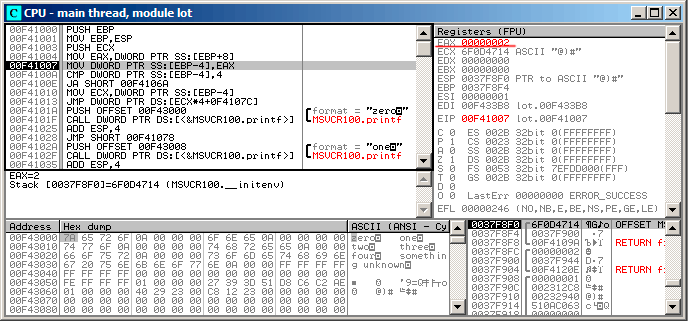
\includegraphics[scale=\FigScale]{patterns/08_switch/2_lot/lot_olly1.png}
\caption{\olly: \RU{входное значение ф-ции загружено в}\EN{function's input value is loaded in} \EAX}
\label{fig:switch_lot_olly1}
\end{figure}

\begin{figure}[H]
\centering
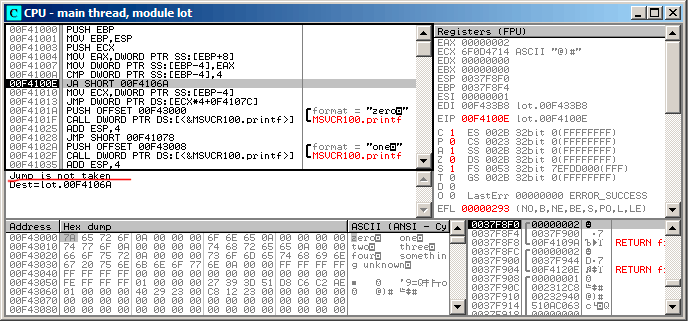
\includegraphics[scale=\FigScale]{patterns/08_switch/2_lot/lot_olly2.png}
\caption{\olly: $2$ \RU{не больше чем}\EN{is no bigger than} $4$: \RU{переход не сработает}\EN{no jump is taken}}
\label{fig:switch_lot_olly2}
\end{figure}

\begin{figure}[H]
\centering
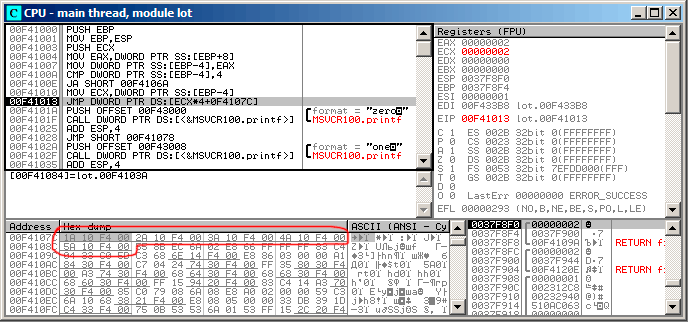
\includegraphics[scale=\FigScale]{patterns/08_switch/2_lot/lot_olly3.png}
\caption{\olly: \RU{вычисляем адрес для перехода используя}\EN{calculating destination address using} jumptable}
\label{fig:switch_lot_olly3}
\end{figure}

\begin{figure}[H]
\centering
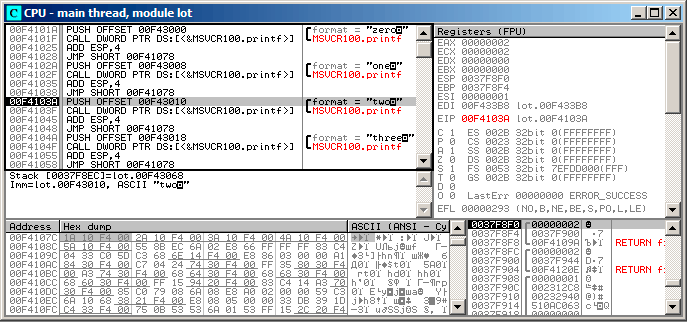
\includegraphics[scale=\FigScale]{patterns/08_switch/2_lot/lot_olly4.png}
\caption{\olly: \RU{теперь мы на соответствующей метке}\EN{now we at corresponding} \IT{case:}\EN{ label}}
\label{fig:switch_lot_olly4}
\end{figure}
\fi

\subsubsection{\NonOptimizing GCC}
\label{switch_lot_GCC}

\RU{Посмотрим, что сгенерирует GCC 4.4.1}\EN{Let's see what GCC 4.4.1 generates}:

\lstinputlisting[caption=GCC 4.4.1]{patterns/08_switch/2_lot/lot_gcc.asm}

\index{x86!\Registers!JMP}
\RU{Практически то же самое, за исключением мелкого нюанса: аргумент из \TT{arg\_0} умножается на 4 
при помощи сдвига влево на 2 бита (это почти то же самое что и умножение на 4)~(\ref{SHR}).
Затем адрес метки внутри функции берется из массива \TT{off\_804855C} и адресуется при помощи 
вычисленного индекса.}
\EN{It is almost the same, except little nuance: argument \TT{arg\_0} is multiplied by 4 by
shifting it to left by 2 bits (it is almost the same as multiplication by 4)~(\ref{SHR}).
Then label address is taken from \TT{off\_804855C} array, address is calculated and stored into 
\EAX, then \TT{``JMP EAX''} do actual jump.}


\ifdefined\IncludeARM
\subsection{ARM: \OptimizingKeilVI (\ARMMode)}
\label{sec:SwitchARMLot}

\lstinputlisting[caption=\OptimizingKeilVI (\ARMMode)]{patterns/08_switch/2_lot/lot_ARM_ARM_O3.asm}

\RU{В этом коде используется та особенность режима ARM, 
что все инструкции в этом режиме имеют фиксированную длину 4 байта.}
\EN{This code makes use of the ARM mode feature in which all instructions have a fixed size of 4 bytes.}

\RU{Итак, не будем забывать, что максимальное значение для $a$ это $4$, всё что выше, должно вызвать
вывод строки}
\EN{Let's keep in mind that the maximum value for $a$ is $4$ and any greater value will cause}
\IT{<<something unknown\textbackslash{}n>>}
\RU{.}\EN{to string printing.}

\index{ARM!\Instructions!CMP}
\index{ARM!\Instructions!ADDCC}
\RU{Самая первая инструкция}\EN{The first} \TT{``CMP R0, \#5''} 
\RU{сравнивает входное значение в $a$ c $5$.}
\EN{instruction compares the input value of $a$ with $5$.}

\RU{Следующая инструкция}\EN{The next} \TT{``ADDCC PC, PC, R0,LSL\#2''}
\footnote{ADD\EMDASH\RU{складывание чисел}\EN{addition}}
\RU{сработает только в случае если}\EN{instruction will execute only if} $R0 < 5$ (\IT{CC=Carry clear / Less than}). 
\RU{Следовательно, если}\EN{Consequently, if} \TT{ADDCC} \RU{не сработает}\EN{does not trigger} 
(\RU{это случай с}\EN{it is a} $R0 \geq 5$\EN{ case}), 
\RU{выполнится переход на метку}\EN{a jump to} 
\IT{default\_case}\RU{.}\EN{ label will occur.}

\RU{Но если}\EN{But if} $R0 < 5$ \AndENRU \TT{ADDCC} \RU{сработает, то произойдет следующее:}
\EN{triggers, the following will happen:}

\RU{Значение в \Reg{0} умножается на $4$}\EN{The value in \Reg{0} will be multiplied by $4$}.
\RU{Фактически}\EN{In fact}, \TT{LSL\#2} \RU{в суффиксе инструкции означает ``сдвиг влево на 2 бита''.}
\EN{at the instruction's suffix means ``shift left by 2 bits''.}
\RU{Но как будет видно позже}\EN{But as we will see later}~(\myref{division_by_shifting}) \RU{в секции}\EN{in section} 
``\ShiftsSectionName'', 
\RU{сдвиг влево на 2 бита это как раз эквивалентно его умножению на $4$.}
\EN{shift left by 2 bits is equivalent to multiplying by $4$.}

\RU{Затем полученное}\EN{Then we add} $R0*4$ \RU{прибавляется к текущему значению \ac{PC}}\EN{to
the current value in \ac{PC}}, 
\RU{совершая, таким образом, переход на одну из расположенных ниже инструкций \TT{B} (\IT{Branch}).}
\EN{thus jumping to one of the \TT{B} (\IT{Branch}) instructions located below.}

\RU{На момент исполнения}\EN{At the moment of the execution of} \TT{ADDCC},
\RU{содержимое \ac{PC} на 8 байт больше}\EN{the value in \ac{PC} is 8 bytes ahead} (\TT{0x180}) 
\RU{чем адрес по которому расположена сама инструкция} 
\EN{than the address at which the} \TT{ADDCC}\EN{ instruction is located} (\TT{0x178}), 
\RU{либо, говоря иным языком, на 2 инструкции больше.}
\EN{or, in other words, 2 instructions ahead.}

\index{ARM!\RU{Конвейер}\EN{Pipeline}}
\RU{Это связано с работой конвейера процессора ARM:
пока исполняется инструкция \TT{ADDCC}, процессор уже начинает обрабатывать инструкцию после следующей, 
поэтому \ac{PC} указывает туда. Этот факт нужно запомнить.}
\EN{This is how the pipeline in ARM processors works: when \TT{ADDCC} is executed,
the processor at the moment
is beginning to process the instruction after the next one,
so that is why \ac{PC} points there. This should be memorized.}

\RU{В случае, если $a=0$, тогда к \ac{PC} ничего не будет прибавлено, 
в \ac{PC} запишется актуальный на тот момент \ac{PC} (который больше на 8) 
и произойдет переход на метку \IT{loc\_180}, 
это на 8 байт дальше от места где находится инструкция \TT{ADDCC}.}
\EN{If $a=0$, then nothing will be added to the value in \ac{PC},
and the actual value in the \ac{PC} will be written into \ac{PC} (which is 8 bytes ahead)
and a jump to the label \IT{loc\_180} will happen,
which is 8 bytes ahead of the point where the \TT{ADDCC} instruction is.}

\RU{В случае, если}\EN{If} $a=1$, \RU{тогда в \ac{PC} запишется}\EN{then} 
$PC+8+a*4 = PC+8+1*4 = PC+12 = 0x184$\RU{, это адрес метки \IT{loc\_184}}\EN{ will be written to \ac{PC},
which is the address of the \IT{loc\_184} label}.

\RU{При каждой добавленной к $a$ единице, итоговый \ac{PC} увеличивается на $4$.}
\EN{With every $1$ added to $a$, the resulting \ac{PC} is increased by $4$.}
\RU{$4$ это как раз длина инструкции  в режиме ARM и одновременно с этим, 
длина каждой инструкции \TT{B}, их здесь следует 5 в ряд.}
\EN{$4$ is the instruction length in ARM mode and also, the length of each \TT{B} instruction,
of which there are 5 in row.}

\RU{Каждая из этих пяти инструкций \TT{B}, передает управление дальше, где собственно и происходит то, 
что запрограммировано в}
\EN{Each of these five \TT{B} instructions passes control further, to 
what was programmed in the}
\IT{switch()}.
\RU{Там происходит загрузка указателя на свою строку, и т.д.}
\EN{Pointer loading of the corresponding string occurs there, etc.}

\subsection{ARM: \OptimizingKeilVI (\ThumbMode)}

\lstinputlisting[caption=\OptimizingKeilVI (\ThumbMode)]{patterns/08_switch/2_lot/lot_ARM_thumb_O3.asm}

\index{ARM!\ThumbMode}
\index{ARM!\ThumbTwoMode}
\RU{В режимах thumb и thumb-2, уже нельзя надеяться на то что все инструкции будут иметь одну длину.}
\EN{One cannot be sure that all instructions in thumb and thumb-2 modes will have the same size.}
\RU{Можно даже сказать, что в этих режимах инструкции переменной длины, как в x86.}
\EN{It can even be said that in these modes the instructions have variable lengths, just like in x86.}

\index{jumptable}
\RU{Так что здесь добавляется специальная таблица, содержащая информацию о том, как много вариантов здесь,
не включая default-варианта, и смещения, для каждого варианта, каждое кодирует метку, куда нужно передать
управление в соответствующем случае.}
\EN{So there is a special table added that contains information about how much cases are there (not including 
default-case), and an offset for each with a label to which control must be passed in 
the corresponding case.}

\index{ARM!\RU{Переключение режимов}\EN{Mode switching}}
\index{ARM!\Instructions!BX}
\RU{Для того чтобы работать с таблицей и совершить переход, вызывается служебная функция}
\EN{A special function is present here in order to deal with the table and pass control, named} \\
\IT{\_\_ARM\_common\_switch8\_thumb}. 
\RU{Она начинается с инструкции}\EN{It starts with} \TT{``BX PC''}
\RU{, чья функция ~--- переключить процессор в ARM-режим.}
\EN{, whose function is to switch the processor to ARM-mode.}
\RU{Далее функция, работающая с таблицей.}\EN{Then you see the function for table processing.} 
\RU{Она слишком сложная для 
рассмотрения в данном месте, так что я пропущу все объяснения.}
\EN{It is too complex to describe it here now, so I will omit it.}
% TODO дописать когда-то?

\index{ARM!\Registers!Link Register}
\RU{Но можно отметить, что эта функция использует регистр \ac{LR} как указатель на таблицу.}
\EN{It is interesting to note that the function uses the \ac{LR} register as a pointer to the table.}
\RU{Действительно, после вызова этой функции, в \ac{LR} был записан
адрес после инструкции}\EN{Indeed, after this calling this function, \ac{LR} will contain the address after} \\ 
\TT{``BL \_\_ARM\_common\_switch8\_thumb''}\RU{, а там как раз и начинается таблица.}
\EN{ instruction, where the table starts.}

\RU{Еще можно отметить что код для этого выделен в отдельную функцию для того, 
чтобы не нужно было каждый раз генерировать 
точно такой же фрагмент кода для каждого выражения switch().}
\EN{It is also worth noting that the code is generated as a separate function in order to reuse it, 
so the compiler will not generate the same code for every switch() statement.}

\IDA 
\RU{распознала эту служебную функцию и таблицу автоматически, дописав комментарии к меткам вроде}
\EN{successfully perceived it as a service function and a table, and added comments to the labels
like}\\
\TT{jumptable 000000FA case 0}.


\fi
\ifdefined\IncludeMIPS
\subsection{MIPS}

\lstinputlisting[caption=\Optimizing GCC 4.4.5 (IDA)]{patterns/08_switch/2_lot/MIPS_O3_IDA.lst.\LANG}

\index{MIPS!\Instructions!SLTIU}
\RU{Новая для нас инструкция здесь это SLTIU (``Set on Less Than Immediate Unsigned''~--- установить,
если меньше чем значение, беззнаковое сравнение).}
\EN{The new instruction for us is SLTIU (``Set on Less Than Immediate Unsigned'').}
\index{MIPS!\Instructions!SLTU}
\RU{На самом деле, это то же что и SLTU (``Set on Less Than Unsigned''), но ``I'' означает ``immediate'',
т.е. число может быть задано в самой инструкции.}
\EN{This is the same as SLTU (``Set on Less Than Unsigned''), but ``I'' stands for ``immediate'', 
i.e., a number has to be specified in the instruction itself.}

\index{MIPS!\Instructions!BNEZ}
BNEZ \RU{это}\EN{is} ``Branch if Not Equal to Zero''\RU{ (переход если не равно нулю)}.

\RU{Код очень похож на код для других \ac{ISA}.}\EN{Code is very close to the other \ac{ISA}s.}
\index{MIPS!\Instructions!SLL}
SLL (``Shift Word Left Logical''\RU{~--- логический сдвиг влево}) 
\RU{совершает умножение на 4}\EN{does multiplication by 4}.
\RU{MIPS всё-таки это 32-битный процессор, так что все адреса в таблице переходов 
(\IT{jumptable}) 32-битные.}
\EN{MIPS is a 32-bit CPU after all, so all addresses in the \IT{jumptable} are 32-bit ones.}

\fi

\subsection{\Conclusion{}}

\RU{Примерный скелет}\EN{Rough skeleton of} \IT{switch()}:

% TODO:  ARM, MIPS skeleton
\lstinputlisting[caption=x86]{patterns/08_switch/2_lot/skel1.lst.\LANG}

\RU{Переход по адресу из таблицы переходов может быть также реализован такой инструкцией:}
\EN{The jump to the address in the jump table may also be implemented using this instruction:}
\TT{JMP jump\_table[REG*4]}.
\RU{Или}\EN{Or} \TT{JMP jump\_table[REG*8]} \InENRU x64.

\RU{Таблица переходов (\IT{jumptable}) это просто массив указателей, как это будет вскоре описано:}
\EN{A \IT{jumptable} is just array of pointers, like the one described later:}
\ref{array_of_pointers_to_strings}.

\section{\RU{Когда много \IT{case} в одном блоке}
\EN{When there are several \IT{case} in one block}}

\RU{Вот очень часто используемая конструкция: несколько \IT{case} может быть использовано в одном блоке:}
\EN{Here is also a very often used construction: several \IT{case} statements may be used in single block:}

\lstinputlisting{patterns/08_switch/3_several_cases/several_cases.c}

\RU{Слишком расточительно генерировать каждый блок для каждого случая, поэтому обычно
каждый блок генерируется плюс диспетчер.}
\EN{It's too wasteful to generate each block for each possible case,
so what is usually done, is each block generated plus some kind of dispatcher.}

\subsection{MSVC}

\lstinputlisting[caption=\Optimizing MSVC 2010,numbers=left]{patterns/08_switch/3_several_cases/several_cases_MSVC_2010_Ox.asm.\LANG}

\RU{Здесь видим две таблицы}\EN{We see two tables here}: 
\RU{первая таблица}\EN{the first table} (\TT{\$LN10@f}) \RU{это таблица индексов}\EN{is index table},
\RU{и вторая таблица}\EN{and the second table} (\TT{\$LN11@f}) \RU{это массив указателей на блоки}\EN{is 
an array of pointers to blocks}.

\RU{В начале, входное значение используется как индекс в таблице индексов}\EN{First, input value 
is used as index in index table} (\LineENRU 13). 

\RU{Вот краткое описание значений в таблице}\EN{Here is short legend for values in the table}: 
0 \RU{это первый блок \IT{case}}\EN{is first \IT{case} block} (\RU{для значений}\EN{for values} 1, 2, 7, 10),
1 \RU{это второй}\EN{is second} (\RU{для значений}\EN{for values} 3, 4, 5),
2 \RU{это третий}\EN{is third} (\RU{для значений}\EN{for values} 8, 9, 21),
3 \RU{это четвертый}\EN{is fourth} (\RU{для значений}\EN{for value} 22),
4 \RU{это для default-блока}\EN{is for default block}.

\RU{Мы получаем индекс для второй таблицы указателей на блоки и переходим туда}\EN{We get there index for 
the second table of block pointers and we jump there} (\LineENRU 14).

\EN{What is also worth to note that there are no case for input value $0$.}
\RU{Что еще нужно отметить, так это то что здесь нет случая для нулевого входного значения.}
\EN{Hence, we see \DEC instruction at line 10, and the table is beginning at $a=1$. 
Because there are no need to allocate table element for $a=0$.}
\RU{Поэтому мы видим инструкцию \DEC на строке 10 и таблица начинается с $a=1$.
Потому что незачем выделять в таблице элемент для $a=0$.}

\RU{Это очень часто используемый шаблон}\EN{This is very often used pattern}.

\RU{В чем же экономия}\EN{So where economy is}?
\RU{Почему нельзя сделать так, как уже обсуждалось}\EN{Why it's not possible to make it as it was 
already discussed} (\ref{switch_lot_GCC}), \RU{используя только одну таблицу, содержащую указатели на 
блоки}\EN{just with one table, consisting of block pointers}?
\RU{Причина в том, что элементы в таблице индексов занимают только по 8-битному байту, поэтому всё это более 
компактно}\EN{The reason is that elements in index table has 8-bit byte type, hence it's all more compact}.

\subsection{GCC}

GCC \RU{делает так, как уже обсуждалось}\EN{do the job like it was already discussed} 
(\ref{switch_lot_GCC}), \RU{используя просто таблицу указателей}\EN{using just one table of pointers}.

\subsection{ARM64: \Optimizing GCC 4.9.1}

\RU{Во-первых, здесь нет кода, срабатывающего в случае если входное значение --- 0, так что GCC пытается
сделать таблицу переходов более компактной и начинает с случая, когда входное значение --- 1.}
\EN{First of all, there are no code triggering if input value is 0, so GCC tries to make jumptable more compact
and so it's started at the case of 1 as input value.}

GCC 4.9.1 \ForENRU ARM64 \RU{использует даже более интересный трюк}\EN{uses even cleverer trick}.
\RU{Он может закодировать все смещения как 8-битные байты}\EN{It's able to encode all offsets as 8-bit bytes}.
\RU{Вспомним что все инструкции в ARM64 имеют размер в 4 байта.}
\EN{Let's remind ourselves, all ARM64 instructions has size of 4 bytes.}
\RU{GCC также использует тот факт, что все смещения в моем крохотном примере находятся достаточно близко 
друг от друга.}
\EN{GCC is also use the fact that all offsets in my tiny example are in close proximity to each other.}
\RU{Так что таблица переходов состоит из байт.}\EN{So the jumptable consisting of bytes.}

\lstinputlisting[caption=\Optimizing GCC 4.9.1 ARM64]{patterns/08_switch/3_several_cases/ARM64_GCC491_O3.s.\LANG}

\RU{Я скомпилировал мой пример как объектный файл и открыл его в IDA. Вот таблица переходов:}
\EN{I just compiled my example to object file and opened it in IDA. Here is a jump table:}

\lstinputlisting[caption=jumptable in IDA]{patterns/08_switch/3_several_cases/ARM64_GCC491_O3_IDA.lst}

\RU{В случае 1, 9 будет умножено на 9 и прибавлено к адресу метки Lrtx4.}
\EN{So in case of 1, 9 will be multiplied by 4 and added to the address of Lrtx4 label.}
\RU{В случае 22, 0 будет умножено на 4, в результате это 0.}
\EN{In case of 22, 0 is to be multiplied by 4 resulting 0. }
\RU{Место сразу за меткой Lrtx4, это метка L7, где находится код выводящий ``22''.}
\EN{The place right after Lrtx4 label is L7 label, where the code printing ``22'' is.}
\RU{В сегменте кода нет таблицы переходов, место для нее выделено в отдельной секции .rodata
(нет особой нужды располагать её в сегменте кода).}
\EN{There are no jumptable in the code segment, a place for it is allocated in separate .rodata section 
(there are no special need to place it in code section).}

\RU{Там есть также отрицательные байты (0xF7), они используются для перехода назад, на код выводящий
строку ``default'' (на .L2).}
\EN{There are also negative bytes (0xF7), they are used for jumping back to the code printing ``default'' string 
(at .L2).}

\section{Fall-through}

\RU{Еще одно популярное использование}\EN{Another very popular usage of} \TT{switch()} 
\EN{is the fall-through}\RU{это т.н. ``fallthrough'' (``проваливаясь'')}.
\RU{Вот простой пример}\EN{Here is a small example}:

\lstinputlisting[numbers=left]{patterns/08_switch/4_fallthrough/fallthrough.c}

\RU{Если}\EN{If} $type=1$ (R), $read$ \RU{будет выставлен в}\EN{will be set to} $1$, \RU{если}\EN{if} 
$type=2$ (W), $write$ \RU{будет выставлен в}\EN{will be set to} $2$.
\RU{В случае}\EN{In case of} $type=3$ (RW), \RU{обе}\EN{both} $read$ \AndENRU $write$ \RU{будут 
выставлены в}\EN{will be set to} $1$.

\RU{Фрагмент кода на строке 14 будет исполнен в двух случаях: если}\EN{The code at 
line 14 is executed in two cases: if} $type=RW$ \RU{или если}\EN{or if} $type=W$.
\RU{Там нет ``break'' для ``case RW'', и это нормально}\EN{There is no ``break'' 
for ``case RW''x and that's OK}.

\subsection{MSVC x86}

\lstinputlisting[caption=MSVC 2012]{patterns/08_switch/4_fallthrough/fallthrough_MSVC.asm}

\RU{Код почти полностью повторяет то что в исходнике.}
\EN{The code mostly resembles what is in the source.}
\RU{Там нет переходов между метками}\EN{There are no jumps between labels} \TT{\$LN4@f} \AndENRU 
\TT{\$LN3@f}: \RU{так что когда управление (code flow) находится на}\EN{so when code flow is at} 
\TT{\$LN4@f}, $read$ \RU{в начале выставляется в $1$, затем}\EN{is first set to $1$, then} $write$.
\EN{This is why it's called fall-through: code flow falls through one piece of code
(setting $read$) to another (setting $write$).}
\RU{Наверное, поэтому всё это и называется ``проваливаться'': управление проваливается через
один фрагмент кода (выставляющий $read$) в другой (выставляющий $write$).}
\RU{Если}\EN{If} $type=W$, \RU{мы оказываемся на}\EN{we land at} \TT{\$LN3@f}, 
\RU{так что код выставляющий $read$ в $1$ не исполнится}\EN{so no code setting $read$ to $1$ 
is executed}.

\ifdefined\IncludeARM
\subsection{ARM64}

\lstinputlisting[caption=GCC (Linaro) 4.9]{patterns/08_switch/4_fallthrough/fallthrough_ARM64.s.\LANG}

\RU{Почти то же самое}\EN{Merely the same thing}.
\RU{Здесь нет переходов между метками}\EN{There are no jumps between labels} \TT{.L4} 
\AndENRU \TT{.L3}.
\fi


\ifdefined\IncludeExercises
\section{\Exercises}

\subsection{\Exercise \#1}
\label{exercise_switch_1}

\RU{Вполне возможно переделать пример на Си в листинге \ref{switch_lot_c} так, чтобы при компиляции
получалось даже еще меньше кода, но работать всё будет точно так же.}
\EN{It's possible to rework C example in \ref{switch_lot_c} in such way, so the compiler
will produce even smaller code, but it will work just the same.}
\RU{Попробуйте этого добиться}\EN{Try to achieve it}.

\RU{Подсказка}\EN{Hint}: \ref{exercise_solutions_switch_1}.
\fi

\chapter{\Loops}
\label{sec:loops}

% sections
\subsection{\RU{Простой пример}\EN{Simple example}}

% subsubsections
\subsection{x86}

\index{x86!\Instructions!LOOP}
\RU{Для организации циклов в архитектуре x86 есть старая инструкция \LOOP. 
Она проверяет значение регистра \ECX и если оно не 0, делает \glslink{decrement}{декремент} \ECX 
и переход по метке, указанной в операнде. 
Возможно, эта инструкция не слишком удобная, потому что уже почти не бывает современных компиляторов, 
которые использовали бы её. Так что если вы видите где-то \LOOP, то с большой вероятностью это 
вручную написанный код на ассемблере.}
\EN{There is a special \LOOP instruction in x86 instruction set for checking the value in register \ECX and 
if it is not 0, to \gls{decrement} \ECX
and pass control flow to the label in the \LOOP operand. 
Probably this instruction is not very convenient, and there are no any modern compilers which emit it automatically.
So, if you see this instruction somewhere in code, it is most likely that this is a manually written piece 
of assembly code.}\PTBRph{}\ESph{}\PLph{}\\
\\
\RU{Обычно, циклы на \CCpp создаются при помощи \TT{for()}, \TT{while()}, \TT{do/while()}.}
\EN{In \CCpp loops are usually constructed using \TT{for()}, \TT{while()} or \TT{do/while()} statements.}

\RU{Начнем с}\EN{Let's start with} \TT{for()}.
\index{\CLanguageElements!for}

\RU{Это выражение описывает инициализацию, условие, операцию после каждой итерации
(\glslink{increment}{инкремент}/\glslink{decrement}{декремент})
и тело цикла.}
\EN{This statement defines loop initialization (set loop counter to initial value), 
loop condition (is the counter bigger than a limit?), what is done at each iteration (\gls{increment}/\gls{decrement})
and of course loop body.}

\lstinputlisting{patterns/09_loops/simple/loops_1.c.\LANG}

\RU{Примерно так же, генерируемый код и будет состоять из этих четырех частей.}
\EN{The generated code is consisting of four parts as well.}

\RU{Возьмем пример}\EN{Let's start with a simple example}:

\lstinputlisting[label=loops_src]{patterns/09_loops/simple/loops_2.c}

\RU{Имеем в итоге}\EN{Result} (MSVC 2010):

\lstinputlisting[caption=MSVC 2010]{patterns/09_loops/simple/1_MSVC.asm.\LANG}

\RU{В принципе, ничего необычного.}\EN{As we see, nothing special.}

\ifdefined\IncludeGCC
\RU{GCC 4.4.1 выдает примерно такой же код, с небольшой разницей:}
\EN{GCC 4.4.1 emits almost the same code, with one subtle difference:}

\lstinputlisting[caption=GCC 4.4.1]{patterns/09_loops/simple/1_GCC.asm.\LANG}

\RU{Интересно становится, если скомпилируем этот же код при помощи MSVC 2010 с включенной оптимизацией}
\EN{Now let's see what we get with optimization turned on} (\Ox):
\fi

\lstinputlisting[caption=\Optimizing MSVC]{patterns/09_loops/simple/1_MSVC_Ox.asm}

\RU{Здесь происходит следующее: переменную $i$ компилятор не выделяет в локальном стеке, 
а выделяет целый регистр под нее: \ESI. 
Это возможно для маленьких функций, где мало локальных переменных.}
\EN{What happens here is that space for the $i$ variable is not allocated in the local stack anymore,
but uses an individual register for it, \ESI.
This is possible in such small functions where there aren't many local variables.}

\RU{В принципе, всё то же самое, только теперь одна важная особенность: 
\ttf не должна менять значение \ESI. 
Наш компилятор уверен в этом, а если бы и была необходимость использовать регистр \ESI в функции \ttf, 
то её значение сохранялось бы в стеке. Примерно так же как и в нашем листинге: 
обратите внимание на \TT{PUSH ESI/POP ESI} в начале и конце функции.}
\EN{One very important thing is that the \ttf function must not change the value in \ESI.
Our compiler is sure here. 
And if the compiler decides to use the \ESI register in \ttf too, its value would have to be saved 
at the function's prologue and restored at the function's epilogue,
almost like in our listing: please note \TT{PUSH ESI/POP ESI}
at the function start and end.}

\ifdefined\IncludeGCC
\RU{Попробуем GCC 4.4.1 с максимальной оптимизацией (\Othree):}
\EN{Let's try GCC 4.4.1 with maximal optimization turned on (\Othree option):}

\lstinputlisting[caption=\Optimizing GCC 4.4.1]{patterns/09_loops/simple/1_GCC_O3.asm}

\index{Loop unwinding}
\RU{Однако GCC просто \IT{развернул} цикл\footnote{\gls{loop unwinding} в англоязычной литературе}.}
\EN{Huh, GCC just unwound our loop.}

\RU{Делается это в тех случаях, когда итераций не слишком много (как в нашем примере)
и можно немного сэкономить время, убрав все инструкции, обеспечивающие цикл. 
В качестве обратной стороны медали, размер кода увеличился.}
\EN{\Gls{loop unwinding} has an advantage in the cases when there aren't much iterations and 
we could cut some execution time by removing all loop support instructions. 
On the other side, the resulting code is obviously larger.}

\EN{Big unrolled loops are not recommended in modern times, because bigger functions
may require bigger cache footprint}%
\RU{Использовать большие развернутые циклы в наше время не рекомендуется, потому что большие
функции требуют больше кэш-памяти}%
\footnote{
\EN{A very good article about it}\RU{Очень хорошая статья об этом}: \cite{DrepperMemory}.
\EN{Another recommendations about loop unrolling from Intel are here}
\RU{А также о рекомендациях о развернутых циклах от Intel можно прочитать здесь}: 
\cite[3.4.1.7]{IntelOptimization}.}.\\
\\
\RU{Увеличим максимальное значение $i$ в цикле до 100 и попробуем снова. GCC выдает:}
\EN{OK, let's increase the maximum value of the $i$ variable to 100 and try again. GCC does:}

\lstinputlisting[caption=GCC]{patterns/09_loops/simple/2_GCC.asm.\LANG}

\RU{Это уже похоже на то, что сделал MSVC 2010 в режиме оптимизации (\Ox). 
За исключением того, что под переменную $i$ будет выделен регистр \EBX.}
\EN{It is quite similar to what MSVC 2010 with optimization (\Ox) produce, 
with the exception that the \EBX register is allocated for the $i$ variable.}
\RU{GCC уверен, что этот регистр не будет 
модифицироваться внутри \ttf, а если вдруг это и придётся там сделать, то его значение будет сохранено 
в начале функции, прямо как в \main.}
\EN{GCC is sure this register will not be modified inside of the \ttf function, 
and if it will, it will be saved at the function prologue and restored at epilogue, 
just like here in the \main function.}
\fi

\ifdefined\IncludeOlly
\clearpage
\subsection{x86: \olly}
\index{\olly}

\RU{Скомпилируем наш пример в}\EN{Let's compile our example in} MSVC 2010 \RU{с}\EN{with} \Ox \AndENRU \Obzero 
\RU{и загрузим в}\EN{options and load it into} \olly.

\RU{Оказывается,}\EN{It seems that} \olly \RU{может обнаруживать простые циклы и показывать их в квадратных скобках, 
для удобства}\EN{is able to detect simple loops and show them in square brackets, for convenience}:

\begin{figure}[H]
\centering
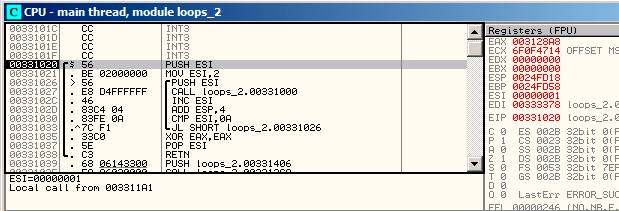
\includegraphics[scale=\FigScale]{patterns/09_loops/simple/olly1.png}
\caption{\olly: \RU{начало \main}\EN{\main begin}}
\label{fig:loops_olly_1}
\end{figure}

\RU{Трассируя}\EN{By tracing} (F8~--- \stepover) \RU{мы видим, как}\EN{we see} \ESI \RU{увеличивается на 1.}
\EN{\glslink{increment}{incrementing}.}
\RU{Например, здесь}\EN{Here, for instance,} $ESI=i=6$:

\begin{figure}[H]
\centering
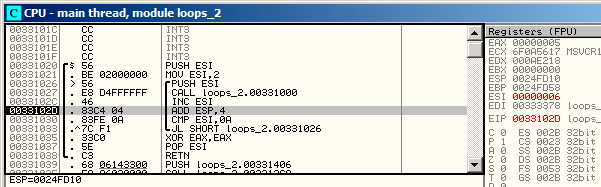
\includegraphics[scale=\FigScale]{patterns/09_loops/simple/olly2.png}
\caption{\olly: \RU{тело цикла только что отработало с}\EN{loop body just executed with} $i=6$}
\label{fig:loops_olly_2}
\end{figure}

9 \RU{это последнее значение цикла}\EN{is the last loop value}.
\RU{Поэтому}\EN{That's why} \JL 
\RU{после \glslink{increment}{инкремента} не срабатывает и функция заканчивается:}
\EN{is not triggering after the \gls{increment}, and the function will finish:}

\begin{figure}[H]
\centering
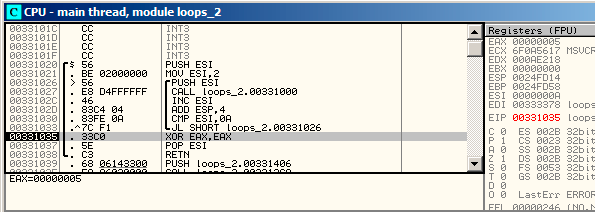
\includegraphics[scale=\FigScale]{patterns/09_loops/simple/olly3.png}
\caption{\olly: $ESI=10$, \RU{конец цикла}\EN{loop end}}
\label{fig:loops_olly_3}
\end{figure}

\subsection{x86: tracer}
\index{tracer}

\RU{Как видно, трассировать вручную цикл в отладчике\EMDASH{}это не очень удобно.}%
\EN{As we might see, it is not very convenient to trace manulally in the debugger.}
\RU{Поэтому попробуем \tracer.}%
\EN{That's a reason we will try \tracer.}

\RU{Открываем скомпилированный пример в \IDA, находим там адрес инструкции \INS{PUSH ESI}
(передающей единственный аргумент в \ttf,)
а это \TT{0x401026} в нашем случае и запускаем \tracer:}
\EN{We open compiled example in \IDA, find the address of the instruction \INS{PUSH ESI}
(passing the sole argument to \ttf,) which is \TT{0x401026} for this case and we run the \tracer:}

\begin{lstlisting}
tracer.exe -l:loops_2.exe bpx=loops_2.exe!0x00401026
\end{lstlisting}

\RU{Опция }\TT{BPX} 
\RU{просто ставит точку останова по адресу и затем tracer будет выдавать состояние регистров.}
\EN{just sets a breakpoint at the address and tracer will then print the state of the registers.}

\RU{В}\EN{In the} \TT{tracer.log} \RU{после запуска я вижу следующее}\EN{This is what we see}:

\lstinputlisting{patterns/09_loops/simple/tracer.log}

\RU{Видно, как значение}\EN{We see how the value of} \ESI \RU{последовательно изменяется от 2 до 9.}
\EN{register changes from 2 to 9.}

\RU{И даже более того, в \tracer можно собирать значения регистров по всем адресам внутри функции.}
\EN{Even more than that, the \tracer can collect register values for all addresses within the function.}
\RU{Там это называется}\EN{This is called} \IT{trace}\EN{ there}.
\RU{Каждая инструкция трассируется, значения самых интересных регистров запоминаются}\EN{Every instruction
gets traced, all interesting register values are recorded}.
\RU{Затем генерируется .idc-скрипт для \IDA, который добавляет комментарии.}
\EN{Then, an \IDA .idc-script is generated, that adds comments.}
\RU{Итак, в}\EN{So, in the} \IDA \RU{я узнал что адрес}\EN{we've learned that the} \main \RU{это}\EN{function address
is} \TT{0x00401020} \RU{и запускаю}\EN{and we run}:

\begin{lstlisting}
tracer.exe -l:loops_2.exe bpf=loops_2.exe!0x00401020,trace:cc
\end{lstlisting}

\TT{BPF} \RU{означает установить точку останова на функции}\EN{stands for set breakpoint on function}.

\RU{Получаю в итоге скрипты}\EN{As a result, we get the} \TT{loops\_2.exe.idc} \AndENRU 
\TT{loops\_2.exe\_clear.idc}\EN{ scripts}.

\clearpage
\RU{Загружаю}\EN{We load} \TT{loops\_2.exe.idc} \RU{в}\EN{into} \IDA \RU{и увижу следующее}\EN{and see}:

\begin{figure}[H]
\centering
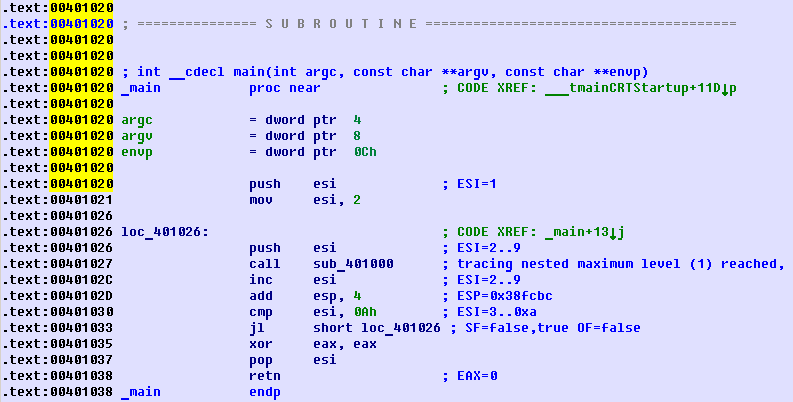
\includegraphics[scale=\FigScale]{patterns/09_loops/simple/IDA_tracer_cc.png}
\caption{\IDA \RU{с загруженным .idc-скриптом}\EN{with .idc-script loaded}}
\label{fig:loops_IDA_tracer}
\end{figure}

\RU{Видно, что}\EN{We see that} \ESI \RU{меняется от 2 до 9 в начале тела цикла, но после 
\glslink{increment}{инкремента} он в пределах [3..0xA]}\EN{can be from 2 to 9 at the start of the loop body,
but from 3 to 0xA (10) after the increment}.
\RU{Видно также, что функция}\EN{We can also see that} \main \RU{заканчивается с 0 в}\EN{is finishing with 0 in} \EAX.

\tracer \RU{также генерирует}\EN{also generates} \TT{loops\_2.exe.txt}, 
\RU{содержащий адреса инструкций, сколько раз была исполнена
каждая и значения регистров}\EN{that contains information about how many times each instruction was executed and
register values}:

\lstinputlisting[caption=loops\_2.exe.txt]{patterns/09_loops/simple/loops_2.exe.txt}
\index{\GrepUsage}
\RU{Так можно использовать grep}\EN{We can use grep here}.

\fi

\subsubsection{ARM: \NonOptimizingKeilVI (\ARMMode)}

\lstinputlisting[label=Keil_number_sign]{patterns/09_loops/simple/Keil_ARM_O0.asm}

\RU{Счетчик итераций $i$ будет храниться в регистре \Reg{4}.}
\EN{Iteration counter $i$ is to be stored in the \Reg{4} register.}

\RU{Инструкция }\TT{``MOV R4, \#2''} \RU{просто инициализирует}\EN{instruction just initializing} $i$.

\RU{Инструкции }\TT{``MOV R0, R4''} \AndENRU \TT{``BL f''} \RU{составляют тело цикла}\EN{instructions are
compose loop body}, 
\RU{первая инструкция готовит аргумент для функции \ttf и вторая собственно вызывает её.}
\EN{the first instruction preparing argument for \ttf function and the second is calling it.}

\index{ARM!\Instructions!ADD}
\RU{Инструкция }\TT{``ADD R4, R4, \#1''} \RU{прибавляет единицу к $i$ при каждой итерации.}
\EN{instruction is just adding $1$ to the $i$ variable during each iteration.}

\index{ARM!\Instructions!CMP}
\index{ARM!\Instructions!BLT}
\TT{``CMP R4, \#0xA''} \RU{сравнивает}\EN{comparing} $i$ \RU{с}\EN{with} \TT{0xA} ($10$). 
\RU{Следующая за ней инструкция}\EN{Next instruction} \TT{BLT} (\IT{Branch Less Than}) 
\RU{совершит переход, если}\EN{will jump if} $i$ \RU{меньше чем}\EN{is less than} $10$.

\RU{В противном случае}\EN{Otherwise}, \RU{в \Reg{0} запишется $0$}\EN{$0$ will be written into \Reg{0}} 
(\RU{потому что наша функция возвращает}\EN{since our function returns} $0$) 
\RU{и произойдет выход из функции}\EN{and function execution ended}.

\subsubsection{ARM: \OptimizingKeilVI (\ThumbMode)}

\lstinputlisting{patterns/09_loops/simple/Keil_thumb_O3.asm}

\RU{Практически, всё то же самое.}\EN{Practically, the same.}

\subsubsection{ARM: \OptimizingXcodeIV (\ThumbTwoMode)}
\label{ARM_unrolled_loops}

\lstinputlisting{patterns/09_loops/simple/xcode_thumb_O3.asm}

\RU{На самом деле, в моей функции \ttf было такое:}\EN{In fact, this was in my \ttf function:}

\begin{lstlisting}
void f(int i)
{
    // do something here
    printf ("%d\n", i);
};
\end{lstlisting}

\index{Unrolled loop}
\index{Inline code}
\RU{Так что}\EN{So}, LLVM \RU{не только \IT{развернул} цикл}\EN{not just \IT{unrolled} the loop}, 
\RU{но также и представил мою очень простую функцию \ttf как \IT{inline-вую}}\EN{but also represented my 
very simple function \ttf as \IT{inlined}},
\RU{и вставил её тело вместо цикла 8 раз}\EN{and inserted its body 8 times instead of loop}. 
\RU{Это возможно, когда функция очень простая, как та что у меня, и когда
она вызывается не очень много раз, как здесь.}
\EN{This is possible when function is so primitive (like mine) and when it is called not many times (like here).}



\subsubsection{\RU{Еще кое-что}\EN{One more thing}}

\RU{По генерируемому коду мы видим следующее}\EN{On the code generated we can see}: 
\RU{после инициализации}\EN{after} \IT{i}\RU{, тело цикла не исполняется, а исполняется сразу
проверка условия \IT{i}, а лишь затем исполняется тело цикла.}\EN{initialization, loop body will not be executed,
but \IT{i} condition checked first, and only after loop body is to be executed.}
\RU{Это правильно.}\EN{And that is correct.} 
\RU{Потому что если условие в самом начале не выполняется, тело цикла исполнять нельзя.}
\EN{Because, if loop condition is
not met at the beginning, loop body must not be executed.}
\RU{Так может быть, например, в таком случае:}\EN{For example, this is possible in the following case:}

\lstinputlisting{patterns/09_loops/simple/loops_3_\LANG.c}

\RU{Если}\EN{If} \IT{total\_entries\_to\_process} \RU{равно}\EN{equals to} $0$,
\RU{тело цикла не должно исполниться ни разу}\EN{loop body must not be executed whatsoever}.
\RU{Поэтому проверка условия происходит перед тем как исполнить само тело.}
\EN{So that is why condition checked before
loop body execution.}

\RU{Впрочем, оптимизирующий компилятор может переставить проверку условия и тело цикла местами, если он уверен,
что описанная здесь ситуация невозможна, как в случае с нашим простейшим примером и компиляторами 
Keil, Xcode (LLVM), MSVC и GCC в режиме оптимизации.}
\EN{However, optimizing compiler may swap condition check and loop body,
if it sure that the situation described here is
not possible (like in case of our very simple example and Keil, Xcode (LLVM), MSVC in optimization mode).}

\section{\RU{Функция копирования блоков памяти}\EN{Memory blocks copying routine}}
\label{loop_memcpy}

\RU{Настоящие ф-ции копирования памяти могут копировать по 4 или 8 байт на каждой итерации, использовать \ac{SIMD},
векторизацию, и т.д.}
\EN{Real-world memory copy routines may copy 4 or 8 bytes at each iteration, use \ac{SIMD}, 
vectorization, etc.}
\RU{Но ради простоты, этот пример настолько прост, насколько это возможно.}
\EN{But for the sake of simplicity, this example is the simplest possible.}

\lstinputlisting{memcpy.c}

\subsection{\RU{Простейшая реализация}\EN{Straight-forward implementation}}

\lstinputlisting[caption=GCC 4.9 x64 \RU{оптимизация по размеру}\EN{optimized for size} (-Os)]{patterns/09_loops/memcpy/memcpy_GCC49_x64_Os.s.\LANG}

\ifdefined\IncludeARM

\lstinputlisting[caption=GCC 4.9 ARM64 \RU{оптимизация по размеру}\EN{optimized for size} (-Os)]{patterns/09_loops/memcpy/memcpy_GCC49_ARM64_Os.s.\LANG}

\lstinputlisting[caption=\OptimizingKeilVI (\ThumbMode)]{patterns/09_loops/memcpy/memcpy_Keil_Thumb_O3.s.\LANG}

\subsection{ARM \RU{в режиме ARM}\EN{in ARM mode}}

\RU{Keil в режиме ARM пользуется условными суффиксами:}
\EN{Keil in ARM mode takes full advantage of conditional suffixes:}

\lstinputlisting[caption=\OptimizingKeilVI (\ARMMode)]{patterns/09_loops/memcpy/memcpy_Keil_ARM_O3.s.\LANG}

\RU{Вот почему здесь только одна инструкция перехода вместо двух.}
\EN{That's why there is only one branch instruction instead of 2.}

\fi

\ifdefined\IncludeMIPS
\subsection{MIPS}

\lstinputlisting[caption=GCC 4.4.5 \RU{оптимизация по размеру}\EN{optimized for size} (-Os) (IDA)]{patterns/09_loops/memcpy/memcpy_MIPS_Os_IDA.lst.\LANG}

\index{MIPS!\Instructions!LBU}
\index{MIPS!\Instructions!SB}
\RU{Здесь две новых для нас инструкций:}
\EN{Here we have two new instructions:} LBU (``Load Byte Unsigned'') \AndENRU SB (``Store Byte'').
\RU{Так же как и в ARM, все регистры в MIPS имеют длину в 32 бита, здесь нет частей регистров равных байту,
как в x86.}
\EN{Just like in ARM, all MIPS registers are 32-bit wide, there are no byte-wide parts like in x86.}
\RU{Так что, когда нужно работать с байтами, приходится выделять целый 32-битный регистр для этого.}
\EN{So when dealing with single bytes, we have to allocate whole 32-bit registers for them.}
\RU{LBU загружает байт и сбрасывает все остальные биты (``Unsigned'').}
\EN{LBU loads a byte and clears all other bits (``Unsigned'').}
\index{MIPS!\Instructions!LB}
\RU{И напротив, инструкция LB (``Load Byte'') расширяет байт до 32-битного значения учитывая знак.}
\EN{On the other hand, LB (``Load Byte'') instruction sign-extends the loaded byte to a 32-bit value.}
\RU{SB просто записывает байт из младших 8 бит регистра в память.}
\EN{SB just writes a byte from lowest 8 bits of register to memory.}

\fi

\ifx\LITE\undefined
\subsection{\RU{Векторизация}\EN{Vectorization}}

\Optimizing GCC \RU{может из этого примера сделать намного больше}\EN{can do much more on this example}: 
\myref{vec_memcpy}.
\fi

\section{\Conclusion{}}

\RU{Примерный скелет цикла от 2 до 9 включительно}\EN{Rough skeleton of loop from 2 to 9 inclusive}:

% FIXME: russian version
\lstinputlisting[caption=x86]{patterns/09_loops/skeleton_x86_2_9_optimized.lst.\LANG}

\RU{Операция инкремента может быть представлена как 3 инструкции в неоптимизированном коде:}
\EN{The increment operation may be represented as 3 instructions in non-optimized code:}

\lstinputlisting[caption=x86]{patterns/09_loops/skeleton_x86_2_9.lst.\LANG}

\RU{Если тело цикла короткое, под переменную счетчика можно выделить целый регистр:}
\EN{If the body of the loop is short, a whole register can be dedicated to the counter variable:}

\lstinputlisting[caption=x86]{patterns/09_loops/skeleton_x86_2_9_reg.lst.\LANG}

\RU{Некоторые части цикла могут быть сгенерированы компилятором в другом порядке:}
\EN{Some parts of the loop may be generated by compiler in different order:}

\lstinputlisting[caption=x86]{patterns/09_loops/skeleton_x86_2_9_order.lst.\LANG}

\RU{Обычно условие проверяется \IT{перед} телом цикла, но компилятор может перестроить цикл так, что
условие будет проверяться \IT{после} тела цикла.}
\EN{Usually the condition is checked \IT{before} loop body, but the compiler may rearrange it in a way that
the condition will be checked \IT{after} loop body.}
\RU{Это происходит тогда, когда компилятор уверен, что условие всегда будет \IT{истинно} на первой итерации,
так что тело цикла исполнится как минимум один раз:}
\EN{This is done when the compiler is sure that the condition is always \IT{true} on the first iteration, so 
the body of the loop will be executed at least once:}

\lstinputlisting[caption=x86]{patterns/09_loops/skeleton_x86_2_9_reorder.lst.\LANG}

\index{x86!\Instructions!LOOP}
\RU{Используя инструкцию \TT{LOOP}. Это редкость, компиляторы не используют её.
Так что если вы её видите, это верный знак, что этот фрагмент кода написан вручную:}
\EN{Using the \TT{LOOP} instruction. This is rare, compilers are not using it.
When you see it, it's a sign that this piece of code is hand-written:}

\lstinputlisting[caption=x86]{patterns/09_loops/skeleton_x86_loop.lst.\LANG}

\ifdefined\IncludeARM
ARM. 
\RU{В этом примере, регистр \Reg{4} выделен для переменной счетчика:}
\EN{The \Reg{4} register is dedicated to counter variable in this example:}

\lstinputlisting[caption=ARM]{patterns/09_loops/skeleton_ARM.lst.\LANG}
\fi

% TODO MIPS

\ifdefined\IncludeExercises
\section{\Exercises}

\subsection{\Exercise \#1}

\index{x86!\Instructions!LOOP}
\RU{Почему инструкция}\EN{Why} \LOOP \RU{больше не используется современными 
компиляторами}\EN{instruction is not used by modern compilers anymore}?

\subsection{\Exercise \#2}

\RU{Возьмите пример рассмотренный в этой секции}\EN{Take a loop example from this section} 
(\ref{loops_src}), 
\RU{скомпилируйте его в вашей любимой}\EN{compile it in your favorite} \ac{OS}
\RU{и компиляторе, и модифицируйте исполняемый файл так, чтобы цикл был в пределах}\EN{and compiler 
and modify (patch) executable file, so the loop range will be} [6..20].

\subsection{\Exercise \#3}
\label{exercise_loops_3}

\RU{Что делает этот код}\EN{What this code does}?

\begin{lstlisting}[caption=MSVC 2010 /Ox]
$SG2795	DB	'%d', 0aH, 00H

_main	PROC
	push	esi
	push	edi
	mov	edi, DWORD PTR __imp__printf
	mov	esi, 100
	npad	3
$LL3@main:
	push	esi
	push	OFFSET $SG2795 ; '%d'
	call	edi
	dec	esi
	add	esp, 8
	test	esi, esi
	jg	SHORT $LL3@main
	pop	edi
	xor	eax, eax
	pop	esi
	ret	0
_main	ENDP
\end{lstlisting}

\begin{lstlisting}[caption=Keil 5.03 (\ARMMode)]
main PROC
        PUSH     {r4,lr}
        MOV      r4,#0x64
|L0.8|
        MOV      r1,r4
        ADR      r0,|L0.40|
        BL       __2printf
        SUB      r4,r4,#1
        CMP      r4,#0
        MOVLE    r0,#0
        BGT      |L0.8|
        POP      {r4,pc}
        ENDP

|L0.40|
        DCB      "%d\n",0
\end{lstlisting}

\begin{lstlisting}[caption=Keil 5.03 (\ThumbMode)]
main PROC
        PUSH     {r4,lr}
        MOVS     r4,#0x64
|L0.4|
        MOVS     r1,r4
        ADR      r0,|L0.24|
        BL       __2printf
        SUBS     r4,r4,#1
        CMP      r4,#0
        BGT      |L0.4|
        MOVS     r0,#0
        POP      {r4,pc}
        ENDP

        DCW      0x0000
|L0.24|
        DCB      "%d\n",0
\end{lstlisting}

\RU{Ответ}\EN{Answer}: \ref{exercise_solutions_loops_3}.

\subsection{\Exercise \#4}
\label{exercise_loops_4}

\RU{Что делает этот код}\EN{What this code does}?

\begin{lstlisting}[caption=MSVC 2010 /Ox]
$SG2795	DB	'%d', 0aH, 00H

_main	PROC
	push	esi
	push	edi
	mov	edi, DWORD PTR __imp__printf
	mov	esi, 1
	npad	3
$LL3@main:
	push	esi
	push	OFFSET $SG2795 ; '%d'
	call	edi
	add	esi, 3
	add	esp, 8
	cmp	esi, 100
	jl	SHORT $LL3@main
	pop	edi
	xor	eax, eax
	pop	esi
	ret	0
_main	ENDP
\end{lstlisting}

\begin{lstlisting}[caption=Keil 5.03 (\ARMMode)]
main PROC
        PUSH     {r4,lr}
        MOV      r4,#1
|L0.8|
        MOV      r1,r4
        ADR      r0,|L0.40|
        BL       __2printf
        ADD      r4,r4,#3
        CMP      r4,#0x64
        MOVGE    r0,#0
        BLT      |L0.8|
        POP      {r4,pc}
        ENDP

|L0.40|
        DCB      "%d\n",0
\end{lstlisting}

\begin{lstlisting}[caption=Keil 5.03 (\ThumbMode)]
main PROC
        PUSH     {r4,lr}
        MOVS     r4,#1
|L0.4|
        MOVS     r1,r4
        ADR      r0,|L0.24|
        BL       __2printf
        ADDS     r4,r4,#3
        CMP      r4,#0x64
        BLT      |L0.4|
        MOVS     r0,#0
        POP      {r4,pc}
        ENDP

        DCW      0x0000
|L0.24|
        DCB      "%d\n",0
\end{lstlisting}

\RU{Ответ}\EN{Answer}: \ref{exercise_solutions_loops_4}.
\fi

\chapter{\SimpleStringsProcessings}
\index{\CStandardLibrary!strlen()}
\index{\CLanguageElements!while}

\RU{Еще немного о циклах. Часто, функция \TT{strlen()}\footnote{подсчет длины строки в Си} 
реализуется при помощи \TT{while()}.}
\EN{Now let's talk about loops one more time. Often, \TT{strlen()} 
function\footnote{counting characters in string in C language} is implemented using \TT{while()} 
statement.}
\RU{Например, как это сделано в стандартных библиотеках MSVC:}
\EN{Here is how it is done in MSVC standard libraries:}

\lstinputlisting{patterns/10_strlen/ex1.c}

% sections
\subsection{x86}

\IFRU{Итак, компилируем:}{Let's compile:}

\lstinputlisting{patterns/10_strlen/10_1_msvc_\LANG.asm}

\index{x86!\Instructions!MOVSX}
\index{x86!\Instructions!TEST}
\IFRU{Здесь две новых инструкции: \MOVSX и \TEST.}
{Two new instructions here: \MOVSX and \TEST.}

\label{MOVSX}
\IFRU{О первой: \MOVSX предназначен для того чтобы взять байт из какого-либо места в памяти и положить его, 
в нашем случае, в регистр \EDX. 
Но регистр \EDX ~--- 32-битный. \MOVSX означает \IT{MOV with Sign-Extent}. 
Оставшиеся биты с 8-го по 31-й \MOVSX сделает единицей, если исходный байт в памяти имеет знак \IT{минус}, 
или заполнит нулями, если знак \IT{плюс}.}
{About first: \MOVSX is intended to take byte from a point in memory and store value in a 32-bit register. 
\MOVSX meaning \IT{MOV with Sign-Extent}. 
Rest bits starting at 8th till 31th \MOVSX will set to $1$ if source byte in memory has \IT{minus} 
sign or to 0 if \IT{plus}.}

\IFRU{И вот зачем все это.}{And here is why all this.}

\IFRU{По стандарту \CCpp, тип \Tchar ~--- знаковый. Если у нас есть две переменные, одна \Tchar, а другая \Tint 
(\Tint тоже знаковый), и если в первой переменной лежит $-2$ (что кодируется как \TT{0xFE}) и мы просто 
переложим это в \Tint, 
то там будет \TT{0x000000FE}, а это, с точки зрения \Tint, даже знакового, будет $254$, но никак не $-2$. 
$-2$ в переменной \Tint кодируется как \TT{0xFFFFFFFE}. И для того чтобы значение \TT{0xFE} из переменной типа 
\Tchar переложить 
в знаковый \Tint с сохранением всего, нужно узнать его знак, и затем заполнить остальные биты. 
Это делает \MOVSX.}
{\CCpp standard defines \Tchar type as signed. If we have two values, one is \Tchar 
and another is \Tint, (\Tint is signed too), and if first value contain $-2$ (it is coded as \TT{0xFE}) 
and we just copying this byte into \Tint container, there will be \TT{0x000000FE}, and this, 
from the point of signed \Tint view is $254$, but not $-2$. In signed int, $-2$ is coded as \TT{0xFFFFFFFE}. 
So if we need to transfer \TT{0xFE} value from variable of \Tchar type to \Tint, 
we need to identify its sign and extend it. That is what \MOVSX does.}

\IFRU{См. также об этом раздел}
{See also in section} ``\IT{\SignedNumbersSectionName}''~(\ref{sec:signednumbers}).

\IFRU{Хотя, конкретно здесь, компилятору врядли была особая надобность хранить значение \Tchar в регистре \EDX 
а не его восьмибитной части, скажем, \DL. Но получилось, как получилось: должно быть, 
\gls{register allocator} компилятора сработал именно так.}
{I'm not sure if the compiler needs to store \Tchar variable in the \EDX, it could take 8-bit register part 
(let's say \DL). Apparently, compiler's \gls{register allocator} works like that.}

\index{ARM!\Instructions!TEST}
\IFRU{Позже выполняется \TT{TEST EDX, EDX}. 
Об инструкции \TEST читайте в разделе о битовых полях~(\ref{sec:bitfields}).
Но конкретно здесь, эта инструкция просто проверяет состояние регистра \EDX на $0$.}
{Then we see \TT{TEST EDX, EDX}. 
About \TEST instruction, read more in section about bit fields~(\ref{sec:bitfields}).
But here, this instruction just checking value in the \EDX, if it is equals to $0$.}

\IFRU{Попробуем}{Let's try} GCC 4.4.1:

\lstinputlisting{patterns/10_strlen/10_3_gcc.asm}

\label{movzx}
\index{x86!\Instructions!MOVZX}
\IFRU{Результат очень похож на MSVC, вот только здесь используется \MOVZX а не \MOVSX. 
\MOVZX означает \IT{MOV with Zero-Extent}. Эта инструкция перекладывает какое-либо значение 
в регистр и остальные биты выставляет в $0$.
Фактически, преимущество этой инструкции только в том, что она позволяет 
заменить две инструкции сразу: \TT{xor eax, eax / mov al, [...]}.}
{The result almost the same as MSVC did, but here we see \MOVZX instead of \MOVSX. 
\MOVZX means \IT{MOV with Zero-Extent}. 
This instruction copies 8-bit or 16-bit value into 32-bit register and sets the rest bits to $0$. 
In fact, this instruction is convenient only since it enable us to replace two instructions at once: 
\TT{xor eax, eax / mov al, [...]}.}

\IFRU{С другой стороны, нам очевидно, что здесь можно было бы написать вот так: 
\TT{mov al, byte ptr [eax] / test al, al} ~--- это тоже самое, хотя старшие биты \EAX будут ``замусорены''. 
Но, будем считать, что это погрешность компилятора ~--- 
он не смог сделать код более экономным или более понятным. 
Строго говоря, компилятор вообще не нацелен на то чтобы генерировать понятный (для человека) код.}
{On the other hand, it is obvious to us the compiler could produce the code: 
\TT{mov al, byte ptr [eax] / test al, al}~---it is almost the same, however, 
the highest \EAX register bits will contain random noise. 
But let's think it is compiler's drawback~---it cannot produce more understandable code. 
Strictly speaking, compiler is not obliged to emit understandable (to humans) code at all.}

\index{x86!\Instructions!SETNZ}
\IFRU{Следующая новая инструкция для нас ~--- \SETNZ. В данном случае, если в \AL был не ноль, 
то \TT{test al, al} выставит флаг \ZF в $0$, а \SETNZ, если \TT{ZF==0} 
(\IT{NZ} значит \IT{not zero}) выставит $1$ в \AL. 
Смысл этой процедуры в том, что, если говорить человеческим языком, 
\IT{если AL не ноль, то выполнить переход на} \TT{loc\_80483F0}.
Компилятор выдал немного избыточный код, но не будем забывать, что оптимизация выключена.}
{Next new instruction for us is \SETNZ. Here, if \AL contain not zero, \TT{test al, al} 
will set $0$ to the \ZF flag, but \SETNZ, if \TT{ZF==0} (\IT{NZ} means \IT{not zero}) will set $1$ to the \AL.
Speaking in natural language, \IT{if \AL is not zero, let's jump to loc\_80483F0}. 
Compiler emitted slightly redundant code, but let's not forget the optimization is turned off.}

\IFRU{Теперь скомпилируем все то же самое в MSVC 2010, но с включенной оптимизацией (\Ox)}
{Now let's compile all this in MSVC 2010, with optimization turned on (\Ox)}:

\lstinputlisting{patterns/10_strlen/10_2_\LANG.asm}

\IFRU{Здесь все попроще стало. Но следует отметить, что компилятор обычно может так хорошо использовать регистры 
только на не очень больших функциях с не очень большим количеством локальных переменных.}
{Now it is all simpler.
But it is needless to say the compiler could use registers such efficiently 
only in small functions with small number of local variables.}

\index{x86!\Instructions!INC}
\index{x86!\Instructions!DEC}
\INC/\DEC\EMDASH\IFRU{это инструкции \glslink{increment}{инкремента}-\glslink{decrement}{декремента}, попросту говоря: 
увеличить на единицу или уменьшить.}
{are \gls{increment}/\gls{decrement} instruction, in other words: add 1 to variable or subtract.}

\IFRU{Попробуем GCC 4.4.1 с включенной оптимизацией (ключ \Othree:}
{Let's check GCC 4.4.1 with optimization turned on (\Othree key):}

\lstinputlisting{patterns/10_strlen/10_3_gcc_O3.asm}

\IFRU{Здесь GCC не очень отстает от MSVC за исключением наличия \MOVZX.} 
{Here GCC is almost the same as MSVC, except of \MOVZX presence.}

\IFRU {Впрочем, \MOVZX здесь явно можно заменить на}
{However, \MOVZX could be replaced here to} \TT{mov dl, byte ptr [eax]}.

\IFRU{Но, возможно, компилятору GCC просто проще помнить, что у него под переменную типа \Tchar отведен целый 
32-битный регистр и быть уверенным в том, что старшие биты регистра не будут замусорены.}
{Probably, it is simpler for GCC compiler's code generator to \IT{remember} the whole register 
is allocated for \Tchar variable and it can be sure the highest bits will not contain any noise 
at any point.}

\label{strlen_NOT_ADD}
\index{x86!\Instructions!NOT}
\index{x86!\Instructions!XOR}
\IFRU{Далее мы видим новую для нас инструкцию \NOT. Эта инструкция инвертирует все биты в операнде. 
Можно сказать, что здесь это синонимично инструкции \TT{XOR ECX, 0ffffffffh}. 
\NOT и следующая за ней инструкция \ADD вычисляют разницу указателей и отнимают от результата единицу. 
Только происходит это слегка по-другому. Сначала \ECX, где хранится указатель на \IT{str}, 
инвертируется и от него отнимается единица.}
{After, we also see new instruction \NOT. This instruction inverts all bits in operand. 
It can be said, it is synonym to the \TT{XOR ECX, 0ffffffffh} instruction. 
\NOT and following \ADD calculating pointer difference and subtracting 1. 
At the beginning \ECX, where pointer to \IT{str} is stored, inverted and 1 is subtracted from it.}

\IFRU{См. также раздел:}{See also:} ``\SignedNumbersSectionName''~(\ref{sec:signednumbers}).

\IFRU{Иными словами, в конце функции, после цикла, происходит примерно следующее:} 
{In other words, at the end of function, just after loop body, these operations are executed:}

\begin{lstlisting}
ecx=str;
eax=eos;
ecx=(-ecx)-1; 
eax=eax+ecx
return eax
\end{lstlisting}

\dots \IFRU{что эквивалентно}{and this is effectively equivalent to}:

\begin{lstlisting}
ecx=str;
eax=eos;
eax=eax-ecx;
eax=eax-1;
return eax
\end{lstlisting}

\IFRU{Но почему GCC решил, что так будет лучше? Снова не берусь сказать. Но я не сомневаюсь, 
что эти оба варианта работают примерно равноценно в плане эффективности и скорости.}
{Why GCC decided it would be better? I cannot be sure. 
But I'm sure the both variants are effectively equivalent in efficiency sense.}

\section{ARM}

\subsection{32-\RU{битный}\EN{bit} ARM}

\subsubsection{\NonOptimizingXcodeIV + \ARMMode}

\lstinputlisting[caption=\NonOptimizingXcodeIV + \ARMMode,label=ARM_leaf_example7]{patterns/10_strlen/ARM/xcode_ARM_O0_en.asm}

\RU{Неоптимизирующий LLVM генерирует слишком много кода, зато на этом примере можно посмотреть, 
как функции работают с локальными переменными в стеке.}
\EN{Non-optimizing LLVM generates too much code, however, here we can see how function works with 
local variables in the stack.}
\RU{В нашей функции только локальных переменных две, это два указателя}
\EN{There are only two local variables in our function},
\IT{eos} \AndENRU \IT{str}.

\RU{В этом листинге}\EN{In this listing}, \RU{сгенерированном при помощи}\EN{generated by} \IDA, 
\RU{я переименовал}\EN{I renamed} \IT{var\_8} \AndENRU \IT{var\_4} \RU{в}\EN{into} \IT{eos} 
\AndENRU \IT{str} \RU{вручную}\EN{manually}.

\RU{Итак, первые несколько инструкций просто сохраняют входное значение в переменных}\EN{So, 
first instructions are just saves input value in} \IT{str} \AndENRU \IT{eos}.

\RU{Начиная с метки}\EN{Loop body is beginning at} \IT{loc\_2CB8}\RU{, начинается тело цикла}\EN{ label}.

\RU{Первые три инструкции в теле цикла}\EN{First three instruction in loop body} (\TT{LDR}, \ADD, \TT{STR}) 
\RU{загружают значение}\EN{loads} \IT{eos} \RU{в}\EN{value into} \Reg{0}, 
\RU{затем происходит инкремент значения и оно сохраняется назад в локальной переменной \IT{eos} расположенной 
в стеке.}\EN{then value is \glslink{increment}{incremented} and it is saved back into \IT{eos} local variable located in the stack.}

\index{ARM!\Instructions!LDRSB}
\RU{Следующая инструкция}\EN{The next} \TT{``LDRSB R0, [R0]''} (\IT{Load Register Signed Byte}) 
\RU{загружает байт из памяти по адресу \Reg{0}, расширяет его до 32-бит считая его знаковым (signed) 
и сохраняет в \Reg{0}}\EN{instruction loading byte from memory at \Reg{0} address and sign-extends it to 32-bit}.
\index{x86!\Instructions!MOVSX}
\RU{Это немного похоже на инструкцию}\EN{This is similar to} \MOVSX \RU{в}\EN{instruction in} x86.
\RU{Компилятор считает этот байт знаковым (signed), потому что тип \Tchar по стандарту Си ~--- знаковый.}
\EN{The compiler treating this byte as signed since \Tchar type in C standard is signed.}
\RU{Об это я уже немного писал}\EN{I already wrote about it}~(\ref{MOVSX}) \RU{в этой же секции, 
но посвященной x86}\EN{in this section, but related to x86}.

\index{x86!8086}
\index{8080}
\index{ARM}
\RU{Следует также заметить, что, в ARM нет возможности использовать 8-битную или 16-битную часть 
регистра, как это возможно в x86.}
\EN{It is should be noted, it is impossible in ARM to use 8-bit part or 16-bit part 
of 32-bit register separately of the whole register,
as it is in x86.}
\RU{Вероятно, это связано с тем что за x86 тянется длинный шлейф совместимости со своими предками, 
такими как
16-битный 8086 и даже 8-битный 8080, а ARM разрабатывался с чистого листа как 32-битный RISC-процессор.}
\EN{Apparently, it is because x86 has a huge history of compatibility with its ancestors like 16-bit 8086 
and even 8-bit 8080,
but ARM was developed from scratch as 32-bit RISC-processor.}
\RU{Следовательно, чтобы работать с отдельными байтами на ARM, так или иначе, придется использовать 
32-битные регистры.}
\EN{Consequently, in order to process separate bytes in ARM, one have to use 32-bit registers anyway.}

\RU{Итак}\EN{So}, \TT{LDRSB} \RU{загружает символ из строки в \Reg{0}, по одному}
\EN{loads symbol from string into \Reg{0}, one by one}.
\RU{Следующие инструкции}\EN{Next} \CMP \AndENRU \ac{BEQ} \RU{проверяют, является ли этот символ $0$.}
\EN{instructions checks, if loaded symbol is $0$.}
\RU{Если не $0$, то происходит переход на начало тела цикла.}\EN{If not $0$, control passing to loop body
begin.}
\RU{А если $0$, выходим из цикла.}\EN{And if $0$, loop is finishing.}

\RU{В конце функции вычисляется разница между}\EN{At the end of function, a difference between} 
\IT{eos} \AndENRU \IT{str}\RU{, вычитается еще единица и вычисленное 
значение возвращается через \Reg{0}.}\EN{ is calculated, 1 is also subtracting, and resulting value is returned
via \Reg{0}.}

N.B. \RU{В этой функции не сохранялись регистры}\EN{Registers was not saved in this function}.
\index{ARM!\Registers!scratch registers}
\RU{Это потому что, по стандарту, регистры \Reg{0}-\Reg{3} называются также ``scratch registers'',
они предназначены для передачи аргументов, 
их значения не нужно восстанавливать при выходе из функции, потому что они больше не нужны в вызывающей функции.
Таким образом, их можно использовать как захочется}
\EN{That's because by ARM calling convention, \Reg{0}-\Reg{3} registers are ``scratch registers'', 
they are intended for arguments passing,
its values may not be restored upon function exit since calling function will not use them anymore.
Consequently, they may be used for anything we want.}
\RU{А так как никакие больше регистры не используются, то и сохранять нечего.}
\EN{Other registers are not used here, so that is why we have nothing to save on the stack.}
\RU{Поэтому, управление можно вернуть назад вызывающей функции 
простым переходом (\TT{BX}), по адресу в регистре \ac{LR}.}
\EN{Thus, control may be returned back to calling function by simple jump (\TT{BX}),
to address in the \ac{LR} register.}

%\subsubsection{\NonOptimizingXcodeIV + режим thumb}
%Практически, точно такой же код.

\subsubsection{\OptimizingXcodeIV + \ThumbMode}

\lstinputlisting[caption=\OptimizingXcodeIV + \ThumbMode]{patterns/10_strlen/ARM/xcode_thumb_O3.asm}

\RU{Оптимизирующий LLVM решил, что под переменные \IT{eos} и \IT{str} выделять место в стеке не обязательно}
\EN{As optimizing LLVM concludes, space on the stack for \IT{eos} and \IT{str} may not be allocated},
\RU{и эти переменные можно хранить прямо в регистрах.}
\EN{and these variables may always be stored right in registers.}
\RU{Перед началом тела цикла}\EN{Before loop body beginning}, \IT{str} \RU{будет находиться в}\EN{will always be in} 
\Reg{0}, \RU{а}\EN{and} \IT{eos}\EMDASH\InENRU \Reg{1}.

\index{ARM!\Instructions!LDRB.W}
\index{ARM!\RU{Режимы адресации}\EN{Adressing modes}}
\label{ARM_postindex_vs_preindex}
\RU{Инструкция }\TT{``LDRB.W R2, [R1],\#1''} \RU{загружает в \Reg{2} байт из памяти по адресу \Reg{1}, 
расширяя его как знаковый (signed), до 32-битного
значения, но не только это.}
\EN{instruction loads byte from memory at the address \Reg{1} into \Reg{2}, sign-extending it to 32-bit value, but not
only that.}
\TT{\#1} \RU{в конце инструкции называется}\EN{at the instruction's end calling} ``Post-indexed addressing'', 
\RU{это значит, что после загрузки байта, к \Reg{1} добавится единица.}\EN{this means, $1$ is to be added
to the \Reg{1} after byte load.}
\RU{Это очень удобно для работы с массивами.}
\EN{That's convenient when accessing arrays.}

\index{PDP-11}
\index{\CLanguageElements!\PostIncrement}
\index{\CLanguageElements!\PostDecrement}
\index{\CLanguageElements!\PreIncrement}
\index{\CLanguageElements!\PreDecrement}
\RU{Такого режима адресации в x86 нет, но он есть в некоторых других процессорах, даже на PDP-11.}
\EN{There is no such addressing mode in x86, but it is present in some other processors, even on PDP-11.}
\RU{Существует байка, что режимы пре-инкремента, пост-инкремента, 
пре-декремента и пост-декремента адреса в PDP-11}
\EN{There is a legend the pre-increment, post-increment, pre-decrement and post-decrement modes in PDP-11},
\RU{были ``виновны'' в появлении таких конструкций языка Си (который разрабатывался на PDP-11) как}
\EN{were ``guilty'' in appearance such C language (which developed on PDP-11) constructs as}
*ptr++, *++ptr, *ptr-{}-, *-{}-ptr. 
\RU{Кстати, это является труднозапоминаемой особенностью в Си.}
\EN{By the way, this is one of hard to memorize C feature.}
\RU{Дела обстоят так:}\EN{This is how it is:}

\begin{center}
\begin{tabular}{ | l | l | l | l | }
\hline
\headercolor{} \RU{термин в Си}\EN{C term} & 
\headercolor{} \RU{термин в ARM}\EN{ARM term} & 
\headercolor{} \RU{выражение Си}\EN{C statement} & 
\headercolor{} \RU{как это работает}\EN{how it works} \\
\hline
\PostIncrement & 
post-indexed addressing & 
\TT{*ptr++} & 
\RU{использовать значение \TT{*ptr}}\EN{use \TT{*ptr} value}, \\
& & & \RU{затем инкремент указателя \TT{ptr}}\EN{then \gls{increment} \TT{ptr} pointer} \\
\hline
\PostDecrement & 
post-indexed addressing & 
\TT{*ptr-{}-} & 
\RU{использовать значение \TT{*ptr}}\EN{use \TT{*ptr} value}, \\
& & & \RU{затем \glslink{decrement}{декремент} указателя \TT{ptr}}\EN{then \gls{decrement} \TT{ptr} pointer} \\
\hline
\PreIncrement & 
pre-indexed addressing & 
\TT{*++ptr} & 
\RU{инкремент указателя \TT{ptr}}\EN{\gls{increment} \TT{ptr} pointer}, \\
& & & \RU{затем использовать значение \TT{*ptr}}\EN{then use \TT{*ptr} value} \\
\hline
\PreDecrement & 
post-indexed addressing & 
\TT{*-{}-ptr} & 
\RU{\glslink{decrement}{декремент} указателя \TT{ptr}}\EN{\gls{decrement} \TT{ptr} pointer}, \\
& & & \RU{затем использовать значение \TT{*ptr}}\EN{then use \TT{*ptr} value} \\
\hline
\end{tabular}
\end{center}

Pre-indexing \EN{marked as exclamation mark in ARM assembly language}\RU{маркируется как 
восклицательный знак в ассемблере ARM}.
\RU{Для примера, смотрите строку 2 в}\EN{For example, see line 2 in} \lstref{hw_ARM64_GCC}.

\RU{Деннис Ритчи (один из создателей ЯП Си) указывал, что, это, вероятно, придумал Кен Томпсон 
(еще один создатель Си),
потому что подобная возможность процессора имелась еще в PDP-7}
\EN{Dennis Ritchie (one of C language creators) mentioned that it is, probably, was invented by Ken Thompson
(another C creator) because this processor feature was present in PDP-7}
\cite{Ritchie:1986}\cite{Ritchie:1993:DCL:155360.155580}.
\RU{Таким образом, компиляторы с ЯП Си на тот процессор, где это есть, могут использовать это.}
\EN{Thus, C language compilers may use it, if it is present in target processor.}

\RU{Далее в теле цикла можно увидеть \CMP и \ac{BNE}, они продолжают работу цикла до тех пор, 
пока не будет встречен $0$.}
\EN{Then one may spot \CMP and \ac{BNE} in loop body, these instructions continue operation until
$0$ will be met in string.}

\index{ARM!\Instructions!MVNS}
\index{x86!\Instructions!NOT}
\RU{После конца цикла }\TT{MVNS}\footnote{MoVe Not} 
\RU{(инвертирование всех бит, аналог \NOT на x86)}
\EN{(inverting all bits, \NOT in x86 analogue)}
\RU{и \ADD вычисляют}\EN{instructions and \ADD computes} $eos - str - 1$.
\RU{На самом деле, эти две инструкции вычисляют}
\EN{In fact, these two instructions computes}
$R0 = ~str + eos$, 
\RU{что эквивалентно тому, что было в исходном коде, а почему это так, я уже описывал чуть раньше, здесь}
\EN{which is effectively equivalent to what was in source code, and why it is so, I already described here}
~(\ref{strlen_NOT_ADD}).

\RU{Вероятно, LLVM, как и GCC, посчитал что такой код будет короче, или быстрее.}
\EN{Apparently, LLVM, just like GCC, concludes this code will be shorter, or faster.}

%\subsubsection{\OptimizingXcodeIV + \ARMMode}
%Практически, точно такой же код.

\subsubsection{\OptimizingKeilVI + \ARMMode}

\lstinputlisting[caption=\OptimizingKeilVI + \ARMMode,label=ARM_leaf_example6]{patterns/10_strlen/ARM/Keil_ARM_O3.asm}

\index{ARM!\Instructions!SUBEQ}
\RU{Практически то же самое что мы уже видели, за тем исключением что выражение}
\EN{Almost the same what we saw before, with the exception the}
$str - eos - 1$ 
\RU{может быть вычислено не в самом конце функции, а прямо в теле цикла.}
\EN{expression may be computed not at the function's end, but right in loop body.}
\RU{Суффикс }\TT{-EQ}\RU{, как мы помним, означает что инструкция будет выполнена только
если операнды в исполненной перед этим инструкции \CMP были равны.}
\EN{suffix, as we may recall, means the instruction will be executed only if operands in executed before
\CMP were equal to each other.}
\RU{Таким образом}\EN{Thus}, \RU{если в \Reg{0} будет $0$}\EN{if $0$ will be in the \Reg{0} register},
\RU{обе инструкции}\EN{both} \TT{SUBEQ} \RU{исполнятся и результат останется в \Reg{0}.}
\EN{instructions are to be executed and result is leaving in the \Reg{0} register.}


\subsection{ARM64}

\subsubsection{\Optimizing GCC (Linaro) 4.9}

\lstinputlisting{patterns/10_strlen/ARM/ARM64_GCC_O3.lst}

\RU{Алгоритм такой же как и в}\EN{The algorithm is the same as in} \ref{strlen_MSVC_Ox}: 
\RU{найти нулевой байт, затем вычислить разницу между указателями, затем отнять 1 от результата}\EN{find a zero 
byte, then calculate difference between pointers, then decrement result}.
\RU{Я добавил комментариев}\EN{I added some comments}.
\RU{Вот что еще стоит добавить, так это то что мой пример с ошибкой}\EN{The only thing worth noting is that 
my example is somewhat broken}: \TT{my\_strlen()} \RU{возвращает 32-битный}\EN{function returns
32-bit} \Tint, \RU{тогда как должна возвращать}\EN{while it should return} \TT{size\_t} \RU{или иной 64-битный
тип}\EN{or other 64-bit type}.
\RU{Причина в том что, теоретически, \TT{strlen()} можно вызывать для огромных блоков в памяти,
превышающих 4GB, так что она должна иметь возможность вернуть 64-битное значение на 64-битной платформе.}
\EN{The reason for that is that, theoretically, \TT{strlen()} can be called for huge blocks in memory, exceeding
4GB, so it must able to return 64-bit value on 64-bit platform.}
\RU{Так что из-за моей ошибки, последняя инструкция \SUB работает над 32-битной частью регистра, тогда
как предпоследняя \SUB работает с полными 64-битными частями (она вычисляет разницу между указателями).}
\EN{So because of my mistake, the last \SUB instruction operates on 32-bit part of register, while penultimate
\SUB instruction works on full 64-bit parts (it calculates pointer difference).}
\RU{Это моя ошибка, но я решил оставить это как есть, как пример кода, который возможен в таком случае.}
\EN{It's my mistake, but I decided to leave it as is, as an example of what code could be in such case.}

\subsubsection{\NonOptimizing GCC (Linaro) 4.9}

\lstinputlisting{patterns/10_strlen/ARM/ARM64_GCC_O0.lst}

\RU{Более многословно}\EN{It's more verbose}.
\RU{Переменные часто сохраняются в память и загружаются назад (локальный стек)}\EN{Variables are 
often tossed here to and from memory (local stack)}.
\RU{Здесь та же ошибка: операция декремента происходит над 32-битной частью регистра}\EN{The same mistake here: 
decrement operation is happen on 32-bit register part}.


\section{\Exercises}

\subsection{\Exercise \#1}
\label{exercise_strlen_1}

\WhatThisCodeDoes\

\begin{lstlisting}[caption=MSVC 2010 /Ox]
_s$ = 8			
_f	PROC
	mov	edx, DWORD PTR _s$[esp-4]
	mov	cl, BYTE PTR [edx]
	xor	eax, eax
	test	cl, cl
	je	SHORT $LN2@f
	npad	4
$LL4@f:
	cmp	cl, 32	
	jne	SHORT $LN3@f
	inc	eax
$LN3@f:
	mov	cl, BYTE PTR [edx+1]
	inc	edx
	test	cl, cl
	jne	SHORT $LL4@f
$LN2@f:
	ret	0
_f	ENDP
\end{lstlisting}

\begin{lstlisting}[caption=GCC 4.8.1 -O3]
f:
.LFB24:
	push	ebx
	mov	ecx, DWORD PTR [esp+8]
	xor	eax, eax
	movzx	edx, BYTE PTR [ecx]
	test	dl, dl
	je	.L2
.L3:
	cmp	dl, 32
	lea	ebx, [eax+1]
	cmove	eax, ebx
	add	ecx, 1
	movzx	edx, BYTE PTR [ecx]
	test	dl, dl
	jne	.L3
.L2:
	pop	ebx
	ret
\end{lstlisting}

\begin{lstlisting}[caption=Keil 5.03 (\ARMMode) -O3]
f PROC
        MOV      r1,#0
|L0.4|
        LDRB     r2,[r0,#0]
        CMP      r2,#0
        MOVEQ    r0,r1
        BXEQ     lr
        CMP      r2,#0x20
        ADDEQ    r1,r1,#1
        ADD      r0,r0,#1
        B        |L0.4|
        ENDP
\end{lstlisting}

\begin{lstlisting}[caption=Keil 5.03 (\ThumbMode) -O3]
f PROC
        MOVS     r1,#0
        B        |L0.12|
|L0.4|
        CMP      r2,#0x20
        BNE      |L0.10|
        ADDS     r1,r1,#1
|L0.10|
        ADDS     r0,r0,#1
|L0.12|
        LDRB     r2,[r0,#0]
        CMP      r2,#0
        BNE      |L0.4|
        MOVS     r0,r1
        BX       lr
        ENDP
\end{lstlisting}

\Answer\: \ref{exercise_solutions_strlen_1}.

\subsection{\Exercise \#2}
\label{exercise_strlen_2}
% toupper()

\index{OpenWatcom}
\RU{Это стандартная функция из библиотек Си. Исходник взят из OpenWatcom}
\EN{This is standard C library function. Source code taken from OpenWatcom}.

\WhatThisCodeDoes\

\lstinputlisting[caption=MSVC 2010 /O3]{patterns/10_strlen/exercises/toupper_msvc.asm}

\lstinputlisting[caption=GCC 4.4.1 -O3]{patterns/10_strlen/exercises/toupper_gcc.asm}

\lstinputlisting[caption=Keil 5.03 (\ARMMode) -O3]{patterns/10_strlen/exercises/toupper_ARM.s}

\lstinputlisting[caption=Keil 5.03 (\ThumbMode) -O3]{patterns/10_strlen/exercises/toupper_thumb.s}

\Answer\: \ref{exercise_solutions_strlen_2}.


\chapter{\DivisionByNineSectionName}
\label{sec:divisionbynine}

\RU{Простая функция:}\EN{Very simple function:}

\begin{lstlisting}
int f(int a)
{
	return a/9;
};
\end{lstlisting}

\section{x86}

\dots \RU{компилируется вполне предсказуемо:}\EN{is compiled in a very predictable way:}

\lstinputlisting[caption=MSVC]{patterns/11_division_by_9/11_1_msvc_\LANG.asm}

\index{ARM!\Instructions!IDIV}
\RU{\IDIV делит 64-битное число хранящееся в паре регистров \TT{EDX:EAX} на значение в \ECX. 
В результате, \EAX будет содержать частное\FNQUOTIENT, а \EDX ~--- остаток от деления. 
Результат возвращается из функции через \EAX, так что после операции деления, 
это значение не перекладывается больше никуда, 
оно уже там где надо.}
\EN{\IDIV divides 64-bit number stored in the \TT{EDX:EAX} register pair by value in the \ECX register.
As a result, \EAX will contain quotient\FNQUOTIENT, and \EDX~---remainder.
Result is returning from the \TT{f()} function in the \EAX register, 
so, the value is not moved anymore after division 
operation, it is in right place already.}
\RU{Из-за того, что \IDIV требует пару регистров \TT{EDX:EAX}, то перед этим инструкция \TT{CDQ} 
расширяет \EAX до 64-битного значения учитывая знак, так же, как это делает \MOVSX.}
\EN{Since \IDIV requires value in the \TT{EDX:EAX} register pair, \TT{CDQ} instruction (before \IDIV) extending 
value in the \EAX to 64-bit value taking value sign into account, just as \MOVSX does.}
\RU{Со включенной оптимизацией (\Ox) получается:}
\EN{If we turn optimization on (\Ox), we got:}

\lstinputlisting[caption=\Optimizing MSVC]{patterns/11_division_by_9/11_1_msvc_Ox.asm}

\RU{Это ~--- деление через умножение. Умножение конечно быстрее работает. 
Поэтому можно используя этот трюк
\footnote{Читайте подробнее о делении через умножение в \cite[10-3]{Warren:2002:HD:515297}} 
создать код эквивалентный тому что мы хотим и работающий быстрее.}
\EN{This is~---division by multiplication. Multiplication operation works much faster. 
And it is possible to use the trick
\footnote{Read more about division by multiplication in \cite[10-3]{Warren:2002:HD:515297}} 
to produce a code which is effectively equivalent and faster.}

\RU{В оптимизации компиляторов, это также называется}\EN{This is also called} 
``strength reduction''\EN{ in compiler optimization}.

\RU{GCC 4.4.1 даже без включенной оптимизации генерирует примерно такой же код, 
как и MSVC с оптимизацией:}
\EN{GCC 4.4.1 even without optimization turned on, generates almost the same code as MSVC with optimization turned on:}

\lstinputlisting[caption=\NonOptimizing GCC 4.4.1]{patterns/11_division_by_9/11_2_gcc.asm}

\section{ARM}

\RU{В процессоре ARM, как и во многих других ``чистых'' (pure) RISC-процессорах нет инструкции деления.
Нет также возможности умножения на 32-битную константу одной инструкцией.}
\EN{ARM processor, just like in any other ''pure'' RISC-processors, lacks division instruction
It lacks also a single instruction for multiplication by 32-bit constant.}
\RU{При помощи одного любопытного трюка (или \IT{хака})\footnote{hack}, можно обойтись только тремя действиями: 
сложением, вычитанием и битовыми сдвигами}
\EN{By taking advantage of the one clever trick (or \IT{hack}), it is possible to do division using only three instructions: addition,
subtraction and bit shifts}~(\ref{sec:bitfields}).

\RU{Пример деления 32-битного числа на 10 из}\EN{Here is an example of 32-bit number division by 10 from}
\cite[3.3 Division by a Constant]{ARM:1994}.
\RU{На выходе и частное и остаток}\EN{Quotient and remainder on output}.

\begin{lstlisting}
; takes argument in a1
; returns quotient in a1, remainder in a2
; cycles could be saved if only divide or remainder is required
    SUB    a2, a1, #10             ; keep (x-10) for later
    SUB    a1, a1, a1, lsr #2
    ADD    a1, a1, a1, lsr #4
    ADD    a1, a1, a1, lsr #8
    ADD    a1, a1, a1, lsr #16
    MOV    a1, a1, lsr #3
    ADD    a3, a1, a1, asl #2
    SUBS   a2, a2, a3, asl #1      ; calc (x-10) - (x/10)*10
    ADDPL  a1, a1, #1              ; fix-up quotient
    ADDMI  a2, a2, #10             ; fix-up remainder
    MOV    pc, lr
\end{lstlisting}

\subsection{\OptimizingXcode + \ARMMode}

\begin{lstlisting}
__text:00002C58 39 1E 08 E3 E3 18 43 E3  MOV    R1, 0x38E38E39
__text:00002C60 10 F1 50 E7              SMMUL  R0, R0, R1
__text:00002C64 C0 10 A0 E1              MOV    R1, R0,ASR#1
__text:00002C68 A0 0F 81 E0              ADD    R0, R1, R0,LSR#31
__text:00002C6C 1E FF 2F E1              BX     LR
\end{lstlisting}

\RU{Этот код почти тот же, что сгенерирован MSVC и GCC в режиме оптимизации.}
\EN{This code is mostly the same to what was generated by optimizing MSVC and GCC.}
\RU{Должно быть, LLVM использует тот же алгоритм для поиска констант.}
\EN{Apparently, LLVM use the same algorithm for constants generating.}

\index{ARM!\Instructions!MOV}
\index{ARM!\Instructions!MOVT}
\RU{Наблюдательный читатель может спросить, как \MOV записала в регистр сразу 32-битное число, 
ведь это невозможно в режиме ARM.}
\EN{Observant reader may ask, how \MOV writes 32-bit value in register, while this is not possible in ARM mode.}
\RU{Действительно невозможно, но как мы видим, здесь на инструкцию 8 байт вместо стандартных 4-х,
на самом деле, здесь 2 инструкции.}
\EN{it is impossible indeed, but, as we see,
there are 8 bytes per instruction instead of standard 4,
in fact, there are two instructions.}
\RU{Первая инструкция загружает в младшие 16 бит регистра значение \TT{0x8E39}, а вторая инструкция, 
на самом деле \TT{MOVT}, загружающая в старшие 16 бит регистра значение \TT{0x383E}.}
\EN{First instruction loading \TT{0x8E39} value into low 16 bit of register and second instruction is in fact
\TT{MOVT}, it loading \TT{0x383E} into high 16-bit of register.}
\IDA \RU{распознала эту последовательность и для краткости, сократила всё это до одной ``псевдо-инструкции''.}
\EN{is aware of such sequences, and for the sake of compactness, reduced it to one single ``pseudo-instruction''.}

\index{ARM!\Instructions!SMMUL}
\RU{Инструкция }\TT{SMMUL} (\IT{Signed Most Significant Word Multiply}) 
\RU{умножает числа считая их знаковыми (signed) и оставляет в \Reg{0} старшие 32 бита результата, 
не сохраняя младшие 32 бита.}
\EN{instruction multiply numbers treating them as signed numbers,
and leaving high 32-bit part of result in the \Reg{0} register,
dropping low 32-bit part of result.}

\index{ARM!Optional operators!ASR}
\RU{Инструкция }\TT{``MOV R1, R0,ASR\#1''} \RU{это арифметический сдвиг право на один бит.}
\EN{instruction is arithmetic shift right by one bit.}

\index{ARM!\Instructions!ADD}
\index{ARM!Data processing instructions}
\index{ARM!Optional operators!LSR}
\TT{``ADD R0, R1, R0,LSR\#31''} \RU{это}\EN{is} $R0=R1 + R0>>31$

\label{shifts_in_ARM_mode}
\RU{Дело в том, что в режиме ARM нет отдельных инструкций для битовых сдвигов.}
\EN{As a matter of fact, there is no separate shifting instruction in ARM mode.}
\RU{Вместо этого, некоторые инструкции}\EN{Instead, an instructions like} 
(\MOV, \ADD, \SUB, \TT{RSB})\footnote{\DataProcessingInstructionsFootNote}
\RU{могут быть дополнены пометкой, сдвигать ли второй операнд и если да, то на сколько и как.}
\EN{may be supplied by option, is the second operand must be shifted, if yes, by what value and how.}
\TT{ASR} \RU{означает}\EN{meaning} \IT{Arithmetic Shift Right}, \TT{LSR}\EMDASH\IT{Logican Shift Right}.

\subsection{\OptimizingXcode + \ThumbTwoMode}

\begin{lstlisting}
MOV             R1, 0x38E38E39
SMMUL.W         R0, R0, R1
ASRS            R1, R0, #1
ADD.W           R0, R1, R0,LSR#31
BX              LR
\end{lstlisting}

\index{ARM!\Instructions!ASRS}
\RU{В режиме thumb отдельные инструкции для битовых сдвигов есть}
\EN{There are separate instructions for shifting in thumb mode}, \RU{и здесь применяется одна из них}
\EN{and one of them is used here}\EMDASH\TT{ASRS} (\RU{арифметический сдвиг вправо}\EN{arithmetic shift right}).

\subsection{\NonOptimizing Xcode (LLVM) \AndENRU Keil}

\NonOptimizing LLVM 
\RU{не занимается генерацией подобного кода, а вместо этого просто вставляет вызов
библиотечной функции \IT{\_\_\_divsi3}}
\EN{does not generate code we saw before in this section, but inserts a call to library function 
\IT{\_\_\_divsi3} instead}.

\RU{А Keil во всех случаях вставляет вызов функции}
\EN{What about Keil: it inserts call to library function} \IT{\_\_aeabi\_idivmod}\EN{ in all cases}.

\section{\RU{Как это работает}\EN{How it works}}

\RU{Вот как деление может быть заменено на умножение и деление на числа $2^{n}$}
\EN{That's how division can be replaced by multiplication and division by $2^{n}$ numbers}:

\[
	result = 
	\frac{input}{divisor} = 
	\frac{input \cdot \frac{2^{n}}{divisor}}{2^{n}} = 
	\frac{input \cdot M}{2^{n}}
\]

\RU{Где}\EN{Where} $M$ \RU{это}\EN{is} \IT{magic}-\RU{коэффициент}\EN{coefficient}.

\RU{Как вычислить $M$}\EN{That's how $M$ can be computed}:

\[
	M = \frac{2^{n}}{divisor}
\]

\RU{Так что эти фрагменты кода обычно имеют форму}
\EN{So these code snippets are usually have this form}:

\[
	result = \frac{input \cdot M}{2^{n}}
\]

\RU{$n$ это произвольное число, оно может быть 32 (тогда старшая часть результата умножения берется из
регистра \EDX или \RDX) или 31 (тогда старшая часть результата умножения дополнительно сдвигается)}
\EN{$n$ can be arbitrary number, it may be 32 (then high part of multiplication result is taked from
\EDX or \RDX register), or 31 (then high part of multiplication result is shifted right additionally)}.

$n$ \RU{выбирается так, чтобы улучшить точность результата}\EN{is choosen in order to minimize
error}.

\RU{Если делать знаковое деление, знак результата умножения также добавляется к результату}
\EN{When doing signed division, sign of multiplication result also added to the output result}.

\RU{Посмотрите на разницу}\EN{Take a look at the difference}:

\begin{lstlisting}
int f3_32_signed(int a)
{
	return a/3;
};

unsigned int f3_32_unsigned(unsigned int a)
{
	return a/3;
};
\end{lstlisting}

\RU{В беззнаковой версии функции}\EN{In the unsigned version of function}, 
\IT{magic}-\RU{коэффициент это}\EN{coefficient is} \TT{0xAAAAAAAB} \RU{и результат умножения делится на}
\EN{and multiplication result is divided by} $2^33$.

\RU{В знаковой версии функции}\EN{In the signed version of function}, \IT{magic}-\RU{коэффициент это}
\EN{coefficient is} \TT{0x55555556} \RU{и результат умножения делится на}
\EN{and multiplication result is divided by} $2^{32}$. 
\RU{Знак результата умножения также учитывается: старшие 32 бита результата сдвигаются на 32
(таким образом, оставляя знак в самом младшем бите\EAX).}
\EN{Sign also taken from multiplication result: high 32 bits of result is shifted by 31 
(leaving sign in least significant bit of \EAX).}
$1$ \RU{прибавляется к конечному результату, если знак отрицательный}
\EN{is added to the final result if sign is negative}.

\lstinputlisting[caption=MSVC 2012 /Ox]{patterns/11_division_by_9/2_\LANG.asm}

\RU{Читайте больше об этом в}\EN{Read more about it in} \cite[10-3]{Warren:2002:HD:515297}.

\section{\RU{Определение делителя}\EN{Getting divisor}}

\subsection{\RU{Вариант}\EN{Variant} \#1}

\RU{Часто, код имеет вид}\EN{Often, the code has a form of}:

\lstinputlisting{patterns/11_division_by_9/form_\LANG.asm}

\RU{Определим 32-битную \IT{magic}-коэффициент через}
\EN{Let's denote 32-bit \IT{magic}-coefficient as} $M$, 
\RU{коэффициент сдвига через}\EN{shifting coefficient by} $C$ \RU{и делитель через}\EN{and divisor by} $D$.

\RU{Делитель, который нам нужен это}\EN{The divisor we need to get is}:

\[
D=\frac{2^{32 + C}}{M}
\]

\RU{Например}\EN{For example}:

\lstinputlisting[caption=\Optimizing MSVC 2012]{patterns/11_division_by_9/ex1.asm}

\RU{Это}\EN{This is}:

\[
D=\frac{2^{32 + 3}}{2021161081}
\]

\index{Wolfram Mathematica}
\RU{Числа больше чем 32-битные, так что я использовал}
\EN{Numbers are larger than 32-bit ones, so I use} Wolfram Mathematica \RU{для удобства}\EN{for convenience}:

\begin{lstlisting}[caption=Wolfram Mathematica]
In[1]:=N[2^(32+3)/2021161081]
Out[1]:=17.
\end{lstlisting}

\RU{Так что искомый делитель это}\EN{So the divisor from the code I used for example is} 17.

\RU{При делении в x64, всё то же самое, только нужно использовать}\EN{As of x64 division, things 
are the same, but} $2^{64}$ \RU{вместо}\EN{should be used instead of} $2^{32}$:

\begin{lstlisting}
uint64_t f1234(uint64_t a)
{
	return a/1234;
};
\end{lstlisting}

\begin{lstlisting}[caption=MSVC 2012 x64 /Ox]
f1234	PROC
	mov	rax, 7653754429286296943		; 6a37991a23aead6fH
	mul	rcx
	shr	rdx, 9
	mov	rax, rdx
	ret	0
f1234	ENDP
\end{lstlisting}

\begin{lstlisting}[caption=Wolfram Mathematica]
In[1]:=N[2^(64+9)/16^^6a37991a23aead6f]
Out[1]:=1234.
\end{lstlisting}

\subsection{\RU{Вариант}\EN{Variant} \#2}

\RU{Бывает также вариант с пропущенным арифметическим сдвигом, например}\EN{A variant with 
omitted arithmetic shift is also exist}:

\begin{lstlisting}
		mov     eax, 55555556h ; 1431655766
		imul    ecx
		mov     eax, edx
		shr     eax, 1Fh
\end{lstlisting}

\RU{Метод определения делителя упрощается}\EN{The method of getting divisor is simplified}:

\[
D=\frac{2^{32}}{M}
\]

\RU{Для моего примера, это}\EN{As of my example, this is}:

\[
D=\frac{2^{32}}{1431655766}
\]

\index{Wolfram Mathematica}
\RU{Снова использую}
\EN{And again I use} Wolfram Mathematica:

\begin{lstlisting}[caption=Wolfram Mathematica]
In[1]:=N[2^32/16^^55555556]
Out[1]:=3.
\end{lstlisting}

\RU{Искомый делитель это}\EN{The divisor is} 3.



\chapter{\FPUChapterName}
\label{sec:FPU}

\newcommand{\FNURLSTACK}{\footnote{\url{http://en.wikipedia.org/wiki/Stack_machine}}}
\newcommand{\FNURLFORTH}{\footnote{\url{http://en.wikipedia.org/wiki/Forth_(programming_language)}}}
\newcommand{\FNURLIEEE}{\footnote{\url{http://en.wikipedia.org/wiki/IEEE_754-2008}}}
\newcommand{\FNURLSP}{\footnote{\url{http://en.wikipedia.org/wiki/Single-precision_floating-point_format}}}
\newcommand{\FNURLDP}{\footnote{\url{http://en.wikipedia.org/wiki/Double-precision_floating-point_format}}}
\newcommand{\FNURLEP}{\footnote{\url{http://en.wikipedia.org/wiki/Extended_precision}}}

\ac{FPU}\EMDASH\RU{блок в процессоре работающий с числами с плавающей запятой.}
\EN{is a device within main \ac{CPU} specially designed to deal with floating point numbers.}\\
\\
\RU{Раньше он назывался сопроцессором. Он немного похож на программируемый калькулятор и 
стоит немного в стороне от \ac{CPU}.}
\EN{It was called coprocessor in past.
It stay aside of the main \ac{CPU} and looks like programmable calculator
in some way and.}\\
\\
\RU{Перед изучением \ac{FPU} полезно ознакомиться с тем как работают стековые машины\FNURLSTACK, 
или ознакомиться с основами языка Forth\FNURLFORTH.}
\EN{It is worth to study stack machines\FNURLSTACK{} before \ac{FPU} studying, or learn Forth language basics\FNURLFORTH.}\\
\\
\index{Intel!80486}
\index{Intel!FPU}
\RU{Интересен факт, что в свое время (до 80486) сопроцессор был отдельным чипом на материнской плате, 
и вследствие его высокой цены, он стоял не всегда. Его можно было докупить отдельно и поставить}
\EN{It is interesting to know that in past (before 80486 CPU) coprocessor was a separate chip 
and it was not always settled on motherboard. It was possible to buy it separately and install}
\footnote{\RU{Например, Джон Кармак использовал в своей игре Doom числа с фиксированной запятой, хранящиеся
в обычных 32-битных \ac{GPR} (16 бит на целую часть и 16 на дробную),
чтобы Doom работал на 32-битных компьютерах без FPU, т.е., 80386 и 80486 SX}
\EN{For example, John Carmack used fixed-point arithmetic values in his Doom video game, stored in 
32-bit \ac{GPR} registers (16 bit for intergral part and another 16 bit for fractional part), so the Doom
could work on 32-bit computer without FPU, i.e., 80386 and 80486 SX}}.\\
\\
\RU{Начиная с процессора 80486 DX, FPU уже всегда входит в его состав.}
\EN{Starting at 80486 DX CPU, FPU is always present in it.}\\
\\
\index{x86!\Instructions!FWAIT}
\RU{Этот факт может напоминать такой рудимент, как наличие инструкции вроде \TT{FWAIT}, 
которая заставляет
\ac{CPU} ожидать, пока \ac{FPU} закончит работу}\EN{\TT{FWAIT} instruction may remind us that fact---it
switches \ac{CPU} to waiting state, so it can wait until \ac{FPU} finishes its work}.
\RU{Другой рудимент, это тот факт что опкоды \ac{FPU}-инструкций начинаются с т.н. ``escape''-опкодов 
(\TT{D8..DF}), т.е., опкоды, передающиеся в \ac{FPU}}\EN{Another rudiment is the fact that 
\ac{FPU}-instruction 
opcodes are started with so called ``escape''-opcodes (\TT{D8..DF}), i.e., opcodes passed into \ac{FPU}}. \\
\\
\index{IEEE 754}
\label{FPU_is_stack}
\RU{FPU имеет стек из восьми 80-битных регистров, каждый может содержать число в формате IEEE 754\FNURLIEEE.}
\EN{FPU has a stack capable to hold 8 80-bit registers, each register can hold a number 
in IEEE 754\FNURLIEEE format.}\\
\\
\index{float}
\index{double}
\RU{В \CCpp имеются два типа для работы с числами с плавающей запятой, 
это \Tfloat (\IT{число одинарной точности}\FNURLSP, 32 бита)
\footnote{Формат представления float-чисел затрагивается в разделе 
\IT{\WorkingWithFloatAsWithStructSubSubSectionName}~(\ref{sec:floatasstruct}).}
и \Tdouble (\IT{число двойной точности}\FNURLDP, 64 бита).}
\EN{\CCpp language offer at least two floating number types, \Tfloat (\IT{single-precision}\FNURLSP, 32 bits)
\footnote{single precision float numbers format is also addressed in 
the \IT{\WorkingWithFloatAsWithStructSubSubSectionName}~(\ref{sec:floatasstruct}) section}
and \Tdouble (\IT{double-precision}\FNURLDP, 64 bits).}\\
\\
\index{long double}
\RU{GCC также поддерживает тип \IT{long double} (\IT{extended precision}\FNURLEP, 80 бит), но MSVC ~--- нет.}
\EN{GCC also supports \IT{long double} type (\IT{extended precision}\FNURLEP, 80 bit) but MSVC is not.}\\
\\
\RU{Не смотря на то что \Tfloat занимает столько же места сколько \Tint на 32-битной архитектуре, 
представление чисел, разумеется, совершенно другое.}
\EN{\Tfloat type requires the same number of bits as \Tint type in 32-bit environment, 
but number representation is completely different.}\\
\\
\RU{Число с плавающей точкой состоит из знака, мантиссы\footnote{\IT{significand} или \IT{fraction} 
в англоязычной литературе} и экспоненты.}
\EN{Number consisting of sign, significand (also called \IT{fraction}) and exponent.}\\
\\
\RU{Функция, имеющая \Tfloat или \Tdouble среди аргументов, получает эти значения через стек. 
Если функция возвращает \Tfloat или \Tdouble, она оставляет значение в регистре \ST{0} ~--- то есть, 
на вершине FPU-стека.}
\EN{Function having \Tfloat or \Tdouble among argument list is getting 
the value via stack. 
If function returns \Tfloat or \Tdouble value,
it leaves the value in the \ST{0}
register~---at top of FPU stack.}

\ifdefined\RUSSIAN
\section{Простой пример}

Рассмотрим простой пример:
\fi

\ifdefined\ENGLISH
\section{Simple example}

Let's consider this simple example:
\fi

\lstinputlisting{patterns/12_FPU/1_simple/simple.c}

\subsectionold{x86}

% subsubsections
\EN{\input{patterns/12_FPU/1_simple/MSVC_EN}}
\RU{\input{patterns/12_FPU/1_simple/MSVC_RU}}
\EN{\input{patterns/12_FPU/1_simple/GCC_EN}}
\RU{\input{patterns/12_FPU/1_simple/GCC_RU}}


\ifdefined\IncludeARM
\subsection{ARM: \OptimizingXcodeIV (\ARMMode)}

\RU{Пока в ARM не было стандартного набора инструкций для работы с плавающей точкой}
\EN{Until ARM has floating standardized point support}, \RU{разные производители процессоров
могли добавлять свои расширения для работы с ними}\EN{several processor manufacturers may add their own 
instructions extensions}.
\RU{Позже, был принят стандарт}\EN{Then, } VFP (\IT{Vector Floating Point})\EN{ was standardized}.

\RU{Важное отличие от x86 в том, что там вы работаете с FPU-стеком, а здесь стека нет, 
здесь вы работаете просто с регистрами.}
\EN{One important difference from x86, there you working with FPU-stack, but here, in ARM, there
are no any stack, you work just with registers.}

\lstinputlisting[label=ARM_leaf_example10]{patterns/12_FPU/1_simple/ARM/Xcode_ARM_O3.asm}

\index{ARM!D-\registers{}}
\index{ARM!S-\registers{}}
\RU{Итак, здесь мы видим использование новых регистров, с префиксом D.}
\EN{So, we see here new registers used, with D prefix.}
\RU{Это 64-битные регистры, их 32, и их можно
использовать и для чисел с плавающей точкой двойной точности (double) и для 
SIMD (в ARM это называется NEON).}
\EN{These are 64-bit registers, there are 32 of them, and these can be used both for floating-point numbers 
(double) but also for SIMD (it is called NEON here in ARM).}
\RU{Имеются также 32 32-битных S-регистра, они применяются для работы с числами 
с плавающей точкой одинарной точности (float).}
\EN{There are also 32 32-bit S-registers, they are intended to be used for single precision 
floating pointer numbers (float).}
\RU{Запомнить легко: D-регистры предназначены для чисел double-точности, 
а S-регистры ~--- для чисел single-точности.}
\EN{It is easy to remember: D-registers are intended for double precision numbers, while
S-registers~---for single precision numbers.}
\RU{Больше об этом}\EN{More about it}: \ref{ARM_VFP_registers}.

\RU{Обе константы}\EN{Both} ($3.14$ \AndENRU $4.1$) \RU{хранятся в памяти в формате IEEE 754.}
\EN{constants are stored in memory in IEEE 754 form.}

\index{ARM!\Instructions!VLDR}
\index{ARM!\Instructions!VMOV}
\RU{Инструкции }\TT{VLDR} \AndENRU \TT{VMOV}
\RU{, как можно догадаться, это аналоги обычных \TT{LDR} и \MOV, но они работают с D-регистрами.}
\EN{instructions, as it can be easily deduced, are analogous to the \TT{LDR} and \MOV instructions,
but they works with D-registers.}
\RU{Важно отметить, что эти инструкции, как и D-регистры, предназначены не только для работы 
с числами с плавающей точкой, но пригодны также и для работы с SIMD (NEON), и позже это также будет видно.}
\EN{It should be noted that these instructions, just like D-registers, are intended not only for
floating point numbers, but can be also used for SIMD (NEON) operations and this will also be revealed soon.}

\RU{Аргументы передаются в функцию обычным путем, через R-регистры, однако, 
каждое число, имеющее двойную точность, занимает 64 бита, так что для передачи каждого нужны два R-регистра.}
\EN{Arguments are passed to function in common way, via R-registers, however,
each number having double precision has size 64-bits, so, for passing each, two R-registers are needed.}

\TT{``VMOV D17, R0, R1''} \RU{в самом начале составляет два 32-битных значения из \Reg{0} и \Reg{1} 
в одно 64-битное и сохраняет в}
\EN{at the very beginning, composing two 32-bit values from \Reg{0} and \Reg{1} into one 64-bit value
and saves it to} \TT{D17}.

\TT{``VMOV R0, R1, D16''} \RU{в конце это обратная процедура}\EN{is inverse operation}, 
\RU{то что было в}\EN{what was in} \TT{D16} 
\RU{остается в двух регистрах}\EN{leaving in two} \Reg{0} \AndENRU \Reg{1}\EN{ registers},
\RU{потому что,}\EN{since} \RU{число с двойной точностью}\EN{double-precision number}, 
\RU{занимающее 64 бита}\EN{needing 64 bits for storage}, \RU{возвращается в паре регистров \Reg{0} и \Reg{1}}
\EN{is returning in the \Reg{0} and \Reg{1} registers pair}.

\index{ARM!\Instructions!VDIV}
\index{ARM!\Instructions!VMUL}
\index{ARM!\Instructions!VADD}
\TT{VDIV}, \TT{VMUL} \AndENRU \TT{VADD}, \RU{это, собственно, инструкции для работы с числами 
с плавающей точкой, вычисляющие, соответственно, \glslink{quotient}{частное}, \glslink{product}{произведение} и сумму.}
\EN{are instruction for floating point numbers processing, computing, \gls{quotient}, 
\gls{product} and sum, respectively.}

\RU{Код для thumb-2 такой же.}\EN{The code for thumb-2 is same.}

\subsection{ARM: \OptimizingKeilVI (\ThumbMode)}

\lstinputlisting{patterns/12_FPU/1_simple/ARM/Keil_O3_thumb.asm}

\RU{Keil компилировал для процессора, в котором может и не быть поддержки FPU или NEON.}
\EN{Keil generated for processor without FPU or NEON support.}
\RU{Так что числа с двойной точностью передаются в парах обычных R-регистров}
\EN{So, double-precision floating numbers are passed via generic R-registers},
\RU{а вместо FPU-инструкций вызываются сервисные библиотечные функции}
\EN{and instead of FPU-instructions, service library functions are called (like}
\TT{\_\_aeabi\_dmul}, \TT{\_\_aeabi\_ddiv}, \TT{\_\_aeabi\_dadd}
\RU{, эмулирующие умножение, деление и сложение чисел с плавающей точкой.}
\EN{) which emulates multiplication, division and addition floating-point numbers.}
\RU{Конечно, это медленнее чем FPU-сопроцессор, но лучше, чем ничего.}
\EN{Of course, that is slower than FPU-coprocessor, but it is better than nothing.}

\RU{Кстати, похожие библиотеки для эмуляции сопроцессорных инструкций были очень распространены в x86, 
когда сопроцессор был редким и дорогим, и стоял далеко не на всех компьютерах.}
\EN{By the way, similar FPU-emulating libraries were very popular in x86 world when coprocessors were rare
and expensive, and were installed only on expensive computers.}

\index{ARM!soft float}
\index{ARM!armel}
\index{ARM!armhf}
\index{ARM!hard float}
\RU{Эмуляция FPU-сопроцессора в ARM называется \IT{soft float} или \IT{armel}, 
а использование FPU-инструкций сопроцессора ~--- \IT{hard float} или \IT{armhf}.}
\EN{FPU-coprocessor emulating called \IT{soft float} or \IT{armel} in ARM world, 
while using coprocessor's FPU-instructions called \IT{hard float} or \IT{armhf}.}

\iffalse
% TODO разобраться...
\index{Raspberry Pi}
\RU{Ядро Linux, например, для Raspberry Pi может поставляться в двух вариантах.}
\EN{For example, Linux kernel for Raspberry Pi is compiled in two variants.}
\RU{В случае \IT{soft float}, аргументы будут передаваться через R-регистры, 
а в случае \IT{hard float}, через D-регистры.}
\EN{In \IT{soft float} case, arguments will be passed via R-registers, and in \IT{hard float} 
case~---via D-registers.}

\RU{И это то, что помешает использовать, например, armhf-библиотеки
из armel-кода или наоборот, поэтому, весь код в дистрибутиве Linux должен быть скомпилирован
в соответствии с выбранным соглашением о вызовах.}
\EN{And that is what do not let you use e.g. armhf-libraries from armel-code or vice versa,
so that is
why all code in Linux distribution must be compiled according to the one chosen calling convention.}
\fi

\subsection{ARM64: \Optimizing GCC (Linaro) 4.9}

\RU{Очень компактный код}\EN{Very compact code}:

\lstinputlisting{patterns/12_FPU/1_simple/ARM/ARM64_GCC_O3.s}

\subsection{ARM64: \NonOptimizing GCC (Linaro) 4.9}

\lstinputlisting{patterns/12_FPU/1_simple/ARM/ARM64_GCC_O0.s}

\NonOptimizing GCC \RU{более многословный}\EN{is more verbose}.
\RU{Здесь много ненужных перетасовок значений, включая явно избыточный код 
(последние две инструкции \TT{GMOV}).}
\EN{There are a lot of unnecessary value shuffling, including clearly redundant code 
(last two \TT{FMOV} instructions).}
\RU{Должно быть}\EN{Probably}, GCC 4.9 \RU{пока еще не очень хорош для генерации кода под ARM64}\EN{is not 
yet good on generating ARM64 code}.
\RU{Вот что интересно заметить, это то что у ARM64 64-битные регистры, и D-регистры так же 64-битные.}
\EN{What is worth to note is that ARM64 has 64-bit registers, and D-registers are 64-bit ones as well.}
\RU{Так что компилятор может сохранять значения типа \Tdouble в \ac{GPR} вместо локального стека.}
\EN{So the compiler is free to save values of \Tdouble type in \ac{GPR}'s instead of local stack.}
\RU{Это не было возможно на 32-битных CPU}\EN{This wasn't possible on 32-bit CPUs}.

\RU{И снова, как упражнение, вы можете попробовать соптимизировать эту ф-цию вручную, без добавления
новых инструкций вроде \TT{FMADD}.}
\EN{And again, as an exercise, you can try to optimize this function manually, without introducing
new instructions like \TT{FMADD}.}

\fi
\ifdefined\IncludeMIPS
\EN{\subsubsection{MIPS}

MIPS can support several coprocessors (up to 4), 
the zeroth of which is a special control coprocessor,
and first coprocessor is the FPU.

As in ARM, the MIPS coprocessor is not a stack machine, it has 32 32-bit registers (\$F0-\$F31):
\myref{MIPS_FPU_registers}.

When one needs to work with 64-bit \Tdouble values, a pair of 32-bit F-registers is used.

\lstinputlisting[caption=\Optimizing GCC 4.4.5 (IDA)]{patterns/12_FPU/1_simple/MIPS_O3_IDA_EN.lst}

The new instructions here are:

\myindex{MIPS!\Instructions!LWC1}
\myindex{MIPS!\Instructions!DIV.D}
\myindex{MIPS!\Instructions!MUL.D}
\myindex{MIPS!\Instructions!ADD.D}
\begin{itemize}

\item \INS{LWC1} loads a 32-bit word into a register of the first coprocessor (hence \q{1} in instruction name).
\myindex{MIPS!\Pseudoinstructions!L.D}

A pair of \INS{LWC1} instructions may be combined into a \INS{L.D} pseudo instruction.

\item \INS{DIV.D}, \INS{MUL.D}, \INS{ADD.D} do division, multiplication, and addition respectively 
(\q{.D} in the suffix stands for double precision, \q{.S} stands for single precision)

\end{itemize}

\myindex{MIPS!\Instructions!LUI}
\myindex{\CompilerAnomaly}
\label{MIPS_FPU_LUI}

There is also a weird compiler anomaly: the \INS{LUI} instructions that we've marked with a question mark.
It's hard for me to understand why load a part of a 64-bit constant of \Tdouble type into the \$V0 register.
These instructions has no effect.
% TODO did you try checking out compiler source code?
If someone knows more about it, please drop an email to author\footnote{\EMAIL}.

}
\RU{\subsectionold{MIPS}

MIPS может поддерживать несколько сопроцессоров (вплоть до 4), нулевой из которых это специальный
управляющий сопроцессор, а первый~--- это FPU.

Как и в ARM, сопроцессор в MIPS это не стековая машина. Он имеет 32 32-битных регистра (\$F0-\$F31):

\myref{MIPS_FPU_registers}.
Когда нужно работать с 64-битными значениями типа \Tdouble, используется пара 32-битных F-регистров.

\lstinputlisting[caption=\Optimizing GCC 4.4.5 (IDA)]{patterns/12_FPU/1_simple/MIPS_O3_IDA_RU.lst}

Новые инструкции:

\myindex{MIPS!\Instructions!LWC1}
\myindex{MIPS!\Instructions!DIV.D}
\myindex{MIPS!\Instructions!MUL.D}
\myindex{MIPS!\Instructions!ADD.D}
\begin{itemize}

\item \INS{LWC1} загружает 32-битное слово в регистр первого сопроцессора (отсюда \q{1} в названии инструкции).

\myindex{MIPS!\Pseudoinstructions!L.D}
Пара инструкций \INS{LWC1} может быть объединена в одну псевдоинструкцию \INS{L.D}.

\item \INS{DIV.D}, \INS{MUL.D}, \INS{ADD.D} производят деление, умножение и сложение соответственно 
(\q{.D} в суффиксе означает двойную точность, \q{.S}~--- одинарную точность)

\end{itemize}

\myindex{MIPS!\Instructions!LUI}
\myindex{\CompilerAnomaly}
\label{MIPS_FPU_LUI}
Здесь также имеется странная аномалия компилятора: инструкция \INS{LUI} помеченная нами вопросительным знаком.%

Мне трудно понять, зачем загружать часть 64-битной константы типа \Tdouble в регистр \$V0.

От этих инструкций нет толка.
% TODO did you try checking out compiler source code?
Если кто-то об этом что-то знает, пожалуйста, напишите автору емейл \footnote{\EMAIL}.

}
\fi


\section{\RU{Передача чисел с плавающей запятой в аргументах}\EN{Passing floating point number via arguments}}
\index{\CStandardLibrary!pow()}

\lstinputlisting{patterns/12_FPU/2_passing_floats/pow.c}

\subsection{x86}

\RU{Посмотрим, что у нас вышло}\EN{Let's see what we get in} (MSVC 2010):

\lstinputlisting[caption=MSVC 2010]{patterns/12_FPU/2_passing_floats/MSVC.asm.\LANG}

\index{x86!\Instructions!FLD}
\index{x86!\Instructions!FSTP}
\RU{\FLD и \FSTP перемещают переменные из сегмента данных в FPU-стек или обратно. 
\TT{pow()}\footnote{стандартная функция Си, возводящая число в степень} достает оба значения из FPU-стека и 
возвращает результат в \ST{0}. 
\printf берет 8 байт из стека и трактует их как переменную типа \Tdouble.}
\EN{\FLD and \FSTP move variables between the data segment and the FPU stack. 
\TT{pow()}\footnote{a standard C function, raises a number to the given power (exponentiation)}
takes both values from the stack of the FPU and 
returns its result in the \ST{0} register.
\printf takes 8 bytes from the local stack and interprets them as \Tdouble type variable.}

\ifdefined\IncludeARM
\RU{Кстати, с тем же успехом можно было бы перекладывать эти два числа из памяти в стек
при помощи пары \MOV:}
\EN{By the way, a pair of \MOV instructions could be used here for moving values from the memory
into the stack,} 
\RU{ведь в памяти числа в формате IEEE 754, pow() также принимает их в том же
формате, и никакая конверсия не требуется.}
\EN{because the values in memory are stored in IEEE 754 format, and pow() also takes them in this
format, so no conversion is necessary.}
\RU{Собственно, так и происходит в следующем примере с ARM}%
\EN{That's how it's done in the next example, for ARM}:
\myref{FPU_passing_floats_ARM}.
\fi

\ifdefined\IncludeARM
\subsection{ARM + \NonOptimizingXcodeIV + \ThumbTwoMode}
\label{FPU_passing_floats_ARM}

\lstinputlisting{patterns/12_FPU/2_passing_floats/Xcode_thumb_O0.asm}

\RU{Как я уже писал, 64-битные числа с плавающей точкой передаются в парах R-регистров.}
\EN{As I wrote before, 64-bit floating pointer numbers passing in R-registers pairs.}
\RU{Этот код слегка избыточен (наверное, потому что не включена оптимизация), ведь, можно было бы 
загружать значения напрямую в R-регистры минуя загрузку в D-регистры.}
\EN{This is code is redundant for a little (certainly because optimization is turned off), because,
it is actually possible to load values into R-registers straightforwardly without touching D-registers.}

\RU{Итак, видно, что функция}\EN{So, as we see,} \TT{\_pow} \RU{получает первый аргумент в}
\EN{function receiving first argument in} \Reg{0} \AndENRU \Reg{1}, \RU{а второй в}\EN{and the second one in} 
\Reg{2} \AndENRU \Reg{3}. 
\RU{Функция оставляет результат в}\EN{Function leaves result in} \Reg{0} \AndENRU \Reg{1}.
\RU{Результат работы}\EN{Result of} \TT{\_pow} \RU{перекладывается в}\EN{is moved into} \TT{D16}, 
\RU{затем в пару}\EN{then in} \Reg{1} \AndENRU \Reg{2}\EN{ pair}, \RU{откуда}\EN{from where} 
\printf \RU{будет читать это число}\EN{will take this number}.

\subsection{ARM + \NonOptimizingKeilVI + \ARMMode}

\lstinputlisting{patterns/12_FPU/2_passing_floats/Keil_ARM_O0.asm}

\RU{Здесь не используются D-регистры, используются только пары R-регистров.}
\EN{D-registers are not used here, only R-register pairs are used.}

\subsection{ARM64 + \Optimizing GCC (Linaro) 4.9}

\begin{lstlisting}
f:
	stp	x29, x30, [sp, -16]!
	add	x29, sp, 0
	ldr	d1, .LC1 ; load 1.54 into D1
	ldr	d0, .LC0 ; load 32.01 into D0
	bl	pow
; result of pow() in D0
	adrp	x0, .LC2
	add	x0, x0, :lo12:.LC2
	bl	printf
	mov	w0, 0
	ldp	x29, x30, [sp], 16
	ret
.LC0:
; 32.01 in IEEE 754 format
	.word	-1374389535
	.word	1077936455
.LC1:
; 1.54 in IEEE 754 format
	.word	171798692
	.word	1073259479
.LC2:
	.string	"32.01 ^ 1.54 = %lf\n"
\end{lstlisting}

\RU{Константы загружаются в}\EN{Constants are loaded into} \RegD{0} \AndENRU \RegD{1}: 
\RU{ф-ция }pow() \RU{возьмет их оттуда}\EN{function will take them there}.
\RU{Результат в}\EN{Result is in} \RegD{0} \RU{после исполнения}\EN{after execution of} pow().
\RU{Он пропускается в}\EN{It is passed into} \printf \RU{без всякой модификации и перемещений}\EN{without 
any modification and moving}, 
\RU{потому что}\EN{because} \printf \RU{берет аргументы \glslink{integral type}{интегральных типов} и указатели 
из X-регистров,
а аргументы типа плавающей точки из D-регистров}\EN{takes argumens of \glslink{integral type}{integral types} 
and pointers from X-registers, and floating pointer arguments from D-registers}.

\fi

\section{\RU{Пример с сравнением}\EN{Comparison example}}

\RU{Попробуем теперь вот это:}\EN{Let's try this:}

\lstinputlisting{patterns/12_FPU/3_comparison/d_max.c}

\RU{Несмотря на кажущуюся простоту этой функции, понять, как она работает, будет чуть сложнее.}%
\EN{Despite the simplicity of the function, it will be harder to understand how it works.}

% subsections
\subsection{x86}

% subsubsections
\input{patterns/12_FPU/3_comparison/x86/MSVC/main}
\input{patterns/12_FPU/3_comparison/x86/MSVC_Ox/main}
\input{patterns/12_FPU/3_comparison/x86/GCC}
\input{patterns/12_FPU/3_comparison/x86/GCC_O3}
\input{patterns/12_FPU/3_comparison/x86/GCC481_O3}

\EN{\subsubsection{ARM}

\myparagraph{\OptimizingXcodeIV (\ARMMode)}

\lstinputlisting[caption=\OptimizingXcodeIV (\ARMMode)]{patterns/12_FPU/3_comparison/ARM/Xcode_ARM_EN.lst}

\myindex{ARM!\Registers!APSR}
\myindex{ARM!\Registers!FPSCR}
A very simple case.
The input values are placed into the \GTT{D17} and \GTT{D16} registers and then compared using the \INS{VCMPE} instruction.

Just like in the x86 coprocessor, the ARM coprocessor has its own status and flags register (\ac{FPSCR}),
since there is a need to store coprocessor-specific flags.
% TODO -> расписать регистр по битам
\myindex{ARM!\Instructions!VMRS}
And just like in x86, there are no conditional jump instruction in ARM, 
that can check bits in the status register of the coprocessor. 
So there is \INS{VMRS}, which copies 4 bits (N, Z, C, V) from the coprocessor status word into bits of the \IT{general} status register (\ac{APSR}).

\myindex{ARM!\Instructions!VMOVGT}
\INS{VMOVGT} is the analog of the \INS{MOVGT}, 
instruction for D-registers, it executes if one operand is greater than the other while comparing (\IT{GT---Greater Than}). 

If it gets executed, the value of $b$ is to be written into \GTT{D16} (that is currently stored in in \GTT{D17}).
Otherwise the value of $a$ stays in the \GTT{D16} register.

\myindex{ARM!\Instructions!VMOV}

The penultimate instruction \INS{VMOV} prepares the value in the \GTT{D16} register for returning it via the \Reg{0} and \Reg{1}
register pair.

\myparagraph{\OptimizingXcodeIV (\ThumbTwoMode)}

\begin{lstlisting}[caption=\OptimizingXcodeIV (\ThumbTwoMode)]
VMOV            D16, R2, R3 ; b
VMOV            D17, R0, R1 ; a
VCMPE.F64       D17, D16
VMRS            APSR_nzcv, FPSCR
IT GT 
VMOVGT.F64      D16, D17
VMOV            R0, R1, D16
BX              LR
\end{lstlisting}

Almost the same as in the previous example, however slightly different.
As we already know, many instructions in ARM mode can be supplemented by condition predicate.
But there is no such thing in Thumb mode. 
There is no space in the 16-bit instructions for 4 more bits in which conditions can be encoded.

\myindex{ARM!\ThumbTwoMode}

However, Thumb-2 was extended to make it possible to specify predicates to old Thumb instructions.
Here, in the \IDA-generated listing, we see the \INS{VMOVGT} instruction, as in previous example.

In fact, the usual \INS{VMOV} is encoded there, but \IDA adds the \GTT{-GT} suffix to it, 
since there is a \INS{IT GT} instruction placed right before it.

\label{ARM_Thumb_IT}
\myindex{ARM!\Instructions!IT}
\myindex{ARM!if-then block}
The \INS{IT} instruction defines a so-called \IT{if-then block}. 

After the instruction it is possible to place up to 4 instructions, 
each of them has a predicate suffix.
In our example, \INS{IT GT} implies that the next instruction is to be executed, if the \IT{GT} (\IT{Greater Than}) condition is true.

\myindex{Angry Birds}
Here is a more complex code fragment, by the way, from Angry Birds (for iOS):

\begin{lstlisting}[caption=Angry Birds Classic]
...
ITE NE
VMOVNE          R2, R3, D16
VMOVEQ          R2, R3, D17
BLX             _objc_msgSend ; not suffixed
...
\end{lstlisting}

\INS{ITE} stands for \IT{if-then-else} 

and it encodes suffixes for the next two instructions.

The first instruction executes if the condition encoded in \INS{ITE} (\IT{NE, not equal}) is true at, and the second---if the condition is not true.
(The inverse condition of \GTT{NE} is \GTT{EQ} (\IT{equal})).

The instruction followed after the second \INS{VMOV} (or \INS{VMOVEQ}) is a normal one, not suffixed (\INS{BLX}).

\myindex{Angry Birds}
One more that's slightly harder, which is also from Angry Birds:

\begin{lstlisting}[caption=Angry Birds Classic]
...
ITTTT EQ
MOVEQ           R0, R4
ADDEQ           SP, SP, #0x20
POPEQ.W         {R8,R10}
POPEQ           {R4-R7,PC}
BLX             ___stack_chk_fail ; not suffixed
...
\end{lstlisting}

Four \q{T} symbols in the instruction mnemonic mean that the four subsequent instructions are to be executed if the condition is true.

That's why \IDA adds the \GTT{-EQ} suffix to each one of them. 

And if there was be, for example, \INS{ITEEE EQ} (\IT{if-then-else-else-else}), 

then the suffixes would have been set as follows:

\begin{lstlisting}
-EQ
-NE
-NE
-NE
\end{lstlisting}

\myindex{Angry Birds}
Another fragment from Angry Birds:

\begin{lstlisting}[caption=Angry Birds Classic]
...
CMP.W           R0, #0xFFFFFFFF
ITTE LE
SUBLE.W         R10, R0, #1
NEGLE           R0, R0
MOVGT           R10, R0
MOVS            R6, #0         ; not suffixed
CBZ             R0, loc_1E7E32 ; not suffixed
...
\end{lstlisting}

\INS{ITTE} (\IT{if-then-then-else}) 

implies that the 1st and 2nd instructions are to be executed if the \GTT{LE} (\IT{Less or Equal})
condition is true, and the 3rd---if the inverse condition (\GTT{GT}\EMDASH\IT{Greater Than}) 
is true.

Compilers usually don't generate all possible combinations.
\myindex{Angry Birds}

For example, in the mentioned Angry Birds game (\IT{classic} version for iOS)
only these variants of the \INS{IT} instruction are used: 
\INS{IT}, \INS{ITE}, \INS{ITT}, \INS{ITTE}, \INS{ITTT}, \INS{ITTTT}.
\myindex{\GrepUsage}
How to learn this?
In \IDA It is possible to produce listing files, so it was created with an option to show 4 bytes for each opcode.
Then, knowing the high part of the 16-bit opcode (\INS{IT} is \GTT{0xBF}), we do the following using \GTT{grep}:

\begin{lstlisting}
cat AngryBirdsClassic.lst | grep " BF" | grep "IT" > results.lst
\end{lstlisting}

\myindex{ARM!\ThumbTwoMode}

By the way, if you program in ARM assembly language manually for Thumb-2 mode, 
and you add conditional suffixes,
the assembler will add the \INS{IT} instructions automatically with the required flags where it is necessary.

\myparagraph{\NonOptimizingXcodeIV (\ARMMode)}

\begin{lstlisting}[caption=\NonOptimizingXcodeIV (\ARMMode)]
b               = -0x20
a               = -0x18
val_to_return   = -0x10
saved_R7        = -4

                STR             R7, [SP,#saved_R7]!
                MOV             R7, SP
                SUB             SP, SP, #0x1C
                BIC             SP, SP, #7
                VMOV            D16, R2, R3
                VMOV            D17, R0, R1
                VSTR            D17, [SP,#0x20+a]
                VSTR            D16, [SP,#0x20+b]
                VLDR            D16, [SP,#0x20+a]
                VLDR            D17, [SP,#0x20+b]
                VCMPE.F64       D16, D17
                VMRS            APSR_nzcv, FPSCR
                BLE             loc_2E08
                VLDR            D16, [SP,#0x20+a]
                VSTR            D16, [SP,#0x20+val_to_return]
                B               loc_2E10

loc_2E08
                VLDR            D16, [SP,#0x20+b]
                VSTR            D16, [SP,#0x20+val_to_return]

loc_2E10
                VLDR            D16, [SP,#0x20+val_to_return]
                VMOV            R0, R1, D16
                MOV             SP, R7
                LDR             R7, [SP+0x20+b],#4
                BX              LR
\end{lstlisting}

Almost the same as we already saw, 
but there is too much redundant code because the $a$ and $b$ variables are stored in the local stack, as well
as the return value.

\myparagraph{\OptimizingKeilVI (\ThumbMode)}

\begin{lstlisting}[caption=\OptimizingKeilVI (\ThumbMode)]
                PUSH    {R3-R7,LR}
                MOVS    R4, R2
                MOVS    R5, R3
                MOVS    R6, R0
                MOVS    R7, R1
                BL      __aeabi_cdrcmple
                BCS     loc_1C0
                MOVS    R0, R6
                MOVS    R1, R7
                POP     {R3-R7,PC}

loc_1C0
                MOVS    R0, R4
                MOVS    R1, R5
                POP     {R3-R7,PC}
\end{lstlisting}


Keil doesn't generate FPU-instructions since it cannot rely on them being
supported on the target CPU, and it cannot be done by straightforward bitwise comparing.
%TODO1: why?
So it calls an external library function to do the comparison: \GTT{\_\_aeabi\_cdrcmple}. 
\myindex{ARM!\Instructions!BCS}

N.B. The result of the comparison is to be left in the flags by this function, so the following
\INS{BCS} (\IT{Carry set---Greater than or equal})
instruction can work without any additional code.

}
\RU{\subsectionold{ARM}

\subsubsectionold{\OptimizingXcodeIV (\ARMMode)}

\lstinputlisting[caption=\OptimizingXcodeIV (\ARMMode)]{patterns/12_FPU/3_comparison/ARM/Xcode_ARM_RU.lst}

\myindex{ARM!\Registers!APSR}
\myindex{ARM!\Registers!FPSCR}
Очень простой случай.
Входные величины помещаются в \GTT{D17} и \GTT{D16} и сравниваются при помощи инструкции \INS{VCMPE}.
Как и в сопроцессорах x86, сопроцессор в ARM имеет свой собственный регистр статуса и флагов (\ac{FPSCR}),
потому что есть необходимость хранить специфичные для его работы флаги.

% TODO -> расписать регистр по битам
\myindex{ARM!\Instructions!VMRS}
И так же, как и в x86, 
в ARM нет инструкций условного перехода, проверяющих биты в регистре статуса сопроцессора. 
Поэтому имеется инструкция \INS{VMRS}, копирующая 4 бита (N, Z, C, V) 
из статуса сопроцессора в биты \IT{общего} статуса (регистр \ac{APSR}).

\myindex{ARM!\Instructions!VMOVGT}
\INS{VMOVGT} это аналог \INS{MOVGT}, инструкция для D-регистров, срабатывающая, если при сравнении один операнд был больше чем второй
(\IT{GT\EMDASH{}Greater Than}). 

Если она сработает, 
в \GTT{D16} запишется значение $b$, лежащее в тот момент в \GTT{D17}.
В обратном случае в \GTT{D16} остается значение $a$.


\myindex{ARM!\Instructions!VMOV}
Предпоследняя инструкция \INS{VMOV} готовит то, что было в \GTT{D16}, для возврата через 
пару регистров \Reg{0} и \Reg{1}.

\subsubsectionold{\OptimizingXcodeIV (\ThumbTwoMode)}

\begin{lstlisting}[caption=\OptimizingXcodeIV (\ThumbTwoMode)]
VMOV            D16, R2, R3 ; b
VMOV            D17, R0, R1 ; a
VCMPE.F64       D17, D16
VMRS            APSR_nzcv, FPSCR
IT GT 
VMOVGT.F64      D16, D17
VMOV            R0, R1, D16
BX              LR
\end{lstlisting}

Почти то же самое, что и в предыдущем примере, за парой отличий.
Как мы уже знаем, многие инструкции в режиме ARM можно дополнять условием.
Но в режиме Thumb такого нет.
В 16-битных инструкций просто нет места для лишних 4 битов, при помощи
которых можно было бы закодировать условие выполнения.

\myindex{ARM!\ThumbTwoMode}
Поэтому в Thumb-2 добавили возможность дополнять Thumb-инструкции условиями.
В листинге, сгенерированном при помощи \IDA, мы видим инструкцию \INS{VMOVGT}, 
такую же как и в предыдущем примере.

В реальности там закодирована обычная инструкция \INS{VMOV}, просто \IDA добавила суффикс \GTT{-GT} к ней, 
потому что перед этой инструкцией стоит \INS{IT GT}.

\label{ARM_Thumb_IT}
\myindex{ARM!\Instructions!IT}
\myindex{ARM!if-then block}
Инструкция \INS{IT} определяет так называемый \IT{if-then block}. 
После этой инструкции можно указывать до четырех инструкций, 
к каждой из которых будет добавлен суффикс условия.

В нашем примере \INS{IT GT} означает,
что следующая за ней инструкция будет исполнена, если условие
\IT{GT} (\IT{Greater Than}) справедливо.

\myindex{Angry Birds}
Теперь более сложный пример. Кстати, из 
Angry Birds (для iOS):

\begin{lstlisting}[caption=Angry Birds Classic]
...
ITE NE
VMOVNE          R2, R3, D16
VMOVEQ          R2, R3, D17
BLX             _objc_msgSend ; без суффикса
...
\end{lstlisting}

\INS{ITE} означает \IT{if-then-else} 
и кодирует суффиксы для двух следующих за ней инструкций.

Первая из них исполнится, если условие, закодированное в \INS{ITE} (\IT{NE, not equal}) будет в тот момент справедливо,
а вторая~--- если это условие не сработает.
(Обратное условие от \GTT{NE} это \GTT{EQ} (\IT{equal})).

Инструкция следующая за второй \INS{VMOV} (или VMOEQ) нормальная, без суффикса (\INS{BLX}).

\myindex{Angry Birds}
Ещё чуть сложнее, и снова этот фрагмент из Angry Birds:

\begin{lstlisting}[caption=Angry Birds Classic]
...
ITTTT EQ
MOVEQ           R0, R4
ADDEQ           SP, SP, #0x20
POPEQ.W         {R8,R10}
POPEQ           {R4-R7,PC}
BLX             ___stack_chk_fail ; без суффикса
...
\end{lstlisting}

Четыре символа \q{T} в инструкции означают, что четыре последующие инструкции будут исполнены если условие соблюдается.
Поэтому \IDA добавила ко всем четырем инструкциям суффикс \GTT{-EQ}. 
А если бы здесь было, например,
\INS{ITEEE EQ} (\IT{if-then-else-else-else}), 
тогда суффиксы для следующих четырех инструкций были бы расставлены так:

\begin{lstlisting}
-EQ
-NE
-NE
-NE
\end{lstlisting}

\myindex{Angry Birds}
Ещё фрагмент из Angry Birds:

\begin{lstlisting}[caption=Angry Birds Classic]
...
CMP.W           R0, #0xFFFFFFFF
ITTE LE
SUBLE.W         R10, R0, #1
NEGLE           R0, R0
MOVGT           R10, R0
MOVS            R6, #0         ; без суффикса
CBZ             R0, loc_1E7E32 ; без суффикса
...
\end{lstlisting}

\INS{ITTE} (\IT{if-then-then-else}) 
означает, что первая и вторая инструкции исполнятся, если условие \GTT{LE} (\IT{Less or Equal})
справедливо, а третья~--- если справедливо обратное условие (\GTT{GT}\EMDASH\IT{Greater Than}).

Компиляторы способны генерировать далеко не все варианты.

\myindex{Angry Birds}
Например, в вышеупомянутой игре Angry Birds (версия \IT{classic} для iOS)

встречаются только такие варианты инструкции \INS{IT}: 
\INS{IT}, \INS{ITE}, \INS{ITT}, \INS{ITTE}, \INS{ITTT}, \INS{ITTTT}.
\myindex{\GrepUsage}
Как это узнать?
В \IDA можно сгенерировать листинг (что и было сделано), только в опциях был установлен показ 4 байтов для каждого опкода.

Затем, зная что старшая часть 16-битного опкода (\INS{IT} это \GTT{0xBF}), сделаем при помощи \GTT{grep} это:

\begin{lstlisting}
cat AngryBirdsClassic.lst | grep " BF" | grep "IT" > results.lst
\end{lstlisting}

\myindex{ARM!\ThumbTwoMode}
Кстати, если писать на ассемблере для режима Thumb-2 вручную, и дополнять инструкции суффиксами
условия, то ассемблер автоматически будет добавлять инструкцию \INS{IT} с соответствующими флагами там,
где надо.

\subsubsectionold{\NonOptimizingXcodeIV (\ARMMode)}

\begin{lstlisting}[caption=\NonOptimizingXcodeIV (\ARMMode)]
b               = -0x20
a               = -0x18
val_to_return   = -0x10
saved_R7        = -4

                STR             R7, [SP,#saved_R7]!
                MOV             R7, SP
                SUB             SP, SP, #0x1C
                BIC             SP, SP, #7
                VMOV            D16, R2, R3
                VMOV            D17, R0, R1
                VSTR            D17, [SP,#0x20+a]
                VSTR            D16, [SP,#0x20+b]
                VLDR            D16, [SP,#0x20+a]
                VLDR            D17, [SP,#0x20+b]
                VCMPE.F64       D16, D17
                VMRS            APSR_nzcv, FPSCR
                BLE             loc_2E08
                VLDR            D16, [SP,#0x20+a]
                VSTR            D16, [SP,#0x20+val_to_return]
                B               loc_2E10

loc_2E08
                VLDR            D16, [SP,#0x20+b]
                VSTR            D16, [SP,#0x20+val_to_return]

loc_2E10
                VLDR            D16, [SP,#0x20+val_to_return]
                VMOV            R0, R1, D16
                MOV             SP, R7
                LDR             R7, [SP+0x20+b],#4
                BX              LR
\end{lstlisting}

Почти то же самое, что мы уже видели, 
но много избыточного кода из-за хранения $a$ и $b$, 
а также выходного значения, в локальном стеке.


\subsubsectionold{\OptimizingKeilVI (\ThumbMode)}

\begin{lstlisting}[caption=\OptimizingKeilVI (\ThumbMode)]
                PUSH    {R3-R7,LR}
                MOVS    R4, R2
                MOVS    R5, R3
                MOVS    R6, R0
                MOVS    R7, R1
                BL      __aeabi_cdrcmple
                BCS     loc_1C0
                MOVS    R0, R6
                MOVS    R1, R7
                POP     {R3-R7,PC}

loc_1C0
                MOVS    R0, R4
                MOVS    R1, R5
                POP     {R3-R7,PC}
\end{lstlisting}

Keil не генерирует FPU-инструкции, потому что не 
рассчитывает на то, что они будет поддерживаться, а простым сравнением побитово здесь не обойтись.

%TODO1: why?
Для сравнения вызывается библиотечная функция \GTT{\_\_aeabi\_cdrcmple}. 
\myindex{ARM!\Instructions!BCS}

N.B. Результат сравнения эта функция оставляет в флагах, чтобы следующая за вызовом инструкция
\INS{BCS} (\IT{Carry set~--- Greater than or equal})
могла работать без дополнительного кода.

}
\EN{\subsubsection{ARM64}

\myparagraph{\Optimizing GCC (Linaro) 4.9}

\lstinputlisting{patterns/12_FPU/3_comparison/ARM/ARM64_GCC_O3_EN.lst}

The ARM64 \ac{ISA} has FPU-instructions 
which set \ac{APSR} the CPU flags instead of \ac{FPSCR} for convenience.
The\ac{FPU} is not a separate device here anymore (at least, logically).
\myindex{ARM!\Instructions!FCMPE}
Here we see \INS{FCMPE}. It compares the two values passed in \RegD{0} and \RegD{1} (which are the first and second arguments of the function)
and sets \ac{APSR} flags (N, Z, C, V).

\myindex{ARM!\Instructions!FCSEL}
\INS{FCSEL} (\IT{Floating Conditional Select}) copies the value of \RegD{0} or \RegD{1} into \RegD{0} depending on the condition (\GTT{GT}---Greater Than),
and again, it uses flags in \ac{APSR} register instead of \ac{FPSCR}.

This is much more convenient, compared to the instruction set in older CPUs.

If the condition is true (\GTT{GT}), then the value of \RegD{0} 
is copied into \RegD{0} (i.e., nothing happens).
If the condition is not true, the value of \RegD{1} 
is copied into \RegD{0}.

\myparagraph{\NonOptimizing GCC (Linaro) 4.9}

\lstinputlisting{patterns/12_FPU/3_comparison/ARM/ARM64_GCC_EN.lst}

Non-optimizing GCC is more verbose.

First, the function saves its input argument values in the local stack (\IT{Register Save Area}).
Then the code reloads these values into registers
\RegX{0}/\RegX{1} and finally copies them to 
\RegD{0}/\RegD{1} to be compared using \INS{FCMPE}. 
A lot of redundant code, 
but that is how non-optimizing compilers work.
\INS{FCMPE} compares the values and sets the \ac{APSR} flags.
At this moment, 
the compiler is not thinking yet about the more convenient \INS{FCSEL} instruction, so it proceed using old methods: 
using the \INS{BLE} instruction (\IT{Branch if Less than or Equal}).
In the first case ($a>b$), the value of $a$ gets loaded 
into \RegX{0}.
In the other case ($a<=b$), the value of $b$ gets loaded into 
\RegX{0}.
Finally, the value from \RegX{0} gets copied into \RegD{0}, 
because the return value needs to be in this 
register.

\mysubparagraph{\Exercise}

As an exercise, you can try optimizing this piece of code 
manually by removing redundant instructions and not introducing new ones (including \INS{FCSEL}).

\myparagraph{\Optimizing GCC (Linaro) 4.9---float}

Let's also rewrite this example to use \Tfloat instead of \Tdouble.

\begin{lstlisting}
float f_max (float a, float b)
{
	if (a>b)
		return a;

	return b;
};
\end{lstlisting}

\lstinputlisting{patterns/12_FPU/3_comparison/ARM/ARM64_GCC_O3_float_EN.lst}

It is the same code, but the S-registers are used instead of D- ones.
It's because numbers of type \Tfloat are passed in 32-bit S-registers (which are in fact the lower parts of the 64-bit D-registers).

}
\RU{\subsubsection{ARM64}

\myparagraph{\Optimizing GCC (Linaro) 4.9}

\lstinputlisting{patterns/12_FPU/3_comparison/ARM/ARM64_GCC_O3_RU.lst}

В ARM64 \ac{ISA} теперь есть FPU-инструкции, устанавливающие флаги CPU \ac{APSR} вместо \ac{FPSCR} для удобства.
\ac{FPU} больше не отдельное устройство (по крайней мере логически).
\myindex{ARM!\Instructions!FCMPE}
Это \INS{FCMPE}. Она сравнивает два значения, переданных в \RegD{0} и \RegD{1} 
(а это первый и второй аргументы функции) и выставляет флаги в \ac{APSR} (N, Z, C, V).

\myindex{ARM!\Instructions!FCSEL}
\INS{FCSEL} (\IT{Floating Conditional Select}) копирует значение \RegD{0} или
\RegD{1} в \RegD{0} в зависимости от условия 
(\GTT{GT} --- Greater Than --- больше чем),
и снова, она использует флаги в регистре \ac{APSR} вместо \ac{FPSCR}.
Это куда удобнее, если сравнивать с тем набором инструкций, что был в процессорах раньше.

Если условие верно (\GTT{GT}), тогда значение из \RegD{0} копируется в \RegD{0} (т.е. ничего не происходит).
Если условие не верно, то значение \RegD{1} копируется в \RegD{0}.

\myparagraph{\NonOptimizing GCC (Linaro) 4.9}

\lstinputlisting{patterns/12_FPU/3_comparison/ARM/ARM64_GCC_RU.lst}

Неоптимизирующий GCC более многословен.
В начале функция сохраняет значения входных аргументов в локальном стеке (\IT{Register Save Area}).
Затем код перезагружает значения в регистры
\RegX{0}/\RegX{1} и наконец копирует их в 
\RegD{0}/\RegD{1} для сравнения инструкцией \INS{FCMPE}. 
Много избыточного кода, но так работают неоптимизирующие компиляторы.
\INS{FCMPE} сравнивает значения и устанавливает флаги в \ac{APSR}.
В этот момент компилятор ещё не думает о более удобной инструкции \INS{FCSEL}, так что он работает старым 
методом: 
использует инструкцию \INS{BLE} (\IT{Branch if Less than or Equal} (переход если меньше или равно)).
В одном случае ($a>b$) значение $a$ перезагружается в \RegX{0}.
В другом случае ($a<=b$) значение $b$ загружается в \RegX{0}.
Наконец, значение из \RegX{0} копируется в \RegD{0}, 
потому что возвращаемое значение оставляется в этом регистре.

\mysubparagraph{\Exercise}

Для упражнения вы можете попробовать оптимизировать этот фрагмент кода вручную, удалив избыточные инструкции,
но не добавляя новых (включая \INS{FCSEL}).

\myparagraph{\Optimizing GCC (Linaro) 4.9\EMDASH{}float}

Перепишем пример. Теперь здесь \Tfloat вместо \Tdouble.

\begin{lstlisting}
float f_max (float a, float b)
{
	if (a>b)
		return a;

	return b;
};
\end{lstlisting}

\lstinputlisting{patterns/12_FPU/3_comparison/ARM/ARM64_GCC_O3_float_RU.lst}

Всё то же самое, только используются S-регистры вместо D-.
Так что числа типа \Tfloat передаются в 32-битных S-регистрах (а это младшие части 64-битных D-регистров).

}
\subsection{MIPS}

\index{MIPS!\Registers!FCCR}
\EN{The co-processor of the MIPS processor has a condition bit which can be set in the FPU and checked in the CPU.}
\RU{В сопроцессоре MIPS есть бит результата, который устанавливается в FPU и проверяется в CPU.}
\EN{Earlier MIPS-es have only one condition bit (called FCC0), later ones have 8 (called FCC7-FCC0).}
\RU{Ранние MIPS имели только один бит (с названием FCC0), а у поздних их 8 (с названием FCC7-FCC0).}
\RU{Этот бит (или биты) находятся в регистре с названием FCCR.}
\EN{This bit (or bits) are located in the register called FCCR.}

\lstinputlisting[caption=\Optimizing GCC 4.4.5 (IDA)]{patterns/12_FPU/3_comparison/MIPS_O3_IDA.lst.\LANG}

\index{MIPS!\Instructions!C.LT.D}
\TT{C.LT.D} \EN{compares two values}\RU{сравнивает два значения}. 
\TT{LT} \EN{is the condition}\RU{это условие} \q{Less Than}\RU{ (меньше чем)}.
\TT{D} \EN{implies values of type}\RU{означает переменные типа} \Tdouble.
\EN{Depending on the result of the comparison, the FCC0 condition bit is either set or cleared.}
\RU{В зависимости от результата сравнения, бит FCC0 устанавливается или очищается.}

\index{MIPS!\Instructions!BC1T}
\index{MIPS!\Instructions!BC1F}
\TT{BC1T} \EN{checks the FCC0 bit and jumps if the bit is set}\RU{проверяет бит FCC0 и делает переход, если бит выставлен}.
\TT{T} \EN{mean that the jump is to be taken if the bit is set}\RU{означает что переход произойдет если бит выставлен} (\q{True}).
\EN{There is also the instruction}\RU{Имеется также инструкция} \q{BC1F} \EN{which jumps if the bit is cleared}\RU{которая сработает, если бит сброшен} (\q{False}).

\RU{В зависимости от перехода один из аргументов функции помещается в регистр \$F0.}
\EN{Depending on the jump, one of function arguments is placed into \$F0.}



\section{x64}

\RU{О том как происходит работа с числами с плавающей запятой в x86-64, читайте здесь: 
\ref{floating_SIMD}.}
\EN{Read more here\ref{floating_SIMD} about how float point numbers are processed in x86-64.}

% sections
\section{\Exercises}

\subsection{\Exercise \#1}

\RU{Избавтесь от инструкции}\EN{Eliminate the} FXCH \RU{в примере}\EN{instruction in the example} 
\myref{gcc481_o3} \RU{и протестируйте его}\EN{and test it}.

\subsection{\Exercise \#2}
\label{exercise_FPU_2}

\WhatThisCodeDoes\

\begin{lstlisting}[caption=\Optimizing MSVC 2010]
__real@4014000000000000 DQ 04014000000000000r	; 5

_a1$ = 8	; size = 8
_a2$ = 16	; size = 8
_a3$ = 24	; size = 8
_a4$ = 32	; size = 8
_a5$ = 40	; size = 8
_f	PROC
	fld	QWORD PTR _a1$[esp-4]
	fadd	QWORD PTR _a2$[esp-4]
	fadd	QWORD PTR _a3$[esp-4]
	fadd	QWORD PTR _a4$[esp-4]
	fadd	QWORD PTR _a5$[esp-4]
	fdiv	QWORD PTR __real@4014000000000000
	ret	0
_f	ENDP
\end{lstlisting}

\begin{lstlisting}[caption=\NonOptimizingKeilVI (\ThumbMode{} / \RU{скомпилировано для}\EN{compiled for} Cortex-R4F CPU)]
f PROC
        VADD.F64 d0,d0,d1
        VMOV.F64 d1,#5.00000000
        VADD.F64 d0,d0,d2
        VADD.F64 d0,d0,d3
        VADD.F64 d2,d0,d4
        VDIV.F64 d0,d2,d1
        BX       lr
        ENDP
\end{lstlisting}

\begin{lstlisting}[caption=\Optimizing GCC 4.9 (ARM64)]
f:
	fadd	d0, d0, d1
	fmov	d1, 5.0e+0
	fadd	d2, d0, d2
	fadd	d3, d2, d3
	fadd	d0, d3, d4
	fdiv	d0, d0, d1
	ret
\end{lstlisting}

\lstinputlisting[caption=\Optimizing GCC 4.4.5 (MIPS) (IDA)]{patterns/12_FPU/ex_MIPS_O3_IDA.lst}

\Answer\: \myref{exercise_solutions_FPU_2}.


\chapter{\Arrays}
\label{arrays}

\RU{Массив это просто набор переменных в памяти, 
обязательно лежащих рядом и обязательно одного типа%
\footnote{\ac{AKA} \q{гомогенный контейнер}}.}
\EN{An array is just a set of variables in memory 
that lie next to each other and that have the same type%
\footnote{\ac{AKA} \q{homogeneous container}}.}

% sections
\section{\RU{Простой пример}\EN{Simple example}}

\label{arrays_simple}
\lstinputlisting{patterns/13_arrays/1_simple/simple.c}

\subsection{x86}

\subsubsection{MSVC}

\RU{Компилируем}\EN{Let's compile}:

\lstinputlisting[caption=MSVC 2008]{patterns/13_arrays/1_simple/simple_msvc.asm}

\index{x86!\Instructions!SHL}
\RU{Однако, ничего особенного, просто два цикла, один заполняет цикл, второй печатает его содержимое. 
Команда \TT{shl ecx, 1} используется для умножения \ECX на 2, об этом ниже~(\ref{SHR}).}
\EN{Nothing very special, just two loops: first is filling loop and second is printing loop.
\TT{shl ecx, 1} instruction is used for value multiplication by 2 in the \ECX, more about below~\ref{SHR}.}

\RU{Под массив выделено в стеке $80$ байт, это $20$ элементов по $4$ байта.}
\EN{$80$ bytes are allocated on the stack for array, that is $20$ elements of $4$ bytes.}

\ifdefined\IncludeOlly
\clearpage
\RU{Попробуем этот пример в}\EN{Let's try this example in} \olly.
\index{\olly}

\RU{Видно как заполнился массив}\EN{We see how array gets filled}: 
\RU{каждый элемент это 32-битное слово типа \Tint, с шагом 2}
\EN{each element is 32-bit word of \Tint type, step by 2}:

\begin{figure}[H]
\centering
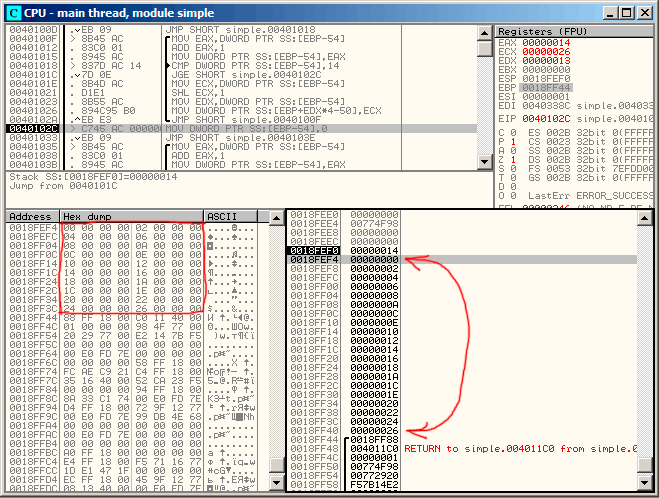
\includegraphics[scale=\FigScale]{patterns/13_arrays/1_simple/olly.png}
\caption{\olly: \RU{после заполнения массива}\EN{after array filling}}
\label{fig:array_simple_olly}
\end{figure}

\RU{А так как этот массив находится в стеке, то мы видим все его 20 элементов внутри стека.}
\EN{Since this array is located in stack, we see all its 20 elements inside of stack.}

\fi

\subsubsection{GCC}

\RU{То, что делает GCC 4.4.1:}\EN{Here is what GCC 4.4.1 does:}

\lstinputlisting[caption=GCC 4.4.1]{patterns/13_arrays/1_simple/simple_gcc.asm}

\RU{Кстати, переменная $a$ в нашем примере имеет тип \IT{int*} (то есть, указатель на \Tint{}) ~--- вы можете попробовать передать в другую функцию указатель на массив, но точнее было бы сказать, что передается указатель на первый элемент массива (а адреса остальных элементов массива можно вычислить очевидным образом).}\EN{By the way, $a$ variable has \IT{int*} type 
(the pointer to \Tint{})~---you can try to pass a pointer to array to another function, but it much correctly to say the pointer to the first array element is passed (addresses of another element's places are calculated in obvious way).}
\RU{Если индексировать этот указатель как \IT{a[idx]}, \IT{idx} просто прибавляется к указателю и возвращается элемент, расположенный там, куда ссылается вычисленный указатель.}\EN{If to index this pointer as \IT{a[idx]}, \IT{idx} just to be added to the pointer and the element placed there (to which calculated pointer is pointing) returned.}

\RU{Вот любопытный пример: строка символов вроде \IT{``string''} это массив из символов, 
и она имеет тип \IT{const char[]}.}\EN{An interesting example: string of characters like 
\IT{``string''} is array of characters and it has \IT{const char[]} type.}
\RU{К этому указателю также можно применять индекc.}
\EN{Index can also be applied to this pointer.}
\RU{И поэтому можно написать даже так:  \TT{``string''[i]} ~--- это совершенно легальное выражение в \CCpp!}
\EN{And that is why it is possible to write like \TT{``string''[i]}~---this is correct \CCpp expression!}

\ifdefined\IncludeARM
\subsection{ARM}

\subsubsection{\NonOptimizingKeilVI (\ARMMode)}

\lstinputlisting{patterns/13_arrays/1_simple/simple_Keil_ARM_O0.asm.\LANG}

\RU{Тип \Tint требует 32 бита для хранения (или 4 байта),}
\EN{\Tint type requires 32 bits for storage (or 4 bytes),}
\RU{так что для хранения 20 переменных типа \Tint, нужно $80$ (\TT{0x50}) байт.}
\EN{so to store 20 \Tint variables $80$ (\TT{0x50}) bytes are needed.}
\RU{Поэтому инструкция}\EN{So that is why the} \TT{\q{SUB SP, SP, \#0x50}} 
\RU{в прологе функции выделяет в локальном стеке под массив именно столько места.}
\EN{instruction in the function's prologie allocates exactly this amount of space in the stack.}

\RU{И в первом и во втором цикле, итератор цикла $i$ будет постоянно находится в регистре \Reg{4}.}
\EN{In both the first and second loops, the loop iterator $i$ is placed in the \Reg{4} register.}

\index{ARM!Optional operators!LSL}
\RU{Число, которое нужно записать в массив, вычисляется так: $i*2$, и это эквивалентно 
сдвигу на 1 бит влево, так что инструкция \TT{\q{MOV R0, R4,LSL\#1}} делает это.}
\EN{The number that is to be written into the array is calculated as $i*2$, which is effectively equivalent 
to shifting it left by one bit, so \TT{\q{MOV R0, R4,LSL\#1}} instruction does this.}

\index{ARM!\Instructions!STR}
\TT{\q{STR R0, [SP,R4,LSL\#2]}} \RU{записывает содержимое \Reg{0} в массив}\EN{writes the contents of \Reg{0} into the array}.
\RU{Указатель на элемент массива вычисляется так: \ac{SP} указывает на начало массива, \Reg{4} это $i$.}
\EN{Here is how a pointer to array element is calculated: \ac{SP} points to the start of the array, \Reg{4} is $i$.}
\RU{Так что сдвигаем $i$ на 2 бита влево, что эквивалентно умножению на $4$ 
(ведь каждый элемент массива занимает 4 байта) и прибавляем это к адресу начала массива.}
\EN{So shifting $i$ left by 2 bits is effectively equivalent to multiplication by $4$
(since each array element has a size of 4 bytes) and then it's added to the address of the start of the array.}

\index{ARM!\Instructions!LDR}
\RU{Во втором цикле используется обратная инструкция \TT{\q{LDR R2, [SP,R4,LSL\#2]}},
она загружает из массива нужное значение, и указатель на него вычисляется точно так же.}
\EN{The second loop has an inverse \TT{\q{LDR R2, [SP,R4,LSL\#2]}}
instruction, it loads the value we need from the array, and the pointer to it is calculated likewise.}

\subsubsection{\OptimizingKeilVI (\ThumbMode)}

\lstinputlisting{patterns/13_arrays/1_simple/simple_Keil_thumb_O3.asm.\LANG}

\RU{Код для thumb очень похожий.}\EN{Thumb code is very similar.}
\index{ARM!\Instructions!LSLS}
\RU{В thumb имеются отдельные инструкции для битовых сдвигов (как \TT{LSLS}), 
вычисляющие и число для записи в массив и адрес каждого элемента массива.}
\EN{Thumb mode has special instructions for bit shifting (like \TT{LSLS}),
which calculates the value to be written into the array and the address of each element in the array as well.}

\RU{Компилятор почему-то выделил в локальном стеке немного больше места, 
однако последние 4 байта не используются.}
\EN{The compiler allocates slightly more space in the local stack, however, the last 4 bytes are not used.}

\subsubsection{\NonOptimizing GCC 4.9.1 (ARM64)}

\lstinputlisting[caption=\NonOptimizing GCC 4.9.1 (ARM64)]{patterns/13_arrays/1_simple/ARM64_GCC491_O0.s.\LANG}

\fi

\section{\RU{Переполнение буфера}\EN{Buffer overflow}}
\label{subsec:bufferoverflow}
\myindex{\BufferOverflow}

\EN{\subsection{Reading outside array bounds}

So, array indexing is just \IT{array\lbrack{}index\rbrack}.
If you study the generated code closely, you'll probably note the missing index bounds checking,
which could check \IT{if it is less than 20}.
What if the index is 20 or greater?
That's the one \CCpp feature it is often blamed for.

Here is a code that successfully compiles and works:

\lstinputlisting{patterns/13_arrays/2_BO/r.c}

Compilation results (MSVC 2008):

\lstinputlisting[caption=\NonOptimizing MSVC 2008]{patterns/13_arrays/2_BO/r_msvc.asm}

The code produced this result:

\begin{figure}[h]
\centering
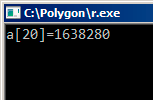
\includegraphics[scale=\NormalScale]{patterns/13_arrays/2_BO/olly_r3.png}
\caption{\olly: console output}
\label{fig:array_BO_olly_r3}
\end{figure}

It is just \IT{something} that was lying in the stack near to the array, 80 bytes away from its first element.

\clearpage
\myindex{\olly}
Let's try to find out where did this value come from, using \olly.

Let's load and find the value located right after the last array element:

\begin{figure}[H]
\centering
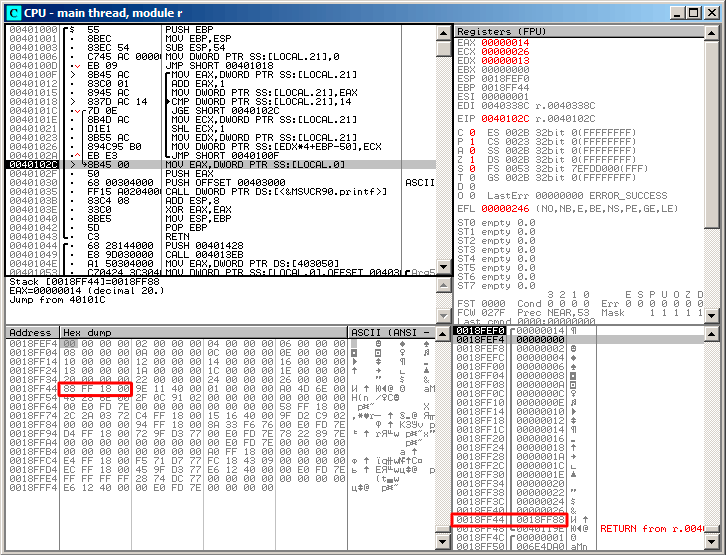
\includegraphics[scale=\FigScale]{patterns/13_arrays/2_BO/olly_r1.png}
\caption{\olly: reading of the 20th element and execution of \printf}
\label{fig:array_BO_olly_r1}
\end{figure}

What is this? 
Judging by the stack layout,
this is the saved value of the EBP register.
\clearpage
Let's trace further and see how it gets restored:

\begin{figure}[H]
\centering
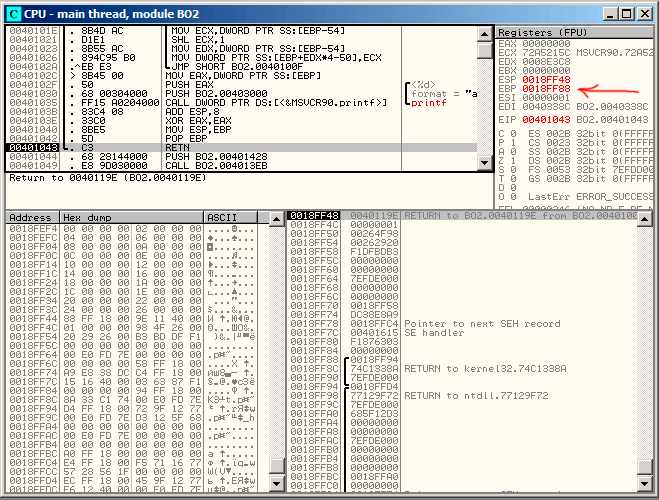
\includegraphics[scale=\FigScale]{patterns/13_arrays/2_BO/olly_r2.png}
\caption{\olly: restoring value of EBP}
\label{fig:array_BO_olly_r2}
\end{figure}

Indeed, how it could be different?
The compiler may generate some additional code to check the index value to be always
in the array's bounds (like in higher-level programming languages\footnote{Java, Python, etc})
but this makes the code slower.

}
\RU{\subsectionold{Чтение за пределами массива}

Итак, индексация массива --- это просто \IT{массив\lbrack{}индекс\rbrack}.  % TODO1 как-то плохо отображаются []
Если вы присмотритесь к коду, в цикле печати значений массива через \printf вы 
не увидите проверок индекса, \IT{меньше ли он двадцати?} 
А что будет если он будет 20 или больше? 
Эта одна из особенностей \CCpp, за которую их, собственно, и ругают.

Вот код, который и компилируется и работает:

\lstinputlisting{patterns/13_arrays/2_BO/r.c}

Вот результат компиляции в (MSVC 2008):

\lstinputlisting[caption=\NonOptimizing MSVC 2008]{patterns/13_arrays/2_BO/r_msvc.asm}

Данный код при запуске выдал вот такой результат:

\begin{figure}[h]
\centering
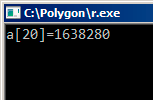
\includegraphics[scale=\NormalScale]{patterns/13_arrays/2_BO/olly_r3.png}
\caption{\olly: вывод в консоль}
\label{fig:array_BO_olly_r3}
\end{figure}

Это просто \IT{что-то}, что волею случая лежало в стеке рядом с массивом, 
через 80 байт от его первого элемента.

\clearpage
\myindex{\olly}
Попробуем узнать в \olly, что это за значение.
Загружаем и находим это значение, находящееся точно после последнего элемента массива:

\begin{figure}[H]
\centering
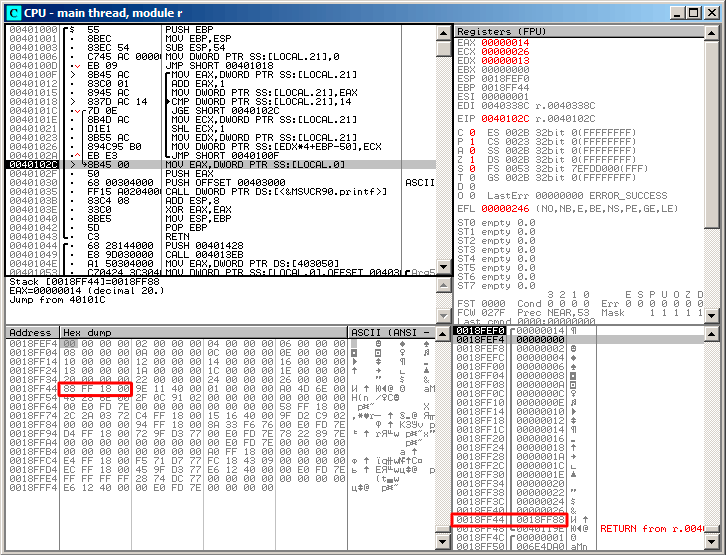
\includegraphics[scale=\FigScale]{patterns/13_arrays/2_BO/olly_r1.png}
\caption{\olly: чтение 20-го элемента и вызов \printf}
\label{fig:array_BO_olly_r1}
\end{figure}

Что это за значение? 
Судя по разметке стека, это сохраненное значение регистра EBP.
\clearpage
Трассируем далее, и видим, как оно восстанавливается:

\begin{figure}[H]
\centering
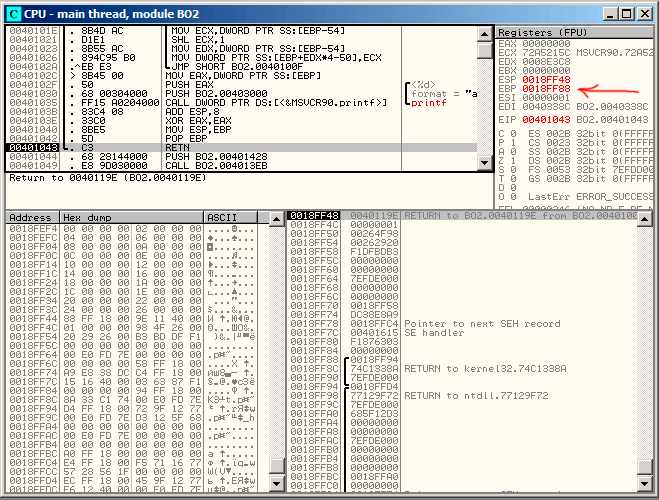
\includegraphics[scale=\FigScale]{patterns/13_arrays/2_BO/olly_r2.png}
\caption{\olly: восстановление EBP}
\label{fig:array_BO_olly_r2}
\end{figure}

Действительно, а как могло бы быть иначе? Компилятор мог бы встроить какой-то код, 
каждый раз проверяющий индекс на соответствие пределам массива, как в языках программирования 
более высокого уровня\footnote{Java, Python, итд.}, что делало бы запускаемый код медленнее.

}
\EN{\subsubsection{Writing beyond array bounds}

OK, we read some values from the stack \IT{illegally}, but what if we could write something to it?

Here is what we have got:

\lstinputlisting{patterns/13_arrays/2_BO/w.c}

\myparagraph{MSVC}

And what we get:

\lstinputlisting[caption=\NonOptimizing MSVC 2008]{patterns/13_arrays/2_BO/w_EN.asm}

The compiled program crashes after running. No wonder. Let's see where exactly does it is crash.

\clearpage
\myindex{\olly}

Let's load it into \olly, and trace until all 30 elements are written:

\begin{figure}[H]
\centering
\myincludegraphics{patterns/13_arrays/2_BO/olly_w1.png}
\caption{\olly: after restoring the value of EBP}
\label{fig:array_BO_olly_w1}
\end{figure}

\clearpage
Trace until the function end:

\begin{figure}[H]
\centering
\myincludegraphics{patterns/13_arrays/2_BO/olly_w2.png}
\caption{\olly: 
EIP was restored, but \olly can't disassemble at 0x15}
\label{fig:array_BO_olly_w2}
\end{figure}

Now please keep your eyes on the registers.

\EIP is 0x15 now. It is not a legal address for code---at least for win32 code!
We got there somehow against our will.
It is also interesting that the \EBP register contain 0x14,
\ECX and \EDX contain 0x1D.

Let's study stack layout a bit more.

After the control flow was passed to \TT{\main}, the value in the \EBP register was saved on the stack.
Then, 84 bytes were allocated for the array and the $i$ variable.
That's \TT{(20+1)*sizeof(int)}.
\ESP now points to the \TT{\_i} variable in the local stack and after the execution of 
the next \TT{PUSH something}, \IT{something} is appearing next to \TT{\_i}.

That's the stack layout while the control is in \main:

\begin{center}
\begin{tabular}{ | l | l | }
\hline
  \TT{ESP}    & 4 bytes allocated for $i$ variable \\
\hline
  \TT{ESP+4}  & 80 bytes allocated for \TT{a[20]} array \\
\hline
  \TT{ESP+84} & saved \EBP value \\
\hline
  \TT{ESP+88} & return address \\
\hline
\end{tabular}
\end{center}

\TT{a[19]=something} statement writes the last \Tint in the bounds of the array (in bounds so far!).

\TT{a[20]=something} statement writes \IT{something} to the place where the value of \EBP is saved.

Please take a look at the register state at the moment of the crash. In our case,
20 was written in the 20th element. 
At the function end, the function epilogue restores the original \EBP value.
(20 in decimal is \TT{0x14} in hexadecimal).
Then \RET gets executed, which is effectively equivalent to \TT{POP EIP} instruction.

The \RET instruction takes the return address from the stack (that is the address in \ac{CRT}),
which was called \main),
and 21 iss stored there (\TT{0x15} in hexadecimal).
The CPU traps at address \TT{0x15},
but there is no executable code there, so exception gets raised.

\myindex{\BufferOverflow}

Welcome! It is called a \IT{buffer overflow}\footnote{\href{http://go.yurichev.com/17132}{wikipedia}}.

Replace the \Tint array with a string (\Tchar array), create a long string deliberately
and pass it to the program, to the function, which doesn't check the length of the string and copies it in a short buffer,
and you'll able to point the program to an address to which it must jump.
It's not that simple in reality, but that is how it emerged.
Classic article about it: \AlephOne.

\myparagraph{GCC}

Let's try the same code in GCC 4.4.1. We get:

\lstinputlisting{patterns/13_arrays/2_BO/w_gcc.asm}

Running this in Linux will produce: \TT{Segmentation fault}.

\myindex{GDB}

If we run this in the GDB debugger, we get this:

\begin{lstlisting}
(gdb) r
Starting program: /home/dennis/RE/1 

Program received signal SIGSEGV, Segmentation fault.
0x00000016 in ?? ()
(gdb) info registers
eax            0x0	0
ecx            0xd2f96388	-755407992
edx            0x1d	29
ebx            0x26eff4	2551796
esp            0xbffff4b0	0xbffff4b0
ebp            0x15	0x15
esi            0x0	0
edi            0x0	0
eip            0x16	0x16
eflags         0x10202	[ IF RF ]
cs             0x73	115
ss             0x7b	123
ds             0x7b	123
es             0x7b	123
fs             0x0	0
gs             0x33	51
(gdb) 
\end{lstlisting}

The register values are slightly different than in win32 example, 
since the stack layout is slightly different too.

}
\RU{\subsectionold{Запись за пределы массива}

Итак, мы прочитали какое-то число из стека явно \IT{нелегально}, а что если мы запишем?

Вот что мы пишем:

\lstinputlisting{patterns/13_arrays/2_BO/w.c}

\subsubsectionold{MSVC}

И вот что имеем на ассемблере:

\lstinputlisting[caption=\NonOptimizing MSVC 2008]{patterns/13_arrays/2_BO/w_RU.asm}

Запускаете скомпилированную программу, и она падает. Немудрено. Но давайте теперь узнаем, где именно.

\clearpage
\myindex{\olly}

Загружаем в \olly, трассируем пока запишутся все 30 элементов:

\begin{figure}[H]
\centering
\myincludegraphics{patterns/13_arrays/2_BO/olly_w1.png}
\caption{\olly: после восстановления EBP}
\label{fig:array_BO_olly_w1}
\end{figure}

\clearpage
Доходим до конца функции:

\begin{figure}[H]
\centering
\myincludegraphics{patterns/13_arrays/2_BO/olly_w2.png}
\caption{\olly: EIP восстановлен, но \olly не может дизассемблировать по адресу 0x15}
\label{fig:array_BO_olly_w2}
\end{figure}

Итак, следите внимательно за регистрами.

\EIP теперь 0x15. Это явно нелегальный адрес для кода~--- по крайней мере, win32-кода! 
Мы там как-то очутились, причем, сами того не хотели. Интересен также тот факт, что в \EBP хранится 0x14, 
а в \ECX и \EDX хранится 0x1D.

Ещё немного изучим разметку стека.

После того как управление передалось в \main, в стек было сохранено значение \EBP. 
Затем для массива и переменной $i$ было выделено 84 байта. Это \TT{(20+1)*sizeof(int)}. 
\ESP сейчас указывает на переменную \TT{\_i} в локальном стеке и при исполнении следующего \INS{PUSH что-либо}, 
\IT{что-либо} появится рядом с \TT{\_i}.

Вот так выглядит разметка стека пока управление находится внутри \main:

\begin{center}
\begin{tabular}{ | l | l | }
\hline
  \TT{ESP}    & 4 байта выделенных для переменной $i$ \\
\hline
  \TT{ESP+4}  & 80 байт выделенных для массива \TT{a[20]} \\
\hline
  \TT{ESP+84} & сохраненное значение \EBP \\
\hline
  \TT{ESP+88} & адрес возврата \\
\hline
\end{tabular}
\end{center}

Выражение \TT{a[19]=что\_нибудь} записывает последний \Tint в пределах массива (пока что в пределах!).

Выражение \TT{a[20]=что\_нибудь} записывает \IT{что\_нибудь} на место где сохранено значение \EBP.

Обратите внимание на состояние регистров на момент падения процесса. В нашем случае 
в 20-й элемент записалось значение 20. 
И вот всё дело в том, что заканчиваясь, эпилог функции восстанавливал значение \EBP 
(20 в десятичной системе это как раз \TT{0x14} в шестнадцатеричной). 
Далее выполнилась инструкция \RET, которая на самом деле эквивалентна \TT{POP EIP}.

Инструкция \RET вытащила из стека адрес возврата (это адрес где-то внутри \ac{CRT}), которая вызвала \main),
а там было записано 21 в десятичной системе, то есть 0x15 в шестнадцатеричной. 
И вот процессор оказался по адресу 0x15, но исполняемого кода там нет, так что случилось исключение.

\myindex{\BufferOverflow}
Добро пожаловать! Это называется \IT{buffer overflow}\footnote{\href{http://go.yurichev.com/17132}{wikipedia}}.

Замените массив \Tint на строку (массив \Tchar), нарочно создайте слишком длинную строку, 
передайте её в ту программу, 
в ту функцию, которая не проверяя длину строки скопирует её в слишком короткий буфер, 
и вы сможете указать программе, по какому именно адресу перейти. 
Не всё так просто в реальности, конечно, но началось всё с этого.
Классическая статья об этом: \AlephOne.

\subsubsectionold{GCC}

Попробуем то же самое в GCC 4.4.1. У нас выходит такое:

\lstinputlisting{patterns/13_arrays/2_BO/w_gcc.asm}

Запуск этого в Linux выдаст: \TT{Segmentation fault}.

\myindex{GDB}
Если запустить полученное в отладчике GDB, получим:

\begin{lstlisting}
(gdb) r
Starting program: /home/dennis/RE/1 

Program received signal SIGSEGV, Segmentation fault.
0x00000016 in ?? ()
(gdb) info registers
eax            0x0	0
ecx            0xd2f96388	-755407992
edx            0x1d	29
ebx            0x26eff4	2551796
esp            0xbffff4b0	0xbffff4b0
ebp            0x15	0x15
esi            0x0	0
edi            0x0	0
eip            0x16	0x16
eflags         0x10202	[ IF RF ]
cs             0x73	115
ss             0x7b	123
ds             0x7b	123
es             0x7b	123
fs             0x0	0
gs             0x33	51
(gdb) 
\end{lstlisting}

Значения регистров немного другие, чем в примере win32, потому что разметка стека чуть другая.

}


\ifx\LITE\undefined
\section{\RU{Защита от переполнения буфера}\EN{Buffer overflow protection methods}}
\label{subsec:BO_protection}

\RU{В наше время пытаются бороться с этой напастью, не взирая на халатность программистов на \CCpp. 
В MSVC есть опции вроде}
\EN{There are several methods to protect against it, regardless of \CCpp programmers' negligence.
MSVC has options like}\footnote{
Wikipedia: \RU{описания защит, которые компилятор может вставлять в код}
\EN{compiler-side buffer overflow protection methods}:\\
\url{http://en.wikipedia.org/wiki/Buffer_overflow_protection}}:

\begin{lstlisting}
 /RTCs Stack Frame runtime checking
 /GZ Enable stack checks (/RTCs)
\end{lstlisting}

\index{x86!\Instructions!RET}
\index{Function prologue}
\index{Security cookie}
\RU{Один из методов, это в прологе функции вставлять в область локальных переменных 
некоторое случайное значение 
и в эпилоге функции, перед выходом, это число проверять. 
И если проверка не прошла, то не выполнять инструкцию \RET а остановиться (или зависнуть). 
Процесс зависнет, но это лучше, чем удаленная атака на ваш хост.}
\EN{One of the methods is to write random value among local variables to stack at function prologue 
and to check it in function epilogue before function exiting.
And if value is not the same, do not execute last instruction \RET, but halt (or hang).
Process will hang, but that is much better then remote attack to your host.}
    
\newcommand{\CANARYURL}
{
    \RU
    {
        \url{http://miningwiki.ru/wiki/\%D0\%9A\%D0\%B0\%D0\%BD\%D0\%B0\%D1\%80\%D0\%B5\%D0\%B9\%D0\%BA\%D0\%B0_\%D0\%B2_\%D1\%88\%D0\%B0\%D1\%85\%D1\%82\%D0\%B5}
    }
    \EN{
        \url{http://en.wikipedia.org/wiki/Domestic\_Canary\#Miner.27s\_canary}
    }
}

\index{Canary}
\RU{Это случайное значение иногда называют ``канарейкой''
\footnote{``canary'' в англоязычной литературе}, 
по аналогии с шахтной канарейкой\footnote{\CANARYURL},
их использовали шахтеры в свое время, чтобы определять, есть ли в шахте опасный газ.
}
\EN{This random value is called ``canary'' sometimes, it is related to miner's canary\footnote{\CANARYURL},
they were used by miners in these days, in order to detect poisonous gases quickly.}
\RU{Канарейки очень к нему чувствительны и либо проявляли сильное беспокойство, либо гибли от газа.}
\EN{Canaries are very sensetive to mine gases, they become very agitated in case of danger, or even dead.}

\RU{Если скомпилировать наш простейший пример работы с массивом}
\EN{If to compile our very simple array example}~(\ref{arrays_simple}) \InENRU \ac{MSVC} 
\RU{с опцией RTC1 или RTCs}\EN{with RTC1 and RTCs option}, \RU{в конце функции будет вызов 
функции}\EN{you will see call to} \TT{@\_RTC\_CheckStackVars@8}\RU{, проверяющей корректность ``канарейки''.}
\EN{ function at the function end, checking ``canary'' correctness.}

\RU{Посмотрим, как дела обстоят в GCC}\EN{Let's see how GCC handles this}. 
\RU{Возьмем пример из секции про}\EN{Let's take} \TT{alloca()}~(\ref{alloca})\EN{ example}:

\lstinputlisting{patterns/02_stack/04_alloca/2_1.c}

\RU{По умолчанию, без дополнительных ключей, GCC 4.7.3 вставит в код проверку ``канарейки''}
\EN{By default, without any additional options, GCC 4.7.3 will insert ``canary'' check into code}:

\lstinputlisting[caption=GCC 4.7.3]{patterns/13_arrays/3_BO_protection/gcc_canary.asm}

\RU{Случайное значение находится в}\EN{Random value is located in} \TT{gs:20}. 
\RU{Оно записывается в стек, затем, в конце функции, значение в стеке
сравнивается с корректной ``канарейкой'' в}\EN{It is to be written on the stack and then, at the function end,
value in the stack is compared with correct ``canary'' in} \TT{gs:20}. 
\RU{Если значения не равны, будет вызвана функция}\EN{If values are not equal to each other, } 
\TT{\_\_stack\_chk\_fail}\RU{ и в консоли мы увидим что-то вроде такого}\EN{ function will be called and we will see
something like that in console} (Ubuntu 13.04 x86):

\begin{lstlisting}
*** buffer overflow detected ***: ./2_1 terminated
======= Backtrace: =========
/lib/i386-linux-gnu/libc.so.6(__fortify_fail+0x63)[0xb7699bc3]
/lib/i386-linux-gnu/libc.so.6(+0x10593a)[0xb769893a]
/lib/i386-linux-gnu/libc.so.6(+0x105008)[0xb7698008]
/lib/i386-linux-gnu/libc.so.6(_IO_default_xsputn+0x8c)[0xb7606e5c]
/lib/i386-linux-gnu/libc.so.6(_IO_vfprintf+0x165)[0xb75d7a45]
/lib/i386-linux-gnu/libc.so.6(__vsprintf_chk+0xc9)[0xb76980d9]
/lib/i386-linux-gnu/libc.so.6(__sprintf_chk+0x2f)[0xb7697fef]
./2_1[0x8048404]
/lib/i386-linux-gnu/libc.so.6(__libc_start_main+0xf5)[0xb75ac935]
======= Memory map: ========
08048000-08049000 r-xp 00000000 08:01 2097586    /home/dennis/2_1
08049000-0804a000 r--p 00000000 08:01 2097586    /home/dennis/2_1
0804a000-0804b000 rw-p 00001000 08:01 2097586    /home/dennis/2_1
094d1000-094f2000 rw-p 00000000 00:00 0          [heap]
b7560000-b757b000 r-xp 00000000 08:01 1048602    /lib/i386-linux-gnu/libgcc_s.so.1
b757b000-b757c000 r--p 0001a000 08:01 1048602    /lib/i386-linux-gnu/libgcc_s.so.1
b757c000-b757d000 rw-p 0001b000 08:01 1048602    /lib/i386-linux-gnu/libgcc_s.so.1
b7592000-b7593000 rw-p 00000000 00:00 0
b7593000-b7740000 r-xp 00000000 08:01 1050781    /lib/i386-linux-gnu/libc-2.17.so
b7740000-b7742000 r--p 001ad000 08:01 1050781    /lib/i386-linux-gnu/libc-2.17.so
b7742000-b7743000 rw-p 001af000 08:01 1050781    /lib/i386-linux-gnu/libc-2.17.so
b7743000-b7746000 rw-p 00000000 00:00 0
b775a000-b775d000 rw-p 00000000 00:00 0
b775d000-b775e000 r-xp 00000000 00:00 0          [vdso]
b775e000-b777e000 r-xp 00000000 08:01 1050794    /lib/i386-linux-gnu/ld-2.17.so
b777e000-b777f000 r--p 0001f000 08:01 1050794    /lib/i386-linux-gnu/ld-2.17.so
b777f000-b7780000 rw-p 00020000 08:01 1050794    /lib/i386-linux-gnu/ld-2.17.so
bff35000-bff56000 rw-p 00000000 00:00 0          [stack]
Aborted (core dumped)
\end{lstlisting}

\index{MS-DOS}
gs\EMDASH\RU{это так называемый сегментный регистр, эти регистры широко использовались во времена MS-DOS 
и DOS-экстендеров.}\EN{is so-called segment register, these registers were used widely in MS-DOS and DOS-extenders
times.}
\RU{Сейчас их функция немного изменилась.}\EN{Today, its function is different.}
\index{TLS}
\index{Windows!TIB}
\RU{Если говорить коротко, в Linux \TT{gs} всегда указывает на \ac{TLS}~(\ref{TLS}) ~--- там находится различная 
информация, специфичная для выполняющегося треда}
\EN{If to say briefly, the \TT{gs} register in Linux is always pointing to the
\ac{TLS}~(\ref{TLS})~---various information specific to thread is stored there}
(\RU{кстати, в win32 эту же роль играет сегментный регистр \TT{fs},
он всегда указывает на}\EN{by the way, in win32 environment,
the \TT{fs} register plays the same role, it pointing to}
\ac{TIB} \footnote{\url{https://en.wikipedia.org/wiki/Win32_Thread_Information_Block}}). 

\RU{Больше информации можно почерпнуть из исходных кодов Linux (по крайней мере, в версии 3.11): 
в файле}\EN{More information can be found in Linux source codes (at least in 3.11 version), in}
\IT{arch/x86/include/asm/stackprotector.h}\RU{ в комментариях описывается эта переменная}
\EN{ file this variable is described in comments}.

\subsection{\OptimizingXcodeIV (\ThumbTwoMode)}

\RU{Возвращаясь к нашему простому примеру}\EN{Let's back to our simple array example}~(\ref{arrays_simple}),
\RU{можно посмотреть, как LLVM добавит проверку ``канарейки''}
\EN{again, now we can see how LLVM will check ``canary'' correctness}:

\lstinputlisting{patterns/13_arrays/3_BO_protection/simple_Xcode_thumb_O3.asm.\LANG}

\index{Unrolled loop}
\RU{Во-первых, как видно, LLVM ``развернул'' цикл и все значения записываются в массив по одному, 
уже вычисленные, 
потому что LLVM посчитал что так будет быстрее.}
\EN{First of all, as we see, LLVM made loop ``unrolled'' and all values are written into array one-by-one,
already calculated since LLVM concluded it will be faster.}
\RU{Кстати, инструкции режима ARM позволяют сделать это еще быстрее и это может быть вашим 
домашним заданием.}\EN{By the way, ARM mode instructions may help to do this even faster, 
and finding this way could be your homework.}

\RU{В конце функции мы видим сравнение ``канареек'' ~--- той что лежит в локальном стеке и корректной, 
на которую ссылается регистр \Reg{8}.}
\EN{At the function end wee see ``canaries'' comparison~---that laying in local stack and correct one,
to which the \Reg{8} register pointing.}
\index{ARM!\Instructions!IT}
\RU{Если они равны, срабатывает блок из четырех инструкций при помощи \TT{``ITTTT EQ''}, это запись
$0$ в \Reg{0}, эпилог функции и выход из нее.}
\EN{If they are equal to each other, 4-instruction block is triggered by \TT{``ITTTT EQ''}, it is
writing $0$ into \Reg{0}, function epilogue and exit.}
\RU{Если ``канарейки'' не равны, блок не срабатывает и происходит
переход на функцию}\EN{If ``canaries'' are not equal, block will not be executed,
and jump to} \TT{\_\_\_stack\_chk\_fail}\RU{, которая, вероятно, остановит работу программы.}
\EN{ function will be occurred, which, as I suppose, will halt execution.}
% TODO illustrate this!



\fi
\subsection{\RU{Еще немного о массивах}\EN{One more word about arrays}}

\RU{Теперь понятно, почему нельзя написать в исходном коде на \CCpp что-то вроде:}
\EN{Now we understand why it is impossible to write something like this in \CCpp code:}

\begin{lstlisting}
void f(int size)
{
    int a[size];
...
};
\end{lstlisting}

\RU{Чтобы выделить место под массив в локальном стеке, 
компилятору нужно знать размер массива, чего он на стадии компиляции, 
разумеется, знать не может.}
\EN{That's just because the compiler must know the exact array size to allocate space for 
it in the local stack layout on at the compiling stage.}

\myindex{\CLanguageElements!C99!variable length arrays}
\myindex{\CStandardLibrary!alloca()}
\RU{Если вам нужен массив произвольной длины, то выделите столько, сколько нужно, через \TT{malloc()}, 
а затем обращайтесь к выделенному блоку байт как к массиву того типа, который вам нужен.}
\EN{If you need an array of arbitrary size, allocate it by using \TT{malloc()}, then access the allocated memory block
as an array of variables of the type you need.}

\RU{Либо используйте возможность стандарта C99~ \InSqBrackets{\CNineNineStd 6.7.5/2},
и внутри это очень похоже на \IT{alloca()}~(\myref{alloca}).}
\EN{Or use the C99 standard feature \InSqBrackets{\CNineNineStd 6.7.5/2},
and it works like \IT{alloca()}~(\myref{alloca}) internally.}

\RU{Для работы в с памятью, можно также воспользоваться библиотекой сборщика мусора в Си.}
\EN{It's also possible to use garbage collecting libraries for C.}
\RU{А для языка Си++ есть библиотеки с поддержкой умных указателей.}
\EN{And there are also libraries supporting smart pointers for C++.}


\section{\RU{Массив указателей на строки}\EN{Array of pointers to strings}}
\label{array_of_pointers_to_strings}

\RU{Вот также пример массива указателей.}\EN{Here is also example of array of pointers.}

\lstinputlisting[caption=\RU{Получить имя месяца}\EN{Get month name},label=get_month1]{patterns/13_arrays/45_month_1D/month1.c.\LANG}

\subsection{x64}

\lstinputlisting[caption=\Optimizing MSVC 2013 x64]{patterns/13_arrays/45_month_1D/month1_MSVC_2013_x64_Ox.asm}

\RU{Код очень простой}\EN{The code is very simple}:

\begin{itemize}

\item
\index{x86!\Instructions!MOVSXD}
\RU{Первая инструкция MOVSXD копирует 32-битное значение из ECX (где передается аргумент $month$)
в RAX с знаковым расширением (потому что аргумент $month$ имеет тип \Tint).}
\EN{The first MOVSXD instruction copies 32-bit value from ECX (where $month$ argument is passed) 
to RAX with sign-extension (because $month$ argument has \Tint type).}
\RU{Причина расширения в том что это значение будет использоваться в вычислениях наряду с другими 64-битными
значениями.}
\EN{The reason of extension laying in the fact that this 32-bit value will be used in calculation among
with other 64-bit values.}
\RU{Таким образом, оно должно быть расширено до 64-битного}
\EN{Hence, it should be promoted to 64-bit value}
\footnote{\RU{Это немного странная вещь, но отрицательный индекс массива может быть передан как $month$ 
(отрицаительные индексы массивов будут рассмотрены позже: \ref{negative_array_indices}).
И если так будет, отрицательное значение типа \Tint будет расширено со знаком корректно
и соответствующий элемент перед таблицей будет выбран.
Всё это не будет корректно работать без знакового расширения.}
\EN{It is somewhat weird issue, but negative array index could be passed here as $month$
(negative array indices will be explained later: \ref{negative_array_indices}). 
And if it will, negative input \Tint value will be sign-extended correctly 
and the corresponding element before table will be picked. 
It will not work correctly without sign-extension.}}.

\item
\RU{Затем адрес таблицы указателей загружается в RCX.}
\EN{Then the address of the pointers table is loaded into RCX.}

\item
\RU{В конце концов, входное значение ($month$) умножается на 8 и прибавляется к адресу.}
\EN{Finally, the input value ($month$) is multiplied by 8 and added to the address.}
\RU{Действительно: мы в 64-битной среде и все адреса (или указатели) 
требуют для хранения именно 64 бита (или 8 байт).}
\EN{Indeed: we are in 64-bit environment and all address (or pointers) require exactly 64 bits (or 8 bytes) 
for storage.}
\RU{Следовательно, каждый элемент таблицы имеет ширину в 8 байт.}
\EN{Hence, each table element has width of 8 bytes.}
\RU{И вот почему для выбора элемента под нужным номером, нужно пропустить $month*8$ байт от начала.}
\EN{And that's why to pick element of specific number, $month*8$ bytes should be skipped from the start.}
\RU{Это то что делает MOV}\EN{That's what MOV does}.
\RU{В дополнении, эта инструкция также загружает элемент по этому адресу.}
\EN{In addition, this instruction also loads element at this address.}
\RU{Для 1, элемент будет указателем на строку содержащую ``February'', итд.}
\EN{For 1, an element would be pointer to the string containing ``February'' string, etc.}

\end{itemize}

\Optimizing GCC 4.9 \RU{может это сделать даже лучше}\EN{can do the job even better}
\footnote{\RU{В листинге осталось ``0+'', потому что вывод ассемблера GCC не так скурпулезен, чтобы убрать это}
\EN{``0+'' left in listing because GCC assembler output is not tidy enough for eliminating it}.
\RU{Это \IT{displacement} и он здесь нулевой.}\EN{It's \IT{displacement}, and it's zero here.}}:

\begin{lstlisting}[caption=\Optimizing GCC 4.9 x64]
	movsx	rdi, edi
	mov	rax, QWORD PTR month1[0+rdi*8]
	ret
\end{lstlisting}

\subsubsection{32-bit MSVC}

\RU{Скомпилируем также в 32-битном компиляторе MSVC:}\EN{Let's also compile it in 32-bit MSVC compiler:}

\lstinputlisting[caption=\Optimizing MSVC 2013 x86]{patterns/13_arrays/45_month_1D/month1_MSVC_2013_x86_Ox.asm}

\RU{Входное значение не нужно расширять до 64-битного значения, так что оно используется как есть.}
\EN{Input value not needed to be extended to 64-bit value, so it is used as is.}
\RU{И оно умножается на 4, потому что элементы таблицы имеют ширину 32 бита или 4 байта.}
\EN{And it's multiplied by 4, because table elements has width of 32-bit or 4 bytes.}

\ifdefined\IncludeARM
% FIXME move to another file
\subsection{32-\RU{битный}\EN{bit} ARM}

\subsubsection{ARM \RU{в режиме ARM}\EN{in ARM mode}}

\lstinputlisting[caption=\OptimizingKeilVI (\ARMMode)]{patterns/13_arrays/45_month_1D/month1_Keil_ARM_O3.s}

\RU{Адрес таблицы загружается в R1.}
\EN{Table address is loaded into R1.}
\index{ARM!\Instructions!LDR}
\RU{Всё остальное делается используя только одну инструкцию LDR.}
\EN{All the rest is done using only one LDR instruction.}
\RU{Входное значение $month$ сдвигается влево на 2 (что то же самое что и умножение на 4), это значение
прибавляется к R1 (где находится адрес таблицы) и затем элемент таблицы загружается по этому адресу.}
\EN{Then input $month$ value is shifted left by 2 (which is the same as multiplying by 4), this value added
to R1 (where address of table is) and then a table element is loaded at this address.}
\RU{32-битный элемент таблицы загружается в R0 из таблицы.}
\EN{32-bit table element is loaded into R0 from the table.}

\subsubsection{ARM \RU{в режиме Thumb}\EN{in Thumb mode}}

\RU{Код почти такой же, только менее плотный, потому что здесь, в инструкции LDR, нельзя задать суффикс LSL:}
\EN{The code is mostly the same, but less dense, because LSL suffix cannot be specified in LDR instruction here:}

\begin{lstlisting}
get_month1 PROC
        LSLS     r0,r0,#2
        LDR      r1,|L0.64|
        LDR      r0,[r1,r0]
        BX       lr
        ENDP
\end{lstlisting}

\subsection{ARM64}

\lstinputlisting[caption=\Optimizing GCC 4.9 ARM64]{patterns/13_arrays/45_month_1D/month1_GCC49_ARM64_O3.s}

\index{ARM!\Instructions!ADRP/ADD pair}
\RU{Адрес таблицы загружается в X1 используя пару ADRP/ADD.}
\EN{Table address is loaded into X1 using ADRP/ADD pair.}
\RU{Соответствующий элемент выбирается используя одну инструкцию LDR, которая берет W0
(регистр где находится значение входного аргумента $month$), сдвигает его на 3 бита влево
(что то же самое что и умножение на 8),
расширяет его учитывая знак (это то что означает суффикс ``sxtw'') и прибавляет к X0.}
\EN{Then corresponding element is picked using only one instruction LDR, which takes W0 
(register where input $month$ argument is), shifts it 3 bits left (which is the same as multiplying by 8), 
sign-extends it (this is what ``sxtw'' suffix mean) and adds to X0.}
\RU{Затем 64-битное значение загружается из таблицы в X0.}\EN{Then 64-bit value is loaded into X0 from the table.}
\fi

\ifdefined\IncludeMIPS
\subsection{MIPS}

\lstinputlisting[caption=\Optimizing GCC 4.4.5 (IDA)]{patterns/13_arrays/45_month_1D/MIPS_O3_IDA.lst.\LANG}
\fi

\subsection{\RU{Переполнение массива}\EN{Array overflow}}

\RU{Наша ф-ция принимает значения в пределах $0..11$, но что будет, если будет передано $12$?}
\EN{Our function accepts values in range of $0..11$, but what if $12$ will be passed?}
\RU{В таблице в этом месте нет элемента.}\EN{There are no element in table present at this place.}
\RU{Так что ф-ция загрузит какое-то значение, которое волею случая находится там, и вернет его.}
\EN{So, the function will load some value which happened to be located there, and return it.}
\RU{Позже, какая-то другая ф-ция попытается прочитать текстовую строку по этому адресу и, возможно, упадет.}
\EN{Soon after, some other function will try to get a text string at this address and may crash.}

\RU{Я скомпилировал этот пример в MSVC для win64 и открыл его в IDA чтобы посмотреть, что линкер расположил
после таблицы:}
\EN{I compiled the example in MSVC for win64 and opened it in IDA to see what linker placed after the table:}

\lstinputlisting[caption=\RU{Исполняемый файл в}\EN{Executable file in} IDA]{patterns/13_arrays/45_month_1D/MSVC2012_win64_1.lst}

\RU{Имена месяцев идут сразу после.}\EN{Month names are came right after.}
\RU{Наша программа все-таки крошечная, так что здесь не так уж много данных для расположения их в сегменте
данных, так что это имена месяцев.}
\EN{Our program is tiny after all, so there are no much data to pack in the data segment, 
so these are month names.}
\RU{Но я должен заметить, что там может быть действительно \IT{что угодно}, что линкер решит там расположить,
случайным образом.}
\EN{But I should to note that there might be really \IT{anything} what linker decided to put by chance.}

\RU{Так что будет если 12 будет передано в ф-цию?}\EN{So what if 12 will be passed to the function?}
\RU{Вернется 13-й элемент таблицы}\EN{13th table element will be returned}.
\RU{Посмотрим, как CPU будет обходиться с байтами там как с 64-битным значением:}
\EN{Let's see how CPU will treat the bytes there as 64-bit value:}

\lstinputlisting[caption=\RU{Исполняемый файл в}\EN{Executable file in} IDA]{patterns/13_arrays/45_month_1D/MSVC2012_win64_2.lst}

\RU{И это}\EN{And this is} 0x797261756E614A.
\RU{После этого, какая-от другая ф-ция (вероятно, работающая со строками) попытается загруждать байты
по этому адресу, ожидая найти там Си-строку.}
\EN{Soon after, some other function (presumably, string processing) will try to read bytes at 
this address expecting C-string there.}
\RU{И скорее всего упадет, потому что это значение не выглядит как действительный адрес.}
\EN{Most likely it will crash, because this value is don't look like a valid address.}

\subsubsection{\RU{Защита от переполнения массива}\EN{Array overflow protection}}
\epigraph{\RU{Если какая-нибудь неприятность может случиться, она случается}
\EN{If something can go wrong, it will}}{\RU{Закон Мерфи}\EN{Murphy's Law}}

\RU{Немного наивно ожидать что всякий программист, кто будет использовать вашу ф-цию или библиотеку,
никогда не передаст аргумент больше 11.}
\EN{It's a bit naïve to expect that every programmer who use your function or library will never pass
an argument larger than 11.}

\RU{Существует также хорошая философия ``fail early and fail loudly'' или ``fail-fast'',
которая учит сообщать об ошибках как можно раньше и останавливаться.}
\EN{There are also a good ``fail early and fail loudly'' or ``fail-fast'' philosophy, 
which teaches to report problems as early as possible and stop.}

\index{\CStandardLibrary!assert()}
\RU{Один из таких методов в \CCpp это макрос assert().}
\EN{One of such methods in \CCpp is assertions.}
\RU{Мы можем немного изменить нашу программу, чтобы она падала при передаче неверного значения:}
\EN{We can modify our program to fail if incorrect value is passed:}

\lstinputlisting[caption=assert() \RU{добавлен}\EN{added}]{patterns/13_arrays/45_month_1D/month1_assert.c}

\RU{Макрос будет проверять на верные значения во время каждого старта ф-ции и падать если не выражение.}
\EN{Assertion macro will check for valid values at each function start and fail if expression is false.}

\lstinputlisting[caption=\Optimizing MSVC 2013 x64]{patterns/13_arrays/45_month_1D/MSVC2013_x64_Ox_checked.asm}

\RU{На самом деле, assert() это не ф-ция, а макрос. Он проверяет условие и передает также номер строки и название
файла в другую ф-цию, которая покажет эту инфомарцию пользователю.}
\EN{In fact, assert() is not a function, but macro. It checks for condition, then pass also line number and file
name to another function which will show this information to user.}

\RU{Мы видим что здесь и имя файла и выражение закодировано в UTF-16.}
\EN{Here we see that both file name and condition was encoded in UTF-16.}
\RU{Номер строки также передается (это 29)}\EN{Line number is also passed (it's 29)}.

\RU{Этот механизм, пожалуй, одинаковый во всех компиляторах.}
\EN{This mechanism is same in probably all compilers.}
\RU{Вот что делает GCC}\EN{Here is what GCC does}:

\lstinputlisting[caption=\Optimizing GCC 4.9 x64]{patterns/13_arrays/45_month_1D/GCC491_x64_O3_checked.s}

\RU{Так что макрос в GCC также передает и имя ф-ции, для удобства.}
\EN{So the macro in GCC also pass function name for convenience.}

\RU{Ничего не бывает бесплатным: и проверки на корректность тоже.}
\EN{Nothing came for free: sanitizing check as well.}
\RU{Это может замедлить работу вашей программы, особенно если макрос assert() используется в маленькой
критичной ко времени ф-ции.}
\EN{It makes your program slower, especially if assert() macros used in small time-critical functions.}
\RU{Так что, например, MSVC оставляет проверки в Debug-билдах, но в Release-билдах они исчезают.}
\EN{So MSVC, for example, leaves checks in Debug builds, but in Release builds they all are disappear.}
 
\RU{Ядра Microsoft \gls{Windows NT} также идут в виде билдов ``checked'' и ``free''}
\EN{Microsoft \gls{Windows NT} kernels are also came in ``checked'' and ``free'' builds}
\footnote{\href{http://go.yurichev.com/17259}{MSDN}}.
\RU{Первые имеют проверки на валидность аргументов (отсюда ``checked''), вторые нет (отсюда ``free'',
т.е., ``свободые'' от проверок).}
\EN{First has validation checks (hence, ``checked''), second doesn't (hence, ``free'' of checks).}

% FIXME: ARM? MIPS?

\section{\RU{Многомерные массивы}\EN{Multidimensional arrays}}

\RU{Внутри, многомерный массив выглядит так же, как и линейный.}
\EN{Internally, a multidimensional array is essentially the same thing as a linear array.}

\RU{Ведь память компьютера линейная, это одномерный массив.
Но для удобства, этот одномерный массив легко представить как многомерный.}
\EN{Since the computer memory is linear, it is an one-dimensional array.
For convenience, this multi-dimensional array can be easily represented as one-dimensional.}

\RU{К примеру, вот как элементы массива $a[3][4]$ расположены в одномерном массиве из 12-и ячеек:}
\EN{For example, thit is how the elements of the $a[3][4]$ array are placed in one-dimensional array of 12 cells:}

\begin{table}[H]
\centering
\begin{tabular}{ | l | }
\hline
[0][0] \\
\hline
[0][1] \\
\hline
[0][2] \\
\hline
[0][3] \\
\hline
[1][0] \\
\hline
[1][1] \\
\hline
[1][2] \\
\hline
[1][3] \\
\hline
[2][0] \\
\hline
[2][1] \\
\hline
[2][2] \\
\hline
[2][3] \\
\hline
\end{tabular}
\caption{\RU{Двухмерный массив представляется в памяти как одномерный}
\EN{Two-dimensional array represented in memory as one-dimensional}}
\end{table}

\RU{Вот по каким адресам в памяти располагается каждая ячейка двухмерного массива 3*4:}
\EN{Here is how each cell of 3*4 array are placed in memory:}

\begin{table}[H]
\centering
\begin{tabular}{ | l | l | l | l | }
\hline                        
0 & 1 & 2 & 3 \\
\hline  
4 & 5 & 6 & 7 \\
\hline  
8 & 9 & 10 & 11 \\
\hline  
\end{tabular}
\caption{\RU{Адреса в памяти каждой ячейки двухмерного массива}
\EN{Memory addresses of each cell of two-dimensional array}}
\end{table}

\index{row-major order}
\RU{То есть, чтобы вычислить адрес нужного элемента, в начале умножаем первый индекс на 4 (ширину матрицы), 
затем прибавляем второй индекс.}
\EN{So, in order to calculate the address of the element we need, we first multiply the first index by
4 (matrix width) and then add the second index.}
\RU{Это называется}\EN{That's called} \IT{row-major order}, 
\RU{и такой способ представления массивов и матриц используется по крайней мере в}
\EN{and this method of array and matrix representation is used in at least} \CCpp \AndENRU Python. 
\EN{The term}\RU{Термин} \IT{row-major order} \RU{означает по-русски
примерно следующее: ``в начале записываем элементы первой строки, затем второй \dots и элементы последней 
строки в самом конце''.}
\EN{in plain English language means: ``first, write the elements of the first row, then the second row \dots 
and finally the elements of the last row''.}

\index{column-major order}
\index{FORTRAN}
\RU{Другой способ представления называется}\EN{Another method for representation is called} 
\IT{column-major order} 
(\RU{индексы массива используются в обратном порядке}\EN{the array indices are used in reverse order}) 
\RU{и это используется по крайней мере в}\EN{and it is used at least in} FORTRAN, MATLAB \AndENRU R. 
\RU{Термин }\IT{column-major order} \RU{означает по-русски
следующее: ``в начале записываем элементы первого столбца, затем второго \dots и элементы последнего столбца
в самом конце''.}
\EN{term in plain English language means: ``first, write the elements of the first column, then the second column \dots
and finally the elements of the last column''.}

\RU{Какой из способов лучше}\EN{Which method is better}?
\RU{Вообще, в терминах производительности и кэш-памяти, лучший метод организации данных это тот,
при котором к данным обращаются последовательно.}
\EN{In general, in terms of performance and cache memory, 
the best scheme for data organization is the one,
in which the elements are accessed sequentially.}
\RU{Так что если ваша ф-ция обращается к данным построчно, то \IT{row-major order} лучше,
и наоборот.}
\EN{So if your function accesses data per row, \IT{row-major order} is better, and vice versa.}

% subsections
\subsection{\RU{Пример с двумерным массивов}\EN{Two-dimensional array example}}

\EN{We will work with array of \Tchar type, meaning that each element require only one 
byte in memory.}
\RU{Мы будем работать с массивом типа \Tchar, это значит, что каждый элемент требует
только одного байта в памяти.}

\subsubsection{\RU{Пример с заполнением строки}\EN{Row filling example}}
\index{\olly}

\RU{Заполняем вторую строку значениями}\EN{Let's fill the second row with values:} $0 \ldots 3$:

\lstinputlisting[caption=\RU{Пример с заполнением строки}\EN{Row filling example}]{patterns/13_arrays/5_multidimensional/two1.c.\LANG}

\RU{Я обвел красным все три строки}\EN{I marked all three rows with red}. 
\RU{Видно что во второй теперь имеются байты}\EN{We see that second row now has values} 
0, 1, 2 \AndENRU 3:

\begin{figure}[H]
\centering
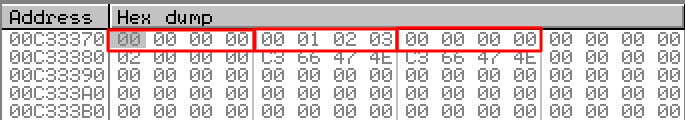
\includegraphics[scale=\NormalScale]{patterns/13_arrays/5_multidimensional/olly_2D_1.png}
\caption{\olly: \RU{массив заполнен}\EN{array is filled}}
\end{figure}

\subsubsection{\RU{Пример с заполнением столбца}\EN{Column filling example}}
\index{\olly}

\RU{Заполняем третий столбец значениями}\EN{Let's fill the third column with values:} $0 \ldots 2$.

\lstinputlisting[caption=\RU{Пример с заполнением столбца}\EN{Column filling example}]{patterns/13_arrays/5_multidimensional/two2.c.\LANG}

\RU{Здесь я также обвел красным три строки}\EN{I also marked three rows by red here}. 
\RU{Видно что в каждой строке, на третьей позиции, теперь записаны}
\EN{We see that in each row, at third position, these values are written:} 0, 1 \AndENRU 2.

\begin{figure}[H]
\centering
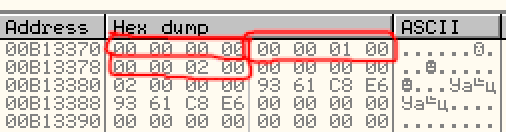
\includegraphics[scale=\NormalScale]{patterns/13_arrays/5_multidimensional/olly_2D_2.png}
\caption{\olly: \RU{массив заполнен}\EN{array is filled}}
\end{figure}

\subsection{\RU{Работа с двухмерным массивом как с одномерным}
\EN{Access two-dimensional array as one-dimensional}}

\RU{Мы можем легко убедиться, что можно работать с двухмерным массивом как с одномерным,
используя по крайней мере два метода:}
\EN{We can be easily assured that it's possible to access a two-dimensional array as one-dimensional array in at least two ways:}

\lstinputlisting{patterns/13_arrays/5_multidimensional/2D_as_1D.c.\LANG}

\RU{Компилируете и запускаете: мы увидим корректные значения.}
\EN{Compile and run it: it shows correct values.}

\RU{Очарователен результат работы MSVC 2013~--- все три процедуры одинаковые!}
\EN{What MSVC 2013 did is fascinating, all three routines are just the same!}

\lstinputlisting[caption=\Optimizing MSVC 2013 x64]{patterns/13_arrays/5_multidimensional/2D_as_1D_MSVC_2013_Ox_x64.asm.\LANG}

\RU{GCC сгенерировал практически одинаковые процедуры:}
\EN{GCC also generates equivalent routines, but slightly different:}

\lstinputlisting[caption=\Optimizing GCC 4.9 x64]{patterns/13_arrays/5_multidimensional/2D_as_1D_GCC49_x64_O3.s.\LANG}

\subsection{\RU{Пример с трехмерным массивом}\EN{Threedimensional array example}}

\RU{То же самое и для многомерных массивов.}\EN{Same thing about multidimensional arrays.}

\RU{На этот раз будем работать с массивом типа \Tint: каждый элемент требует 4 байта в памяти.}
\EN{Now we will work with array of \Tint type: each element require 4 bytes in memory.}

\RU{Попробуем}\EN{Let's see}:

\lstinputlisting[caption=\RU{простой пример}\EN{simple example}]{patterns/13_arrays/5_multidimensional/multi.c}

\subsubsection{x86}

\RU{В итоге}\EN{We got} (MSVC 2010):

\lstinputlisting[caption=MSVC 2010]{patterns/13_arrays/5_multidimensional/multi_msvc.asm}

\RU{В принципе, ничего удивительного. В \TT{insert()} для вычисления адреса нужного элемента массива, 
три входных аргумента перемножаются по формуле $address=600 \cdot 4 \cdot x + 30 \cdot 4 \cdot y + 4z$, 
чтобы представить массив трехмерным.
Не забывайте также, что тип \Tint 32-битный (4 байта), поэтому все коэффициенты нужно умножить на 4.}
\EN{Nothing special. For index calculation, three input arguments are multiplying 
by formula $address=600 \cdot 4 \cdot x + 30 \cdot 4 \cdot y + 4z$ to represent array as multidimensional.
Do not forget the \Tint type is 32-bit (4 bytes),
so all coefficients must be multiplied by 4.}

\lstinputlisting[caption=GCC 4.4.1]{patterns/13_arrays/5_multidimensional/multi_gcc.asm}

\RU{Компилятор GCC решил всё сделать немного иначе}\EN{GCC compiler does it differently}.
\RU{Для вычисления одной из операций ($30y$), GCC создал код, где нет самой операции умножения.}
\EN{For one of operations calculating ($30y$), GCC produced a code without multiplication instruction.}
\RU{Происходит это так}\EN{This is how it done}: 
$(y+y) \ll 4 - (y+y) = (2y) \ll 4 - 2y = 2 \cdot 16 \cdot y - 2y = 32y - 2y = 30y$. 
\RU{Таким образом, для вычисления $30y$ используется только операция сложения, 
операция битового сдвига и операция вычитания.}\EN{Thus, for $30y$ calculation, only one addition operation
used, one bitwise shift operation and one subtraction operation.}
\RU{Это работает быстрее}\EN{That works faster}.

\subsubsection{ARM + \NonOptimizingXcodeIV (\ThumbMode)}

\lstinputlisting[caption=\NonOptimizingXcodeIV (\ThumbMode)]{patterns/13_arrays/5_multidimensional/multi_Xcode_thumb_O0_\LANG.asm}

\NonOptimizing LLVM \RU{сохраняет все переменные в локальном стеке, хотя это и избыточно.}
\EN{saves all variables in local stack, however, it is redundant.}
\RU{Адрес элемента массива вычисляется по уже рассмотренной формуле.}
\EN{Address of array element is calculated by formula we already figured out.}

\subsubsection{ARM + \OptimizingXcodeIV (\ThumbMode)}

\lstinputlisting[caption=\OptimizingXcodeIV (\ThumbMode)]{patterns/13_arrays/5_multidimensional/multi_Xcode_thumb_O3_\LANG.asm}

\RU{Тут используются уже описанные трюки для замены умножения на операции сдвига, сложения и вычитания.}
\EN{Here is used tricks for replacing multiplication by shift, addition and subtraction we already considered.}

\index{ARM!\Instructions!RSB}
\index{ARM!\Instructions!SUB}
\RU{Также мы видим новую для себя инструкцию}\EN{Here we also see new instruction for us:} 
\TT{RSB} (\IT{Reverse Subtract}).
\RU{Она работает так же, как и \SUB, только меняет операнды местами.}
\EN{It works just as \SUB, but swapping operands with each other.}
\RU{Зачем?}\EN{Why?}
\index{ARM!Optional operators!LSL}
\SUB, \TT{RSB}, \RU{это те инструкции, ко второму операнду которых можно применить коэффициент сдвига, 
как мы видим и здесь}
\EN{are those instructions, to the second operand of which shift coefficient may be applied}: (\TT{LSL\#4}). 
\RU{Но этот коэффициент можно применить только ко второму операнду.}
\EN{But this coefficient may be applied only to second operand.}
\RU{Для коммутативных операций, таких как сложение или умножение, 
там операнды можно менять местами и это не влияет на результат.}
\EN{That's fine for commutative operations like addition or multiplication, operands may be swapped there
without result affecting.}
\RU{Но вычитание ~--- операция некоммутативная, так что, для этих случаев существует инструкция \TT{RSB}.}
\EN{But subtraction is non-commutative operation, so, for these cases, \TT{RSB} exist.}

\index{ARM!\Instructions!LDR.W}
\RU{Инструкция }\TT{``LDR.W R9, [R9]''} \RU{работает как}\EN{instruction works like} \LEA~(\ref{sec:LEA})
\RU{в x86, и здесь она ничего не делает, она избыточна.}\EN{in x86, but here it does nothing, it is redundant.}
\RU{Вероятно, компилятор несоптимизировал её.}\EN{Apparently, compiler not optimized it.}



\ifx\LITE\undefined
\subsection{\RU{Еще примеры}\EN{More examples}}

\RU{Компьютерный экран представляет собой двухмерный массив, но видеобуфер это линейный
одномерный массив}\EN{The computer screen is represented as a 2D array, but the video-buffer is 
a linear 1D array}. 
\RU{Мы рассматриваем это здесь}\EN{We talk about it here}: \myref{Mandelbrot_demo}.
\fi

\ifx\LITE\undefined
\section{\RU{Набор строк как двухмерный массив}\EN{Pack of strings as a two-dimensional array}}

\RU{Снова вернемся к примеру, который возвращает название месяца:}
\EN{Let's revisit the function that returns the name of a month:} \lstref{get_month1}.
\RU{Как видно, нужна как минимум одна операция загрузки из памяти для подготовки указателя на строку,
состоящую из имени месяца.}
\EN{As you see, at least one memory load operation is needed to prepare a pointer to the string
that's the month's name.}
\RU{Возможно ли избавиться от операции загрузки из памяти?}
\EN{Is it possible to get rid of this memory load operation?}
\RU{На самом деле, да, если представить список строк как двухмерный массив:}
\EN{In fact yes, if you represent the list of strings as a two-dimensional array:}

\lstinputlisting{patterns/13_arrays/55_month_2D/month2.c.\LANG}

\RU{Вот что получаем:}\EN{Here is what we've get:}

\lstinputlisting[caption=\Optimizing MSVC 2013 x64]{patterns/13_arrays/55_month_2D/MSVC2013_x64_Ox.asm.\LANG}

\RU{Здесь нет обращений к памяти вообще}\EN{There are no memory accesses at all}.
\RU{Всё что делает эта функция это вычисляет место, где находится первый символ названия месяца:}
\EN{All this function does is to calculate a point at which the first character of the name of the month is:} 
$pointer\_to\_the\_table + month * 10$.
\RU{Там также две инструкции LEA, которые работают как несколько инструкций MUL и MOV.}
\EN{There are also two LEA instructions, which effectively work as several MUL and MOV instructions.}

\RU{Ширина массива --- 10 байт}\EN{The width of the array is 10 bytes}. 
\RU{Действительно, самая длинная строка здесь это \q{September} (9 байт) плюс оконечивающий ноль --- это 10 байт.}
\EN{Indeed, the longest string here --- \q{September} --- is 9 bytes, and plus the terminating zero is 10 bytes.}
\RU{Остальные названия месяцев дополнены нулевыми байтами, чтобы они занимали столько же места (10 байт).}
\EN{The rest of the month names are padded by zero bytes, so they all occupy the same space (10 bytes).}
\RU{Таким образом, наша функция и работает быстрее, потому что все строки начинаются с тех адресов, 
которые легко вычислить.}
\EN{Thus, our function works even faster, because all string start at an address which can be
calculated easily.}

\Optimizing GCC 4.9 \RU{может еще короче}\EN{can do it even shorter}:

\begin{lstlisting}[caption=\Optimizing GCC 4.9 x64]
	movsx	rdi, edi
	lea	rax, [rdi+rdi*4]
	lea	rax, month2[rax+rax]
	ret
\end{lstlisting}

\RU{LEA здесь также используется для умножения на 10.}
\EN{LEA is also used here for multiplication by 10.}

\RU{Неоптимизирующие компиляторы делают умножение по-разному.}
\EN{Non-optimizing compilers do multiplication differently.}

\lstinputlisting[caption=\NonOptimizing GCC 4.9 x64]{patterns/13_arrays/55_month_2D/x64_GCC49_O0.asm.\LANG}

\NonOptimizing MSVC \RU{просто использует инструкцию IMUL}\EN{just use IMUL instruction}:
\index{x86!\Instructions!IMUL}

\lstinputlisting[caption=\NonOptimizing MSVC 2013 x64]{patterns/13_arrays/55_month_2D/MSVC2013_x64.asm.\LANG}

\index{\CompilerAnomaly}
\label{MSVC2013_anomaly}
\dots \RU{но вот что странно: зачем добавлять умножение на ноль и добавлять ноль к конечному результату?}
\EN{but one thing is weird here: why add multiplication by zero and adding zero to the final result?}
\RU{Я не знаю, это выглядит как выверт кодегенератора компилятора, который не был покрыт тестами
компилятора (так или иначе, итоговый код работает корректно).}
\EN{I don't know, this looks like a compiler code generator quirk, which wasn't caught by the compiler's tests
(the resulting code works correctly, after all).}
\RU{Я сознательно добавляю сюда такие фрагменты кода, чтобы читатель понимал, что иногда не нужно
ломать себе голову над подобными артефактами компиляторов.}
\EN{I intentionally add such pieces of code so the reader would understand, 
that sometimes one shouldn't puzzle over such compiler artifacts.}

\ifdefined\IncludeARM
\subsection{32-bit ARM}

\Optimizing Keil \RU{для режима Thumb использует инструкцию умножения}
\EN{for Thumb mode uses the multiplication instruction} MULS:

\lstinputlisting[caption=\OptimizingKeilVI (\ThumbMode)]{patterns/13_arrays/55_month_2D/Keil_O3_thumb.asm.\LANG}

\Optimizing Keil \RU{для режима ARM использует операции сложения и сдвига}\EN{for ARM mode uses add and 
shift operations}:

\lstinputlisting[caption=\OptimizingKeilVI (\ARMMode)]{patterns/13_arrays/55_month_2D/Keil_O3_ARM.asm.\LANG}

\subsection{ARM64}

\lstinputlisting[caption=\Optimizing GCC 4.9 ARM64]{patterns/13_arrays/55_month_2D/GCC49_ARM64.asm.\LANG}

\index{ARM!\Instructions!SXTW}
\index{ARM!\Instructions!ADRP/ADD pair}
\RU{SXTW используется для знакового расширения и расширения входного 32-битного значения в 64-битное и сохранения
его в X0.}
\EN{SXTW is used for sign-extension and promoting input 32-bit value into a 64-bit one and storing it in X0.}
\RU{Пара ADRP/ADD используется для загрузки адреса таблицы.}
\EN{ADRP/ADD pair is used for loading the address of the table.}
\RU{У инструкции ADD также есть суффикс LSL, что помогает с умножением.}
\EN{The ADD instructions also has a LSL suffix, which helps with multiplications.}
\fi

\ifdefined\IncludeMIPS
\subsection{MIPS}
\lstinputlisting[caption=\Optimizing GCC 4.4.5 (IDA)]{patterns/13_arrays/55_month_2D/MIPS_O3_IDA.lst.\LANG}
\fi

\subsection{\Conclusion{}}

\RU{Это немного олд-скульная техника для хранения текстовых строк.}
\EN{This is a bit old-school technique to store text strings.}
\RU{Такого можно много найти в \oracle, например.}
\EN{You may find a lot of it in \oracle, for example.}
\RU{Но я не уверен, стоит ли оно того на современных компьютерах.}
\EN{But I don't really know if it's worth doing on modern computers.}
\RU{Так или иначе, это был хороший пример массивов, так что я добавил его в эту книгу.}
\EN{Nevertheless, it was a good example of arrays, so I added it to this book.}

\fi
\subsection{\Conclusion{}}

\RU{Массив это просто набор значений в памяти, расположенных рядом друг с другом.}
\EN{An array is a pack of values in memory located adjacently.}
\RU{Это справедливо для любых типов элементов, включая структуры.}
\EN{It's true for any element type, including structures.}
\RU{Доступ к определенному элементу массива это просто вычисление его адреса.}
\EN{Access to a specific array element is just a calculation of its address.}

\ifdefined\IncludeExercises
\section{\Exercises}

\subsection{\Exercise \#1}
% matrix addition
\label{exercise_array_1}

\WhatThisCodeDoes\

\lstinputlisting[caption=MSVC 2010 + \TT{/O1}]{patterns/13_arrays/exercises/1_msvc.asm}

(/O1: \RU{оптимизация по размеру кода}\EN{minimize space}).

\lstinputlisting[caption=Keil 5.03 (\ARMMode) + \Othree]{patterns/13_arrays/exercises/1_ARM.s}

\lstinputlisting[caption=Keil 5.03 (\ThumbMode) + \Othree]{patterns/13_arrays/exercises/1_thumb.s}

\Answer\: \ref{exercise_solutions_arrays_1}.

\subsection{\Exercise \#2}
% matrix multiplication
\label{exercise_array_2}

\WhatThisCodeDoes\

\lstinputlisting[caption=MSVC 2010 + \TT{/O1}]{patterns/13_arrays/exercises/2_msvc.asm}

(/O1: \RU{оптимизация по размеру кода}\EN{minimize space}).

\lstinputlisting[caption=Keil 5.03 (\ARMMode) + \Othree]{patterns/13_arrays/exercises/2_ARM.s}

\lstinputlisting[caption=Keil 5.03 (\ThumbMode) + \Othree]{patterns/13_arrays/exercises/2_thumb.s}

\Answer\: \ref{exercise_solutions_arrays_2}.

\subsection{\Exercise \#3}
\label{exercise_array_3}

\WhatThisCodeDoes\

\EN{Try to determine array size, at least partially.}
\RU{Попробуйте определить размеры массива, хотя бы частично.}

\begin{lstlisting}[caption=MSVC 2010 /Ox]
_array$ = 8
_x$ = 12
_y$ = 16
_f	PROC
	mov	eax, DWORD PTR _x$[esp-4]
	mov	edx, DWORD PTR _y$[esp-4]
	mov	ecx, eax
	shl	ecx, 4
	sub	ecx, eax
	lea	eax, DWORD PTR [edx+ecx*8]
	mov	ecx, DWORD PTR _array$[esp-4]
	fld	QWORD PTR [ecx+eax*8]
	ret	0
_f	ENDP
\end{lstlisting}

\begin{lstlisting}[caption=Keil 5.03 (\ARMMode)]
f PROC
        RSB      r1,r1,r1,LSL #4
        ADD      r0,r0,r1,LSL #6
        ADD      r1,r0,r2,LSL #3
        LDM      r1,{r0,r1}
        BX       lr
        ENDP
\end{lstlisting}

\begin{lstlisting}[caption=Keil 5.03 (\ThumbMode)]
f PROC
        MOVS     r3,#0xf
        LSLS     r3,r3,#6
        MULS     r1,r3,r1
        ADDS     r0,r1,r0
        LSLS     r1,r2,#3
        ADDS     r1,r0,r1
        LDM      r1,{r0,r1}
        BX       lr
        ENDP
\end{lstlisting}

\Answer\: \ref{exercise_solutions_arrays_3}

\subsection{\Exercise \#4}
\label{exercise_array_4}

\WhatThisCodeDoes\

\EN{Try to determine array size, at least partially.}
\RU{Попробуйте определить размеры массива, хотя бы частично.}

\begin{lstlisting}[caption=MSVC 2010 /Ox]
_array$ = 8	
_x$ = 12	
_y$ = 16	
_z$ = 20	
_f	PROC
	mov	eax, DWORD PTR _x$[esp-4]
	mov	edx, DWORD PTR _y$[esp-4]
	mov	ecx, eax
	shl	ecx, 4
	sub	ecx, eax
	lea	eax, DWORD PTR [edx+ecx*4]
	mov	ecx, DWORD PTR _array$[esp-4]
	lea	eax, DWORD PTR [eax+eax*4]
	shl	eax, 4
	add	eax, DWORD PTR _z$[esp-4]
	mov	eax, DWORD PTR [ecx+eax*4]
	ret	0
_f	ENDP
\end{lstlisting}

\begin{lstlisting}[caption=Keil 5.03 (\ARMMode)]
f PROC
        RSB      r1,r1,r1,LSL #4
        ADD      r1,r1,r1,LSL #2
        ADD      r0,r0,r1,LSL #8
        ADD      r1,r2,r2,LSL #2
        ADD      r0,r0,r1,LSL #6
        LDR      r0,[r0,r3,LSL #2]
        BX       lr
        ENDP
\end{lstlisting}

\begin{lstlisting}[caption=Keil 5.03 (\ThumbMode)]
f PROC
        PUSH     {r4,lr}
        MOVS     r4,#0x4b
        LSLS     r4,r4,#8
        MULS     r1,r4,r1
        ADDS     r0,r1,r0
        MOVS     r1,#0xff
        ADDS     r1,r1,#0x41
        MULS     r2,r1,r2
        ADDS     r0,r0,r2
        LSLS     r1,r3,#2
        LDR      r0,[r0,r1]
        POP      {r4,pc}
        ENDP
\end{lstlisting}

\Answer\: \ref{exercise_solutions_arrays_4}

\subsection{\Exercise \#5}
\label{exercise_array_5}

\WhatThisCodeDoes\

\begin{lstlisting}[caption=MSVC 2012 /Ox /GS-]
COMM	_tbl:DWORD:064H

tv759 = -4	; size = 4
_main	PROC
	push	ecx
	push	ebx
	push	ebp
	push	esi
	xor	edx, edx
	push	edi
	xor	esi, esi
	xor	edi, edi
	xor	ebx, ebx
	xor	ebp, ebp
	mov	DWORD PTR tv759[esp+20], edx
	mov	eax, OFFSET _tbl+4
	npad	8
$LL6@main:
	lea	ecx, DWORD PTR [edx+edx]
	mov	DWORD PTR [eax+4], ecx
	mov	ecx, DWORD PTR tv759[esp+20]
	add	DWORD PTR tv759[esp+20], 3
	mov	DWORD PTR [eax+8], ecx
	lea	ecx, DWORD PTR [edx*4]
	mov	DWORD PTR [eax+12], ecx
	lea	ecx, DWORD PTR [edx*8]
	mov	DWORD PTR [eax], edx
	mov	DWORD PTR [eax+16], ebp
	mov	DWORD PTR [eax+20], ebx
	mov	DWORD PTR [eax+24], edi
	mov	DWORD PTR [eax+32], esi
	mov	DWORD PTR [eax-4], 0
	mov	DWORD PTR [eax+28], ecx
	add	eax, 40
	inc	edx
	add	ebp, 5
	add	ebx, 6
	add	edi, 7
	add	esi, 9
	cmp	eax, OFFSET _tbl+404
	jl	SHORT $LL6@main
	pop	edi
	pop	esi
	pop	ebp
	xor	eax, eax
	pop	ebx
	pop	ecx
	ret	0
_main	ENDP
\end{lstlisting}

\begin{lstlisting}[caption=Keil 5.03 (\ARMMode)]
main PROC
        LDR      r12,|L0.60|
        MOV      r1,#0
|L0.8|
        ADD      r2,r1,r1,LSL #2
        MOV      r0,#0
        ADD      r2,r12,r2,LSL #3
|L0.20|
        MUL      r3,r1,r0
        STR      r3,[r2,r0,LSL #2]
        ADD      r0,r0,#1
        CMP      r0,#0xa
        BLT      |L0.20|
        ADD      r1,r1,#1
        CMP      r1,#0xa
        MOVGE    r0,#0
        BLT      |L0.8|
        BX       lr
        ENDP

|L0.60|
        DCD      ||.bss||

        AREA ||.bss||, DATA, NOINIT, ALIGN=2

tbl
        %        400
\end{lstlisting}

\begin{lstlisting}[caption=Keil 5.03 (\ThumbMode)]
main PROC
        PUSH     {r4,r5,lr}
        LDR      r4,|L0.40|
        MOVS     r1,#0
|L0.6|
        MOVS     r2,#0x28
        MULS     r2,r1,r2
        MOVS     r0,#0
        ADDS     r3,r2,r4
|L0.14|
        MOVS     r2,r1
        MULS     r2,r0,r2
        LSLS     r5,r0,#2
        ADDS     r0,r0,#1
        CMP      r0,#0xa
        STR      r2,[r3,r5]
        BLT      |L0.14|
        ADDS     r1,r1,#1
        CMP      r1,#0xa
        BLT      |L0.6|
        MOVS     r0,#0
        POP      {r4,r5,pc}
        ENDP

        DCW      0x0000
|L0.40|
        DCD      ||.bss||

        AREA ||.bss||, DATA, NOINIT, ALIGN=2

tbl
        %        400
\end{lstlisting}

\Answer\: \ref{exercise_solutions_arrays_5}

\fi

\section{\IFRU{Битовые поля}{Bit fields}}
\label{sec:bitfields}

\IFRU{Немало функций задают различные флаги в аргументах при помощи битовых 
полей\footnote{bit fields в англоязычной литературе}.}
{A lot of functions defining input flags in arguments using bit fields.}
\index{\CLanguageElements!C99!bool}
\IFRU{Наверное, вместо этого, можно было бы использовать набор переменных типа \IT{bool}, но это было бы 
не очень экономно.}
{Of course, it could be substituted by \IT{bool}-typed variables set, but it is not frugally.}

\subsection{\IFRU{Проверка какого-либо бита}{Specific bit checking}}

\subsection{x86}

\RU{Например в Win32 API:}\EN{Win32 API example:}

\begin{lstlisting}
	HANDLE fh;

	fh=CreateFile ("file", GENERIC_WRITE | GENERIC_READ, FILE_SHARE_READ, NULL, OPEN_ALWAYS, FILE_ATTRIBUTE_NORMAL, NULL);
\end{lstlisting}

\RU{Получаем}\EN{We got} (MSVC 2010):

\begin{lstlisting}[caption=MSVC 2010]
	push	0
	push	128					; 00000080H
	push	4
	push	0
	push	1
	push	-1073741824				; c0000000H
	push	OFFSET $SG78813
	call	DWORD PTR __imp__CreateFileA@28
	mov	DWORD PTR _fh$[ebp], eax
\end{lstlisting}

\RU{Заглянем в файл}\EN{Let's take a look into} WinNT.h:

\begin{lstlisting}[caption=WinNT.h]
#define GENERIC_READ                     (0x80000000L)
#define GENERIC_WRITE                    (0x40000000L)
#define GENERIC_EXECUTE                  (0x20000000L)
#define GENERIC_ALL                      (0x10000000L)
\end{lstlisting}

\RU{Все ясно}\EN{Everything is clear}, 
\TT{GENERIC\_READ | GENERIC\_WRITE = 0x80000000 | 0x40000000 = 0xC0000000}, 
\RU{и это значение используется как второй аргумент для}
\EN{and that is value is used as the second argument for} \TT{CreateFile()}\footnote{\href{http://msdn.microsoft.com/en-us/library/aa363858(VS.85).aspx}{MSDN: CreateFile function}} function.

\RU{Как \TT{CreateFile()} будет проверять флаги?}\EN{How \TT{CreateFile()} will check flags?}

\index{Windows!KERNEL32.DLL}
\RU{Заглянем в KERNEL32.DLL от Windows XP SP3 x86 и найдем в функции \TT{CreateFileW()} в том числе и 
такой фрагмент кода:}
\EN{Let's take a look into KERNEL32.DLL in Windows XP SP3 x86 and we'll find
this fragment of code in the function \TT{CreateFileW}:}

\begin{lstlisting}[caption=KERNEL32.DLL (Windows XP SP3 x86)]
.text:7C83D429                 test    byte ptr [ebp+dwDesiredAccess+3], 40h
.text:7C83D42D                 mov     [ebp+var_8], 1
.text:7C83D434                 jz      short loc_7C83D417
.text:7C83D436                 jmp     loc_7C810817
\end{lstlisting}

\index{x86!\Instructions!TEST}
\RU{Здесь мы видим инструкцию \TEST, впрочем, она берет не весь второй аргумент функции, 
но только его самый старший байт (\TT{ebp+dwDesiredAccess+3}) и проверяет его на флаг 0x40 
(имеется ввиду флаг \TT{GENERIC\_WRITE}).}
\EN{Here we see \TEST instruction, it takes, however, not the whole second argument,
but only most significant byte (\TT{ebp+dwDesiredAccess+3}) and checks it for 0x40 flag
(meaning \TT{GENERIC\_WRITE} flag here)}

\index{x86!\Instructions!AND}
\RU{\TEST это то же что и \ANDIns, только без сохранения результата 
(вспомните что \CMP это то же что и \SUB, только без сохранения результатов}
\EN{\TEST is merely the same instruction as \ANDIns, but without result saving
(recall the fact \CMP instruction is merely the same as \SUB, but without result saving}~(\ref{CMPandSUB})).

\RU{Логика данного фрагмента кода примерно такая:}\EN{This fragment of code logic is as follows:}

\begin{lstlisting}
if ((dwDesiredAccess&0x40000000) == 0) goto loc_7C83D417
\end{lstlisting}

\index{x86!\Instructions!AND}
\index{x86!\Registers!ZF}
\RU{Если после операции \ANDIns останется этот бит, то флаг \ZF не будет поднят и условный переход 
\JZ не сработает. 
Переход возможен только если в переменной \TT{dwDesiredAccess} отсутствует бит \TT{0x40000000} ~--- 
тогда результат \ANDIns будет $0$, флаг \ZF будет поднят и переход сработает.}
\EN{If \ANDIns instruction leaving this bit, \ZF flag is to be cleared and \JZ conditional jump will not 
be triggered.
Conditional jump will be triggered only if \TT{0x40000000} bit is absent in the \TT{dwDesiredAccess} 
variable~---then \ANDIns result will be $0$, \ZF flag will be set and conditional jump is to be triggered.}

\RU{Попробуем GCC 4.4.1 и Linux:}\EN{Let's try GCC 4.4.1 and Linux:}

\begin{lstlisting}
#include <stdio.h>
#include <fcntl.h>

void main()
{
	int handle;

	handle=open ("file", O_RDWR | O_CREAT);
};
\end{lstlisting}

\RU{Получим}\EN{We got}:

\lstinputlisting[caption=GCC 4.4.1]{patterns/14_bitfields/check.asm}

\index{Linux!libc.so.6}
\index{syscalls}
\RU{Заглянем в реализацию функции \TT{open()} в библиотеке \TT{libc.so.6}, но обнаружим что там 
только вызов сисколла:}
\EN{Let's take a look into \TT{open()} function in the \TT{libc.so.6} library, but there is only syscall calling:}

\begin{lstlisting}[caption=open() (libc.so.6)]
.text:000BE69B                 mov     edx, [esp+4+mode] ; mode
.text:000BE69F                 mov     ecx, [esp+4+flags] ; flags
.text:000BE6A3                 mov     ebx, [esp+4+filename] ; filename
.text:000BE6A7                 mov     eax, 5
.text:000BE6AC                 int     80h             ; LINUX - sys_open
\end{lstlisting}

\RU{Значит, битовые поля флагов \TT{open()} вероятно проверяются где-то в ядре Linux.}
\EN{So, \TT{open()} bit fields apparently checked somewhere in Linux kernel.}

\RU{Разумеется, и стандартные библиотеки Linux и ядро Linux можно получить в виде исходников, 
но нам интересно попробовать разобраться без них.}
\EN{Of course, it is easily to download both Glibc and Linux kernel source code, 
but we are interesting to understand the matter without it.}

\RU{Итак, при вызове сисколла \TT{sys\_open}, управление в конечном итоге передается в \TT{do\_sys\_open} в ядре Linux 2.6. 
Оттуда ~--- в \TT{do\_filp\_open()} (эта функция находится в исходниках ядра в файле \TT{fs/namei.c}).}
\EN{So, as of Linux 2.6, when \TT{sys\_open} syscall is called, control eventually passed into \TT{do\_sys\_open} kernel function.
From there~---to the \TT{do\_filp\_open()} function (this function located in kernel source tree in the file \TT{fs/namei.c}).}

\newcommand{\URLREGPARM}{\url{http://ohse.de/uwe/articles/gcc-attributes.html\#func-regparm}}

\index{fastcall}
\label{regparm}
N.B. \RU{Помимо передачи параметров функции через стек, существует также возможность передавать 
некоторые из них через регистры. Это называется в том числе fastcall~(\ref{fastcall}).
Это работает немного быстрее, так как процессору не нужно обращаться к стеку, лежащему в памяти для чтения 
аргументов. 
В GCC есть опция \IT{regparm}\footnote{\URLREGPARM}, 
и с её помощью можно задать, сколько аргументов можно передать через регистры.}
\EN{Aside from common passing arguments via stack,
there is also a method of passing some of them
via registers. This is also called fastcall~(\ref{fastcall}).
This works faster since CPU not needed to access a stack in memory to read argument values.
GCC has option \IT{regparm}\footnote{\URLREGPARM},
and it is possible to set a number of arguments which might be passed via registers.}

\newcommand{\URLKERNELNEWB}{\url{http://kernelnewbies.org/Linux_2_6_20\#head-042c62f290834eb1fe0a1942bbf5bb9a4accbc8f}}
\newcommand{\CALLINGHFILE}{arch\textbackslash{}x86\textbackslash{}include\textbackslash{}asm\textbackslash{}calling.h}

\RU{Ядро Linux 2.6 собирается с опцией \TT{-mregparm=3}~\footnote{\URLKERNELNEWB}
\footnote{См. также файл \TT{\CALLINGHFILE} в исходниках ядра}.}
\EN{Linux 2.6 kernel compiled with \TT{-mregparm=3} option~\footnote{\URLKERNELNEWB}
\footnote{See also \TT{\CALLINGHFILE} file in kernel tree}.}

\RU{И для нас это означает, что первые три аргумента функции будут передаваться через регистры \EAX, 
\EDX и \ECX, 
а остальные через стек. Разумеется, если аргументов у функции меньше трех, то будет задействована 
только часть регистров.}
\EN{What it means to us, the first 3 arguments will be passed via \EAX, \EDX and \ECX registers, 
the rest ones via stack. Of course, if arguments number is less than 3, only part of registers
are to be used.}

\RU{Итак, качаем ядро 2.6.31, собираем его в Ubuntu: \TT{make vmlinux}, открываем в \IDA, 
находим функцию \TT{do\_filp\_open()}. В начале мы увидим подобное (комментарии мои):}
\EN{So, let's download Linux Kernel 2.6.31, compile it in Ubuntu: \TT{make vmlinux}, open it in \IDA, 
find the \TT{do\_filp\_open()} function. At the beginning, we will see (comments are mine):}

\lstinputlisting[caption=do\_filp\_open() (linux kernel 2.6.31)]{patterns/14_bitfields/check2_\LANG.asm}

\RU{GCC сохраняет значения первых трех аргументов в локальном стеке. Иначе, если эти три регистра 
не трогать вообще, то функции компилятора, распределяющей переменные по регистрам (так называемый 
\gls{register allocator}), 
будет очень тесно}
\EN{GCC saves first 3 arguments values in local stack. 
Otherwise, if compiler would not touch these registers, 
it would be too tight environment for compiler's \gls{register allocator}}.

\RU{Далее находим примерно такой фрагмент кода}\EN{Let's find this fragment of code}:

\lstinputlisting[caption=do\_filp\_open() (linux kernel 2.6.31)]{patterns/14_bitfields/check3.asm}

\RU{\TT{0x40} ~--- это то чему равен макрос \TT{O\_CREAT}. 
\TT{open\_flag} проверяется на наличие бита \TT{0x40} и если бит равен $1$, то выполняется следующие 
за \JNZ инструкции.}
\EN{\TT{0x40}~---is what \TT{O\_CREAT} macro equals to.
\TT{open\_flag} checked for \TT{0x40} bit presence, and if this bit is $1$, 
next \JNZ instruction is triggered.}



\subsubsection{ARM}

\IFRU{В ядре Linux 3.8.0 бит \TT{O\_CREAT} проверяется немного иначе.}
{\TT{O\_CREAT} bit is checked differently in Linux kernel 3.8.0.}

\begin{lstlisting}[caption=linux kernel 3.8.0]
struct file *do_filp_open(int dfd, struct filename *pathname,
		const struct open_flags *op)
{
...
	filp = path_openat(dfd, pathname, &nd, op, flags | LOOKUP_RCU);
...
}

static struct file *path_openat(int dfd, struct filename *pathname,
		struct nameidata *nd, const struct open_flags *op, int flags)
{
...
	error = do_last(nd, &path, file, op, &opened, pathname);
...
}


static int do_last(struct nameidata *nd, struct path *path,
		   struct file *file, const struct open_flags *op,
		   int *opened, struct filename *name)
{
...
	if (!(open_flag & O_CREAT)) {
    ...
		error = lookup_fast(nd, path, &inode);
    ...
	} else {
    ...
		error = complete_walk(nd);
        }
...
}
\end{lstlisting}

\IFRU{Вот как это выглядит в \IDA, ядро скомпилированное для режима ARM:}
{Here is how kernel compiled for ARM mode looks like in \IDA:}

\begin{lstlisting}[caption=do\_last() (vmlinux)]
...
.text:C0169EA8                 MOV             R9, R3  ; R3 - (4th argument) open_flag
...
.text:C0169ED4                 LDR             R6, [R9] ; R6 - open_flag
...
.text:C0169F68                 TST             R6, #0x40 ; jumptable C0169F00 default case
.text:C0169F6C                 BNE             loc_C016A128
.text:C0169F70                 LDR             R2, [R4,#0x10]
.text:C0169F74                 ADD             R12, R4, #8
.text:C0169F78                 LDR             R3, [R4,#0xC]
.text:C0169F7C                 MOV             R0, R4
.text:C0169F80                 STR             R12, [R11,#var_50]
.text:C0169F84                 LDRB            R3, [R2,R3]
.text:C0169F88                 MOV             R2, R8
.text:C0169F8C                 CMP             R3, #0
.text:C0169F90                 ORRNE           R1, R1, #3
.text:C0169F94                 STRNE           R1, [R4,#0x24]
.text:C0169F98                 ANDS            R3, R6, #0x200000
.text:C0169F9C                 MOV             R1, R12
.text:C0169FA0                 LDRNE           R3, [R4,#0x24]
.text:C0169FA4                 ANDNE           R3, R3, #1
.text:C0169FA8                 EORNE           R3, R3, #1
.text:C0169FAC                 STR             R3, [R11,#var_54]
.text:C0169FB0                 SUB             R3, R11, #-var_38
.text:C0169FB4                 BL              lookup_fast
...
.text:C016A128 loc_C016A128                            ; CODE XREF: do_last.isra.14+DC
.text:C016A128                 MOV             R0, R4
.text:C016A12C                 BL              complete_walk
...
\end{lstlisting}

\index{ARM!\Instructions!TST}
\index{x86!\Instructions!TEST}
\TT{TST} \IFRU{это аналог инструкции \TEST в x86.}{is analogical to a \TEST instruction in x86.}

\IFRU{Мы можем ``узнать'' визуально этот фрагмент кода по тому что в одном случае исполнится 
функция \TT{lookup\_fast()}, а в другом \TT{complete\_walk()}.}
{We can ``spot'' visually this code fragment by the fact the 
\TT{lookup\_fast()} will be executed
in one case and the \TT{complete\_walk()} in another case.}
\IFRU{Это соответствует исходному коду функции \TT{do\_last()}.}
{This is corresponding to the \TT{do\_last()} function source code.}

\RU{Макрос }\TT{O\_CREAT} \IFRU{здесь так же равен \TT{0x40}.}{macro is equals to \TT{0x40} here too.}




\section{\RU{Установка/сброс отдельного бита}\EN{Specific bit setting/clearing}}

\RU{Например}\EN{For example}:

\lstinputlisting{patterns/14_bitfields/set_reset.c}
\subsubsection{x86}

\IFRU{Имеем в итоге}{We got} (MSVC 2010):

\lstinputlisting[caption=MSVC 2010]{patterns/14_bitfields/set_reset_msvc.asm}

\index{x86!\Instructions!OR}
\IFRU{Инструкция \OR здесь добавляет в переменную еще один бит, игнорируя остальные.}
{\OR instruction adds one more bit to value while ignoring the rest ones.}

\index{x86!\Instructions!AND}
\IFRU{А \ANDIns сбрасывает некий бит. Можно также сказать, что \ANDIns здесь копирует все биты, кроме одного. 
Действительно, во втором операнде \ANDIns выставлены в единицу те биты, которые нужно сохранить, 
кроме одного, копировать который мы не хотим (и который $0$ в битовой маске).
Так проще понять и запомнить.}
{\ANDIns resetting one bit. It can be said, \ANDIns just copies all bits except one.
Indeed, in the second \ANDIns operand only those bits are set, which are needed to be saved,
except one bit we would not like to copy (which is $0$ in bitmask).
It is easier way to memorize the logic.}

\IFRU{Если скомпилировать в MSVC с оптимизацией (\Ox), то код будет еще короче:}
{If we compile it in MSVC with optimization turned on (\Ox), the code will be even shorter:}

\lstinputlisting[caption=\Optimizing MSVC]{patterns/14_bitfields/set_reset_msvc_Ox.asm}

\IFRU{Попробуем GCC 4.4.1 без оптимизации:}{Let's try GCC 4.4.1 without optimization:}

\lstinputlisting[caption=\NonOptimizing GCC]{patterns/14_bitfields/set_reset_gcc.asm}

\IFRU{Также избыточный код, хотя короче, чем у MSVC без оптимизации.}
{There is a redundant code present,
however, it is shorter then MSVC version without optimization.}

\IFRU{Попробуем теперь GCC с оптимизацией}{Now let's try GCC with optimization turned on} \Othree:

\lstinputlisting[caption=\Optimizing GCC]{patterns/14_bitfields/set_reset_gcc_O3.asm}

\IFRU{Уже короче. Важно отметить что через регистр \AH, компилятор работает с частью регистра \EAX, 
эта его часть от 8-го до 15-го бита включительно.}
{That's shorter.
It is worth noting the compiler works with the \EAX register part via the \AH 
register~---that is the \EAX register part from 8th to 15th bits inclusive.}

\RegTableOne{RAX}{EAX}{AX}{AH}{AL}

\index{x86!8086}
\index{x86!80386}
N.B. \IFRU{В 16-битном процессоре 8086 аккумулятор имел название \AX 
и состоял из двух 8-битных половин ~--- \AL (младшая часть) и \AH (старшая). 
В 80386 регистры были расширены до 32-бит, 
аккумулятор стал называться \EAX, но в целях совместимости, к его \IT{более старым} частям все еще можно 
обращаться как к \AX/\AH/\AL.}
{16-bit CPU 8086 accumulator was named \AX and consisted of two 8-bit 
halves~---\AL (lower byte) and \AH (higher byte).
In 80386 almost all registers were extended to 32-bit, accumulator was named \EAX, 
but for the sake of compatibility,
its \IT{older parts} may be still accessed as \AX/\AH/\AL registers.}

\IFRU{Из-за того, что все x86 процессоры ~--- наследники 16-битного 8086, эти \IT{старые} 16-битные опкоды короче 
нежели более новые 32-битные. 
Поэтому, инструкция \TT{``or ah, 40h''} занимает только 3 байта. 
Было бы логичнее сгенерировать здесь \TT{``or eax, 04000h''}, но это уже 5 байт, или даже 6 
(если регистр в первом операнде не \EAX).}
{Since all x86 CPUs are 16-bit 8086 CPU successors, these \IT{older} 16-bit opcodes are shorter 
than newer 32-bit opcodes.
That's why \TT{``or ah, 40h''} instruction occupying only 3 bytes.
It would be more logical way to emit here \TT{``or eax, 04000h''}
but that is 5 bytes, or even 6
(in case if register in first operand is not \EAX).}

\IFRU{Если мы скомпилируем этот же пример не только с включенной оптимизацией \Othree, 
но еще и с опцией \TT{regparm=3}, о которой я писал немного выше, то получится еще короче:}
{It would be even shorter if to turn on \Othree optimization flag and also set \TT{regparm=3}.}

\lstinputlisting[caption=\Optimizing GCC]{patterns/14_bitfields/set_reset_gcc_O3_regparm3.asm}

\index{Inline code}
\IFRU{Действительно ~--- первый аргумент уже загружен в \EAX, и прямо здесь можно начинать с ним работать. 
Интересно, что и пролог функции (\TT{``push ebp / mov ebp,esp''}) и эпилог (\TT{``pop ebp''}) 
функции можно смело выкинуть
за ненадобностью, 
но возможно GCC еще не так хорош для подобных оптимизаций по размеру кода. 
Впрочем, в реальной жизни, подобные короткие функции лучше всего автоматически делать в виде 
\IT{inline-функций} (\ref{inline_code}).}
{Indeed~---first argument is already loaded into \EAX, so it is possible to work with it in-place.
It is worth noting that both function prologue (\TT{``push ebp / mov ebp,esp''}) and epilogue (\TT{``pop ebp''})
can easily be omitted
here, but GCC probably is not good enough for such code size optimizations.
However, such short functions are better to be \IT{inlined functions} (\ref{inline_code}).}


\subsection{ARM + \OptimizingKeil + \ARMMode}

\begin{lstlisting}[caption=\OptimizingKeil + \ARMMode]
02 0C C0 E3          BIC     R0, R0, #0x200
01 09 80 E3          ORR     R0, R0, #0x4000
1E FF 2F E1          BX      LR
\end{lstlisting}

\index{ARM!\Instructions!BIC}
\index{ARM!\Instructions!ORR}
\TT{BIC} \RU{это ``логическое и'', аналог}\EN{is ``logical and'', analogical to} \ANDIns \InENRU x86.
\TT{ORR} \RU{это ``логическое или'', аналог}\EN{is ``logical or'', analogical to} \OR \InENRU x86.

\RU{Пока всё понятно}\EN{So far, so easy}.

\subsection{ARM + \OptimizingKeil + \ThumbMode}

\begin{lstlisting}[caption=\OptimizingKeil + \ThumbMode]
01 21 89 03          MOVS    R1, 0x4000
08 43                ORRS    R0, R1
49 11                ASRS    R1, R1, #5   ; generate 0x200 and place to R1
88 43                BICS    R0, R1
70 47                BX      LR
\end{lstlisting}

\RU{Вероятно, Keil решил, что код в режиме thumb}
\EN{Apparently, Keil concludes the code in thumb mode},
\RU{получающий}\EN{making} \TT{0x200} \RU{из}\EN{from} \TT{0x4000}, 
\RU{будет компактнее нежели код}\EN{will be more compact than code}, 
\RU{записывающий}\EN{writing} \TT{0x200} \RU{в какой-нибудь регистр}\EN{to arbitrary register}.

\index{ARM!\Instructions!ASRS}
\RU{Поэтому, при помощи инструкции}
\EN{So that is why, with the help of} \TT{ASRS} 
(\ASRdesc), \RU{это значение вычисляется как}\EN{this value is calculating as} $\TT{0x4000} \gg 5$.

\subsection{ARM + \OptimizingXcode + \ARMMode}
\label{anomaly:LLVM}
\index{\CompilerAnomaly}

\begin{lstlisting}[caption=\OptimizingXcode + \ARMMode]
42 0C C0 E3          BIC             R0, R0, #0x4200
01 09 80 E3          ORR             R0, R0, #0x4000
1E FF 2F E1          BX              LR
\end{lstlisting}

\RU{Код, который был сгенерирован LLVM, в исходном коде, на самом деле, выглядел бы так:}
\EN{The code was generated by LLVM, in source code form, in fact, could be looks like:}

\begin{lstlisting}
    REMOVE_BIT (rt, 0x4200);
    SET_BIT (rt, 0x4000);
\end{lstlisting}

\RU{И он делает то же самое что нам нужно}\EN{And it does exactly the same we need}. 
\RU{Но почему}\EN{But why} \TT{0x4200}? 
\RU{Возможно, это артефакт оптимизатора LLVM}
\EN{Perhaps, that is the LLVM optimizer's artifact}
\footnote{\RU{Это был}\EN{It was} LLVM build 2410.2.00 \RU{входящий в состав}\EN{bundled with} Apple Xcode 4.6.3}.
\RU{Возможно, ошибка оптимизатора компилятора, но создаваемый код все же работает верно.}
\EN{Probably, compiler's optimizer error, but generated code works correct anyway.}

\RU{Об аномалиях компиляторов, подробнее читайте здесь}
\EN{More about compiler's anomalies, read here}~(\ref{anomaly:Intel}).

\RU{Для режима Thumb}\EN{For thumb mode}, \OptimizingXcode \RU{генерирует точно такой же код}
\EN{generates likewise code}.




\section{\ShiftsSectionName}

\RU{Битовые сдвиги в \CCpp реализованы при помощи операторов $\ll$ и $\gg$.}
\EN{Bit shifts in \CCpp are implemented via $\ll$ and $\gg$ operators.}

\RU{Вот этот несложный пример иллюстрирует функцию, считающую количество бит-единиц во входной переменной:}
\EN{Here is a simple example of function, calculating number of $1$ bits in input variable:}

\lstinputlisting{patterns/14_bitfields/shifts.c}

\RU{В этом цикле, счетчик итераций \IT{i} считает от $0$ до $31$, а $1 \ll i$ будет от $1$ до \TT{0x80000000}. 
Описывая это словами, можно сказать 
\IT{сдвинуть единицу на $n$ бит влево}.
Т.е., в некотором смысле, выражение $1 \ll i$ последовательно выдаст все возможные позиции бит в 32-битном числе. 
Кстати, освободившийся бит справа всегда обнуляется. Макрос \TT{IS\_SET} проверяет наличие этого бита в \TT{a}.}
\EN{In this loop, iteration count value \IT{i} counting from $0$ to $31$, $1 \ll i$ statement will be counting 
from $1$ to \TT{0x80000000}.
Describing this operation in natural language, we would say \IT{shift $1$ by n bits left}.
In other words, $1 \ll i$ statement will consequently produce all possible bit positions in 32-bit number.
By the way, freed bit at right is always cleared. \TT{IS\_SET} macro is checking bit presence in the \TT{a}.}

\index{x86!\Instructions!SHL}
\begin{center}
	\begin{tikzpicture}[scale=0.7, every node/.style={scale=0.7}]
	\edef\bitsize{1cm}
	\tikzstyle{byte}=[draw,minimum size=\bitsize]	
	\tikzstyle{every path}=[thick]

	\node [draw,rectangle,minimum size=\bitsize] (a1) {7};
	\node [draw,rectangle,minimum size=\bitsize] (a2) [right of=a1] {6};
	\node [draw,rectangle,minimum size=\bitsize] (a3) [right of=a2] {5};
	\node [draw,rectangle,minimum size=\bitsize] (a4) [right of=a3] {4};
	\node [draw,rectangle,minimum size=\bitsize] (a5) [right of=a4] {3};
	\node [draw,rectangle,minimum size=\bitsize] (a6) [right of=a5] {2};
	\node [draw,rectangle,minimum size=\bitsize] (a7) [right of=a6] {1};
	\node [draw,rectangle,minimum size=\bitsize] (a8) [right of=a7] {0};

	\node (empty) [below of=a1] {};

	\node [draw,rectangle,minimum size=\bitsize] (b1) [below of=empty] {7};
	\node [draw,rectangle,minimum size=\bitsize] (b2) [right of=b1] {6};
	\node [draw,rectangle,minimum size=\bitsize] (b3) [right of=b2] {5};
	\node [draw,rectangle,minimum size=\bitsize] (b4) [right of=b3] {4};
	\node [draw,rectangle,minimum size=\bitsize] (b5) [right of=b4] {3};
	\node [draw,rectangle,minimum size=\bitsize] (b6) [right of=b5] {2};
	\node [draw,rectangle,minimum size=\bitsize] (b7) [right of=b6] {1};
	\node [draw,rectangle,minimum size=\bitsize] (b8) [right of=b7] {0};
	
	\node [shape=rectangle,draw,minimum size=\bitsize] (d) [left=of b1] {nowhere};
	\node [shape=rectangle,draw,minimum size=\bitsize] (c) [right=of b8] {0};
	
	\draw [->] (c.west) -- (b8.east);

	\draw [->] (a2.south) -- (b1.north);
	\draw [->] (a3.south) -- (b2.north);
	\draw [->] (a4.south) -- (b3.north);
	\draw [->] (a5.south) -- (b4.north);
	\draw [->] (a6.south) -- (b5.north);
	\draw [->] (a7.south) -- (b6.north);
	\draw [->] (a8.south) -- (b7.north);
	
	\draw [->] (a1.south) -- (d.north);

	\end{tikzpicture}
\end{center}


\index{x86!\Instructions!AND}
\RU{Макрос \TT{IS\_SET} на самом деле это операция логического И (\IT{AND}) 
и она возвращает $0$ если бита там нет, 
либо эту же битовую маску, если бит там есть. 
В \CCpp, конструкция \TT{if()} срабатывает, если выражение внутри её не ноль, пусть хоть $123456$, 
поэтому все будет работать.}
\EN{The \TT{IS\_SET} macro is in fact logical and operation (\IT{AND}) 
and it returns $0$ if specific bit is absent there,
or bit mask, if the bit is present.
\IT{if()} operator triggered in \CCpp if expression in it is not a zero, it might be even $123456$, that is why
it always working correctly.}

\subsection{x86}

\RU{Компилируем}\EN{Let's compile} (MSVC 2010):

\lstinputlisting[caption=MSVC 2010]{patterns/14_bitfields/shifts_MSVC_\LANG.asm}

\RU{Вот так работает SHL (\IT{SHift Left})}
\EN{That's how SHL (\IT{SHift Left}) working}.

\RU{Скомпилируем то же и в}\EN{Let's compile it in} GCC 4.4.1:

\lstinputlisting[caption=GCC 4.4.1]{patterns/14_bitfields/shifts_gcc.asm}

\RU{Инструкции сдвига также активно применяются при делении или умножении 
на числа-степени двойки ($1$, $2$, $4$, $8$, и т.д.).}
\EN{Shift instructions are often used in division and multiplications by power of two numbers 
($1$, $2$, $4$, $8$, etc).}

\RU{Например}\EN{For example}:

\begin{lstlisting}
unsigned int f(unsigned int a)
{
	return a/4;
};
\end{lstlisting}

\RU{Имеем в итоге}\EN{We got} (MSVC 2010):

\begin{lstlisting}[caption=MSVC 2010]
_a$ = 8							; size = 4
_f	PROC
	mov	eax, DWORD PTR _a$[esp-4]
	shr	eax, 2
	ret	0
_f	ENDP
\end{lstlisting}

\label{SHR}
\index{x86!\Instructions!SHR}
\RU{Инструкция \SHR (\IT{SHift Right}) в данном примере сдвигает число на 2 бита вправо. 
При этом, освободившиеся два бита слева (т.е., самые 
старшие разряды), выставляются в нули. А самые младшие 2 бита выкидываются. 
Фактически, эти два выкинутых бита ~--- остаток от деления.}
\EN{\SHR (\IT{SHift Right}) instruction in this example is shifting a number by 2 bits right.
Two freed bits at left (e.g., two most significant bits) are set to zero.
Two least significant bits are dropped.
In fact, these two dropped bits~---division operation remainder.}

\index{x86!\Instructions!SHR}
\RU{Инструкция \SHR работает так же, как и \SHL, только в другую сторону.}
\EN{\SHR instruction works just like as \SHL but in other direction.}

\input{shift_right}

\label{division_by_shifting}
\RU{Для того, чтобы это проще понять, представьте себе десятичную систему счисления и число $23$. 
$23$ можно разделить на $10$ просто откинув последний разряд ($3$ ~--- это остаток от деления). 
После этой операции останется $2$ как \glslink{quotient}{частное}.}
\EN{It can be easily understood if to imagine decimal numeral system and number $23$.
$23$ can be easily divided by $10$ just by dropping last digit ($3$~---is division remainder). 
$2$ is leaving after operation as a \gls{quotient}.}

\RU{Так и с умножением. Умножить на $4$ это просто сдвинуть число на 2 бита влево, 
вставив 2 нулевых бита справа (как два самых младших бита). 
Это как умножить $3$ на $100$ ~--- нужно просто дописать два нуля справа.}
\EN{The same story about multiplication.
Multiplication by $4$ is just shifting the number to the left by 2 bits,
while inserting 2 zero bits at right (as the last two bits).
It is just like to multiply $3$ by $100$~---we need just to add two zeroes at the right.}



\subsubsection{ARM + \OptimizingXcode + \ARMMode}

\begin{lstlisting}[caption=\OptimizingXcode + \ARMMode]
                MOV             R1, R0
                MOV             R0, #0
                MOV             R2, #1
                MOV             R3, R0
loc_2E54
                TST             R1, R2,LSL R3 ; set flags according to R1 & (R2<<R3)
                ADD             R3, R3, #1    ; R3++
                ADDNE           R0, R0, #1    ; if ZF flag is cleared by TST, R0++
                CMP             R3, #32
                BNE             loc_2E54
                BX              LR
\end{lstlisting}

\index{ARM!\Instructions!TST}
\TT{TST} \IFRU{это то же что и}{is the same things as} \TEST \InENRU x86.

\index{ARM!Optional operators!LSL}
\index{ARM!Optional operators!LSR}
\index{ARM!Optional operators!ASR}
\index{ARM!Optional operators!ROR}
\index{ARM!Optional operators!RRX}
\index{ARM!\Instructions!MOV}
\index{ARM!\Instructions!TST}
\index{ARM!\Instructions!CMP}
\index{ARM!\Instructions!ADD}
\index{ARM!\Instructions!SUB}
\index{ARM!\Instructions!RSB}
\IFRU{Как я уже указывал}{As I mentioned before}~(\ref{shifts_in_ARM_mode}),
\IFRU{в режиме ARM нет отдельной инструкции для сдвигов.}
{there are no separate shifting instructions in ARM mode.}
\IFRU{Однако, модификаторами}{However, there are modifiers} 
LSL (\IT{Logical Shift Left}), 
LSR (\IT{Logical Shift Right}), 
ASR (\IT{Arithmetic Shift Right}), 
ROR (\IT{Rotate Right}) \AndENRU 
RRX (\IT{Rotate Right with Extend}) \IFRU{можно дополнять некоторые инструкции, такие как}
{, which may be added to such instructions as} \MOV, \TT{TST},
\CMP, \ADD, \SUB, \TT{RSB}\footnote{\DataProcessingInstructionsFootNote}.

\IFRU{Эти модификаторы указывают, как сдвигать второй операнд, и на сколько.}
{These modificators are defines, how to shift second operand and by how many bits.}

\index{ARM!Optional operators!LSL}
\IFRU{Таким образом, инструкция }{Thus} \TT{``TST R1, R2,LSL R3''} 
\IFRU{здесь работает как}{instruction works here as} $R1 \land (R2 \ll R3)$.

\subsubsection{ARM + \OptimizingXcode + \ThumbTwoMode}

\index{ARM!\Instructions!LSL.W}
\index{ARM!\Instructions!LSL}
\IFRU{Почти такое же}{Almost the same}, 
\IFRU{только здесь применяется пара инструкций}{but here are two} 
\TT{LSL.W}/\TT{TST} 
\IFRU{вместо одной}{instructions are used instead of single} 
\TT{TST},
\IFRU{ведь в режиме thumb нельзя добавлять указывать модификатор}{because, in thumb mode, it is not
possible to define} \TT{LSL} \IFRU{прямо в}{modifier right in} \TT{TST}.

\begin{lstlisting}
                MOV             R1, R0
                MOVS            R0, #0
                MOV.W           R9, #1
                MOVS            R3, #0
loc_2F7A
                LSL.W           R2, R9, R3
                TST             R2, R1
                ADD.W           R3, R3, #1
                IT NE
                ADDNE           R0, #1
                CMP             R3, #32
                BNE             loc_2F7A
                BX              LR
\end{lstlisting}




\subsection{\IFRU{Пример вычисления CRC32}{CRC32 calculation example}}
\index{CRC32}

\newcommand{\URLCRCSRC}{\url{http://burtleburtle.net/bob/c/crc.c}}

\IFRU{Это распространенный табличный способ вычисления хеша алгоритмом 
CRC32\footnote{Исходник взят тут: \URLCRCSRC}.}
{This is very popular table-based CRC32 hash calculation 
technique\footnote{Source code was taken here: \URLCRCSRC}.}

\lstinputlisting{patterns/14_bitfields/CRC.c}

\index{\CLanguageElements!for}
\IFRU{Нас интересует функция \TT{crc()}. 
Кстати, обратите внимание на два инициализатора в выражении \TT{for()}: \TT{hash=len, i=0}. 
Стандарт \CCpp, конечно, допускает это. А в итоговом коде, вместо одной операции инициализации цикла, будет две.}
{We are interesting in the \TT{crc()} function only.
By the way, pay attention to two loop initializers in the \TT{for()} statement: \TT{hash=len, i=0}.
\CCpp standard allows this, of course.
Emitted code will contain two operations in loop initialization part
instead of usual one.}

\IFRU{Компилируем в MSVC с оптимизацией (\Ox). 
Для краткости, я приведу только функцию \TT{crc()}, с некоторыми комментариями.}
{Let's compile it in MSVC with optimization (\Ox).
For the sake of brevity, only \TT{crc()} function is listed here, with my comments.}

\lstinputlisting{patterns/14_bitfields/CRC_2_\IFRU{ru}{en}.asm}

\IFRU{Попробуем то же самое в GCC 4.4.1 с опцией \Othree:}
{Let's try the same in GCC 4.4.1 with \Othree option:}

\lstinputlisting{patterns/14_bitfields/CRC_gcc_O3_\IFRU{ru}{en}.asm}

\index{x86!\Instructions!NOP}
\index{x86!\Instructions!LEA}
\IFRU{GCC немного выровнял начало тела цикла по 8-байтной границе, для этого добавил 
\NOP и \TT{lea esi, [esi+0]} (что тоже \IT{холостая операция}). 
Подробнее об этом смотрите в разделе о npad~(\ref{sec:npad}).}
{GCC aligned loop start on a 8-byte border by adding \NOP and \TT{lea esi, [esi+0]}
(that is the \IT{idle operation} too).
Read more about it in npad section~(\ref{sec:npad}).}




\chapterold{\StructuresChapterName}

\RU{В принципе, структура в \CCpp это, с некоторыми допущениями, просто всегда лежащий рядом, 
и в той же последовательности, набор переменных, не обязательно одного типа
\footnote{\ac{AKA} \q{гетерогенный контейнер}}.}
\EN{A \CCpp structure, with some assumptions, is just a set of variables, always stored
in memory together, not necessary of the same type
\footnote{\ac{AKA} \q{heterogeneous container}}.}

% sections
\EN{\subsection{MSVC: SYSTEMTIME example}
\label{sec:SYSTEMTIME}

\newcommand{\FNSYSTEMTIME}{\footnote{\href{http://go.yurichev.com/17260}{MSDN: SYSTEMTIME structure}}}

Let's take the SYSTEMTIME\FNSYSTEMTIME{} win32 structure that describes time.

This is how it's defined:

\begin{lstlisting}[caption=WinBase.h]
typedef struct _SYSTEMTIME {
  WORD wYear;
  WORD wMonth;
  WORD wDayOfWeek;
  WORD wDay;
  WORD wHour;
  WORD wMinute;
  WORD wSecond;
  WORD wMilliseconds;
} SYSTEMTIME, *PSYSTEMTIME;
\end{lstlisting}

Let's write a C function to get the current time:

\lstinputlisting{patterns/15_structs/1_systemtime/systemtime.c}

We get (MSVC 2010):

\lstinputlisting[caption=MSVC 2010 /GS-]{patterns/15_structs/1_systemtime/systemtime.asm}

16 bytes are allocated for this structure in the local stack~---that is exactly \TT{sizeof(WORD)*8}
(there are 8 WORD variables in the structure).

\newcommand{\FNMSDNGST}{\footnote{\href{http://go.yurichev.com/17261}{MSDN: GetSystemTime function}}}

Pay attention to the fact that the structure begins with the \TT{wYear} field.
It can be said that a pointer to the SYSTEMTIME structure is passed to the \TT{GetSystemTime()}\FNSYSTEMTIME,
but it is also can be said that a pointer to the \TT{wYear} field is passed, and that is the same!
\TT{GetSystemTime()} writes the current year to the WORD pointer pointing to, then shifts 2 bytes
ahead, writes current month, etc., etc.

\clearpage
\subsection{\olly}
\myindex{\olly}

Let's compile this example in MSVC 2010 with \TT{/GS- /MD} keys and run it in \olly.

Let's open windows for data and stack at the address which is passed as the first argument of the
\TT{GetSystemTime()} function, and let's wait until it's executed. We see this:

\begin{figure}[H]
\centering
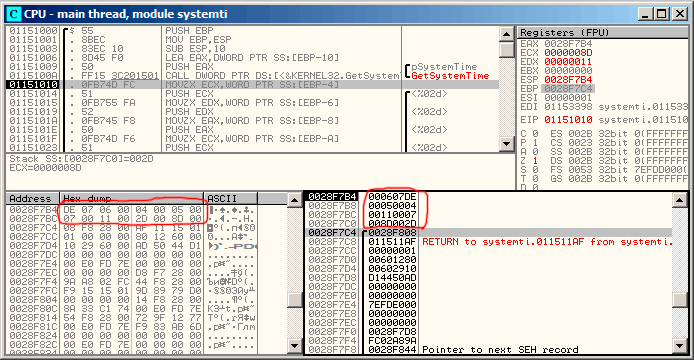
\includegraphics[scale=\FigScale]{patterns/15_structs/1_systemtime/olly_systemtime1.png}
\caption{\olly: \TT{GetSystemTime()} just executed}
\label{fig:struct_olly_1}
\end{figure}

The system time of the function execution on my computer is 9 december 2014, 22:29:52:

\begin{figure}[H]
\centering
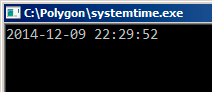
\includegraphics[scale=\NormalScale]{patterns/15_structs/1_systemtime/olly_systemtime2.png}
\caption{\olly: \printf output}
\label{fig:struct_olly_2}
\end{figure}

So we see these 16 bytes in the
data window: 
\begin{lstlisting}
DE 07 0C 00 02 00 09 00 16 00 1D 00 34 00 D4 03
\end{lstlisting}

Each two bytes represent one field of the structure. 
Since the \gls{endianness} is \IT{little endian}, 
we see the low byte first and then the high one.

Hence, these are the values currently stored in memory:

\begin{center}
\begin{tabular}{ | l | l | l | }
\hline
\headercolor{} Hexadecimal number & 
\headercolor{} decimal number & 
\headercolor{} field name \\
\hline
0x07DE & 2014	& wYear \\
\hline
0x000C & 12	& wMonth \\
\hline
0x0002 & 2	& wDayOfWeek \\
\hline
0x0009 & 9	& wDay \\
\hline
0x0016 & 22	& wHour \\
\hline
0x001D & 29	& wMinute \\
\hline
0x0034 & 52	& wSecond \\
\hline	
0x03D4 & 980	& wMilliseconds \\
\hline
\end{tabular}
\end{center}

The same values are seen in the stack window, but they are grouped as 32-bit values.

And then \printf just takes the values it needs and outputs them to the console.

Some values aren't output by \printf  (\TT{wDayOfWeek} and \TT{wMilliseconds}), 
but they are in memory right now, available for use.



\subsubsection{Replacing the structure with array}

The fact that the structure fields are just variables located side-by-side, can be easily demonstrated by doing the following.
Keeping in mind the \TT{SYSTEMTIME} structure description, it's possible to rewrite this simple example like this:

\lstinputlisting{patterns/15_structs/1_systemtime/systemtime2.c}

The compiler grumbles a bit:

\begin{lstlisting}
systemtime2.c(7) : warning C4133: 'function' : incompatible types - from 'WORD [8]' to 'LPSYSTEMTIME'
\end{lstlisting}

But nevertheless, it produces this code:

\lstinputlisting[caption=\NonOptimizing MSVC 2010]{patterns/15_structs/1_systemtime/systemtime2.asm}

And it works just as the same!

It is very interesting that the
result in assembly form cannot be distinguished from the result of the previous compilation.

So by looking at this code, one cannot say for sure if there was a structure declared, or an array. 

Nevertheless, no sane person would do it, as it is not convenient. 

Also the structure fields may be changed by developers, swapped, etc.

We will not study this example in \olly, because it will be just the same as in the case with the structure.

}
\RU{\section{MSVC: Пример SYSTEMTIME}
\label{sec:SYSTEMTIME}

\newcommand{\FNSYSTEMTIME}{\footnote{\href{http://go.yurichev.com/17260}{MSDN: SYSTEMTIME structure}}}

Возьмем, к примеру, структуру SYSTEMTIME\FNSYSTEMTIME{} из win32 описывающую время.

Она объявлена так:

\begin{lstlisting}[caption=WinBase.h]
typedef struct _SYSTEMTIME {
  WORD wYear;
  WORD wMonth;
  WORD wDayOfWeek;
  WORD wDay;
  WORD wHour;
  WORD wMinute;
  WORD wSecond;
  WORD wMilliseconds;
} SYSTEMTIME, *PSYSTEMTIME;
\end{lstlisting}

Пишем на Си функцию для получения текущего системного времени:

\lstinputlisting{patterns/15_structs/1_systemtime/systemtime.c}

Что в итоге (MSVC 2010):

\lstinputlisting[caption=MSVC 2010 /GS-]{patterns/15_structs/1_systemtime/systemtime.asm}

Под структуру в стеке выделено 16 байт ~--- именно столько будет \TT{sizeof(WORD)*8}
(в структуре 8 переменных с типом WORD).

\newcommand{\FNMSDNGST}{\footnote{\href{http://go.yurichev.com/17261}{MSDN: GetSystemTime function}}}

Обратите внимание на тот факт, что структура начинается с поля \TT{wYear}. 
Можно сказать, что в качестве аргумента для \TT{GetSystemTime()}\FNMSDNGST передается указатель на структуру 
SYSTEMTIME, но можно также сказать, что передается указатель на поле \TT{wYear}, 
что одно и тоже! 
\TT{GetSystemTime()} пишет текущий год в тот WORD на который указывает переданный указатель, 
затем сдвигается на 2 байта вправо, пишет текущий месяц, итд, итд.

\clearpage
\subsubsection{\olly}
\myindex{\olly}

Компилируем этот пример в MSVC 2010 с ключами \TT{/GS- /MD} и запускаем в \olly.
Открываем окна данных и стека по адресу, который передается в качестве первого аргумента в функцию \TT{GetSystemTime()}, 
ждем пока эта функция исполнится, и видим следующее:

\begin{figure}[H]
\centering
\myincludegraphics{patterns/15_structs/1_systemtime/olly_systemtime1.png}
\caption{\olly: \TT{GetSystemTime()} только что исполнилась}
\label{fig:struct_olly_1}
\end{figure}

Точное системное время на моем компьютере, в которое исполнилась функция, это 9 декабря 2014, 22:29:52:

\lstinputlisting[caption=Вывод \printf]{patterns/15_structs/1_systemtime/console.txt}

Таким образом, в окне данных мы видим следующие 16 байт: 
\begin{lstlisting}
DE 07 0C 00 02 00 09 00 16 00 1D 00 34 00 D4 03
\end{lstlisting}

Каждые два байта отражают одно поле структуры. 
А так как порядок байт (\gls{endianness}) \IT{little endian},
то в начале следует младший байт, затем старший.
Следовательно, вот какие 16-битные числа сейчас записаны в памяти:

\begin{center}
\begin{tabular}{ | l | l | l | }
\hline
\headercolor{} Шестнадцатеричное число & 
\headercolor{} десятичное число & 
\headercolor{} имя поля \\
\hline
0x07DE & 2014	& wYear \\
\hline
0x000C & 12	& wMonth \\
\hline
0x0002 & 2	& wDayOfWeek \\
\hline
0x0009 & 9	& wDay \\
\hline
0x0016 & 22	& wHour \\
\hline
0x001D & 29	& wMinute \\
\hline
0x0034 & 52	& wSecond \\
\hline	
0x03D4 & 980	& wMilliseconds \\
\hline
\end{tabular}
\end{center}

В окне стека, видны те же значения, только они сгруппированы как 32-битные значения.

Затем \printf просто берет нужные значения и выводит их на консоль.

Некоторые поля \printf не выводит (\TT{wDayOfWeek} и
\TT{wMilliseconds}), но они находятся в памяти и доступны для использования.



\subsection{Замена структуры массивом}

Тот факт, что поля структуры --- это просто переменные расположенные рядом, легко проиллюстрировать следующим образом.%

Глядя на описание структуры \TT{SYSTEMTIME}, можно переписать этот простой пример так:%

\lstinputlisting{patterns/15_structs/1_systemtime/systemtime2.c}

Компилятор немного ворчит:

\begin{lstlisting}
systemtime2.c(7) : warning C4133: 'function' : incompatible types - from 'WORD [8]' to 'LPSYSTEMTIME'
\end{lstlisting}

Тем не менее, выдает такой код:

\lstinputlisting[caption=\NonOptimizing MSVC 2010]{patterns/15_structs/1_systemtime/systemtime2.asm}

И это работает так же!

Любопытно что результат на ассемблере неотличим от предыдущего.
Таким образом, глядя на этот код, 
никогда нельзя сказать с уверенностью, была ли там объявлена структура, либо просто набор переменных.

Тем не менее, никто в здравом уме делать так не будет.

Потому что это неудобно. 
К тому же, иногда, поля в структуре могут меняться разработчиками, переставляться местами, итд.

С \olly этот пример изучать не будем, потому что он будет точно такой же, как и в случае со структурой.

}
\section{\RU{Выделяем место для структуры через malloc()}\EN{Let's allocate space for a structure using malloc()}}
\label{struct_malloc_example}

\RU{Однако, бывает и так, что проще хранить структуры не в стеке, а в \glslink{heap}{куче}:}
\EN{Sometimes it is simpler to place structures not the in local stack, but in the \gls{heap}:}

\lstinputlisting{patterns/15_structs/2_using_malloc/systemtime_malloc.c}

\RU{Скомпилируем на этот раз с оптимизацией (\Ox) чтобы было проще увидеть то, что нам нужно.}
\EN{Let's compile it now with optimization (\Ox) so it would be easy see what we need.}

\lstinputlisting[caption=\Optimizing MSVC]{patterns/15_structs/2_using_malloc/systemtime_malloc.asm}

\index{\CStandardLibrary!malloc()}
\RU{Итак, \TT{sizeof(SYSTEMTIME) = 16}, именно столько байт выделяется при помощи \TT{malloc()}. 
Она возвращает указатель на только что выделенный блок памяти в \EAX, который копируется в \ESI. 
Win32 функция \TT{GetSystemTime()} обязуется сохранить состояние \ESI, 
поэтому здесь оно нигде не сохраняется и продолжает использоваться после вызова \TT{GetSystemTime()}.}
\EN{So, \TT{sizeof(SYSTEMTIME) = 16} and that is exact number of bytes to be allocated by \TT{malloc()}.
It returns a pointer to a freshly allocated memory block in the \EAX register,
which is then moved into the \ESI register.
\TT{GetSystemTime()} win32 function takes care of saving value in \ESI,
and that is why it is not saved here and continues to be used after the \TT{GetSystemTime()} call.}

\index{x86!\Instructions!MOVZX}
\RU{
Новая инструкция ~--- \MOVZX (\IT{Move with Zero eXtend}). 
Она нужна почти там же где и \MOVSX, 
только всегда очищает остальные биты в 0. Дело в том, что \printf требует 32-битный тип \Tint, 
а в структуре лежит WORD ~--- это 16-битный беззнаковый тип. Поэтому копируя значение из WORD в \Tint, 
нужно очистить биты от 16 до 31, иначе там будет просто случайный мусор, оставшийся от предыдущих действий 
с регистрами.}
\EN{New instruction~---\MOVZX (\IT{Move with Zero eXtend}).
It may be used in most cases as \MOVSX, but it sets the remaining bits to 0.
That's because \printf requires a 32-bit \Tint, but we got a WORD in the structure~---that
is 16-bit unsigned type.
That's why by copying the value from a WORD into \Tint{}, bits from 16 to 31 must be cleared, 
because a random noise may be there, which is left from the previous operations on the register(s).}

\RU{В этом примере можно также представить структуру как массив 8-и WORD-ов:}
\EN{In this example, it's possible to represent the structure as an array of 8 WORDs:}

\lstinputlisting{patterns/15_structs/2_using_malloc/systemtime_malloc2.c}

\RU{Получим такое}\EN{We get}:

\lstinputlisting[caption=\Optimizing MSVC]{patterns/15_structs/2_using_malloc/systemtime_malloc2.asm}

\RU{И снова мы получаем идентичный код, неотличимый от предыдущего.}
\EN{Again, we got the code cannot be distinguished from the previous one.}
\RU{Но и снова нужно отметить, что в реальности так лучше не делать, 
если только вы не знаете точно, что вы делаете.}
\EN{And again it should be noted, you haven't to do this in practice, unless you really know what you are doing.}


\subsection{UNIX: struct tm}

% subsections here:
\EN{\subsection{Linux}

Let's take the \TT{tm} structure from \TT{time.h} in Linux for example:

\lstinputlisting{patterns/15_structs/3_tm_linux/GCC_tm.c}

Let's compile it in GCC 4.4.1:

\lstinputlisting[caption=GCC 4.4.1]{patterns/15_structs/3_tm_linux/GCC_tm_EN.asm}

Somehow, \IDA did not write the local variables' names in the local stack.
But since we already are experienced reverse engineers :-) we may do it without this information in 
this simple example.

\myindex{x86!\Instructions!LEA}

Please also pay attention to the \TT{lea edx, [eax+76Ch]}~---this instruction just adds \TT{0x76C} (1900) to value in \EAX,
but doesn't modify any flags. See also the relevant section about \LEA{}~(\myref{sec:LEA}).

\subsubsection{GDB}

Let's try to load the example into GDB
\footnote{The \IT{date} result is slightly corrected for demonstration purposes.
Of course, it's not possible to run GDB that quickly, in the same second.}:

\lstinputlisting[caption=GDB]{patterns/15_structs/3_tm_linux/GCC_tm_GDB.txt}

We can easily find our structure in the stack.
First, let's see how it's defined in \IT{time.h}:

\begin{lstlisting}[caption=time.h, label=struct_tm]
struct tm
{
  int	tm_sec;
  int	tm_min;
  int	tm_hour;
  int	tm_mday;
  int	tm_mon;
  int	tm_year;
  int	tm_wday;
  int	tm_yday;
  int	tm_isdst;
};
\end{lstlisting}

Pay attention that
32-bit \Tint is used here instead of WORD in SYSTEMTIME.
So, each field occupies 32-bit.

Here are the fields of our structure in the stack:

\begin{lstlisting}
0xbffff0dc:	0x080484c3	0x080485c0	0x000007de	0x00000000
0xbffff0ec:	0x08048301	0x538c93ed	0x00000025 sec	0x0000000a min
0xbffff0fc:	0x00000012 hour	0x00000002 mday	0x00000005 mon 	0x00000072 year
0xbffff10c:	0x00000001 wday	0x00000098 yday	0x00000001 isdst0x00002a30
0xbffff11c:	0x0804b090	0x08048530	0x00000000	0x00000000
\end{lstlisting}

Or as a table:

\begin{center}
\begin{tabular}{ | l | l | l | }
\hline
\headercolor{} Hexadecimal number & 
\headercolor{} decimal number & 
\headercolor{} field name \\
\hline
0x00000025 & 37 	& tm\_sec \\
\hline
0x0000000a & 10 	& tm\_min \\
\hline
0x00000012 & 18 	& tm\_hour \\	
\hline
0x00000002 & 2 		& tm\_mday \\	
\hline
0x00000005 & 5 		& tm\_mon \\	
\hline
0x00000072 & 114 	& tm\_year \\
\hline
0x00000001 & 1 		& tm\_wday \\	
\hline
0x00000098 & 152 	& tm\_yday \\	
\hline
0x00000001 & 1 		& tm\_isdst \\
\hline
\end{tabular}
\end{center}

Just like SYSTEMTIME (\myref{sec:SYSTEMTIME}), 

there are also other fields available that are not used, like tm\_wday, tm\_yday, tm\_isdst.
}
\RU{\subsectionold{Linux}

В Линуксе, для примера, возьмем структуру \TT{tm} из \TT{time.h}:

\lstinputlisting{patterns/15_structs/3_tm_linux/GCC_tm.c}

Компилируем при помощи GCC 4.4.1:

\lstinputlisting[caption=GCC 4.4.1]{patterns/15_structs/3_tm_linux/GCC_tm_RU.asm}

К сожалению, по какой-то причине, \IDA не сформировала названия локальных переменных в стеке. 
Но так как мы уже опытные реверсеры :-) то можем обойтись и без этого в таком простом примере.

\myindex{x86!\Instructions!LEA}
Обратите внимание на \TT{lea edx, [eax+76Ch]} ~--- эта инструкция прибавляет \TT{0x76C} (1900) к \EAX, 
но не модифицирует флаги. См. также соответствующий раздел об инструкции \LEA{}~(\myref{sec:LEA}).


\subsubsectionold{GDB}

Попробуем загрузить пример в GDB
\footnote{Результат работы \IT{date} немного подправлен в целях демонстрации.
Конечно же, в реальности, нельзя так быстро запустить GDB, чтобы значение секунд осталось бы таким же.}:

\lstinputlisting[caption=GDB]{patterns/15_structs/3_tm_linux/GCC_tm_GDB.txt}

Мы легко находим нашу структуру в стеке.
Для начала, посмотрим, как она объявлена в \IT{time.h}:

\begin{lstlisting}[caption=time.h, label=struct_tm]
struct tm
{
  int	tm_sec;
  int	tm_min;
  int	tm_hour;
  int	tm_mday;
  int	tm_mon;
  int	tm_year;
  int	tm_wday;
  int	tm_yday;
  int	tm_isdst;
};
\end{lstlisting}

Обратите внимание что здесь 32-битные \Tint вместо WORD в SYSTEMTIME.
Так что, каждое поле занимает 32-битное слово.

Вот поля нашей структуры в стеке:

\begin{lstlisting}
0xbffff0dc:	0x080484c3	0x080485c0	0x000007de	0x00000000
0xbffff0ec:	0x08048301	0x538c93ed	0x00000025 sec	0x0000000a min
0xbffff0fc:	0x00000012 hour	0x00000002 mday	0x00000005 mon 	0x00000072 year
0xbffff10c:	0x00000001 wday	0x00000098 yday	0x00000001 isdst0x00002a30
0xbffff11c:	0x0804b090	0x08048530	0x00000000	0x00000000
\end{lstlisting}

Либо же, в виде таблицы:

\begin{center}
\begin{tabular}{ | l | l | l | }
\hline
\headercolor{} Шестнадцатеричное число & 
\headercolor{} десятичное число & 
\headercolor{} имя поля \\
\hline
0x00000025 & 37 	& tm\_sec \\
\hline
0x0000000a & 10 	& tm\_min \\
\hline
0x00000012 & 18 	& tm\_hour \\	
\hline
0x00000002 & 2 		& tm\_mday \\	
\hline
0x00000005 & 5 		& tm\_mon \\	
\hline
0x00000072 & 114 	& tm\_year \\
\hline
0x00000001 & 1 		& tm\_wday \\	
\hline
0x00000098 & 152 	& tm\_yday \\	
\hline
0x00000001 & 1 		& tm\_isdst \\
\hline
\end{tabular}
\end{center}

Как и в примере с SYSTEMTIME (\myref{sec:SYSTEMTIME}), здесь есть и другие поля, готовые для использования, 
но в нашем примере они не используются, например, tm\_wday, tm\_yday, tm\_isdst.
}
\EN{\subsubsection{ARM}

\myparagraph{\OptimizingKeilVI (\ThumbMode)}

Same example:

\lstinputlisting[caption=\OptimizingKeilVI (\ThumbMode)]{patterns/15_structs/3_tm_linux/ARM/tm_ARM_keil_thumb.asm}

\myparagraph{\OptimizingXcodeIV (\ThumbTwoMode)}

\IDA \q{knows} the \TT{tm} structure 
(because \IDA \q{knows} the types of the arguments of library functions like \TT{localtime\_r()}), 

so it shows here structure elements accesses and their names.

\lstinputlisting[caption=\OptimizingXcodeIV (\ThumbTwoMode)]{patterns/15_structs/3_tm_linux/ARM/tm_ARM_xcode_thumb.asm}
}
\RU{\subsection{ARM}

\subsubsection{\OptimizingKeilVI (\ThumbMode)}

Этот же пример:

\lstinputlisting[caption=\OptimizingKeilVI (\ThumbMode)]{patterns/15_structs/3_tm_linux/ARM/tm_ARM_keil_thumb.asm}

\subsubsection{\OptimizingXcodeIV (\ThumbTwoMode)}

\IDA \q{узнала} структуру \TT{tm} 
(потому что \IDA \q{знает} типы аргументов библиотечных функций, 
таких как \TT{localtime\_r()}), 
поэтому показала здесь обращения к отдельным элементам структуры и присвоила им имена
.

\lstinputlisting[caption=\OptimizingXcodeIV (\ThumbTwoMode)]{patterns/15_structs/3_tm_linux/ARM/tm_ARM_xcode_thumb.asm}
}
\EN{\subsectionold{MIPS}

\lstinputlisting[caption=\Optimizing GCC 4.4.5 (IDA),numbers=left]{patterns/15_structs/3_tm_linux/MIPS/MIPS_O3_IDA_EN.lst}

This is an example where the branch delay slots can confuse us.

For example, there is the instruction \q{addiu \$a1, 1900} at line 35 which adds 1900 to the year number.

It's executed before the corresponding JALR at line 34, do not forget about it.

}
\RU{\subsection{MIPS}

\lstinputlisting[caption=\Optimizing GCC 4.4.5 (IDA),numbers=left]{patterns/15_structs/3_tm_linux/MIPS/MIPS_O3_IDA_RU.lst}

Это тот пример, где branch delay slot-ы могут нас запутать.

Например, в строке 35 есть инструкция \q{addiu \$a1, 1900}, добавляющая 1900 к числу года.

Но она исполняется перед исполнением соответствующей JALR в строке 34, не забыайте.

}
% subsection:
\EN{\subsubsection{Structure as a set of values}

In order to illustrate that the structure is just variables laying side-by-side in one place, 
let's rework our example while looking at the \IT{tm} structure definition again: \lstref{struct_tm}.

\lstinputlisting{patterns/15_structs/3_tm_linux/as_array/GCC_tm2.c}

\myindex{\CStandardLibrary!localtime\_r()}
N.B. 
The pointer to the \TT{tm\_sec} field is passed into \TT{localtime\_r}, i.e., 
to the first element of the \q{structure}.

The compiler warns us:

\begin{lstlisting}[caption=GCC 4.7.3]
GCC_tm2.c: In function 'main':
GCC_tm2.c:11:5: warning: passing argument 2 of 'localtime_r' from incompatible pointer type [enabled by default]
In file included from GCC_tm2.c:2:0:
/usr/include/time.h:59:12: note: expected 'struct tm *' but argument is of type 'int *'
\end{lstlisting}

But nevertheless, it generates this:

\lstinputlisting[caption=GCC 4.7.3]{patterns/15_structs/3_tm_linux/as_array/GCC_tm2.asm}

This code is identical to what we saw previously and it is
not possible to say, was it a structure in original source code or just a pack of variables.

And this works. 
However, it is not recommended to do this in practice. 

Usually, non-optimizing compilers allocates variables in the local stack in the 
same order as they were declared in the function.

Nevertheless, there is no guarantee.

By the way, some other compiler may warn about the \TT{tm\_year}, \TT{tm\_mon}, \TT{tm\_mday},
\TT{tm\_hour}, \TT{tm\_min} variables, but not \TT{tm\_sec}
 are used without being initialized.

Indeed, the compiler is not aware that these are to be filled by\\
\TT{localtime\_r()} function.

We chose this example, since all structure fields are of type \Tint.%

This would not work if structure fields are 16-bit (\TT{WORD}), 
like in the case of the \TT{SYSTEMTIME} structure---\TT{GetSystemTime()} 
will fill them incorrectly 
(because the local variables are aligned on a 32-bit boundary).
Read more about it in next section: 
\q{\StructurePackingSectionName} (\myref{structure_packing}).

So, a structure is just a pack of variables laying on one place, side-by-side.
We could say that the structure is the instruction to the compiler, directing it to hold variables in one place.
By the way, in some very early C versions (before 1972), there were no structures at all \RitchieDevC.

There is no debugger example here: it is just the same as you already saw.

\subsubsection{Structure as an array of 32-bit words}

\lstinputlisting{patterns/15_structs/3_tm_linux/as_array/GCC_tm3.c}

We just \IT{cast} a pointer to structure to an array of \Tint{}'s.
And that works!
We run the example at 23:51:45 26-July-2014.

\begin{lstlisting}[label=GCC_tm3_output]
0x0000002D (45)
0x00000033 (51)
0x00000017 (23)
0x0000001A (26)
0x00000006 (6)
0x00000072 (114)
0x00000006 (6)
0x000000CE (206)
0x00000001 (1)
\end{lstlisting}

The variables here 
are in the same order as they are enumerated in the definition of the structure: \myref{struct_tm}.

Here is how it gets compiled:

\lstinputlisting[caption=\Optimizing GCC 4.8.1]{patterns/15_structs/3_tm_linux/as_array/GCC_tm3_EN.lst}

Indeed: the space in the local stack is first treated as a structure, and then it's treated as an array.

It's even possible to modify the fields of the structure through this pointer.

And again, it's dubiously hackish way to do things, not recommended for use in production code.

\mysubparagraph{\Exercise}

As an exercise, try to modify (increase by 1) the current month number, treating the structure as 
an array.

\subsubsection{Structure as an array of bytes}

We can go even further. Let's \IT{cast} the pointer to an array of bytes and dump it:

\lstinputlisting{patterns/15_structs/3_tm_linux/as_array/GCC_tm4.c}

\begin{lstlisting}
0x2D 0x00 0x00 0x00 
0x33 0x00 0x00 0x00 
0x17 0x00 0x00 0x00 
0x1A 0x00 0x00 0x00 
0x06 0x00 0x00 0x00 
0x72 0x00 0x00 0x00 
0x06 0x00 0x00 0x00 
0xCE 0x00 0x00 0x00 
0x01 0x00 0x00 0x00 
\end{lstlisting}

We also run this example also at 23:51:45 26-July-2014
\footnote{The time and date are the same for demonstration purposes. Byte values are fixed up.}.
The values are just the same as in the previous dump 
(\myref{GCC_tm3_output}), and of course, the lowest byte goes first, because this is a little-endian architecture 
(\myref{sec:endianness}).

\lstinputlisting[caption=\Optimizing GCC 4.8.1]{patterns/15_structs/3_tm_linux/as_array/GCC_tm4_EN.lst}
}
\RU{\subsection{Структура как набор переменных}

Чтобы проиллюстрировать то что структура ~--- это просто набор переменных, лежащих в одном месте, 
переделаем немного пример, еще раз заглянув в описание структуры \IT{tm}: \lstref{struct_tm}.

\lstinputlisting{patterns/15_structs/3_tm_linux/as_array/GCC_tm2.c}

\myindex{\CStandardLibrary!localtime\_r()}
N.B. В \TT{localtime\_r} передается указатель именно на \TT{tm\_sec}, 
т.е. на первый элемент \q{структуры}.

В итоге, и этот компилятор поворчит:

\begin{lstlisting}[caption=GCC 4.7.3]
GCC_tm2.c: In function 'main':
GCC_tm2.c:11:5: warning: passing argument 2 of 'localtime_r' from incompatible pointer type [enabled by default]
In file included from GCC_tm2.c:2:0:
/usr/include/time.h:59:12: note: expected 'struct tm *' but argument is of type 'int *'
\end{lstlisting}

Тем не менее, сгенерирует такое:

\lstinputlisting[caption=GCC 4.7.3]{patterns/15_structs/3_tm_linux/as_array/GCC_tm2.asm}

Этот код почти идентичен уже рассмотренному, и нельзя сказать, была ли структура
в оригинальном исходном коде либо набор переменных.

И это работает. 
Однако, в реальности так лучше не делать. 
Обычно, неоптимизируюий компилятор располагает переменные в локальном
стеке в том же порядке, в котором они объявляются в функции.

Тем не менее, никакой гарантии нет.

Кстати, какой-нибудь другой компилятор может предупредить, что переменные \TT{tm\_year}, \TT{tm\_mon}, \TT{tm\_mday},
\TT{tm\_hour}, \TT{tm\_min}, но не \TT{tm\_sec}, используются без инициализации.
Действительно, ведь компилятор не знает что они будут заполнены при вызове функции
\TT{localtime\_r()}.

Мы выбрали именно этот пример для иллюстрации, потому что все члены структуры имеют тип \Tint.
Это не сработает, если поля структуры будут иметь размер 16 бит (\TT{WORD}), как в случае
со структурой \TT{SYSTEMTIME}\EMDASH{}\TT{GetSystemTime()} 
заполнит их неверно 
(потому что локальные переменные выровнены по 32-битной границе).
Читайте об этом в следующей секции: 
\q{\StructurePackingSectionName} (\myref{structure_packing}).

Так что, структура --- это просто набор переменных лежащих в одном месте, рядом.

Можно было бы сказать, что структура --- это инструкция компилятору, заставляющая его удерживать переменные в одном месте.

Кстати, когда-то, в очень ранних версиях Си (перед 1972) структур не было вовсе \RitchieDevC.

Здесь нет примера с отладчиком: потому что он будет полностью идентичным тому, что вы уже видели.

\subsection{Структура как массив 32-битных слов}

\lstinputlisting{patterns/15_structs/3_tm_linux/as_array/GCC_tm3.c}

Мы просто приводим (\IT{cast}) указатель на структуру к массиву \Tint{}-ов.
И это работает!
Запускаем пример 23:51:45 26-July-2014.

\begin{lstlisting}[label=GCC_tm3_output]
0x0000002D (45)
0x00000033 (51)
0x00000017 (23)
0x0000001A (26)
0x00000006 (6)
0x00000072 (114)
0x00000006 (6)
0x000000CE (206)
0x00000001 (1)
\end{lstlisting}

Переменные здесь в том же порядке, в котором они перечислены в определении структуры: \myref{struct_tm}.

Вот как это компилируется:

\lstinputlisting[caption=\Optimizing GCC 4.8.1]{patterns/15_structs/3_tm_linux/as_array/GCC_tm3_RU.lst}

И действительно: место в локальном стеке в начале используется как структура, затем как массив.

Возможно даже модифицировать поля структуры через указатель.

И снова, это сомнительный хакерский способ, который не рекомендуется использовать в настоящем коде.

\myparagraph{\Exercise}

В качестве упражнения, попробуйте модифицировать (увеличить на 1) 
текущий номер месяца обращаясь со структурой как с массивом.

\subsection{Структура как массив байт}

Можно пойти еще дальше. Можно привести (\IT{cast}) указатель к массиву байт и вывести его:%

\lstinputlisting{patterns/15_structs/3_tm_linux/as_array/GCC_tm4.c}

\begin{lstlisting}
0x2D 0x00 0x00 0x00 
0x33 0x00 0x00 0x00 
0x17 0x00 0x00 0x00 
0x1A 0x00 0x00 0x00 
0x06 0x00 0x00 0x00 
0x72 0x00 0x00 0x00 
0x06 0x00 0x00 0x00 
0xCE 0x00 0x00 0x00 
0x01 0x00 0x00 0x00 
\end{lstlisting}

Мы также запускаем этот пример в 23:51:45 26-July-2014
\footnote{Время и дата такая же в целях демонстрации. Значения байт были подправлены.}.
Переменные точно такие же, как и в предыдущем выводе 
(\myref{GCC_tm3_output}), и конечно, младший байт идет в самом начале, потому что это архитектура 
little-endian (\myref{sec:endianness}).

\lstinputlisting[caption=\Optimizing GCC 4.8.1]{patterns/15_structs/3_tm_linux/as_array/GCC_tm4_RU.lst}
}


\EN{\section{\StructurePackingSectionName}
\label{structure_packing}

One important thing is fields packing in structures\footnote{See also: \URLWPDA}.

Let's take a simple example:

\lstinputlisting{patterns/15_structs/4_packing/packing.c}

As we see, we have two \Tchar fields (each is exactly one byte) and two more~---\Tint (each --- 4 bytes).

% subsections:
\subsubsection{x86}

This compiles to:

\lstinputlisting[caption=MSVC 2012 /GS- /Ob0,label=src:struct_packing_4,numbers=left]{patterns/15_structs/4_packing/packing_EN.asm}

We pass the structure as a whole, but in fact, as we can see, the structure
is being copied to a temporary one (a place in stack is allocated in line 10 for it,
and then all 4 fields, one by one, are copied in lines 12 \ldots\ 19), 
and then its pointer (address) is to be passed.

The structure is copied because it's not known whether the \ttf{} 
function going to modify the structure or not.
If it gets changed, then the structure in \main has to remain as it has been.

We could use \CCpp pointers, and the resulting code will be almost the same, but without
the copying.

As we can see, each field's address is aligned on a 4-byte boundary.
That's why each \Tchar occupies 4 bytes here (like \Tint). Why?
Because it is easier for the CPU to access memory at aligned addresses and to cache data from it.

However, it is not very economical.

Let's try to compile it with option (\TT{/Zp1}) 
(\IT{/Zp[n] pack structures on n-byte boundary}).

\lstinputlisting[caption=MSVC 2012 /GS- /Zp1,label=src:struct_packing_1,numbers=left]
{patterns/15_structs/4_packing/packing_msvc_Zp1_EN.asm}

Now the structure takes only 10 bytes and each \Tchar value takes 1 byte. What does it give to us?
Size economy. And as drawback~---the CPU accessing these fields slower than it could.

\label{short_struct_copying_using_MOV}

The structure is also copied in \main. Not field-by-field, but directly 10 bytes, using three pairs of \MOV.
Why not 4?

The compiler decided that it's better to copy 10 bytes using 3 \MOV pairs than to copy two 32-bit words
and two bytes using 4 \MOV pairs.

By the way, such copy implementation using \MOV instead of calling the \TT{memcpy()} function is widely
used, because it's faster than a call to \TT{memcpy()}---for short blocks, of course:
\myref{copying_short_blocks}.

As it can be easily guessed, if the structure is used in many source and object files,
all these must be compiled with the same convention about structures packing.

\newcommand{\FNURLMSDNZP}{\footnote{\href{http://go.yurichev.com/17067}
{MSDN: Working with Packing Structures}}}
\newcommand{\FNURLGCCPC}{\footnote{\href{http://go.yurichev.com/17068}
{Structure-Packing Pragmas}}}

Aside from MSVC \TT{/Zp} option which sets how to align each structure field, there is also
the \TT{\#pragma pack} compiler option, which can be defined right in the source code.
It is available in both MSVC\FNURLMSDNZP and GCC\FNURLGCCPC{}.

Let's get back to the \TT{SYSTEMTIME} structure that consists of 16-bit fields.
How does our compiler know to pack them on 1-byte alignment boundary?

\TT{WinNT.h} file has this:

\begin{lstlisting}[caption=WinNT.h]
#include "pshpack1.h"
\end{lstlisting}

And this:

\begin{lstlisting}[caption=WinNT.h]
#include "pshpack4.h"                   // 4 byte packing is the default
\end{lstlisting}

The file PshPack1.h looks like:

\begin{lstlisting}[caption=PshPack1.h]
#if ! (defined(lint) || defined(RC_INVOKED))
#if ( _MSC_VER >= 800 && !defined(_M_I86)) || defined(_PUSHPOP_SUPPORTED)
#pragma warning(disable:4103)
#if !(defined( MIDL_PASS )) || defined( __midl )
#pragma pack(push,1)
#else
#pragma pack(1)
#endif
#else
#pragma pack(1)
#endif
#endif /* ! (defined(lint) || defined(RC_INVOKED)) */
\end{lstlisting}

This tell the compiler how to pack the structures defined after \TT{\#pragma pack}.

\input{patterns/15_structs/4_packing/olly_EN.tex}

\subsection{ARM}

\subsubsection{\OptimizingKeilVI (\ThumbMode)}

\lstinputlisting[caption=\OptimizingKeilVI (\ThumbMode)]{patterns/15_structs/4_packing/packing_Keil_thumb.asm}

As we may recall, here a structure is passed instead of pointer to one,
and since the first 4 function arguments in ARM are passed via registers,
the structure's fields are passed via \TT{R0-R3}.

\myindex{ARM!\Instructions!LDRB}
\myindex{x86!\Instructions!MOVSX}
\TT{LDRB} loads one byte from memory and extends it to 32-bit, taking its sign into account.
This is similar to \MOVSX in x86.
Here it is used to load fields $a$ and $c$ from the structure.

\myindex{Function epilogue}

One more thing we spot easily is that instead of function epilogue, there is jump to another function's epilogue!
Indeed, that was quite different function, not related in any way to ours, however, it has exactly
the same epilogue 
(probably because, it hold 5 local variables too 
($5*4=0x14$)).

Also it is located nearby (take a look at the addresses).

Indeed, it doesn't matter which epilogue gets executed,
if it works just as we need.

Apparently, Keil decides to reuse a part of another function to economize.

The epilogue takes 4 bytes while jump~---only 2.

\subsubsection{ARM + \OptimizingXcodeIV (\ThumbTwoMode)}

\lstinputlisting[caption=\OptimizingXcodeIV (\ThumbTwoMode)]{patterns/15_structs/4_packing/packing_Xcode_thumb.asm}

\myindex{ARM!\Instructions!SXTB}
\myindex{x86!\Instructions!MOVSX}
\TT{SXTB} (\IT{Signed Extend Byte}) is analogous to \MOVSX in x86.
All the rest~---just the same.


\subsubsection{MIPS}
\label{MIPS_structure_big_endian}

\lstinputlisting[caption=\Optimizing GCC 4.4.5 (IDA),numbers=left]{patterns/15_structs/4_packing/MIPS_O3_IDA.lst}

Structure fields come in registers \$A0..\$A3 and then get reshuffled into \$A1..\$A4 for \printf.

But there are two SRA (\q{Shift Word Right Arithmetic}) instructions, which prepare \Tchar fields.
Why?

MIPS is a big-endian architecture by default \myref{sec:endianness}, and the Debian Linux we work in is big-endian as well.

So when byte variables are stored in 32-bit structure slots, they occupy the high 31..24 bits.

And when a \Tchar variable needs to be extended into a 32-bit value, it must be shifted right by 24 bits.

\Tchar is a signed type, so an arithmetical shift is used here instead of logical.


\subsection{One more word}

Passing a structure as a function argument (instead of a passing pointer to structure) is the same
as passing all structure fields one by one.

If the structure fields are packed by default, the f() function can be rewritten as:

\begin{lstlisting}
void f(char a, int b, char c, int d)
{
    printf ("a=%d; b=%d; c=%d; d=%d\n", a, b, c, d);
};
\end{lstlisting}

And that leads to the same code.
}
\RU{\sectionold{\StructurePackingSectionName}
\label{structure_packing}

Достаточно немаловажный момент, это упаковка полей в структурах\footnote{См. также: \URLWPDA}.

Возьмем простой пример:

\lstinputlisting{patterns/15_structs/4_packing/packing.c}

Как видно, мы имеем два поля \Tchar (занимающий один байт) и еще два ~--- \Tint (по 4 байта).

% subsections:
\subsection{x86}

Компилируется это все в:

\lstinputlisting[caption=MSVC 2012 /GS- /Ob0,label=src:struct_packing_4,numbers=left]{patterns/15_structs/4_packing/packing_RU.asm}

Кстати, мы передаем всю структуру, но в реальности, как видно, структура в начале копируется
во временную структуру (выделение места под нее в стеке происходит в строке 10,
а все 4 поля, по одному, копируются в строках 12 \ldots\ 19), 
затем передается только указатель на нее (или адрес).

Структура копируется, потому что неизвестно, будет ли функция \ttf модифицировать структуру или нет.
И если да, то структура внутри \main должна остаться той же.

Мы могли бы использовать указатели на \CCpp, и итоговый код был бы почти такой же,
только копирования не было бы.

Мы видим здесь что адрес каждого поля в структуре выравнивается по 4-байтной границе. 
Так что каждый \Tchar здесь занимает те же 4 байта что и \Tint. Зачем? 
Затем что процессору удобнее обращаться по таким адресам и кэшировать данные из памяти.

Но это не экономично по размеру данных.

Попробуем скомпилировать тот же исходник с опцией (\TT{/Zp1}) 
(\IT{/Zp[n] pack structures on n-byte boundary}).

\lstinputlisting[caption=MSVC 2012 /GS- /Zp1,label=src:struct_packing_1,numbers=left]
{patterns/15_structs/4_packing/packing_msvc_Zp1_RU.asm}

Теперь структура занимает 10 байт и все \Tchar занимают по байту. Что это дает? 
Экономию места. Недостаток ~--- процессор будет обращаться к этим полям не так эффективно 
по скорости, как мог бы.

\label{short_struct_copying_using_MOV}
Структура так же копируется в \main. Но не по одному полю, а 10 байт, при помощи трех
пар \MOV.

Почему не 4?
Компилятор рассудил, что будет лучше скопировать 10 байт
при помощи 3 пар \MOV, чем копировать два 32-битных слова и два байта при помощи 4 пар \MOV.

Кстати, подобная реализация копирования при помощи \MOV взамен вызова функции \TT{memcpy()}, например, это
очень распространенная практика, потому что это в любом случае работает быстрее чем вызов \TT{memcpy()} ---
если речь идет о коротких блоках, конечно: \myref{copying_short_blocks}.

Как нетрудно догадаться, если структура используется много в каких исходниках и объектных файлах, 
все они должны быть откомпилированы с одним и тем же соглашением об упаковке структур.

\newcommand{\FNURLMSDNZP}{\footnote{\href{http://go.yurichev.com/17067}
{MSDN: Working with Packing Structures}}}
\newcommand{\FNURLGCCPC}{\footnote{\href{http://go.yurichev.com/17068}
{Structure-Packing Pragmas}}}

Помимо ключа MSVC \TT{/Zp}, указывающего, по какой границе упаковывать поля структур, есть также 
опция компилятора \TT{\#pragma pack}, её можно указывать прямо в исходнике. 
Это справедливо и для MSVC\FNURLMSDNZP и GCC\FNURLGCCPC{}.

Давайте теперь вернемся к \TT{SYSTEMTIME}, которая состоит из 16-битных полей. 
Откуда наш компилятор знает что их надо паковать по однобайтной границе?

В файле \TT{WinNT.h} попадается такое:

\begin{lstlisting}[caption=WinNT.h]
#include "pshpack1.h"
\end{lstlisting}

И такое:

\begin{lstlisting}[caption=WinNT.h]
#include "pshpack4.h"                   // 4 byte packing is the default
\end{lstlisting}

Сам файл PshPack1.h выглядит так:

\begin{lstlisting}[caption=PshPack1.h]
#if ! (defined(lint) || defined(RC_INVOKED))
#if ( _MSC_VER >= 800 && !defined(_M_I86)) || defined(_PUSHPOP_SUPPORTED)
#pragma warning(disable:4103)
#if !(defined( MIDL_PASS )) || defined( __midl )
#pragma pack(push,1)
#else
#pragma pack(1)
#endif
#else
#pragma pack(1)
#endif
#endif /* ! (defined(lint) || defined(RC_INVOKED)) */
\end{lstlisting}

Собственно, так и задается компилятору, как паковать объявленные после \TT{\#pragma pack} структуры.

\input{patterns/15_structs/4_packing/olly_RU.tex}

\subsection{ARM}

\subsubsection{\OptimizingKeilVI (\ThumbMode)}

\lstinputlisting[caption=\OptimizingKeilVI (\ThumbMode)]{patterns/15_structs/4_packing/packing_Keil_thumb.asm}

Как мы помним, здесь передается не указатель на структуру, а сама структура, а так как в ARM первые 4 аргумента
функции передаются через регистры, то поля структуры передаются через \TT{R0-R3}.

\myindex{ARM!\Instructions!LDRB}
\myindex{x86!\Instructions!MOVSX}
Инструкция \TT{LDRB} загружает один байт из памяти и расширяет до 32-бит учитывая знак.

Это то же что и инструкция \MOVSX в x86.
Она здесь применяется для загрузки полей $a$ и $c$ из структуры.

\myindex{Function epilogue}
Еще что бросается в глаза, так это то что вместо эпилога функции, переход на эпилог другой функции!

Действительно, то была совсем другая, не относящаяся к этой, функция, однако, она имела точно такой же эпилог 
(видимо, тоже хранила в стеке 5 локальных переменных ($5*4=0x14$)).
К тому же, она находится рядом (обратите внимание на адреса).

Действительно, нет никакой разницы, какой эпилог исполнять, если он работает так же, как нам нужно.

Keil решил использовать часть другой функции, вероятно, из-за экономии.

Эпилог занимает 4 байта, а переход ~--- только 2.

\subsubsection{ARM + \OptimizingXcodeIV (\ThumbTwoMode)}

\lstinputlisting[caption=\OptimizingXcodeIV (\ThumbTwoMode)]{patterns/15_structs/4_packing/packing_Xcode_thumb.asm}

\myindex{ARM!\Instructions!SXTB}
\myindex{x86!\Instructions!MOVSX}
\TT{SXTB} (\IT{Signed Extend Byte}) это также аналог \MOVSX в x86.
Всё остальное ~--- так же.


\subsection{MIPS}
\label{MIPS_structure_big_endian}

\lstinputlisting[caption=\Optimizing GCC 4.4.5 (IDA),numbers=left]{patterns/15_structs/4_packing/MIPS_O3_IDA.lst}

Поля структуры приходят в регистрах \$A0..\$A3 и затем перетасовываются в регистры \$A1..\$A4 для \printf.

Но здесь есть две инструкции SRA (\q{Shift Word Right Arithmetic}), которые готовят поля типа \Tchar.

Почему?
По умолчанию, MIPS это big-endian архитектура \myref{sec:endianness}, и Debian Linux в котором мы работаем, также big-endian.

Так что когда один байт расположен в 32-битном элементе структуры, он занимает биты 31..24.

И когда переменную типа \Tchar нужно расширить до 32-битного значения, она должна быть сдвинута вправо
на 24 бита.

\Tchar это знаковый тип, так что здесь нужно использовать арифметический сдвиг вместо логического.



\subsectionold{Еще кое-что}

Передача структуры как аргумент функции (вместо передачи указателя на структуру) это то же
что и передача всех полей структуры по одному.

Если поля в структуре пакуются по умолчанию, то функцию f() можно переписать так:

\begin{lstlisting}
void f(char a, int b, char c, int d)
{
    printf ("a=%d; b=%d; c=%d; d=%d\n", a, b, c, d);
};
\end{lstlisting}

И в итоге будет такой же код.
}
\EN{\subsection{Nested structures}

Now what about situations when one structure is defined inside of another?

\lstinputlisting{patterns/15_structs/5_nested/nested.c}

\dots in this case, both \TT{inner\_struct} fields are to be placed between the a,b and d,e fields of
the \TT{outer\_struct}.

Let's compile (MSVC 2010):

\lstinputlisting[caption=\Optimizing MSVC 2010 /Ob0]{patterns/15_structs/5_nested/nested_msvc.asm}

One curious thing here is that by looking onto this assembly code, we do not even see that
another structure was used inside of it!
Thus, we would say, nested structures are unfolded into \IT{linear} or \IT{one-dimensional} structure.

Of course, if we replace the \TT{struct inner\_struct c;} declaration with \TT{struct inner\_struct *c;} 
(thus making a pointer here) the situation will be quite different.
% FIXME1: нарисовать вложенную структуру и развернутую

\clearpage
\subsubsection{\olly}
\myindex{\olly}

Let's load the example into \olly and take a look at 
\TT{outer\_struct} in memory:

\begin{figure}[H]
\centering
\myincludegraphics{patterns/15_structs/5_nested/olly.png}
\caption{\olly: Before \printf execution}
\label{fig:nested_olly}
\end{figure}

That's how the values are located in memory:
\begin{itemize}
\item \IT{(outer\_struct.a)} (byte) 1 + 3 bytes of random garbage;
\item \IT{(outer\_struct.b)} (32-bit word) 2;
\item \IT{(inner\_struct.a)} (32-bit word) 0x64 (100);
\item \IT{(inner\_struct.b)} (32-bit word) 0x65 (101);
\item \IT{(outer\_struct.d)} (byte) 3 + 3 bytes of random garbage;
\item \IT{(outer\_struct.e)} (32-bit word) 4.
\end{itemize}

}
\RU{\sectionold{Вложенные структуры}

Теперь, как насчет ситуаций, когда одна структура определена внутри другой структуры?

\lstinputlisting{patterns/15_structs/5_nested/nested.c}

\dots в этом случае, оба поля \TT{inner\_struct} просто будут располагаться между полями a,b и d,e в 
\TT{outer\_struct}.

Компилируем (MSVC 2010):

\lstinputlisting[caption=\Optimizing MSVC 2010 /Ob0]{patterns/15_structs/5_nested/nested_msvc.asm}

Очень любопытный момент в том, что глядя на этот код на ассемблере, мы даже не видим, 
что была использована какая-то еще другая структура внутри этой!
Так что, пожалуй, можно сказать, что все вложенные структуры в итоге разворачиваются в одну, \IT{линейную} 
или \IT{одномерную} структуру.

Конечно, если заменить объявление \TT{struct inner\_struct c;} на \TT{struct inner\_struct *c;} 
(объявляя таким образом указатель), ситуация будет совсем иная.

% FIXME1: нарисовать вложенную структуру и развернутую

\clearpage
\subsectionold{\olly}
\myindex{\olly}

Загружаем пример в \olly и смотрим на 
\TT{outer\_struct} в памяти:

\begin{figure}[H]
\centering
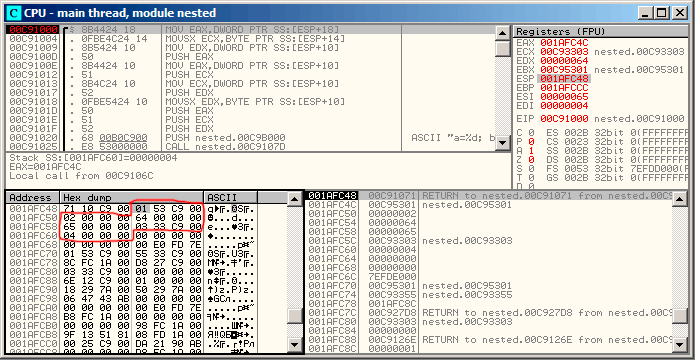
\includegraphics[scale=\FigScale]{patterns/15_structs/5_nested/olly.png}
\caption{\olly: Перед исполнением \printf}
\label{fig:nested_olly}
\end{figure}

Вот как расположены значения в памяти:
\begin{itemize}
\item \IT{(outer\_struct.a)} (байт) 1 + 3 байта случайного мусора;
\item \IT{(outer\_struct.b)} (32-битное слово) 2;
\item \IT{(inner\_struct.a)} (32-битное слово) 0x64 (100);
\item \IT{(inner\_struct.b)} (32-битное слово) 0x65 (101);
\item \IT{(outer\_struct.d)} (байт) 3 + 3 байта случайного мусора;
\item \IT{(outer\_struct.e)} (32-битное слово) 4.
\end{itemize}

}
\section{\RU{Работа с битовыми полями в структуре}\EN{Bit fields in a structure}}

\subsection{\RU{Пример CPUID}\EN{CPUID example}}

\RU{Язык \CCpp позволяет указывать, сколько именно бит отвести для каждого поля структуры. 
Это удобно если нужно экономить место в памяти. К примеру, для переменной типа \Tbool достаточно одного бита.
Но, это не очень удобно, если нужна скорость.}
\EN{\CCpp language allow to define exact number of bits for each structure fields.
It is very useful if one needs to save memory space. 
For example, one bit is enough for variable of \Tbool type.
But of course, it is not rational if speed is important.}

\newcommand{\FNCPUID}{\footnote{\url{http://en.wikipedia.org/wiki/CPUID}}}

\index{x86!\Instructions!CPUID}
\label{cpuid}
\RU{Рассмотрим пример с инструкцией \CPUID\FNCPUID. 
Эта инструкция возвращает информацию о том, какой процессор имеется в наличии и какие возможности он имеет.}
\EN{Let's consider \CPUID\FNCPUID instruction example.
This instruction returning information about current CPU and its features.}

\RU{Если перед исполнением инструкции в \EAX будет 1, 
то \CPUID вернет упакованную в \EAX такую информацию о процессоре:}
\EN{If the \EAX is set to 1 before instruction execution, 
\CPUID will return this information packed into the \EAX register:}

\begin{center}
\begin{tabular}{ | l | l | }
\hline
3:0 (4 \bitsENRU)& Stepping \\
7:4 (4 \bitsENRU) & Model \\
11:8 (4 \bitsENRU) & Family \\
13:12 (2 \bitsENRU) & Processor Type \\
19:16 (4 \bitsENRU) & Extended Model \\
27:20 (8 \bitsENRU) & Extended Family \\
\hline
\end{tabular}
\end{center}

\newcommand{\FNGCCAS}{\footnote{\href{http://www.ibiblio.org/gferg/ldp/GCC-Inline-Assembly-HOWTO.html}
{\RU{Подробнее о встроенном ассемблере GCC}\EN{More about internal GCC assembler}}}}

\RU{MSVC 2010 имеет макрос для \CPUID, а GCC 4.4.1 ~--- нет. 
Поэтому для GCC сделаем эту функцию сами, используя его встроенный ассемблер\FNGCCAS.}
\EN{MSVC 2010 has \CPUID macro, but GCC 4.4.1~---has not.
So let's make this function by yourself for GCC with the help of its built-in assembler\FNGCCAS.}

\lstinputlisting{patterns/15_structs/6_bitfields/cpuid/CPUID.c}

\RU{После того как \CPUID заполнит \EAX/\EBX/\ECX/\EDX, у нас они отразятся в массиве \TT{b[]}. 
Затем, мы имеем указатель на структуру \TT{CPUID\_1\_EAX}, и мы указываем его на значение 
\EAX из массива \TT{b[]}.}
\EN{After \CPUID will fill \EAX/\EBX/\ECX/\EDX, these registers will be reflected in the \TT{b[]} array.
Then, we have a pointer to the \TT{CPUID\_1\_EAX} structure and we point it to the value in the \EAX from \TT{b[]} array.}

\RU{Иными словами, мы трактуем 32-битный \Tint как структуру.}
\EN{In other words, we treat 32-bit \Tint value as a structure.}
\RU{Затем мы читаем из структуры.}\EN{Then we read from the stucture.}

\subsubsection{MSVC}

\RU{Компилируем в MSVC 2008 с опцией \Ox}\EN{Let's compile it in MSVC 2008 with \Ox option}:

\lstinputlisting[caption=\Optimizing MSVC 2008]{patterns/15_structs/6_bitfields/cpuid/CPUID_msvc_Ox.asm}

\index{x86!\Instructions!SHR}
\RU{Инструкция \TT{SHR} сдвигает значение из \EAX на то количество бит, 
которое нужно \IT{пропустить}, то есть, мы игнорируем некоторые биты \IT{справа}.}
\EN{\TT{SHR} instruction shifting value in the \EAX register by number of bits must be
\IT{skipped}, e.g., we ignore some bits \IT{at right}.}

\index{x86!\Instructions!AND}
\RU{А инструкция \ANDIns очищает биты \IT{слева} которые нам не нужны, или же, говоря иначе, 
она оставляет по маске только те биты в \EAX, которые нам сейчас нужны.}
\EN{\ANDIns instruction clears bits not needed \IT{at left}, or, in other words, 
leaves only those bits in the \EAX register we need now.}

\ifdefined\IncludeOlly
\subsubsection{MSVC + \olly}
\index{\olly}

\RU{Загрузим пример в}\EN{Let's load our example into} \olly 
\RU{и увидим, какие значения были установлены в EAX/EBX/ECX/EDX после
исполнения}\EN{and see, which values was set in EAX/EBX/ECX/EDX after execution of} CPUID: 
\figref{fig:cpuid_olly_1}.

\RU{В EAX установлено}\EN{EAX has} \TT{0x000206A7} 
(\RU{мой}\EN{my} \ac{CPU} \EN{is}\RU{---} Intel Xeon E3-1220).\\
\RU{В двоичном виде это}\EN{This is} $0000 0000 0000 0010 0000 0110 1010 0111$\EN{ in binary form}.

\RU{Вот как распределяются биты по полям в моем случае}\EN{Here is how bits are distributed by fields}:

\begin{center}
\begin{tabular}{ | l | l | l | }
\hline
\headercolor{} \RU{поле}\EN{field} &
\headercolor{} \RU{в двоичном виде}\EN{in binary form} &
\headercolor{} \RU{в десятичном виде}\EN{in decimal form} \\
\hline
reserved2		& 0000 & 0 \\
\hline
extended\_family\_id	& 00000000 & 0 \\
\hline
extended\_model\_id	& 0010 & 2 \\
\hline
reserved1		& 00 & 0 \\
\hline
processor\_id		& 00 & 0 \\
\hline
family\_id		& 0110 & 6 \\
\hline
model			& 1010 & 10 \\
\hline
stepping		& 0111 & 7 \\
\hline
\end{tabular}
\end{center}

\begin{figure}[H]
\centering
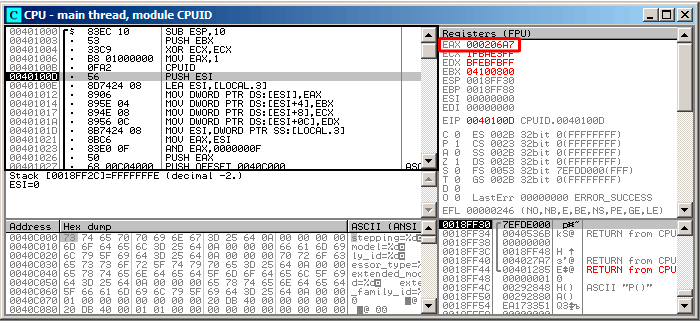
\includegraphics[scale=\FigScale]{patterns/15_structs/6_bitfields/cpuid/olly.png}
\caption{\olly: \RU{После исполнения CPUID}\EN{After CPUID execution}}
\label{fig:cpuid_olly_1}
\end{figure}

\begin{figure}[H]
\centering
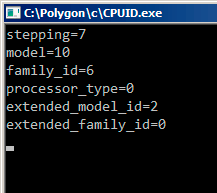
\includegraphics[scale=0.66]{patterns/15_structs/6_bitfields/cpuid/result.png}
\caption{\olly: \RU{Результат работы}\EN{Result}}
\label{fig:cpuid_olly_2}
\end{figure}
\fi

\subsubsection{GCC}

\RU{Попробуем GCC 4.4.1 с опцией \Othree.}\EN{Let's try GCC 4.4.1 with \Othree option.}

\lstinputlisting[caption=\Optimizing GCC 4.4.1]{patterns/15_structs/6_bitfields/cpuid/CPUID_gcc_O3.asm}

\RU{Практически, то же самое. Единственное что стоит отметить это то, что GCC решил зачем-то объединить 
вычисление \TT{extended\_model\_id} и \TT{extended\_family\_id} в один блок, 
вместо того чтобы вычислять их перед соответствующим вызовом \printf.}
\EN{Almost the same.
The only thing worth noting is the GCC somehow united calculation of
\TT{extended\_model\_id} and \TT{extended\_family\_id} into one block,
instead of calculating them separately, before corresponding each \printf call.}

\subsection{\WorkingWithFloatAsWithStructSubSubSectionName}
\label{sec:floatasstruct}

\RU{Как уже ранее указывалось в секции о FPU~(\myref{sec:FPU}), 
и \Tfloat и \Tdouble содержат в себе \IT{знак}, \IT{мантиссу} и \IT{экспоненту}. 
Однако, можем ли мы работать с этими полями напрямую? Попробуем с \Tfloat.}
\EN{As we already noted in the section about FPU~(\myref{sec:FPU}), 
both \Tfloat and \Tdouble types consist of a \IT{sign}, 
a \IT{significand} (or \IT{fraction}) and an \IT{exponent}.
But will we be able to work with these fields directly? Let's try this with \Tfloat.}

\input{float_IEEE754.tex}

\lstinputlisting{patterns/15_structs/6_bitfields/float/float.c.\LANG}

\RU{Структура \TT{float\_as\_struct} занимает в памяти столько же места сколько и \Tfloat, 
то есть 4 байта или 32 бита.}
\EN{The \TT{float\_as\_struct} structure occupies the same amount of  memory as \Tfloat, i.e., 4 bytes or 32 bits.}

\RU{Далее мы выставляем во входящем значении отрицательный знак, 
а также прибавляя двойку к экспоненте, мы тем 
самым умножаем всё значение на \TT{$2^2$}, то есть на 4.}
\EN{Now we are setting the negative sign in the input value and also, by adding 2 to the exponent, 
we thereby multiply the whole number by \TT{$2^2$}, i.e., by 4.}

\RU{Компилируем в MSVC 2008 без включенной оптимизации:}
\EN{Let's compile in MSVC 2008 without optimization turned on:}

\lstinputlisting[caption=\NonOptimizing MSVC 2008]{patterns/15_structs/6_bitfields/float/float_msvc.asm.\LANG}

\RU{Слегка избыточно. В версии скомпилированной с флагом \Ox нет вызовов \TT{memcpy()}, 
там работа происходит сразу с переменной \TT{f}. Но по неоптимизированной версии будет проще понять.}
\EN{A bit redundant.
If it was compiled with \Ox flag there would be no \TT{memcpy()} call,
the \TT{f} variable is used directly.
But it is easier to understand by looking at the unoptimized version.}

\RU{А что сделает GCC 4.4.1 с опцией \Othree?}\EN{What would GCC 4.4.1 with \Othree do?}

\lstinputlisting[caption=\Optimizing GCC 4.4.1]{patterns/15_structs/6_bitfields/float/float_gcc_O3.asm.\LANG}

\RU{Да, функция \ttf в целом понятна. Однако, что интересно, еще при компиляции, 
не взирая на мешанину с полями структуры, GCC умудрился вычислить результат функции \TT{f(1.234)} еще
во время компиляции и сразу подставить его в аргумент для \printf{}!}
\EN{The \ttf function is almost understandable. However, what is interesting is that GCC was able to calculate
the result of \TT{f(1.234)} during compilation despite all this hodge-podge with the structure fields
and prepared this argument to \printf{} as precalculated at compile time!}


\subsection{\Exercises}

\begin{itemize}
	\item \url{http://challenges.re/71}
	\item \url{http://challenges.re/72}
\end{itemize}





\chapter{\RU{Объединения (union)}\EN{Unions}}

\section{\IFRU{Пример генератора случайных чисел}{Pseudo-random number generator example}}

\IFRU{Если нам нужны случайные значения с плавающей запятой в интервале от 0 до 1, самое простое это взять
\ac{PRNG} вроде Mersenne twister выдающий случайные 32-битные числа в виде DWORD, преобразовать
это число в \Tfloat и затем разделить на \TT{RAND\_MAX} (\TT{0xFFFFFFFF} в данном случае) ~--- 
полученное число будет в интервале от 0 до 1.}
{If we need float random numbers from 0 to 1, the most simplest thing is to use \ac{PRNG} like
Mersenne twister produces random 32-bit values in DWORD form, transform this value to \Tfloat and then
dividing it by \TT{RAND\_MAX} (\TT{0xFFFFFFFF} in our case)~---value we got will be in 0..1 interval.}

\IFRU{Но как известно, операция деления ~--- это медленная операция. 
Сможем ли мы избежать её, как в случае с делением через умножение?}
{But as we know, division operation is slow.
Will it be possible to get rid of it, as in case of division by multiplication?}
~(\ref{sec:divisionbynine})

\index{IEEE 754}
\IFRU{Вспомним состав числа с плавающей запятой: это бит знака, биты мантиссы и биты экспоненты. 
Для получения случайного числа, нам нужно просто заполнить случайными битами все биты мантиссы!}
{Let's recall what float number consisted of: sign bit, significand bits and exponent bits.
We need just to store random bits to all significand bits for getting random float number!}

\IFRU{Экспонента не может быть нулевой (иначе число будет денормализованным), 
так что в эти биты мы запишем \TT{01111111} ~--- 
это будет означать что экспонента равна единице. Далее заполняем мантиссу случайными битами, 
знак оставляем в виде 0 (что значит наше число положительное), и вуаля. 
Генерируемые числа будут в интервале от 1 до 2, так что нам еще нужно будет отнять единицу.}
{Exponent cannot be zero (number will be denormalized in this case), so we will store \TT{01111111} 
to exponent~---this means exponent will be 1. Then fill significand with random bits, set sign bit to
0 (which means positive number) and voilà.
Generated numbers will be in 1 to 2 interval, so we also must subtract 1 from it.}

\newcommand{\URLXOR}{\url{http://xor0110.wordpress.com/2010/09/24/how-to-generate-floating-point-random-numbers-efficiently}}

\IFRU{В моем примере\footnote{идея взята здесь: \URLXOR} 
применяется очень простой линейный конгруэнтный генератор случайных чисел, выдающий 32-битные числа.
Генератор инициализируется текущим временем в стиле UNIX.}
{Very simple linear congruential random numbers generator is used in my 
example\footnote{idea was taken from: \URLXOR}, produces 32-bit numbers. 
The PRNG initializing by current time in UNIX-style.}

\IFRU{Далее, тип \Tfloat представляется в виде \IT{union} ~--- это конструкция \CCpp позволяющая 
интерпретировать часть памти по-разному. В нашем случае, мы можем создать переменную типа \TT{union} 
и затем обращаться к ней как к \Tfloat или как к \IT{uint32\_t}. Можно сказать, что это хак, причем грязный.}
{Then, \Tfloat type represented as \IT{union}~---it is the \CCpp construction enabling us
to interpret piece of memory as differently typed.
In our case, we are able to create a variable
of \TT{union} type and then access to it as it is \Tfloat or as it is \IT{uint32\_t}. 
It can be said, it is just a hack. A dirty one.}

\lstinputlisting{patterns/17_unions/FPU_PRNG.cpp}

\lstinputlisting[caption=MSVC 2010 (\Ox)]{patterns/17_unions/FPU_PRNG_msvc_2010_Ox_\LANG.asm}

\IFRU{А результат GCC будет почти таким же.}{GCC produces very similar code.}



\newcommand{\comp}{\TT{comp()}\xspace}
\chapter{\RU{Указатели на функции}\EN{Pointers to functions}}
\label{sec:pointerstofunctions}

\index{\CLanguageElements!\Pointers}
\RU{Указатель на функцию, в целом, как и любой другой указатель, просто адрес указывающий на начало функции 
в сегменте кода.}
\EN{Pointer to function, as any other pointer, is just an address of function beginning in its code segment.}

\index{Callbacks}
\RU{Это применяется часто в т.н. callback-ах}\EN{It is often used in callbacks}
\footnote{\url{http://en.wikipedia.org/wiki/Callback_(computer_science)}}.

\RU{Известные примеры:}\EN{Well-known examples are:}

\begin{itemize}
\item
\qsort\footnote{\url{http://en.wikipedia.org/wiki/Qsort_(C_standard_library)}},
{\TT{atexit()}}\footnote{\url{http://www.opengroup.org/onlinepubs/009695399/functions/atexit.html}} \RU{из стандартной библиотеки Си}\EN{from the standard C library}; 
\item
\RU{сигналы в *NIX ОС}\EN{signals in *NIX OS}\footnote{\url{http://en.wikipedia.org/wiki/Signal.h}};
\item
\RU{запуск тредов}\EN{thread starting}: \TT{CreateThread()} (win32), \TT{pthread\_create()} (POSIX);
\item
\RU{множество функций win32, например}\EN{a lot of win32 functions, e.g.} \TT{EnumChildWindows()}\footnote{\url{http://msdn.microsoft.com/en-us/library/ms633494(VS.85).aspx}}.
\end{itemize}

\index{\CStandardLibrary!qsort()}
\RU{Итак, функция \qsort это реализация алгоритма ``быстрой сортировки''. 
Функция может сортировать что угодно, 
любые типы данных, но при условии, что вы имеете функцию сравнения двух элементов данных и 
\qsort может вызывать её.}
\EN{So, \qsort function is a \CCpp standard library quicksort implementation. The functions is able to sort
anything, any types of data, if you have a function for two elements comparison and \qsort is able
to call it.}

\RU{Эта функция сравнения может определяться так:}\EN{The comparison function can be defined as:}

\begin{lstlisting}
int (*compare)(const void *, const void *)
\end{lstlisting}

\RU{Воспользуемся немного модифицированным примером, который я нашел вот}
\EN{Let's use slightly modified example I found} \href{http://cplus.about.com/od/learningc/ss/pointers2_8.htm}
{\RU{здесь}\EN{here}}:

\lstinputlisting[numbers=left,label=qsort_c_src]{patterns/18_pointers_to_functions/17_1.c}

\section{MSVC}

\RU{Компилируем в MSVC 2010 (я убрал некоторые части для краткости) с опцией \Ox}
\EN{Let's compile it in MSVC 2010 (I omitted some parts for the sake of brevity) with \Ox option}:

\lstinputlisting[caption=\Optimizing MSVC 2010: /Ox /GS- /MD]{patterns/18_pointers_to_functions/17_2_msvc_Ox.asm}

\RU{Ничего особо удивительного здесь мы не видим. В качестве четвертого аргумента, 
в \qsort просто передается адрес метки \TT{\_comp}, где собственно и располагается функция \comp.}
\EN{Nothing surprising so far.
As a fourth argument, an address of label \TT{\_comp} is passed, that is just a place
where function \comp located.}

\RU{Как \qsort вызывает её?}\EN{How \qsort calling it?}

\index{Windows!MSVCR80.DLL}
\RU{Посмотрим в MSVCR80.DLL (эта DLL куда в MSVC вынесены функции из стандартных библиотек Си):}
\EN{Let's take a look into this function located in MSVCR80.DLL (a MSVC DLL module with C standard library functions):}

\lstinputlisting[caption=MSVCR80.DLL]{patterns/18_pointers_to_functions/17_3_MSVCR.lst}

\TT{comp}\EMDASH{}\RU{это четвертый аргумент функции. 
Здесь просто передается управление по адресу указанному в \TT{comp}. 
Перед этим подготавливается два аргумента для функции \comp. 
Далее, проверяется результат её выполнения.}
\EN{is fourth function argument.
Here the control is just passed to the address in the \TT{comp} argument.
Before it, two arguments prepared for \comp. Its result is checked after its execution.}

\RU{Вот почему использование указателей на функции ~--- это опасно. 
Во-первых, если вызвать \qsort с неправильным указателем на функцию, 
то \qsort, дойдя до этого вызова, может передать управление неизвестно куда, 
процесс упадет, и эту ошибку можно будет найти не сразу.}
\EN{That's why it is dangerous to use pointers to functions.
First of all, if you call \qsort with incorrect pointer to function, \qsort may pass control
to incorrect point, a process may crash and this bug will be hard to find.}

\RU{Во-вторых, типизация callback-функции должна строго соблюдаться, 
вызов не той функции с не теми аргументами не того типа, 
может привести к плачевным результатам, 
хотя падение процесса это и не проблема, проблема ~--- это найти ошибку, ведь компилятор 
на стадии компиляции может вас и не предупредить о потенциальных неприятностях.}
\EN{Second reason is the callback function types must comply strictly, calling wrong function
with wrong arguments of wrong types may lead to serious problems, however, process crashing is not a 
big problem~---big problem is to determine a reason of crashing~---because compiler may be 
silent about potential trouble while compiling.}

\subsection{MSVC + \olly}
\index{\olly}

\RU{Загрузим наш пример в \olly и установим брякпойнт на ф-ции \comp}
\EN{Let's load our example into \olly and set breakpoint on \comp function}.

\RU{Как значения сравниваются, мы можем увидеть во время самого первого вызова \comp}
\EN{How values are compared we can see at the very first \comp call}: \figname \ref{fig:qsort_olly1}.
\RU{Для удобства, }\olly \RU{показывает сравниваемые значения в окне под окном кода}
\EN{shows compared values in the window under code window, for convenience}.
\RU{Мы можем так же увидеть что}\EN{We can also see that the} \ac{SP} \RU{указывает на}\EN{pointing to} 
\ac{RA} \RU{где находится место в ф-ции}\EN{where the place in} 
\qsort \EN{function is }(\RU{на самом деле, находится в}\EN{actually located in} \TT{MSVCR100.DLL}).

\RU{Трассируя}\EN{By tracing} (F8) \RU{до инструкции}\EN{until} \TT{RETN} 
\RU{и нажав F8 еще один раз, мы возвращаемся в ф-цию}\EN{instruction, and pressing F8 one more time, 
we returning into} \qsort\EN{ function}: \figname \ref{fig:qsort_olly2}.
\RU{Это был вызов ф-ции сравнения}\EN{That was a call to comparison function}.

\RU{Вот также скриншот момента второго вызова ф-ции}\EN{Here is also screenshot of the moment of the 
second call of} \comp\EMDASH{}\RU{теперь сравниваемые значения другие}
\EN{now values to be compared are different}:
\figname \ref{fig:qsort_olly3}.

\begin{figure}[H]
\centering
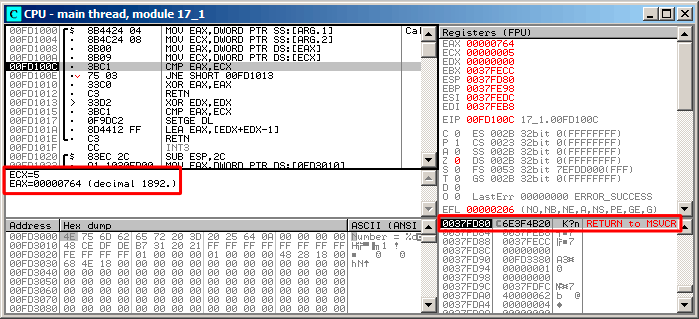
\includegraphics[scale=\FigScale]{patterns/18_pointers_to_functions/olly1.png}
\caption{\olly: \RU{первый вызов}\EN{first call of} \comp}
\label{fig:qsort_olly1}
\end{figure}

\begin{figure}[H]
\centering
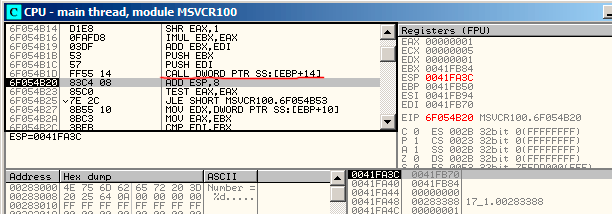
\includegraphics[scale=\FigScale]{patterns/18_pointers_to_functions/olly2.png}
\caption{\olly: \RU{код в}\EN{the code in} \qsort \RU{сразу после вызова}\EN{right after} \comp\EN{ call}}
\label{fig:qsort_olly2}
\end{figure}

\begin{figure}[H]
\centering
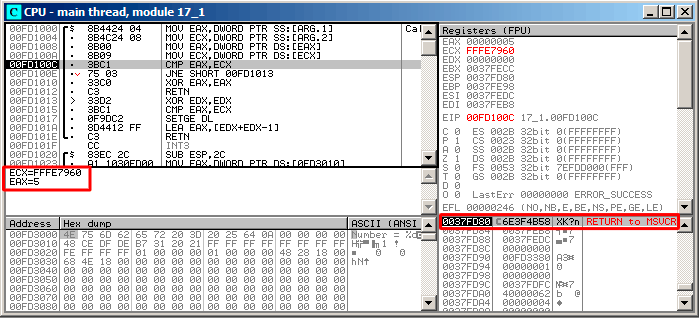
\includegraphics[scale=\FigScale]{patterns/18_pointers_to_functions/olly3.png}
\caption{\olly: \RU{второй вызов}\EN{second call of} \comp}
\label{fig:qsort_olly3}
\end{figure}

\subsection{MSVC + tracer}
\index{tracer}

\RU{Посмотрим, какие пары сравниваются}\EN{Let's also see, which pairs are compared}.
\RU{Эти 10 чисел будут сортироваться}\EN{These 10 numbers are being sorted}: 
1892, 45, 200, -98, 4087, 5, -12345, 1087, 88, -100000.

\RU{Я нашел адрес первой инструкции}\EN{I found the address of the first} \CMP 
\RU{в}\EN{instruction in} \comp, \RU{и это}\EN{it is} \TT{0x0040100C} 
\RU{и я ставлю брякпойнт на нем}\EN{and I'm setting breakpoint on it}:

\begin{lstlisting}
tracer.exe -l:17_1.exe bpx=17_1.exe!0x0040100C
\end{lstlisting}

\RU{Получаю информацию о регистрах на брякпойнте}
\EN{I'm getting information about registers at breakpoint}:

\begin{lstlisting}
PID=4336|New process 17_1.exe
(0) 17_1.exe!0x40100c
EAX=0x00000764 EBX=0x0051f7c8 ECX=0x00000005 EDX=0x00000000
ESI=0x0051f7d8 EDI=0x0051f7b4 EBP=0x0051f794 ESP=0x0051f67c
EIP=0x0028100c
FLAGS=IF
(0) 17_1.exe!0x40100c
EAX=0x00000005 EBX=0x0051f7c8 ECX=0xfffe7960 EDX=0x00000000
ESI=0x0051f7d8 EDI=0x0051f7b4 EBP=0x0051f794 ESP=0x0051f67c
EIP=0x0028100c
FLAGS=PF ZF IF
(0) 17_1.exe!0x40100c
EAX=0x00000764 EBX=0x0051f7c8 ECX=0x00000005 EDX=0x00000000
ESI=0x0051f7d8 EDI=0x0051f7b4 EBP=0x0051f794 ESP=0x0051f67c
EIP=0x0028100c
FLAGS=CF PF ZF IF
...
\end{lstlisting}

\RU{Я отфильтровал}\EN{I filtered out} \TT{EAX} \AndENRU \TT{ECX} \RU{и получил}\EN{and got}:

\begin{lstlisting}
EAX=0x00000764 ECX=0x00000005
EAX=0x00000005 ECX=0xfffe7960
EAX=0x00000764 ECX=0x00000005
EAX=0x0000002d ECX=0x00000005
EAX=0x00000058 ECX=0x00000005
EAX=0x0000043f ECX=0x00000005
EAX=0xffffcfc7 ECX=0x00000005
EAX=0x000000c8 ECX=0x00000005
EAX=0xffffff9e ECX=0x00000005
EAX=0x00000ff7 ECX=0x00000005
EAX=0x00000ff7 ECX=0x00000005
EAX=0xffffff9e ECX=0x00000005
EAX=0xffffff9e ECX=0x00000005
EAX=0xffffcfc7 ECX=0xfffe7960
EAX=0x00000005 ECX=0xffffcfc7
EAX=0xffffff9e ECX=0x00000005
EAX=0xffffcfc7 ECX=0xfffe7960
EAX=0xffffff9e ECX=0xffffcfc7
EAX=0xffffcfc7 ECX=0xfffe7960
EAX=0x000000c8 ECX=0x00000ff7
EAX=0x0000002d ECX=0x00000ff7
EAX=0x0000043f ECX=0x00000ff7
EAX=0x00000058 ECX=0x00000ff7
EAX=0x00000764 ECX=0x00000ff7
EAX=0x000000c8 ECX=0x00000764
EAX=0x0000002d ECX=0x00000764
EAX=0x0000043f ECX=0x00000764
EAX=0x00000058 ECX=0x00000764
EAX=0x000000c8 ECX=0x00000058
EAX=0x0000002d ECX=0x000000c8
EAX=0x0000043f ECX=0x000000c8
EAX=0x000000c8 ECX=0x00000058
EAX=0x0000002d ECX=0x000000c8
EAX=0x0000002d ECX=0x00000058
\end{lstlisting}

\RU{Это}\EN{That's} 34 \RU{пары}\EN{pairs}.
\RU{Следовательно, алгоритму быстрой сортировки нужно 34 операции сравнения для сортировки этих
10-и чисел}\EN{Therefore, quick sort algorithm needs 34 comparison operations for sorting these 10 numbers}.

\subsection{MSVC + tracer (code coverage)}
\index{tracer}

\RU{Но можно также и воспользоваться возможностью tracer накапливать все возможные состояния регистров
и показать их в \IDA}\EN{We can also use tracer's feature to collect all possible register's values
and show them in \IDA}.

\RU{Трассируем все инструкции в ф-ции \comp}\EN{Let's trace all instructions in \comp function}:

\begin{lstlisting}
tracer.exe -l:17_1.exe bpf=17_1.exe!0x00401000,trace:cc
\end{lstlisting}

\RU{Получем .idc-скрипт для загрузки в \IDA и загружаем его}
\EN{We getting .idc-script for loading into \IDA and load it}: \figname \ref{fig:qsort_tracer_cc}.

\RU{Имя этой ф-ции (PtFuncCompare) дала \IDA}\EN{\IDA gave the function name (PtFuncCompare)}
\EMDASH{}\RU{видимо, потому что видит что указатель на эту ф-цию передается в \qsort}\EN{it seems,
because \IDA sees that pointer to this function is passed into \qsort}.

\RU{Мы видим что указатели $a$ и $b$ указывают на разные места внутри массива, 
но шаг между указателями --- 4, что логично, ведь в массиве хранятся 32-битные значения}
\EN{We see that $a$ and $b$ pointers are points to various places in array, but step between
points is 4---indeed, 32-bit values are stored in the array}.

\RU{Видно что инструкции по адресам}\EN{We see that the instructions at} \TT{0x401010} \AndENRU 
\TT{0x401012} \RU{никогда не исполнялись}\EN{was never executed} 
(\RU{они и остались белыми}\EN{so they leaved as white}): 
\RU{действительно, ф-ция}\EN{indeed,} \comp \RU{никогда не возвращала 0,
потому что в массиве нет одинаковых элементов}\EN{was never returned 0, because there no equal elements}.

\begin{figure}[H]
\centering
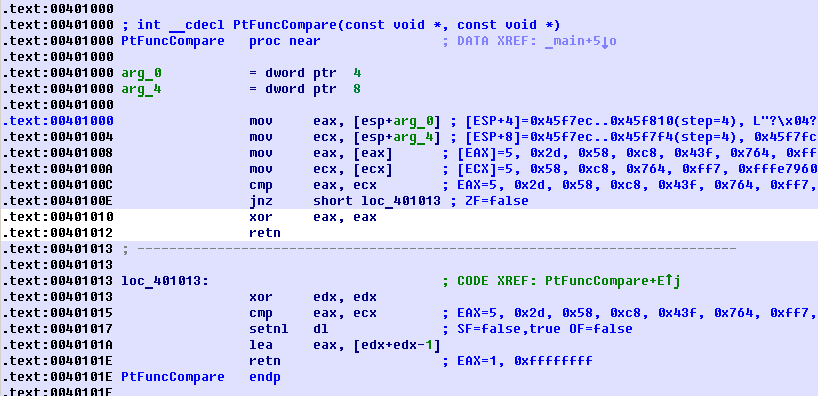
\includegraphics[scale=\FigScale]{patterns/18_pointers_to_functions/tracer_cc.png}
\caption{tracer \AndENRU IDA. N.B.: 
\RU{некоторые значения обрезаны справа}\EN{some values are cutted at right}}
\label{fig:qsort_tracer_cc}
\end{figure}

\section{GCC}

\RU{Не слишком большая разница}\EN{Not a big difference}:

\begin{lstlisting}[caption=GCC]
                lea     eax, [esp+40h+var_28]
                mov     [esp+40h+var_40], eax
                mov     [esp+40h+var_28], 764h
                mov     [esp+40h+var_24], 2Dh
                mov     [esp+40h+var_20], 0C8h
                mov     [esp+40h+var_1C], 0FFFFFF9Eh
                mov     [esp+40h+var_18], 0FF7h
                mov     [esp+40h+var_14], 5
                mov     [esp+40h+var_10], 0FFFFCFC7h
                mov     [esp+40h+var_C], 43Fh
                mov     [esp+40h+var_8], 58h
                mov     [esp+40h+var_4], 0FFFE7960h
                mov     [esp+40h+var_34], offset comp
                mov     [esp+40h+var_38], 4
                mov     [esp+40h+var_3C], 0Ah
                call    _qsort
\end{lstlisting}

\RU{Функция \comp}\EN{\comp function}:

\begin{lstlisting}
                public comp
comp            proc near

arg_0           = dword ptr  8
arg_4           = dword ptr  0Ch

                push    ebp
                mov     ebp, esp
                mov     eax, [ebp+arg_4]
                mov     ecx, [ebp+arg_0]
                mov     edx, [eax]
                xor     eax, eax
                cmp     [ecx], edx
                jnz     short loc_8048458
                pop     ebp
                retn
loc_8048458:
                setnl   al
                movzx   eax, al
                lea     eax, [eax+eax-1]
                pop     ebp
                retn
comp            endp
\end{lstlisting}

\index{Linux!libc.so.6}
\RU{Реализация \qsort находится в \TT{libc.so.6}, и представляет собой просто wrapper
\footnote{понятие близкое к \gls{thunk function}} для \TT{qsort\_r()}.}
\EN{\qsort implementation is located in the \TT{libc.so.6} and it is in fact just a wrapper
\footnote{a concept like \gls{thunk function}} for \TT{qsort\_r()}.}

\RU{Она, в свою очередь, вызывает \TT{quicksort()}, где есть вызовы определенной нами функции через 
переданный указатель:}
\EN{It will call then \TT{quicksort()}, where our defined function will be called via passed pointer:}


\begin{lstlisting}[caption=
(\RU{файл libc.so.6, версия glibc}\EN{file libc.so.6, glibc version}\EMDASH{}2.10.1)]

.text:0002DDF6                 mov     edx, [ebp+arg_10]
.text:0002DDF9                 mov     [esp+4], esi
.text:0002DDFD                 mov     [esp], edi
.text:0002DE00                 mov     [esp+8], edx
.text:0002DE04                 call    [ebp+arg_C]
...
\end{lstlisting}

\subsection{GCC + GDB (\RU{с исходными кодами}\EN{with source code})}
\index{GDB}

\RU{Очевидно, у нас есть исходный код нашего примера на Си (\ref{qsort_c_src}), 
так что мы можем установить брякпойнт (\TT{b}) на
номере строки}\EN{Obviously, we have a C-source code of our example (\ref{qsort_c_src}), 
so we can set breakpoint (\TT{b}) on line number}
(\RU{11-й --- это номер строки где происходит первое сравнение}\EN{11th---the line where 
first comparison is occurred}).
\RU{Нам также нужно скомпилировать наш пример с ключом \TT{-g}, чтобы в исполняемом файле была
полная отладочная информация}\EN{We also need to compile example with debugging information 
included (\TT{-g}), so the table
with addresses and corresponding line numbers is present}.
\RU{Мы можем так же выводить значения используя имена переменных}
\EN{We can also print values by variable name} (\TT{p}):
\RU{отладочная информация также содержит информацию о том, в каком регистре и/или элементе локального
стека находится какая переменная}\EN{debugging information also has information about which register and/or 
local stack element contain which variable}.

\index{Glibc}
\RU{Мы можем также увидеть стек}\EN{We can also see stack} (\TT{bt}) 
\RU{и обнаружить что в Glibc используется какая-то вспомогательная ф-ция с именем}
\EN{and find out that there are some intermediate function} 
\TT{msort\_with\_tmp()}\EN{ used in Glibc}.

\lstinputlisting[caption=GDB\RU{-сессия}\EN{ session}]{patterns/18_pointers_to_functions/GDB_source.txt}

\subsection{GCC + GDB (\RU{без исходных кодов}\EN{no source code})}
\index{GDB}

\RU{Но часто никаких исходных кодов нет вообще, так что мы можем дизассемблировать ф-цию \comp}
\EN{But often there are no source code at all, so we can disassemble \comp function} (\TT{disas}), 
\RU{найти самую первую инструкцию \CMP и установить брякпойнт}\EN{find the very first
\CMP instruction and set breakpoint} (\TT{b}) \RU{по этому адресу}\EN{at that address}.
\RU{На каждом брякпойнте мы будем видеть содержимое регистров}
\EN{At each breakpoint, we will dump all register contents} (\TT{info registers}).
\RU{Информация из стека так же доступна}\EN{Stack information is also available} (\TT{bt}), 
\RU{но частичная: здесь нет номеров строк для ф-ции \comp}
\EN{but partial: there are no line number information for \comp function}.

\lstinputlisting[caption=GDB\RU{-сессия}\EN{ session}]{patterns/18_pointers_to_functions/GDB_no_source.txt}


\ifdefined\ENGLISH
\section{64-bit values in 32-bit environment}
\label{sec:64bit_in_32_env}

In a 32-bit environment, \ac{GPR}'s are 32-bit, so 64-bit values are stored and passed as 32-bit value pairs
\footnote{By the way, 32-bit values are passed as pairs in 16-bit environment in the same way: \myref{win16_32bit_values}}.
\fi

\ifdefined\RUSSIAN
\section{64-битные значения в 32-битной среде}
\label{sec:64bit_in_32_env}

В среде, где \ac{GPR}-ы 32-битные, 64-битные значения хранятся и передаются как пары 32-битных значений
\footnote{Кстати, в 16-битной среде, 32-битные значения передаются 16-битными парами точно так же: \myref{win16_32bit_values}}.
\fi

\section{\RU{Возврат 64-битного значения}\EN{Returning of 64-bit value}}

\lstinputlisting{patterns/185_64bit_in_32_env/ret/0.c}

\subsection{x86}

\RU{64-битные значения в 32-битной среде возвращаются из ф-ций в паре регистров \EDX{}:\EAX{}.}
\EN{In a 32-bit environment, 64-bit values are returned from functions in the \EDX{}:\EAX{} register pair.}

\lstinputlisting[caption=\Optimizing MSVC 2010]{patterns/185_64bit_in_32_env/ret/0_MSVC_2010_Ox.asm}

\ifdefined\IncludeARM
\subsection{ARM}

\RU{64-битное значение возвращается в паре регистров R0-R1 ---
(R1 это старшая часть и R0 --- младшая часть):}
\EN{A 64-bit value is returned in the R0-R1 register pair 
(R1 is for the high part and R0 for the low part):}

\lstinputlisting[caption=\OptimizingKeilVI (\ARMMode)]{patterns/185_64bit_in_32_env/ret/Keil_ARM_O3.s}

\fi

\ifdefined\IncludeMIPS
\subsection{MIPS}

\RU{64-битное значение возвращается в паре регистров V0-V1 (\$2-\$3) ---
(V0 (\$2) это старшая часть и V1 (\$3) --- младшая часть):}
\EN{A 64-bit value is returned in the V0-V1 (\$2-\$3) register pair 
(V0 (\$2) is for the high part and V1 (\$3) for the low part):}

\lstinputlisting[caption=\Optimizing GCC 4.4.5 (assembly listing)]{patterns/185_64bit_in_32_env/ret/0_MIPS.s}

\lstinputlisting[caption=\Optimizing GCC 4.4.5 (IDA)]{patterns/185_64bit_in_32_env/ret/0_MIPS_IDA.lst}
\fi

\section{\RU{Передача аргументов, сложение, вычитание}\EN{Arguments passing, addition, subtraction}}

\lstinputlisting{patterns/185_64bit_in_32_env/passing_add_sub/1.c}

\subsection{x86}

\lstinputlisting[caption=\Optimizing MSVC 2012 /Ob1]{patterns/185_64bit_in_32_env/passing_add_sub/1_MSVC.asm}

\RU{В}\EN{We can see in the} \GTT{f\_add\_test()} \RU{видно, как каждое 64-битное число передается двумя 32-битными значениями,
сначала старшая часть, затем младшая}\EN{function that each 64-bit value is passed using two 32-bit values,
high part first, then low part}. \\
\\
\RU{Сложение и вычитание происходит также парами}\EN{Addition and subtraction occur in pairs as well}. \\
\\
\myindex{x86!\Instructions!ADC}
\RU{При сложении, в начале складываются младшие 32 бита}\EN{In addition, the low 32-bit part are added first}.
\RU{Если при сложении был перенос, выставляется флаг CF}\EN{If carry was occurred while adding, the CF flag is set}.
\RU{Следующая инструкция \INS{ADC} складывает старшие части чисел, но также прибавляет единицу если $CF=1$}
\EN{The following \INS{ADC} instruction adds the high parts of the values, and also adds 1 if $CF=1$}. \\
\\
\myindex{x86!\Instructions!SBB}
\RU{Вычитание также происходит парами}\EN{Subtraction also occurs in pairs}.
\RU{Первый}\EN{The first} \SUB \RU{может также включить флаг переноса CF, который затем будет проверяться в \INS{SBB}}
\EN{may also turn on the CF flag, which is to be checked in the subsequent \INS{SBB} instruction}:
\RU{если флаг переноса включен, то от результата отнимется единица}
\EN{if the carry flag is on, then 1 is also to be subtracted from the result}. \\
\\
\RU{Легко увидеть, как результат работы \GTT{f\_add()} затем передается в \printf{}}\EN{It is easy to see how
the \GTT{f\_add()} function result is then passed to \printf{}}.

\ifdefined\IncludeGCC
\lstinputlisting[caption=GCC 4.8.1 -O1 -fno-inline]{patterns/185_64bit_in_32_env/passing_add_sub/1_GCC.asm}

\RU{Код GCC почти такой же}\EN{GCC code is the same}.
\fi

\ifdefined\IncludeARM
\subsection{ARM}

\lstinputlisting[caption=\OptimizingKeilVI (\ARMMode)]{patterns/185_64bit_in_32_env/passing_add_sub/Keil_ARM_O3.s}

\myindex{ARM!\Instructions!ADDS}
\myindex{ARM!\Instructions!SUBS}
\myindex{ARM!\Instructions!ADC}
\myindex{ARM!\Instructions!SBC}
\RU{Первое 64-битное значение передается в паре регистров R0 и R1, второе --- в паре R2 и R3.}
\EN{The first 64-bit value is passed in R0 and R1 register pair, the second in R2 and R3 register pair.}
\RU{В ARM также есть инструкция ADC (учитывающая флаг переноса) и SBC (\q{subtract with carry} --- вычесть
с переносом).}
\EN{ARM has the ADC instruction as well (which counts carry flag) and SBC (\q{subtract with carry}).}

\RU{Важная вещь: когда младшие части слагаются/вычитаются, используются инструкции ADDS и SUBS с суффиксом
-S.}
\EN{Important thing: when the low parts are added/subtracted, ADDS and SUBS instructions with -S suffix are used.}
\RU{Суффикс -S означает \q{set flags} (установить флаги), а флаги (особенно флаг переноса) это то что однозначно
нужно последующим инструкциями ADC/SBC.}
\EN{The -S suffix stands for \q{set flags}, and flags (esp. carry flag) is what consequent ADC/SBC instructions
definitely need.}

\RU{А иначе инструкции без суффикса -S здесь вполне бы подошли (ADD и SUB).}
\EN{Otherwise, instructions without the -S suffix would do the job (ADD and SUB).}

\fi

\ifdefined\IncludeMIPS
\subsection{MIPS}

\lstinputlisting[caption=\Optimizing GCC 4.4.5 (IDA)]{patterns/185_64bit_in_32_env/passing_add_sub/MIPS_O3_IDA.lst.\LANG}

\RU{В MIPS нет регистра флагов, так что эта информация не присутствует после исполнения арифметических операций.}
\EN{MIPS has no flags register, so there is no such information present after the execution of arithmetic operations.}
\EN{So there are no instructions like x86's ADC and SBB.}
\RU{Так что здесь нет инструкций как ADC или SBB в x86.}
\RU{Чтобы получить информацию о том, был бы выставлен флаг переноса, происходит сравнение (используя инструкцию
\q{SLTU}), которая выставляет целевой регистр в 1 или 0.}
\EN{To know if the carry flag would be set, a comparison (using \q{SLTU} instruction) also occurs, 
which sets the destination register to 1 or 0.}
\RU{Эта 1 или 0 затем прибавляется к итоговому результату, или вычитается.}
\EN{This 1 or 0 is then added or subtracted to/from the final result.}

\fi

\section{\RU{Умножение, деление}\EN{Multiplication, division}}

\lstinputlisting{patterns/185_64bit_in_32_env/multdiv/2.c}

\subsection{x86}

\lstinputlisting[caption=\Optimizing MSVC 2012 /Ob1]{patterns/185_64bit_in_32_env/multdiv/2_MSVC.asm.\LANG}

\RU{Умножение и деление --- это более сложная операция, так что обычно, компилятор встраивает вызовы библиотечных функций,
делающих это}\EN{Multiplication and division are more complex operations, so usually the compiler embeds calls to
a library functions doing that}.

\ifx\LITE\undefined
\RU{Значение этих библиотечных функций, здесь}\EN{These functions are described here}: \myref{sec:MSVC_library_func}.
\fi

\ifdefined\IncludeGCC
\lstinputlisting[caption=\Optimizing GCC 4.8.1 -fno-inline]{patterns/185_64bit_in_32_env/multdiv/2_GCC.asm.\LANG}

\RU{GCC делает почти то же самое, тем не менее,
встраивает код умножения прямо в функцию, посчитав что так будет эффективнее}\EN{GCC does the expected, but the multiplication
code is inlined right in the function, thinking it could be more efficient}.
\RU{У GCC другие имена библиотечных функций}\EN{GCC has different library function names}: \myref{sec:GCC_library_func}.
\fi

\ifdefined\IncludeARM
\subsection{ARM}

\RU{Keil для режима Thumb вставляет вызовы библиотечных функций:}
\EN{Keil for Thumb mode inserts library subroutine calls:}

\lstinputlisting[caption=\OptimizingKeilVI (\ThumbMode)]{patterns/185_64bit_in_32_env/multdiv/Keil_thumb_O3.s}

\RU{Keil для режима ARM, тем не менее, может сгенерировать код для умножения 64-битных чисел:}
\EN{Keil for ARM mode, on the other hand, is able to produce 64-bit multiplication code:}

\lstinputlisting[caption=\OptimizingKeilVI (\ARMMode)]{patterns/185_64bit_in_32_env/multdiv/Keil_ARM_O3.s}
% TODO add explanation
\fi

\ifdefined\IncludeMIPS
\subsection{MIPS}

\Optimizing GCC \ForENRU MIPS 
\EN{can generate 64-bit multiplication code, but has to call a library routine for 64-bit division:}
\RU{может генерировать код для 64-битного умножения, но для 64-битного деления приходится вызывать библиотечную функцию:}

\lstinputlisting[caption=\Optimizing GCC 4.4.5 (IDA)]{patterns/185_64bit_in_32_env/multdiv/MIPS_O3_IDA.lst}

\RU{Тут также много \ac{NOP}-ов, это возможно заполнение delay slot-ов после инструкции умножения (она ведь работает
медленнее прочих инструкций), но я не однозначно уверен.}
\EN{There are a lot of \ac{NOP}s, probably delay slots filled after the multiplication instruction (it's slower
than other instructions, after all), but I'm not completely sure.}

% TODO add explanation
\fi

\section{\RU{Сдвиг вправо}\EN{Shifting right}}

\lstinputlisting{patterns/185_64bit_in_32_env/shifting/3.c}

\subsection{x86}

\lstinputlisting[caption=\Optimizing MSVC 2012 /Ob1]{patterns/185_64bit_in_32_env/shifting/3_MSVC.asm}

\ifdefined\IncludeGCC
\lstinputlisting[caption=\Optimizing GCC 4.8.1 -fno-inline]{patterns/185_64bit_in_32_env/shifting/3_GCC.asm}
\fi

\index{x86!\Instructions!SHRD}
\RU{Сдвиг происходит также в две операции: в начале сдвигается младшая часть, затем старшая}
\EN{Shifting also occurs in two passes: first the lower part is shifted, then the higher part}.
\RU{Но младшая часть сдвигается
при помощи инструкции \INS{SHRD}, она сдвигает значение в \EDX{} на 7 бит, но подтягивает новые биты из \EAX{}, т.е. из старшей части.}
\EN{But the lower part is shifted with the help of the \INS{SHRD} instruction, it shifts the value of \EDX{} by 7 bits, but pulls new bits
from \EAX{}, i.e., from the higher part.}
\RU{Старшая часть сдвигается более известной инструкцией \SHR{}: действительно, ведь освободившиеся биты в старшей части нужно
просто заполнить нулями}\EN{The higher part is shifted using the more popular \SHR{} instruction: indeed, the freed bits in the higher part
must be filled with zeroes}.

\ifdefined\IncludeARM
\subsection{ARM}

\RU{В ARM нет такой инструкции как SHRD в x86, так что компилятору Keil приходится всё это делать,
используя простые сдвиги и операции \q{ИЛИ}:}
\EN{ARM doesn't have such instruction as SHRD in x86, so the Keil compiler ought to do this using simple shifts
and OR operations:}

\lstinputlisting[caption=\OptimizingKeilVI (\ARMMode)]{patterns/185_64bit_in_32_env/shifting/Keil_ARM_O3.s}

\lstinputlisting[caption=\OptimizingKeilVI (\ThumbMode)]{patterns/185_64bit_in_32_env/shifting/Keil_thumb_O3.s}
% TODO add explanation
\fi

\ifdefined\IncludeMIPS
\subsection{MIPS}

\ifdefined\IncludeGCC
\EN{GCC for MIPS follows the same algorithm as Keil does for Thumb mode:}
\RU{GCC для MIPS реализует тот же алгоритм, что сделал Keil для режима Thumb:}

\lstinputlisting[caption=\Optimizing GCC 4.4.5 (IDA)]{patterns/185_64bit_in_32_env/shifting/MIPS_O3_IDA.lst}
\fi

% TODO add explanation
\fi

\section{\RU{Конвертирование 32-битного значения в 64-битное}\EN{Converting 32-bit value into 64-bit one}}
\label{subsec:sign_extending_32_to_64}

\lstinputlisting{patterns/185_64bit_in_32_env/conversion/4.c}

\subsection{x86}

\lstinputlisting[caption=\Optimizing MSVC 2012]{patterns/185_64bit_in_32_env/conversion/MSVC2012_Ox.asm}

\RU{Здесь появляется необходимость расширить 32-битное знаковое значение в 64-битное знаковое.}
\EN{Here we also run into necessity to extend a 32-bit signed value into a 64-bit signed one.}
\RU{Конвертировать беззнаковые значения очень просто: нужно просто выставить в 0 все биты в старшей части}
\EN{Unsigned values are converted straightforwardly: all bits in the higher part must be set to 0}.
\RU{Но для знаковых типов это не подходит: знак числа должен быть скопирован в старшую часть числа-результата}
\EN{But this is not appropriate for signed data types: the sign has to be copied into the higher part of the resulting number}.
\myindex{x86!\Instructions!CDQ}
\RU{Здесь это делает инструкция \INS{CDQ}, она берет входное значение в \EAX{}, расширяет его до 64-битного,
и оставляет его в паре регистров \EDX{}:\EAX{}}
\EN{The \INS{CDQ} instruction does that here, it takes its input value in \EAX{}, extends it to 64-bit and leaves it
in the \EDX{}:\EAX{} register pair}.
\RU{Иными словами, инструкция \INS{CDQ} узнает знак числа в \EAX{} (просто берет самый старший бит в \EAX{}) и в зависимости от этого,
выставляет все 32 бита в \EDX{} в 0 или в 1}\EN{In other words, \INS{CDQ} gets the number sign from \EAX{} (by getting the
most significant bit in \EAX{}), and depending of it, sets all 32 bits in \EDX{} to 0 or 1}.
\RU{Её работа в каком-то смысле напоминает работу инструкции \MOVSX{}}\EN{Its operation is somewhat
similar to the \MOVSX{} instruction}.

\ifdefined\IncludeARM
\subsection{ARM}

\lstinputlisting[caption=\OptimizingKeilVI (\ARMMode)]{patterns/185_64bit_in_32_env/conversion/Keil_ARM_O3.s}

\RU{Keil для ARM работает иначе: он просто сдвигает (арифметически) входное значение на 31 бит вправо.}
\EN{Keil for ARM is different: it just arithmetically shifts right the input value by 31 bits.}
\RU{Как мы знаем, бит знака это \ac{MSB}, и арифметический сдвиг копирует бит знака в \q{появляющихся} битах.}
\EN{As we know, the sign bit is \ac{MSB}, and the arithmetical shift copies the sign bit into the \q{emerged} bits.}
\RU{Так что после инструкции \q{ASR r1,r0,\#31}, R1 будет содержать 0xFFFFFFFF если входное значение
было отрицательным, или 0 в противном случае.}
\EN{So after \q{ASR r1,r0,\#31}, R1 containing 0xFFFFFFFF if the input value was negative
and 0 otherwise.}
\RU{R1 содержит старшую часть возвращаемого 64-битного значения.}
\EN{R1 contains the high part of the resulting 64-bit value.}

\RU{Другими словами, этот код просто копирует \ac{MSB} (бит знака) из входного значения в R0 во все
биты старшей 32-битной части итогового 64-битного значения.}
\EN{In other words, this code just copies the \ac{MSB} (sign bit) from the input value in R0 to all bits
of the high 32-bit part of the resulting 64-bit value.}

\fi

\ifdefined\IncludeMIPS
\subsection{MIPS}

\ifdefined\IncludeGCC
\EN{GCC for MIPS does the same as Keil did for ARM mode:}
\RU{GCC для MIPS делает то же, что сделал Keil для режима ARM:}

\lstinputlisting[caption=\Optimizing GCC 4.4.5 (IDA)]{patterns/185_64bit_in_32_env/conversion/MIPS_O3_IDA.lst}
\fi

\fi



\chapter{SIMD}

\label{SIMD_x86}
\ac{SIMD} \RU{это акроним}\EN{is an acronym}: \IT{Single Instruction, Multiple Data}.

\RU{Как можно судить по названию, это обработка множества данных исполняя только одну инструкцию.}
\EN{As it is said, it is multiple data processing using only one instruction.}

\RU{Как и \ac{FPU}, эта подсистема процессора выглядит так же отдельным процессором внутри x86.}
\EN{As \ac{FPU}, that \ac{CPU} subsystem looks like separate processor inside x86.}

\index{x86!MMX}
\RU{SIMD в x86 начался с MMX. Появилось 8 64-битных регистров MM0-MM7.}
\EN{SIMD began as MMX in x86. 8 new 64-bit registers appeared: MM0-MM7.}

\RU{Каждый MMX-регистр может содержать 2 32-битных значения, 4 16-битных или же 8 байт. 
Например, складывая значения двух MMX-регистров, можно складывать одновременно 8 8-битных значений.}
\EN{Each MMX register may hold 2 32-bit values, 4 16-bit values or 8 bytes.
For example, it is possible to add 8 8-bit values (bytes) simultaneously by adding two values in MMX-registers.}

\RU{Простой пример, это некий графический редактор, который хранит открытое изображение как двумерный массив. 
Когда пользователь меняет яркость изображения, редактору нужно, например, прибавить некий коэффициент 
ко всем пикселям, или отнять. 
Для простоты можно представить, что изображение у нас бело-серо-черное и каждый пиксель занимает один байт, 
то с помощью MMX можно менять яркость сразу у восьми пикселей.}
\EN{One simple example is graphics editor, representing image as a two dimensional array.
When user change image brightness, the editor must add a coefficient to each pixel value, or to subtract.
For the sake of brevity, our image may be grayscale and each pixel defined by one 8-bit byte, then it is possible
to change brightness of 8 pixels simultaneously.}
\RU{Кстати, вот причина почему в SIMD присутствуют инструкции с \IT{насыщением} (\IT{saturation}).}
\EN{By the way, it's also a reason why \IT{saturation} instructions present in SIMD.}
\RU{Когда пользователь в графическом редакторе изменяет яркость, переполнение и антипереполнение (\IT{underflow})
не нужны, так что в SIMD имеются, например, инструкции сложения, которые ничего не будут прибавлять
если максимальное значение уже достигнуто, итд.}
\EN{When user changing brightness in graphics editor, overflow and underflow is not desirable, 
so there are addition instructions in SIMD which will not add anything if maximal value is reached, etc.}

\RU{Когда MMX только появилось, эти регистры на самом деле располагались в FPU-регистрах. 
Можно было использовать 
либо FPU либо MMX в одно и то же время. Можно подумать, что Intel решило немного сэкономить на транзисторах, 
но на самом деле причина такого симбиоза проще ~--- более старая \ac{OS} не знающая о дополнительных 
регистрах процессора не будет сохранять их во время переключения задач, а вот регистры FPU сохранять будет. 
Таким образом, процессор с MMX + старая \ac{OS} + задача использующая возможности MMX = все 
это может работать вместе.}
\EN{When MMX appeared, these registers was actually located in FPU registers. 
It was possible to use either FPU or MMX at the same time. One might think, Intel saved on transistors,
but in fact, the reason of such symbiosis is simpler~---older \ac{OS} may not aware 
of additional CPU registers would not save them at the context switching, but will save FPU registers.
Thus, MMX-enabled CPU + old \ac{OS} + process utilizing MMX features = that all will work together.}

\index{x86!SSE}
\index{x86!SSE2}
SSE\EMDASH\RU{это расширение регистров до 128 бит, теперь уже отдельно от FPU.}\EN{is extension of SIMD registers up to 128 bits, now separately from FPU.}

\index{x86!AVX}
AVX\EMDASH\RU{расширение регистров до 256 бит.}\EN{another extension to 256 bits.}

\RU{Немного о практическом применении.}\EN{Now about practical usage.}

\RU{Конечно же, копирование блоков в памяти (\TT{memcpy}), сравнение (\TT{memcmp}), и подобное.}
\EN{Of course, memory copy routines (\TT{memcpy}), memory comparing (\TT{memcmp}) and so on.}

\index{DES}
\RU{Еще пример: имеется алгоритм шифрования DES, который берет 64-битный блок, 56-битный ключ, 
шифрует блок с ключом и образуется 64-битный результат.
Алгоритм DES можно легко представить в виде очень большой электронной цифровой схемы, 
с проводами, элементами И, ИЛИ, НЕ.}
\EN{One more example: we got DES encryption algorithm, it takes 64-bit block, 56-bit key, encrypt block and produce 64-bit result.
DES algorithm may be considered as a very large electronic circuit, with wires and AND/OR/NOT gates.}

\label{bitslicedes}
\newcommand{\URLBS}{\url{http://go.yurichev.com/17329}}

\RU{Идея bitslice DES\footnote{\URLBS} ~--- это обработка сразу группы блоков и ключей одновременно. 
Скажем, на x86 переменная типа \IT{unsigned int} вмещает в себе 32 бита, так что там можно хранить 
промежуточные результаты сразу для 32-х блоков-ключей, используя 64+56 переменных типа \IT{unsigned int}.}
\EN{Bitslice DES\footnote{\URLBS}~---is an idea of processing group of blocks and keys simultaneously.
Let's say, variable of type \IT{unsigned int} on x86 may hold up to 32 bits, so, it is possible to store there
intermediate results for 32 blocks-keys pairs simultaneously, using 64+56 variables of \IT{unsigned int} type.}

\index{\oracle}
\RU{Я написал утилиту для перебора паролей/хешей \oracle (которые основаны на алгоритме DES), 
переделав алгоритм bitslice DES для SSE2 и AVX ~--- и теперь возможно шифровать одновременно 
128 или 256 блоков-ключей:}
\EN{I wrote an utility to brute-force \oracle passwords/hashes (ones based on DES),
slightly modified bitslice DES algorithm for SSE2 and AVX~---now it is possible to encrypt 128 
or 256 block-keys pairs simultaneously.}

\url{http://go.yurichev.com/17313}

% sections
\section{\RU{Векторизация}\EN{Vectorization}}

\newcommand{\URLVEC}{\href{http://en.wikipedia.org/wiki/Vectorization_(computer_science)}{Wikipedia: vectorization}}

\RU{Векторизация\footnote{\URLVEC} это когда у вас есть цикл, который берет на вход несколько массивов и выдает, 
например, один массив данных. 
Тело цикла берет некоторые элементы из входных массивов, что-то делает с ними и помещает в выходной. 
Важно, что операция применяемая ко всем элементам одна и та же. 
Векторизация ~--- это обрабатывать несколько элементов одновременно.}
\EN{Vectorization\footnote{\URLVEC}, for example, is when you have a loop taking couple of arrays at input and produces one array.
Loop body takes values from input arrays, do something and put result into output array.
It is important that there is only one single operation applied to each element.
Vectorization~---is to process several elements simultaneously.}

\RU{Векторизация ~--- это не самая новая технология: автор сих строк видел её по крайней мере на 
линейке суперкомпьютеров Cray Y-MP от 1988, когда работал на его версии-``лайт'' Cray Y-MP EL
\footnote{Удаленно. Он находится в музее суперкомпьютеров: \url{http://www.cray-cyber.org}}}
\EN{Vectorization is not very fresh technology: author of this textbook saw it at least on Cray Y-MP 
supercomputer line from 1988 when played with its ``lite'' version Cray Y-MP EL
\footnote{Remotely. It is installed in the museum of supercomputers: \url{http://www.cray-cyber.org}}}.

\RU{Например:}\EN{For example:}

\begin{lstlisting}
for (i = 0; i < 1024; i++)
{
    C[i] = A[i]*B[i];
}
\end{lstlisting}

\RU{Этот фрагмент кода берет элементы из A и B, перемножает и сохраняет результат в C.}
\EN{This fragment of code takes elements from A and B, multiplies them and save result into C.}

\index{x86!\Instructions!PLMULLD}
\index{x86!\Instructions!PLMULHW}
\newcommand{\PMULLD}{\IT{PMULLD} (\IT{\RU{Перемножить запакованные знаковые DWORD и сохранить младшую часть результата}
\EN{Multiply Packed Signed Dword Integers and Store Low Result}})}
\newcommand{\PMULHW}{\TT{PMULHW} (\IT{\RU{Перемножить запакованные знаковые DWORD и сохранить старшую часть результата}
\EN{Multiply Packed Signed Integers and Store High Result}})}

\RU{Если представить, что каждый элемент массива ~--- это 32-битный \Tint, то их можно загружать сразу 
по 4 из А в 128-битный XMM-регистр, 
из B в другой XMM-регистр и выполнив инструкцию \PMULLD{} и \PMULHW{}, можно получить 4 64-битных 
\glslink{product}{произведения} сразу.}
\EN{If each array element we have is 32-bit \Tint, then it is possible to load 4 elements from A into 128-bit 
XMM-register, from B to another XMM-registers, and by executing \PMULLD{} and \PMULHW{}, 
it is possible to get 4 64-bit \glspl{product} at once.}

\RU{Таким образом, тело цикла исполняется $1024/4$ раза вместо 1024, что в 4 раза меньше, и, конечно, быстрее.}
\EN{Thus, loop body count is $1024/4$ instead of $1024$, that is 4 times less and, of course, faster.}

\newcommand{\URLINTELVEC}{\href{http://www.intel.com/intelpress/sum_vmmx.htm}{Excerpt: Effective Automatic Vectorization}}

\subsection{\RU{Пример сложения}\EN{Addition example}}

\index{Intel C++}
\RU{Некоторые компиляторы умеют делать автоматическую векторизацию в простых случаях, 
например Intel C++\footnote{Еще о том, как Intel C++ умеет автоматически векторизовать циклы: \URLINTELVEC}.}
\EN{Some compilers can do vectorization automatically in a simple cases, 
e.g., Intel C++\footnote{More about Intel C++ automatic vectorization: \URLINTELVEC}.}

\RU{Я написал очень простую функцию:}\EN{I wrote tiny function:}

\begin{lstlisting}
int f (int sz, int *ar1, int *ar2, int *ar3)
{
	for (int i=0; i<sz; i++)
		ar3[i]=ar1[i]+ar2[i];

	return 0;
};
\end{lstlisting}

\subsubsection{Intel C++}

\RU{Компилирую при помощи}\EN{Let's compile it with} Intel C++ 11.1.051 win32:

\begin{verbatim}
icl intel.cpp /QaxSSE2 /Faintel.asm /Ox
\end{verbatim}

\RU{Имеем такое (в \IDA):}\EN{We got (in \IDA):}

\lstinputlisting{patterns/19_SIMD/18_1_en.asm}

\RU{Инструкции, имеющие отношение к SSE2 это:}\EN{SSE2-related instructions are:}
\index{x86!\Instructions!MOVDQA}
\index{x86!\Instructions!MOVDQU}
\index{x86!\Instructions!PADDD}
\begin{itemize}
\item
\MOVDQU (\IT{Move Unaligned Double Quadword})\EMDASH\RU{она просто загружает 16 байт из памяти в XMM-регистр}
\EN{it just load 16 bytes from memory into a XMM-register}.

\item
\PADDD (\IT{Add Packed Integers})\EMDASH\RU{складывает сразу 4 пары 32-битных чисел и оставляет в первом операнде результат. 
Кстати, если произойдет переполнение, то исключения не произойдет и никакие флаги не установятся, 
запишутся просто младшие 32 бита результата. 
Если один из операндов \PADDD ~--- адрес значения в памяти, 
то требуется чтобы адрес был выровнен по 16-байтной границе. Если он не выровнен, произойдет исключение
\footnote{О выравнивании данных см. также: \URLWPDA}.}
\EN{adding 4 pairs of 32-bit numbers and leaving result in first operand.
By the way, no exception raised in case of overflow and no flags will be set, just low 32-bit of result will
be stored.
If one of \PADDD operands is address of value in memory,
then address must be aligned on a 16-byte boundary. If it is not aligned, exception will be occurred
\footnote{More about data aligning: \URLWPDA}.}

\item
\MOVDQA (\IT{Move Aligned Double Quadword})\EMDASH\RU{тоже что и \MOVDQU, только подразумевает 
что адрес в памяти выровнен по 16-байтной границе. 
Если он не выровнен, произойдет исключение. 
\MOVDQA работает быстрее чем \MOVDQU, но требует вышеозначенного.}
\EN{the same as \MOVDQU, but requires address of value in memory to be aligned on a 16-bit border.
If it is not aligned, exception will be raised.
\MOVDQA works faster than \MOVDQU, but requires aforesaid.}

\end{itemize}

\RU{Итак, эти SSE2-инструкции исполнятся только в том случае если еще осталось просуммировать 
4 пары переменных типа \Tint плюс если указатель \TT{ar3} выровнен по 16-байтной границе.}
\EN{So, these SSE2-instructions will be executed only in case if there are more 4 pairs to work on
plus pointer \TT{ar3} is aligned on a 16-byte boundary.}

\RU{Более того, если еще и \TT{ar2} выровнен по 16-байтной границе, то будет выполняться этот фрагмент кода:}
\EN{More than that, if \TT{ar2} is aligned on a 16-byte boundary as well, this fragment of code will be executed:}

\begin{lstlisting}
movdqu  xmm0, xmmword ptr [ebx+edi*4] ; ar1+i*4
paddd   xmm0, xmmword ptr [esi+edi*4] ; ar2+i*4
movdqa  xmmword ptr [eax+edi*4], xmm0 ; ar3+i*4
\end{lstlisting}

\RU{А иначе, значение из \TT{ar2} загрузится в \XMM{0} используя инструкцию \MOVDQU, 
которая не требует выровненного указателя, зато может работать чуть медленнее:}
\EN{Otherwise, value from \TT{ar2} will be loaded into \XMM{0} using \MOVDQU,
it does not require aligned pointer, but may work slower:}

\begin{lstlisting}
movdqu  xmm1, xmmword ptr [ebx+edi*4] ; ar1+i*4
movdqu  xmm0, xmmword ptr [esi+edi*4] ; ar2+i*4 is not 16-byte aligned, so load it to xmm0
paddd   xmm1, xmm0
movdqa  xmmword ptr [eax+edi*4], xmm1 ; ar3+i*4
\end{lstlisting}

\RU{А во всех остальных случаях, будет исполняться код, который был бы, как если бы не была 
включена поддержка SSE2.}
\EN{In all other cases, non-SSE2 code will be executed.}

\subsubsection{GCC}

\newcommand{\URLGCCVEC}{\url{http://gcc.gnu.org/projects/tree-ssa/vectorization.html}}

\RU{Но и GCC умеет кое-что векторизировать\footnote{Подробнее о векторизации в GCC: \URLGCCVEC}, 
если компилировать с опциями \Othree и включить поддержку SSE2: \TT{-msse2}.}
\EN{GCC may also vectorize in a simple cases\footnote{More about GCC vectorization support: \URLGCCVEC},
if to use \Othree option and to turn on SSE2 support: \TT{-msse2}.}

\RU{Вот что вышло}\EN{What we got} (GCC 4.4.1):

\lstinputlisting{patterns/19_SIMD/18_2_gcc_O3.asm}

\RU{Почти то же самое, хотя и не так дотошно как Intel C++.}
\EN{Almost the same, however, not as meticulously as Intel C++ doing it.}

\ifx\RUSSIAN\undefined
\subsection{\RU{Пример копирования блоков}\EN{Memory copy example}}
\label{vec_memcpy}

Let's revisit simple memcpy() example (\ref{loop_memcpy}):

\lstinputlisting{memcpy.c}

And that's what optimizing GCC 4.9.1 did:

\lstinputlisting[caption=\Optimizing GCC 4.9.1 x64]{patterns/19_SIMD/memcpy_GCC49_x64_O3.s}
\fi

\section{\RU{Реализация \strlen при помощи SIMD}\EN{SIMD \strlen implementation}}

\newcommand{\URLMSDNSSE}{\href{http://go.yurichev.com/17262}{MSDN: MMX, SSE, and SSE2 Intrinsics}}

\RU{Прежде всего, следует заметить, что SIMD-инструкции можно вставлять в \CCpp код при помощи специальных 
макросов\footnote{\URLMSDNSSE}. В MSVC, часть находится в файле \TT{intrin.h}.}
\EN{It should be noted that the \ac{SIMD} instructions can be inserted in \CCpp code via 
special macros\footnote{\URLMSDNSSE}.
For MSVC, some of them are located in the \TT{intrin.h} file.}

\newcommand{\URLSTRLEN}{http://go.yurichev.com/17330}

\index{\CStandardLibrary!strlen()}
\RU{Имеется возможность реализовать функцию \strlen\footnote{strlen() ~--- стандартная функция Си 
для подсчета длины строки} при помощи SIMD-инструкций, работающий в 2-2.5 раза быстрее обычной реализации. 
Эта функция будет загружать в XMM-регистр сразу 16 байт и проверять каждый на ноль}
\EN{It is possible to implement the \strlen function\footnote{strlen()~---standard C library function for calculating
string length} using SIMD instructions that works 2-2.5 times faster than the common implementation.
This function will load 16 characters into a XMM-register and check each against zero}
\footnote{\RU{Пример базируется на исходнике отсюда: \url{\URLSTRLEN}.}
\EN{The example is based on source code from: \url{\URLSTRLEN}.}}.

\lstinputlisting{patterns/19_SIMD/18_3.c}

\RU{Компилируем в MSVC 2010 с опцией \Ox:}\EN{Let's compile it in MSVC 2010 with \Ox option:}

\lstinputlisting[caption=\Optimizing MSVC 2010]{patterns/19_SIMD/18_4_msvc_Ox.asm.\LANG}

\RU{Итак, прежде всего, мы проверяем указатель \TT{str}, выровнен ли он по 16-байтной границе. 
Если нет, то мы вызовем обычную реализацию \strlen.}
\EN{First, we check if the \TT{str} pointer is aligned on a 16-byte boundary.
If not, we call the generic \strlen implementation.}

\RU{Далее мы загружаем по 16 байт в регистр \XMM{1} при помощи команды \MOVDQA.}
\EN{Then, we load the next 16 bytes into the \XMM{1} register using \MOVDQA.}

\RU{Наблюдательный читатель может спросить, почему в этом месте мы не можем использовать \MOVDQU, 
которая может загружать откуда угодно не взирая на факт, выровнен ли указатель?}
\EN{An observant reader might ask, why can't \MOVDQU be used here since it can load data from the memory
regardless pointer alignment?}

\RU{Да, можно было бы сделать вот как: если указатель выровнен, загружаем используя \MOVDQA, 
иначе используем работающую чуть медленнее \MOVDQU.}
\EN{Yes, it might be done in this way: if the pointer is aligned, load data using \MOVDQA,
if not~---use the slower \MOVDQU.}

\RU{Однако здесь кроется не сразу заметная проблема, которая проявляется вот в чем:}
\EN{But here we are may hit another caveat:}

\index{Page (memory)}
\newcommand{\URLPAGE}{\href{http://go.yurichev.com/17136}{wikipedia}}

\RU{В \ac{OS} линии \gls{Windows NT} (и не только), память выделяется страницами по 4 KiB (4096 байт). 
Каждый win32-процесс якобы имеет в наличии 4 GiB, но на самом деле, 
только некоторые части этого адресного пространства присоединены к реальной физической памяти. 
Если процесс обратится к блоку памяти, которого не существует, сработает исключение. 
Так работает \ac{VM}\footnote{\URLPAGE}.}
\EN{In the \gls{Windows NT} line of \ac{OS} (but not limited to it), memory is allocated by pages of 4 KiB (4096 bytes).
Each win32-process has 4 GiB available, but in fact, only some parts
of the address space are connected to real physical memory.
If the process is accessing an absent memory block, an exception will be raised.
That's how \ac{VM} works\footnote{\URLPAGE}.}

\RU{Так вот, функция, читающая сразу по 16 байт, имеет возможность нечаянно вылезти за границу 
выделенного блока памяти. 
Предположим, \ac{OS} выделила программе 8192 (0x2000) байт по адресу 0x008c0000. 
Таким образом, блок занимает байты с адреса 0x008c0000 по 0x008c1fff включительно.}
\EN{So, a function loading 16 bytes at once  may step over the border of an allocated memory block.
Let's say that the \ac{OS} has allocated 8192 (0x2000) bytes at address 0x008c0000.
Thus, the block is the bytes starting from address 0x008c0000 to 0x008c1fff inclusive.}

\RU{За этим блоком, то есть начиная с адреса 0x008c2000 нет вообще ничего, т.е., \ac{OS} не выделяла там память. 
Обращение к памяти начиная с этого адреса вызовет исключение.}
\EN{After the block, that is, starting from address 0x008c2000 there is nothing at all, e.g. the \ac{OS} not allocated
any memory there.
Any attempt to access memory starting from that address will raise an exception.}

\RU{И предположим, что программа хранит некую строку из, скажем, пяти символов почти в самом конце блока, 
что не является преступлением:}
\EN{And let's consider the example in which the program is holding a string that contains 5 characters almost at the end of a block,
and that is not a crime.}

\begin{center}
  \begin{tabular}{ | l | l | }
    \hline
        0x008c1ff8 & 'h' \\
        0x008c1ff9 & 'e' \\
        0x008c1ffa & 'l' \\
        0x008c1ffb & 'l' \\
        0x008c1ffc & 'o' \\
        0x008c1ffd & '\textbackslash{}x00' \\
        0x008c1ffe & \RU{здесь случайный мусор}\EN{random noise} \\
        0x008c1fff & \RU{здесь случайный мусор}\EN{random noise} \\
    \hline
  \end{tabular}
\end{center}

\RU{В обычных условиях, программа вызывает \strlen передав ей указатель на строку \TT{'hello'} 
лежащую по адресу 0x008c1ff8. 
\strlen будет читать по одному байту до 0x008c1ffd, где ноль, и здесь она закончит работу.}
\EN{So, in normal conditions the program calls \strlen, passing it a pointer to the string \TT{'hello'} 
placed in memory at address 0x008c1ff8.
\strlen will read one byte at a time until 0x008c1ffd, where there's a zero byte, and it will stop working.}

\RU{Теперь, если мы напишем свою реализацию \strlen читающую сразу по 16 байт, с любого адреса, 
будь он выровнен по 16-байтной границе или нет, 
\MOVDQU попытается загрузить 16 байт с адреса 0x008c1ff8 по 0x008c2008, и произойдет исключение. 
Это ситуация которой, конечно, хочется избежать.}
\EN{Now if we implement our own \strlen reading 16 byte at once, starting at any address, aligned or not,
\MOVDQU may attempt to load 16 bytes at once at address 0x008c1ff8 up to 0x008c2008, 
and then an exception will be raised.
That situation is to be avoided, of course.}

\RU{Поэтому мы будем работать только с адресами, выровненными по 16 байт, что в сочетании со знанием 
что размер страницы \ac{OS} также, как правило, выровнен по 16 байт, 
даст некоторую гарантию что наша функция не будет пытаться читать из мест в невыделенной памяти.}
\EN{So then we'll work only with the addresses aligned on a 16 byte boundary, which in combination with the knowledge
that the \ac{OS}' page size is usually aligned on a 16-byte boundary gives us some warranty that our function will not
read from unallocated memory.}

\RU{Вернемся к нашей функции}\EN{Let's get back to our function}.

\index{x86!\Instructions!PXOR}
\verb|_mm_setzero_si128()|\EMDASH\RU{это макрос, генерирующий \TT{pxor xmm0, xmm0} ~--- инструкция просто обнуляет регистр \XMM{0}.}
\EN{is a macro generating \TT{pxor xmm0, xmm0}~---it just clears the \XMM{0} register}.

\verb|_mm_load_si128()|\EMDASH\RU{это макрос для \MOVDQA, он просто загружает 16 байт по адресу из указателя в \XMM{1}.}
\EN{is a macro for \MOVDQA, it just loads 16 bytes from the address into the \XMM{1} register.}

\index{x86!\Instructions!PCMPEQB}
\verb|_mm_cmpeq_epi8()|\EMDASH\RU{это макрос для \PCMPEQB, это инструкция, которая 
побайтово сравнивает значения из двух XMM регистров.} 
\EN{is a macro for \PCMPEQB, an instruction that compares two XMM-registers bytewise.}

\RU{И если какой-то из байт равен другому, то в результирующем значении будет выставлено на месте этого 
байта \TT{0xff}, либо 0, если байты не были равны.}
\EN{And if some byte was equals to the one in the other register, there will be \TT{0xff} at this point in the result or 0 if otherwise.}

\RU{Например.}\EN{For example.}

\begin{verbatim}
XMM1: 11223344556677880000000000000000
XMM0: 11ab3444007877881111111111111111
\end{verbatim}

\RU{После исполнения \TT{pcmpeqb xmm1, xmm0}, регистр \XMM{1} будет содержать:}
\EN{After the execution of \TT{pcmpeqb xmm1, xmm0}, the \XMM{1} register will contain:}

\begin{verbatim}
XMM1: ff0000ff0000ffff0000000000000000
\end{verbatim}

\RU{Эта инструкция в нашем случае, сравнивает каждый 16-байтный блок с блоком состоящим из 16-и нулевых байт, 
выставленным в \XMM{0} при помощи \TT{pxor xmm0, xmm0}.}
\EN{In our case, this instruction compares each 16-byte block with a block of 16 zero-bytes,
which was set in the \XMM{0} register by \TT{pxor xmm0, xmm0}.}

\index{x86!\Instructions!PMOVMSKB}
\RU{Следующий макрос \TT{\_mm\_movemask\_epi8()} ~--- это инструкция \TT{PMOVMSKB}.}
\EN{The next macro is \TT{\_mm\_movemask\_epi8()}~---that is the \TT{PMOVMSKB} instruction.}

\RU{Она очень удобна как раз для использования в паре с \PCMPEQB.}
\EN{It is very useful with \PCMPEQB.}

\TT{pmovmskb eax, xmm1}

\RU{Эта инструкция выставит самый первый бит \EAX в единицу, если старший бит первого байта в 
регистре \XMM{1} является единицей. 
Иными словами, если первый байт в регистре \XMM{1} является \TT{0xff}, то первый бит в \EAX будет также единицей, 
иначе нулем.}
\EN{This instruction will set first \EAX bit to 1 if the most significant bit of the first byte in \XMM{1} is $1$.
In other words, if the first byte of the \XMM{1} register is \TT{0xff}, the first bit of \EAX will be set to 1, too.}

\RU{Если второй байт в регистре \XMM{1} является \TT{0xff}, то второй бит в \EAX также будет единицей. 
Иными словами, инструкция отвечает на вопрос, ``какие из байт в \XMM{1} являются \TT{0xff}?''
В результате приготовит 16 бит и запишет в \EAX. Остальные биты в \EAX обнулятся.}
\EN{If the second byte in the \XMM{1} register is \TT{0xff}, then the second bit in \EAX will be set to 1.
In other words, the instruction is answering the question ``which bytes in \XMM{1} are \TT{0xff}?''
and will return 16 bits in the \EAX register. The other bits in the \EAX register will be cleared.}

\RU{Кстати, не забывайте также вот о какой особенности нашего алгоритма.}
\EN{By the way, do not forget about this quirk of our algorithm.}
\RU{На вход может прийти 16 байт вроде}\EN{There might be 16 bytes in the input like}:

\begin{center}
\begin{bytefield}[endianness=big,bitwidth=0.05\linewidth]{16}
\bitheader{15,14,13,12,11,10,9,3,2,1,0} \\
\bitbox{1}{``h''} & 
\bitbox{1}{``e''} & 
\bitbox{1}{``l''} & 
\bitbox{1}{``l''} & 
\bitbox{1}{``o''} & 
\bitbox{1}{0} & 
\bitbox{7}{\garbage{}} & 
\bitbox{1}{0} &
\bitbox{2}{\garbage{}} & 
\end{bytefield}
\end{center}

\RU{Это строка \TT{'hello'}, после нее терминирующий ноль, затем немного мусора в памяти.}
\EN{It is the \TT{'hello'} string, terminating zero, and some random noise in memory.}
\RU{Если мы загрузим эти 16 байт в \XMM{1} и сравним с нулевым \XMM{0}, то в итоге получим такое 
\footnote{Я использую здесь порядок с \ac{MSB} до \ac{LSB}}:}
\EN{If we load these 16 bytes into \XMM{1} and compare them with the zeroed \XMM{0}, we will get something like
\footnote{I use here order from \ac{MSB} to \ac{LSB}}:}

\begin{verbatim}
XMM1: 0000ff00000000000000ff0000000000
\end{verbatim}

\RU{Это означает что инструкция сравнения обнаружила два нулевых байта, что и не удивительно.}
\EN{This means that the instruction found two zero bytes, and it is not surprising.}

\RU{\TT{PMOVMSKB} в нашем случае подготовит \EAX вот так (в двоичном представлении):} 
\EN{\TT{PMOVMSKB} in our case will set \EAX to (in binary representation):} \IT{0010000000100000b}.

\RU{Совершенно очевидно, что далее наша функция должна учитывать только первый встретившийся
нулевой бит и игнорировать все остальное.}
\EN{Obviously, our function must take only the first zero bit and ignore the rest.}

\index{x86!\Instructions!BSF}
\label{instruction_BSF}
\RU{Следующая инструкция\EMDASH}\EN{The next instruction is }\TT{BSF} (\IT{Bit Scan Forward}). 
\RU{Это инструкция находит самый младший бит во втором операнде и записывает его позицию в первый операнд.}
\EN{This instruction finds the first bit set to 1 and stores its position into the first operand.}

\begin{verbatim}
EAX=0010000000100000b
\end{verbatim}

\RU{После исполнения этой инструкции \TT{bsf eax, eax}, в \EAX будет 5, что означает, 
что единица найдена в пятой позиции (считая с нуля).}
\EN{After the execution of \TT{bsf eax, eax}, \EAX will contain 5, meaning 
1 was found at the 5th bit position (starting from zero).}

\RU{Для использования этой инструкции, в MSVC также имеется макрос}
\EN{MSVC has a macro for this instruction:} \TT{\_BitScanForward}.

\RU{А дальше все просто. Если нулевой байт найден, его позиция прибавляется к тому что 
мы уже насчитали и возвращается результат.}
\EN{Now it is simple. If a zero byte was found, its position is added to what we have already counted and now we have 
the return result.}

\RU{Почти всё.}\EN{Almost all.}

\RU{Кстати, следует также отметить, что компилятор MSVC сгенерировал два тела цикла сразу, для оптимизации.}
\EN{By the way, it is also should be noted that the MSVC compiler emitted two loop bodies side by side, for optimization.}

\RU{Кстати, в SSE 4.2 (который появился в Intel Core i7) все эти манипуляции со строками могут быть еще проще:}
\EN{By the way, SSE 4.2 (that appeared in Intel Core i7) offers more instructions where these string manipulations might be
even easier:} \url{http://go.yurichev.com/17331}


\chapter{\RU{64 бита}\EN{64 bits}}

\section{x86-64}
\myindex{x86-64}
\label{x86-64}

\RU{Это расширение x86-архитуктуры до 64 бит.}\EN{It is a 64-bit extension to the x86 architecture.}

\RU{С точки зрения начинающего reverse engineer-а, наиболее важные отличия от 32-битного x86 это:}
\EN{From the reverse engineer's perspective, the most important changes are:}

\myindex{\CLanguageElements!\Pointers}
\begin{itemize}

\item
\RU{Почти все регистры (кроме FPU и SIMD) расширены до 64-бит и получили префикс R-. 
И еще 8 регистров добавлено. 
В итоге имеются эти \ac{GPR}-ы:}
\EN{Almost all registers (except FPU and SIMD) were extended to 64 bits and got a R- prefix.
8 additional registers wer added.
Now \ac{GPR}'s are:} \RAX, \RBX, \RCX, \RDX, 
\RBP, \RSP, \RSI, \RDI, \Reg{8}, \Reg{9}, \Reg{10}, 
\Reg{11}, \Reg{12}, \Reg{13}, \Reg{14}, \Reg{15}. 

\RU{К ним также можно обращаться так же, как и прежде. Например, для доступа к младшим 32 битам \RAX 
можно использовать \EAX:}
\EN{It is still possible to access the \IT{older} register parts as usual. 
For example, it is possible to access the lower 32-bit part of the \RAX register using \EAX:}

\RegTableOne{RAX}{EAX}{AX}{AH}{AL}

\RU{У новых регистров \GTT{R8-R15} также имеются их \IT{младшие части}: \GTT{R8D-R15D} 
(младшие 32-битные части), 
\GTT{R8W-R15W} (младшие 16-битные части), \GTT{R8L-R15L} (младшие 8-битные части).}
\EN{The new \GTT{R8-R15} registers also have their \IT{lower parts}: \GTT{R8D-R15D} (lower 32-bit parts),
\GTT{R8W-R15W} (lower 16-bit parts), \GTT{R8L-R15L} (lower 8-bit parts).}

\RegTableFour{R8}{R8D}{R8W}{R8L}

\RU{Удвоено количество SIMD-регистров: с 8 до 16:}
\EN{The number of SIMD registers was doubled from 8 to 16:} \XMM{0}-\XMM{15}.

\item
\RU{В win64 передача всех параметров немного иная, это немного похоже на fastcall 
(\myref{fastcall})
.
Первые 4 аргумента записываются в регистры \RCX, \RDX, \Reg{8}, \Reg{9}, а остальные ~--- в стек. 
Вызывающая функция также должна подготовить место из 32 байт чтобы вызываемая функция могла сохранить 
там первые 4 аргумента и использовать эти регистры по своему усмотрению. 
Короткие функции могут использовать аргументы прямо из регистров, но б\'{о}льшие функции могут сохранять 
их значения на будущее.}
\EN{In Win64, the function calling convention is slightly different, somewhat resembling fastcall
(\myref{fastcall})
.
The first 4 arguments are stored in the \RCX, \RDX, \Reg{8}, \Reg{9} registers, the rest~---in the stack.
The \gls{caller} function must also allocate 32 bytes so the \gls{callee} may save there 4 first arguments and use these 
registers for its own needs.
Short functions may use arguments just from registers, but larger ones may save their values on the stack.}

\RU{Соглашение }System V AMD64 ABI (Linux, *BSD, \MacOSX)\cite{SysVABI} \RU{также напоминает}\EN{also somewhat resembles}
fastcall, \RU{использует 6 регистров}\EN{it uses 6 registers} 
\RDI, \RSI, \RDX, \RCX, \Reg{8}, \Reg{9} \RU{для первых шести аргументов}\EN{for the first 6 arguments}.
\RU{Остальные передаются через стек}\EN{All the rest are passed via the stack}.

\RU{См. также в соответствующем разделе о способах передачи аргументов через стек}
\EN{See also the section on calling conventions}~(\myref{sec:callingconventions}).

\item
\RU{\Tint в \CCpp остается 32-битным для совместимости.}
\EN{The \CCpp \Tint type is still 32-bit for compatibility.}

\item
\RU{Все указатели теперь 64-битные}\EN{All pointers are 64-bit now}.

\RU{На это иногда сетуют: ведь теперь для хранения всех указателей нужно в 2 раза больше места 
в памяти, в т.ч. и в кэш-памяти, не смотря на то что x64-процессоры могут адресовать только 48 бит
внешней \ac{RAM}.}
\EN{This provokes irritation sometimes: now one needs twice as much memory for storing pointers,
including cache memory, despite the fact that x64 \ac{CPU}s can address only 48 bits of external 
\ac{RAM}.}

\end{itemize}

\myindex{Register allocation}
\RU{Из-за того, что регистров общего пользования теперь вдвое больше, у компиляторов теперь больше 
свободного места для маневра, называемого \glslink{register allocator}{register allocation}.
Для нас это означает, что в итоговом коде будет меньше локальных переменных.}
\EN{Since now the number of registers is doubled, the compilers have more space for maneuvering called 
\glslink{register allocator}{register allocation}.
For us this implies that the emitted code containing less number of local variables.}

\myindex{DES}
\RU{Для примера, функция вычисляющая первый S-бокс алгоритма шифрования DES, 
она обрабатывает сразу 32/64/128/256 значений, в зависимости от типа \GTT{DES\_type} (uint32, uint64, SSE2 или AVX), 
методом bitslice DES (больше об этом методе читайте здесь~(\myref{bitslicedes})):}
\EN{For example, the function that calculates the first S-box of the DES encryption algorithm processes
32/64/128/256 values at once (depending on \GTT{DES\_type} type (uint32, uint64, SSE2 or AVX)) 
using the bitslice DES method
(read more about this technique here ~(\myref{bitslicedes})):}

\lstinputlisting{patterns/20_x64/19_1.c}

\RU{Здесь много локальных переменных. Конечно, далеко не все они будут в локальном стеке. 
Компилируем обычным MSVC 2008 с опцией \Ox:}
\EN{There are a lot of local variables. 
Of course, not all those going into the local stack.
Let's compile it with MSVC 2008 with \Ox option:}

\lstinputlisting[caption=\Optimizing MSVC 2008]{patterns/20_x64/19_2_msvc_Ox.asm}

\RU{5 переменных компилятору пришлось разместить в локальном стеке.}
\EN{5 variables were allocated in the local stack by the compiler.}

\RU{Теперь попробуем то же самое только в 64-битной версии MSVC 2008:}
\EN{Now let's try the same thing in the 64-bit version of MSVC 2008:}

\lstinputlisting[caption=\Optimizing MSVC 2008]{patterns/20_x64/19_3_msvc_x64.asm}

\RU{Компилятор ничего не выделил в локальном стеке, а \GTT{x36} это синоним для \GTT{a5}.}
\EN{Nothing was allocated in the local stack by the compiler, \GTT{x36} is synonym for \GTT{a5}.}

\iffalse
% FIXME1 невнятно
\RU{Кстати, видно, что функция сохраняет регистры \RCX, \RDX в отведенных для 
этого вызываемой функцией местах, 
а \Reg{8} и \Reg{9} не сохраняет, а начинает использовать их сразу.}
\EN{By the way, we can see here that the function saved the \RCX and \RDX registers in space allocated by the \gls{caller},
but \Reg{8} and \Reg{9} were not saved but used from the beginning.}
\fi

\RU{Кстати, существуют процессоры с еще большим количеством \ac{GPR}, например, 
Itanium ~--- 128 регистров.}
\EN{By the way, there are CPUs with much more \ac{GPR}'s, e.g. Itanium (128 registers).}

\ifdefined\IncludeARM
\section{ARM}

\RU{64-битные инструкции появились в}\EN{64-bit instructions appeared in} ARMv8.
\fi

\section{\RU{Числа с плавающей запятой}\EN{Float point numbers}}

\RU{О том как происходит работа с числами с плавающей запятой в x86-64, читайте здесь: \myref{floating_SIMD}.}
\EN{How floating point numbers are processed in x86-64 is explained here: \myref{floating_SIMD}.}

\chapter{C99 restrict}
\index{\CLanguageElements!C99!restrict}
\index{\CLanguageElements!restrict}
\index{FORTRAN}

\IFRU{А вот причина, из-за которой программы на FORTRAN, в некоторых случаях, работают быстрее чем на Си.}
{Here is a reason why FORTRAN programs, in some cases, works faster than \CCpp ones.}

\begin{lstlisting}
void f1 (int* x, int* y, int* sum, int* product, int* sum_product, int* update_me, size_t s)
{
	for (int i=0; i<s; i++)
	{
		sum[i]=x[i]+y[i];
		product[i]=x[i]*y[i];
		update_me[i]=i*123; // some dummy value
		sum_product[i]=sum[i]+product[i];	
	};
};
\end{lstlisting}

\IFRU{Это очень простой пример, в котором есть одна особенность}
{That's very simple example with one specific
thing in it}: 
\IFRU{указатель на массив}{pointer to} \TT{update\_me} \IFRU{может быть указателем на массив}{array could be
a pointer to}
\TT{sum}\EN{ array}, \TT{product}\EN{ array}, \IFRU{или даже}{or even} 
\TT{sum\_product}\EN{ array}\EMDASH\IFRU{ведь нет ничего криминального в том 
чтобы аргументам функции быть такими, верно?}{since it is not a crime in it, right?}

\IFRU{Компилятор знает об этом, поэтому генерирует код, где в теле цикла будет 4 основных стадии:}
{Compiler is fully aware about it, so it generates a code with four stages in loop body:}
\begin{itemize}
\item \IFRU{вычислить следующий}{calculate next} \TT{sum[i]}
\item \IFRU{вычислить следующий}{calculate next} \TT{product[i]}
\item \IFRU{вычислить следующий}{calculate next} \TT{update\_me[i]}
\item \IFRU{вычислить следующий}{calculate next} \TT{sum\_product[i]}\EMDASH\IFRU{на этой стадии придется снова загружать из памяти подсчитанные}
{on this stage, we need to load from memory already calculated} \TT{sum[i]} \AndENRU \TT{product[i]}
\end{itemize}

\IFRU{Возможно ли соптимизировать последнюю стадию?}{Is it possible to optimize the last stage?}
\IFRU{Ведь подсчитанные}{Since already calculated} \TT{sum[i]} \AndENRU \TT{product[i]} 
\IFRU{не обязательно снова загружать из памяти, ведь мы их только что подсчитали.}
{are not necessary to load from memory again, because we already calculated them.}
\IFRU{Можно, но компилятор не уверен, что на третьей стадии ничего не затерлось!}
{Yes, but compiler is not sure that nothing was overwritten on 3rd stage!}
\IFRU{Это называется}{This is called}
``pointer aliasing'', \IFRU{ситуация, когда компилятор не может быть уверен что память на которую указывает 
какой-то указатель, не изменилась.}
{a situation, when compiler cannot be sure that a memory to which a pointer is pointing, was not changed.}

\IT{restrict} \IFRU{в стандарте Си C99}{in C99 standard}\cite[6.7.3/1]{C99TC3} 
\IFRU{это обещание, даваемое компилятору программистом, что аргументы функции, отмеченные этим ключевым словом,
всегда будут указывать на разные места в памяти и пересекаться не будут.}
{is a promise, given by programmer to compiler the function arguments marked by this keyword will always
be pointing to different memory locations and never be crossed.}

\IFRU{Если быть более точным, и описывать это формально, \IT{restrict} показывает, что только данный указатель будет
использоваться для доступа к этому объекту, с которым мы работаем через этот указатель, больше никакой указатель для
этого использоваться не будет.}
{If to be more precise and describe this formally, \IT{restrict} shows that only this pointer is to be used
to access an object, with which we are working via this pointer, and no other pointer will be used for it.}
\IFRU{Можно даже сказать, что к всякому объекту, доступ будет осуществляться только через
один единственный указатель, если он отмечен как}
{It can be even said the object will be accessed
only via one single pointer, if it is marked as} \IT{restrict}.

\IFRU{Добавим это ключевое слово к каждому аргументу-указателю}{Let's add this keyword to each argument-pointer}:

\begin{lstlisting}
void f2 (int* restrict x, int* restrict y, int* restrict sum, int* restrict product, int* restrict sum_product, 
	int* restrict update_me, size_t s)
{
	for (int i=0; i<s; i++)
	{
		sum[i]=x[i]+y[i];
		product[i]=x[i]*y[i];
		update_me[i]=i*123; // some dummy value
		sum_product[i]=sum[i]+product[i];	
	};
};
\end{lstlisting}

\IFRU{Посмотрим результаты}{Let's see results}:

\lstinputlisting[caption=GCC x64: f1()]{patterns/21_C99_restrict/f1_\LANG.asm}

\lstinputlisting[caption=GCC x64: f2()]{patterns/21_C99_restrict/f2_\LANG.asm}

\IFRU{Разница между скомпилированной функцией \TT{f1()} и \TT{f2()} такая}
{The difference between compiled \TT{f1()} and \TT{f2()} function is as follows}:
\InENRU \TT{f1()}, \TT{sum[i]} \AndENRU \TT{product[i]} \IFRU{загружаются снова посреди тела цикла}
{are reloaded in the middle of loop},
\IFRU{а в}{and in} \TT{f2()} \IFRU{этого нет, используются уже подсчитанные значения}
{there are no such thing,
already calculated values are used}, 
\IFRU{ведь мы ``пообещали'' компилятору}{since we ``promised'' to compiler}, 
\IFRU{что никто и ничто не изменит значения в}
{that no one and nothing will change values in} \TT{sum[i]} 
\AndENRU \TT{product[i]} \IFRU{во время исполнения тела цикла}{while execution of loop body}, 
\IFRU{поэтому он ``уверен'', что значения из памяти можно не загружать снова}
{so it is ``sure'' the value from memory may not be loaded again}.
\IFRU{Очевидно, второй вариант будет работать быстрее.}{Obviously, second example will work faster.}

\IFRU{Но что будет если указатели в аргументах функций все же будут пересекаться?}
{But what if pointers in function arguments will be crossed somehow?}
\IFRU{Это останется на совести программиста, а результаты вычислений будут неверными.}
{This will be on programmer's conscience, but results will be incorrect.}

\IFRU{Вернемся к}{Let's back to} FORTRAN. 
\IFRU{Компиляторы с этого ЯП, по умолчанию, все указатели считают таковыми}
{Compilers from this programming language treats all pointers as such}, 
\IFRU{поэтому, когда в Си не было возможности указать}
{so when it was not possible to set} \IT{restrict}, 
FORTRAN \IFRU{в этих случаях мог генерировать более быстрый код}{in these cases may generate faster code}.

\IFRU{Насколько это практично}{How practical is it}? 
\IFRU{Там, где функция работает с несколькими большими блоками в памяти.}
{In the cases when function works with several big blocks in memory.}
\IFRU{Такого очень много в линейной алгебре, например.}
{E.g. there are a lot of such in linear algebra.}
\IFRU{Очень много линейной алгебры используется на суперкомпьютерах/\ac{HPC},
возможно, поэтому, традиционно, там часто используется FORTRAN, до сих пор}
{A lot of linear algebra used on supercomputers/\ac{HPC}, probably, that is why, traditionally, FORTRAN is still
used there}\cite{Loh:2010:IHP:1810226.1820518}.

\IFRU{Ну а когда итераций цикла не очень много, конечно, тогда прирост скорости не будет ощутимым.}
{But when a number of iterations is not very big,
certainly, speed boost will not be significant.}


\section{\IFRU{Inline-функции}{Inline functions}}
\index{Inline code}
\label{inline_code}

\IFRU{Inline-код это когда компилятор, вместо того чтобы генерировать инструкцию вызова небольшой функции,
просто вставляет её тело прямо в это место.}
{Inlined code is when compiler, instead of placing call instruction to small or tiny function,
just placing its body right in-place.}

\lstinputlisting[caption=\IFRU{Простой пример}{Simple example}]{patterns/22_inline_function/1.c}

\IFRU{... это компилируется вполне предсказуемо, хотя, если включить оптимизации GCC (-O3), мы увидим:}
{... is compiled in very predictable way, however, if to turn on GCC optimization (-O3), we'll see:}

\lstinputlisting[caption=GCC 4.8.1 -O3]{patterns/22_inline_function/1.s}

(\IFRU{Здесь деление заменено умножением}{Here division is done by multiplication}(\ref{sec:divisionbynine}).)

\IFRU{Да, наша маленькая ф-ция была помещена прямо перед вызовом \printf.}
{Yes, our small function was just placed before \printf call.}
\IFRU{Почему? Это может быть быстрее чем исполнять код самой ф-ции плюс затраты на вызов и возврат.}
{Why? It may be faster than executing this function's code plus calling/returning overhead.}

\IFRU{В прошлом, такие ф-ции нужно было маркировать ключевым словом ``inline'' в определении ф-ции, хотя,
в наше время, такие ф-ции выбираются компилятором автоматически.}
{In past, such function must be marked with ``inline'' keyword in function's declaration, however,
in modern times, these functions are chosen automatically by compiler.}

\IFRU{Другая очень частая оптимизация это вставка кода строковых ф-ций таких как}
{Another very common automatic optimization is inlining of string functions like}
\IT{strcpy()}, \IT{strcmp()}, \IFRU{и т.д}{etc}.

\lstinputlisting[caption=\IFRU{Еще один простой пример}{Another simple example}]{patterns/22_inline_function/2.c}

\lstinputlisting[caption=GCC 4.8.1 -O3]{patterns/22_inline_function/2.s}

\IFRU{Вот пример очень часто попадающегося фрагмента кода strcmp() генерируемого MSVC:}
{Here is an example of very frequently seen piece of strcmp() code generated by MSVC:}

\lstinputlisting[caption=MSVC]{patterns/22_inline_function/strcmp.lst}

\IFRU{Я написал небольшой скрипт для \IDA для поиска и сворачивания таких очень часто 
попадающихся inline-функций:}
{I wrote small \IDA script for searching and folding such very frequently seen pieces of inline code:}
\url{https://github.com/yurichev/IDA_scripts}.

\section{\IFRU{Неверно дизассемблированный код}{Incorrectly disassembled code}}
\label{sec:incorrectly_disasmed_code}

\IFRU{Практикующие reverse engineer-ы часто сталкиваются с неверно дизассемблированным кодом}
{Practicing reverse engineers often dealing with incorrectly disassembled code}.

\subsection{\IFRU{Дизассемблирование началось в неверном месте}{Disassembling started incorrectly} (x86)}

\IFRU{В отличие от ARM и MIPS (где у каждой инструкции длина или 2 или 4 байта), x86-инструкции имеют переменную длину,
так что, любой дизассемблер, начиная работу с середины x86-инструкции, может выдать неверные результаты.}
{Unlike ARM and MIPS (where any instruction has length of 2 or 4 bytes), x86 instructions has variable size,
so, any disassembler, starting at the middle of x86 instruction, may produce incorrect results.}

\IFRU{Как пример}{As an example}:

\lstinputlisting{patterns/23_incorrect_disassembly/x86_wrong_start.asm}

\IFRU{В начале мы видим неверно дизассемблированные инструкции, но потом, так или иначе, дизассемблер находит верный след}
{There are incorrectly disassembled instructions at the beginning, but eventually, disassembler finds right 
track}.

\subsection{\IFRU{Как выглядят случайные данные в дизассемблированном виде}{How random noise looks disassembled}?}

\IFRU{Общее, что можно сразу заметить, это}{Common properties which can be easily spotted are}:

\begin{itemize}
\item \IFRU{Необычно большой разброс инструкций}{Unusually big instruction dispersion}.
\IFRU{Самые частые x86-инструкции это}{Most frequent x86 instructions are} \PUSH{}, \MOV{}, \CALL{}, \IFRU{но здесь мы видим
инструкции из любых групп: \ac{FPU}-инструкции, инструкции \TT{IN}/\TT{OUT}, редкие и системные инструкции, всё друг с другом смешано 
в одном месте}{but here we will see
instructions from any instruction group: \ac{FPU} instructions, \TT{IN}/\TT{OUT} instructions, rare and system instructions,
everything messed up in one single place}.

\item \IFRU{Большие и случайные значения, смещения,}{Big and random values, offsets and} immediates.

\item \IFRU{Переходы с неверными смещениями часто имеют адрес перехода в середину другой инструкции}
{Jumps having incorrect offsets often jumping into the middle of another instructions}.
\end{itemize}

\lstinputlisting[caption=\randomNoise{} (x86)]{patterns/23_incorrect_disassembly/x86.asm}

\lstinputlisting[caption=\randomNoise{} (x86-64)]{patterns/23_incorrect_disassembly/x64.asm}

\index{ARM}
\lstinputlisting[caption=\randomNoise{} (ARM \IFRU{в режиме ARM}{in ARM mode})]{patterns/23_incorrect_disassembly/ARM.asm}

\lstinputlisting[caption=\randomNoise{} (ARM \IFRU{в режиме Thumb}{in Thumb mode})]{patterns/23_incorrect_disassembly/ARM_thumb.asm}

\index{MIPS}
\lstinputlisting[caption=\randomNoise (MIPS little endian)]{patterns/23_incorrect_disassembly/MIPS.asm}

\IFRU{Также важно помнить, что хитрым образом написанный код для распаковки и дешифровки (включая самомодифицирующийся),
также может выглядеть как случайный шум, тем не менее, он исполняется корректно}{It is also important to keep in mind that 
cleverly constructed unpacking and decrypting code 
(including self-modifying) may looks like noise as well, nevertheless, it executes correctly}.

\subsection{\IFRU{Информационная энтропия среднестатистического кода}{Information entropy of average code}}

\index{\IFRU{Информационная энтропия}{Information entropy}}
\IFRU{Результаты работы утилиты \IT{ent}}{\IT{ent} utility results}\footnote{\url{http://www.fourmilab.ch/random/}}.

(\IFRU{Энтропия идеально сжатого (или зашифрованного) файла\EMDASH{}8 бит на байт; файла с нулями любой длины\EMDASH{}0 бит на байт.}
{Entropy of ideally compressed (or encrypted) file is 8 bits per byte; of zero file of arbitrary size if 0 bits per byte.})

\IFRU{Здесь видно что код для CPU с 4-байтными инструкциями (ARM в режиме ARM и MIPS) наименее экономичны в этом смысле.}
{Here we can see that a code for CPU with 4-byte instructions (ARM in ARM mode and MIPS) is least effective in this sense.}

\subsubsection{x86}

\IFRU{Секция \TT{.text} файла \TT{ntoskrnl.exe} из}
{\TT{.text} section of \TT{ntoskrnl.exe} file from} Windows 2003:

\begin{lstlisting}
Entropy = 6.662739 bits per byte.

Optimum compression would reduce the size
of this 593920 byte file by 16 percent.
...
\end{lstlisting}

\IFRU{Секция \TT{.text} файла}{\TT{.text} section of} \TT{ntoskrnl.exe} \IFRU{из}{from} Windows 7 x64:

\begin{lstlisting}
Entropy = 6.549586 bits per byte.

Optimum compression would reduce the size
of this 1685504 byte file by 18 percent.
...
\end{lstlisting}

\subsubsection{ARM (Thumb)}
\index{ARM}

AngryBirds Classic:

\begin{lstlisting}
Entropy = 7.058766 bits per byte.

Optimum compression would reduce the size
of this 3336888 byte file by 11 percent.
...
\end{lstlisting}

\subsubsection{ARM (\IFRU{режим ARM}{ARM mode})}

Linux Kernel 3.8.0:

\begin{lstlisting}
Entropy = 6.036160 bits per byte.

Optimum compression would reduce the size
of this 6946037 byte file by 24 percent.
...
\end{lstlisting}

\subsubsection{MIPS (little endian)}
\index{MIPS}

\IFRU{Секция \TT{.text} файла}{\TT{.text} section of} \TT{user32.dll} \IFRU{из}{from} Windows NT 4:

\begin{lstlisting}
Entropy = 6.098227 bits per byte.

Optimum compression would reduce the size
of this 433152 byte file by 23 percent.
....
\end{lstlisting}


\chapter{\RU{Обфускация}\EN{Obfuscation}}

\RU{Обфускация это попытка спрятать код (или его значение) от reverse engineer-а}
\EN{Obfuscation is an attempt to hide the code (or its meaning) from reverse engineer}.

\section{\RU{Текстовые строки}\EN{Text strings}}

\RU{Как я указывал в}\EN{As I revealed in} (\ref{sec:digging_strings}) \RU{текстовые строки могут быть крайне
полезны}\EN{text strings may be utterly helpful}.
\RU{Знающие об этом программисты могут попытаться их спрятать так, чтобы их не было видно в \IDA{} или любом
шестнадцатеричном редакторе}
\EN{Programmers who aware of this, may try to hide them resulting unableness to find the string in \IDA{} or any hex editor}.

\RU{Вот простейший метод}\EN{Here is the simpliest method}.

\RU{Вот как строка может быть сконструирована}\EN{That is how the string may be constructed}:

\begin{lstlisting}
mov     byte ptr [ebx], 'h'
mov     byte ptr [ebx+1], 'e'
mov     byte ptr [ebx+2], 'l'
mov     byte ptr [ebx+3], 'l'
mov     byte ptr [ebx+4], 'o'
mov     byte ptr [ebx+5], ' '
mov     byte ptr [ebx+6], 'w'
mov     byte ptr [ebx+7], 'o'
mov     byte ptr [ebx+8], 'r'
mov     byte ptr [ebx+9], 'l'
mov     byte ptr [ebx+10], 'd'
\end{lstlisting}

\RU{Строка также может сравниваться с другой}\EN{The string is also can be compared with another like}:

\begin{lstlisting}
mov	ebx, offset username
cmp	byte ptr [ebx], 'j'
jnz	fail
cmp	byte ptr [ebx+1], 'o'
jnz	fail
cmp	byte ptr [ebx+2], 'h'
jnz	fail
cmp	byte ptr [ebx+3], 'n'
jnz	fail
jz	it_is_john
\end{lstlisting}

\RU{В обоих случаях, эти строки нельзя так просто нати в шестнадцатеричном редакторе.}
\EN{In both cases, it is impossible to find these strings straightforwardly in hex editor.}

\index{Shellcode}
\RU{Кстати, точно также со строками можно работать в тех случаях, 
когда строку нельзя разместить в сегменте данных, например, в \ac{PIC}, или в шелл-коде.}
\EN{By the way, this is a way to work with the strings when it is impossible
to allocate them in data segment, for example, in \ac{PIC} or in shellcode.}

\RU{Еще один виденный мною метод с использованием ф-ции}\EN{Another method I once saw is to use} \TT{sprintf()} 
\RU{для конструирования}\EN{for constructing}:

\begin{lstlisting}
sprintf(buf, "%s%c%s%c%s", "hel",'l',"o w",'o',"rld");
\end{lstlisting}

\RU{Код выглядит ужасно, но как простейшая мера для анти-реверсинга, это может помочь.}
\EN{The code looks weird, but as a simpliest anti-reversing measure, it may be helpul.}

\RU{Текстовые строки могут также присутствовать в зашифрованном виде, в таком случае,
их использование будет предварять вызов ф-ции для дешифровки.}
\EN{Text strings may also be present in encrypted form, 
then all string usage will precede string decrypting routine.}
\RU{Например}\EN{For example}: \ref{examples_SCO}.

\section{\RU{Исполняемый код}\EN{Executable code}}

\subsection{\RU{Вставка мусора}\EN{Inserting garbage}}

\RU{Обфускация исполняемого кода это вставка случайного мусора (между настоящим кодом), который исполняется, но не делает
ничего полезного}\EN{Executable code obfuscation mean inserting random garbage code between real one,
which executes but not doing anything useful}.

\RU{Просто пример}\EN{Simple example is}:

\begin{lstlisting}[caption=\RU{оригинальный код}\EN{original code}]
add	eax, ebx
mul	ecx
\end{lstlisting}

\lstinputlisting[caption=obfuscated code]{patterns/obfuscation/1.asm.\LANG}

\RU{Здесь код-мусор использует регистры, которые не используются в настоящем коде}
\EN{Here garbage code uses registers which are not used in the real code} (\TT{ESI} \AndENRU \TT{EDX}).
\RU{Впрочем, промежуточные результаты полученные при исполнении настоящего кода вполне могут использоваться
кодом-мусором для б\'{о}льшей путанницы}\EN{However, intermediate results produced by the real code 
may be used by garbage instructions for extra mess}\EMDASH{}\RU{почему нет}\EN{why not}?

\subsection{\RU{Замена инструкций на раздутые эквиваленты}\EN{Replacing instructions to bloated equivalents}}

\begin{itemize}
\item \TT{MOV op1, op2} \RU{может быть заменена на пару}\EN{can be replaced by} \TT{PUSH op2 / POP op1}\EN{ pair}.
\item \TT{JMP label} \RU{может быть заменена на пару}\EN{can be replaced by} \TT{PUSH label / RET}\EN{ pair}. 
\IDA{} \RU{не покажет ссылок на эту метку}\EN{will not show references to the label}.
\item \TT{CALL label} \RU{может быть заменена на тройку}\EN{can be replaced by}
\TT{PUSH label\_after\_CALL\_instruction / PUSH label / RET}\EN{ triplet}.
\item \TT{PUSH op} \RU{также можно заменить на пару}\EN{may also be replaced by} 
\TT{SUB ESP, 4 (\OrENRU 8) / MOV [ESP], op}\EN{ pair}.
\end{itemize}

\subsection{\RU{Всегда исполняющийся/никогда не исполняющийся код}\EN{Always executed/never executed code}}

\RU{Если разработчик уверен что в}\EN{If the developer is sure that} ESI \RU{всегда будет 0 в этом месте}
\EN{at the point is always 0}:

\lstinputlisting{patterns/obfuscation/2.asm.\LANG}

Reverse engineer\RU{-у понадобится какое-то время чтобы с этим разобраться}\EN{ need some time to get into it}.

\index{opaque predicate}
\RU{Это также называется}\EN{This is also called} \IT{opaque predicate}.

\RU{Еще один пример}\EN{Another example} (\RU{и снова разработчик уверен что}
\EN{and again, developer is sure that} ESI\EMDASH{}\RU{всегда ноль}\EN{is always zero}):

\lstinputlisting{patterns/obfuscation/3.asm.\LANG}

\subsection{\RU{Сделать побольше путанницы}\EN{Making a lot of mess}}

\begin{lstlisting}
instruction 1
instruction 2
instruction 3
\end{lstlisting}

\RU{Можно заменить на}\EN{Can be replaced to}:

\begin{lstlisting}
begin:		jmp	ins1_label

ins2_label:	instruction 2
		jmp	ins3_label

ins3_label:	instruction 3
		jmp	exit:

ins1_label:	instruction 1
		jmp	ins2_label
exit:
\end{lstlisting}

\subsection{\RU{Использование косвенных указателей}\EN{Using indirect pointers}}

\begin{lstlisting}
dummy_data1	db	100h dup (0)
message1	db	'hello world',0

dummy_data2	db	200h dup (0)
message2	db	'another message',0

func		proc
		...
		mov	eax, offset dummy_data1 ; PE or ELF reloc here
		add	eax, 100h
		push	eax
		call	dump_string
		...
		mov	eax, offset dummy_data2 ; PE or ELF reloc here
		add	eax, 200h
		push	eax
		call	dump_string
		...
func		endp
\end{lstlisting}

\IDA{} \RU{покажет ссылки на}\EN{will show references only to} \TT{dummy\_data1} \AndENRU \TT{dummy\_data2}, 
\RU{но не на сами текстовые строки}\EN{but not to the text strings}.

\RU{К глобальным переменным и даже ф-циям можно обращаться так же}
\EN{Global variables and even functions may be accessed like that}.

\section{\RU{Виртуальная машина / псевдо-код}\EN{Virtual machine / pseudo-code}}

\RU{Программист может также создать свой собственный}
\EN{Programmer may construct his/her own} \ac{PL} \OrENRU \ac{ISA} \RU{и интерпретатор для него}\EN{and interpreter for it}.
(\RU{Как версии Visual Basic перед 5.0}\EN{Like pre-5.0 Visual Basic}, .NET, Java machine).
Reverse engineer\RU{-у придется потратить какое-то время для понимания деталей всех инструкций в}
\EN{will have to spend some time to understand meaning and details of all} \ac{ISA}\EN{ instructions}.
\RU{Ему также возможно придется писать что-то вроде дизассемблера/декомпилятора}
\EN{Probably, he/she will also need to write a disassembler/decompiler of some sort}.

\section{\RU{Еще кое-что}\EN{Other thing to mention}}

\RU{Моя попытка (хотя и слабая) пропатчить компилятор Tiny C чтобы он выдавал обфусцированный код}
\EN{My own (yet weak) attempt to patch Tiny C compiler to produce obfuscated code}: \url{http://go.yurichev.com/17220}.

\RU{Использование инструкции}\EN{Using} \MOV \RU{для сложных вещей}
\EN{instruction for really complicated things}: \cite{MOV_is_TM}.

\section{\Exercises}

\subsection{\Exercise \#1}
\label{exercise_obfuscation_1}

\RU{Это очень короткая программа, скомпилированная моим пропатченным компилятором Tiny C}
\EN{This is very short program, compiled using patched Tiny C compiler}
\footnote{\url{http://go.yurichev.com/17220}}.
\RU{Попробуйте разобраться, что она делает}\EN{Try to find out, what it does}.

\url{http://go.yurichev.com/17219}.

\RU{Ответ}\EN{Answer}: \ref{exercise_solutions_obfuscation_1}.

\chapter{Windows 16-bit}
\index{Windows!Windows 3.x}

\RU{16-битные программы под Windows в наше время редки, хотя я иногда вожусь с ними, в смысле ретрокомпьютинга,
либо защищенные донглами (\ref{dongles})}
\EN{16-bit Windows program are rare nowadays, but in the sense of retrocomputing,
or dongle hacking (\ref{dongles}), I sometimes digging into these}.

\RU{16-битные версии Windows были вплоть до}\EN{16-bit Windows versions were up to} 3.11.
96/98/ME \RU{также поддерживает 16-битный код, как и все 32-битные OS линейки}
\EN{also support 16-bit code, as well as 32-bit versions of} \gls{Windows NT}\EN{ line}.
\RU{64-битные версии}\EN{64-bit versions of} \gls{Windows NT} \RU{не поддерживают 16-битный код вообще}
\EN{line are not support 16-bit executable code at all}.

\RU{Код напоминает тот что под MS-DOS}\EN{The code is resembling MS-DOS one}.

\RU{Исполняемые файлы имеют NE-тип (так называемый ``new executable'').}
\EN{Executable files has NE-type (so-called ``new executable'').}

\RU{Все рассмотренные здесь примеры скомпилированы компилятором}
\EN{All examples considered here were compiled by} OpenWatcom 1.9 \RU{используя эти опции}\EN{compiler, using these switches}:\\
\TT{wcl.exe -i=C:/WATCOM/h/win/ -s -os -bt=windows -bcl=windows example.c}

\section{\Example \#1}
\begin{lstlisting}
#include <windows.h>

int PASCAL WinMain( HINSTANCE hInstance,
                    HINSTANCE hPrevInstance,
                    LPSTR lpCmdLine,
                    int nCmdShow )
{
	MessageBeep(MB_ICONEXCLAMATION);
	return 0;
};
\end{lstlisting}

\begin{lstlisting}
WinMain         proc near
                push    bp
                mov     bp, sp
                mov     ax, 30h ; '0'   ; MB_ICONEXCLAMATION constant
                push    ax
                call    MESSAGEBEEP
                xor     ax, ax          ; return 0
                pop     bp
                retn    0Ah
WinMain         endp
\end{lstlisting}

\RU{Пока всё просто}\EN{Seems to be easy, so far}.

\subsection{\Example{} \#2}
\label{win16_messagebox}

\begin{lstlisting}
#include <windows.h>

int PASCAL WinMain( HINSTANCE hInstance,
                    HINSTANCE hPrevInstance,
                    LPSTR lpCmdLine,
                    int nCmdShow )
{
	MessageBox (NULL, "hello, world", "caption", MB_YESNOCANCEL);
	return 0;
};
\end{lstlisting}

\begin{lstlisting}
WinMain         proc near
                push    bp
                mov     bp, sp
                xor     ax, ax          ; NULL
                push    ax
                push    ds
                mov     ax, offset aHelloWorld ; 0x18. "hello, world"
                push    ax
                push    ds
                mov     ax, offset aCaption ; 0x10. "caption"
                push    ax
                mov     ax, 3           ; MB_YESNOCANCEL
                push    ax
                call    MESSAGEBOX
                xor     ax, ax          ; return 0
                pop     bp
                retn    0Ah
WinMain         endp

dseg02:0010 aCaption        db 'caption',0
dseg02:0018 aHelloWorld     db 'hello, world',0
\end{lstlisting}

\IFRU{Пара важных моментов: соглашение о передаче аргументов здесь \TT{PASCAL}: оно указывает что самый
последний аргумент должен передаваться первым}
{Couple important things here: \TT{PASCAL} calling convention dictates passing the last argument first} 
(\TT{MB\_YESNOCANCEL}), \IFRU{а самый первый аргмент\EMDASH{}последним}{and the first argument\EMDASH{}last} (NULL).
\IFRU{Это соглашение также указывает вызываемой ф-ции восстановить}
{This convention also tells \gls{callee} to restore} \gls{stack pointer}:
\IFRU{поэтому инструкция}{hence} \TT{RETN} \IFRU{имеет аргумент}{instruction has} \TT{0Ah} 
\IFRU{означая что указатель нужно сдвинуть вперед на $10$ байт во время возврата из ф-ции}
{argument, meaning pointer should be shifted above by $10$ bytes upon function exit}.

\IFRU{Указатели передаются парами: сначала сегмент данных, потом указатель внутри сегмента}
{Pointers are passed by pairs: a segment of data is first passed, then the pointer inside of segment}.
\IFRU{В этом примере только один сегмент, так что \TT{DS} всегда указывает на сегмент данных в исполняемом
файле}{Here is only one segment in this example, so \TT{DS} is always pointing to data segment of executable}.


\section{\Example{} \#3}

\lstinputlisting{patterns/win16/ex3.c}

\lstinputlisting{patterns/win16/ex3.lst}

\IFRU{Немного расширенная версия примера из предыдущей секции}
{Somewhat extended example from the previous section}.

\subsection{\Example{} \#4}

\label{win16_32bit_values}

\lstinputlisting{patterns/win16/ex4.c}

\lstinputlisting{patterns/win16/ex4.lst}

\IFRU{32-битные значения (тип данных \TT{long} означает 32-бита, а \TT{int} здесь 16-битный) 
в 16-битном коде (и в MS-DOS и в Win16) передаются парами)}
{32-bit values (\TT{long} data type mean 32-bit, while \TT{int} is fixed on 16-bit data type)
in 16-bit code (both MS-DOS and Win16) are passed by pairs}.
\IFRU{Это так же как и 64-битные значения передаются в 32-битной среде}
{It is just like 64-bit values are used in 32-bit environment} (\ref{sec:64bit_in_32_env}).

\TT{sub\_B2 here} \IFRU{здесь это библиотечная ф-ция написанная разработчиками компилятора, делающая}
{is a library function written by compiler developers, doing} ``long multiplication'', \IFRU{т.е., перемножает
два 32-битных значения}{i.e., multiplies two 32-bit values}.
\IFRU{Другие ф-ции компиляторов делающие то же самое перечислены здесь}
{Other compiler functions doing the same are listed here}: \ref{sec:MSVC_library_func}, \ref{sec:GCC_library_func}.

\index{x86!\Instructions!ADD}
\index{x86!\Instructions!ADC}
\RU{Пара инструкций }\TT{ADD}/\TT{ADC} \IFRU{используется для сложения этих составных значений}
{instruction pair is used for addition of compound values}: 
\TT{ADD} \IFRU{может установить или сбросить флаг}{may set/clear} \TT{CF}\EN{ carry flag}, \TT{ADC} \IFRU{будет
использовать его}{will use it}.
\index{x86!\Instructions!ADD}
\index{x86!\Instructions!ADC}
\RU{Пара инструкций }\TT{SUB}/\TT{SBB} \IFRU{используется для вычитания}{instruction pair is used for subtraction}: 
\TT{SUB} \IFRU{может установить или сбросить флаг}{may set/clear} \TT{CF}\EN{ flag}, \TT{SBB} \IFRU{будет использовать
его}{will use it}.

\IFRU{32-битные значения возвращаются из ф-ций в паре регистров \TT{DX:AX}}
{32-bit values are returned from functions in \TT{DX:AX} register pair}.

\IFRU{Константы так же передаются как пары в}{Constant also passed by pairs in} \TT{WinMain()}\EN{ here}.

\index{x86!\Instructions!CWD}
\IFRU{Константа 123 типа \TT{int} в начале конвертируется (учитывая знак) в 32-битное значение 
используя инструкция \TT{CWD}}
{\TT{int}-typed 123 constant is first converted respecting its sign into 32-bit value using \TT{CWD} instruction}.


\section{\Example{} \#5}
\label{win16_near_far_pointers}

\lstinputlisting{patterns/win16/ex5.c}

\lstinputlisting{patterns/win16/ex5.lst}

\index{Intel!8086!\RU{Модель памяти}\EN{Memory model}}
\RU{Здесь мы можем увидеть разницу между указателями}
\EN{Here we see a difference between so-called} ``near'' \RU{и указателями}\EN{pointers and} ``far'' 
\RU{еще один ужасный артефакт сегментированной памяти 16-битного 8086}
\EN{pointers: another weird artefact of segmented memory of 16-bit 8086}.

\RU{Читайте больше об этом}\EN{Read more about it}: \ref{8086_memory_model}.

\RU{Указатели }``near'' \RU{(``близкие'') это те которые указывают в пределах текущего сегмента}
\EN{pointers are those which points within current data segment}.
\RU{Поэтому}\EN{Hence}, \RU{ф-ция }\TT{string\_compare()} \RU{берет на вход только 2 16-битных
значения и работает с данными расположеными в сегменте, на который указывает \TT{DS}}\EN{function takes only
two 16-bit pointers, and accesses data as it is located in the segment \TT{DS} pointing to} 
(\RU{инструкция }\TT{mov al, [bx]} \RU{на самом деле работает как}\EN{instruction actually works like} 
\TT{mov al, ds:[bx]}\EMDASH{}\TT{DS} \RU{используется здесь неявно}\EN{is implicitly used here}).

\RU{Указатели }``far'' \RU{(далекие) могут указывать на данные в другом сегменте памяти}
\EN{pointers are those which may point to data in another segment memory}.
\RU{Поэтому}\EN{Hence} \TT{string\_compare\_far()} \RU{берет на вход 16-битную пару как указатель, загружает старшую
часть в сегментный регистр \TT{ES} и обращается к данным через него}
\EN{takes 16-bit pair as a pointer, loads high part of it to \TT{ES} segment register and accessing
data through it} (\TT{mov al, es:[bx]}).
\RU{Указатели }``far'' \RU{также используются в моем win16-примере касательно}
\EN{pointers are also used in my} \TT{MessageBox()}\EN{ win16 example}: \ref{win16_messagebox}. 
\RU{Действительно, ядро Windows должно знать, из какого сегмента данных читать текстовые строки, так что ему нужна
полная информация}\EN{Indeed, Windows kernel is not aware which data segment to use when accessing text strings,
so it need more complete information}.

\RU{Причина этой разница в том что компактная программа вполне может обойтись одним сегментом данных размером 64 килобайта,
так что старшую часть указателя передавать не нужна (ведь она одинаковая везде)}
\EN{The reason for this distinction is that compact program may use just one 64kb data segment, so it doesn't need
to pass high part of the address, which is always the same}.
\RU{Б\`{о}льшие программы могут использовать несколько сегментов данных размером 64 килобайта,
так что нужно указывать каждый раз, в каком сегменте расположены данные}
\EN{Bigger program may use several 64kb data segments, so it needs to specify each time, in which segment data is located}.

\RU{То же касается и сегментов кода}\EN{The same story for code segments}.
\RU{Компактная программа может расположиться в пределах одного 64kb-сегмента, тогда
ф-ции в ней будут вызываться инструкцией}\EN{Compact program may have all executable code within one 64kb-segment, 
then all functions will be called in it using} 
\TT{CALL NEAR}\RU{, а возвращаться управление используя}\EN{ instruction, and code flow will be returned using} \TT{RETN}.
\RU{Но если сегментов кода несколько, тогда и адрес вызываемой ф-ции будет задаваться парой, 
вызываться она будет используя}
\EN{But if there are several code segments, then the address of the function will be specified by pair,
it will be called using}
\TT{CALL FAR}\RU{, а возвращаться управление используя}\EN{ instruction, and the code flow will be returned using} \TT{RETF}.

\RU{Это то что задается в компиляторе указывая}\EN{This is what to be set in compiler by specifying} ``memory model''.

\RU{Компиляторы под MS-DOS и Win16 имели разные библиотеки под разные модели памяти: они отличались типами указателей для
кода и данных}\EN{Compilers targeting MS-DOS and Win16 has specific libraries for each memory model: they were differ
by pointer types for code and data}.


\section{\Example{} \#6}

\lstinputlisting{patterns/win16/ex6.c}

\lstinputlisting{patterns/win16/ex6.lst}

\index{\CStandardLibrary!time()}
\index{\CStandardLibrary!localtime()}
\RU{Время в формате UNIX это 32-битное значение, так что оно возвращается в паре регистров \TT{DX:AX} и сохраняется
в двух локальны 16-битных переменных}
\EN{UNIX time is 32-bit value, so it is returned in \TT{DX:AX} register pair and stored into two local 16-bit variables}.
\RU{Потом указатель на эту пару передается в ф-цию}\EN{Then a pointer to the pair is passed to}
\TT{localtime()}\EN{ function}.
\RU{Ф-ция}\EN{The} \TT{localtime()} \RU{имеет структуру}\EN{function has} \TT{struct tm} \RU{расположенную у себя
где-то внутри, так что только указатель на нее возвращается}
\EN{allocated somewhere in guts of the C library, so only pointer to it is returned}. 
\RU{Кстати, это также означает что функцию нельзя вызывать еще раз, пока её результаты не были использованы}
\EN{By the way, this is also means that the function cannot be called again until its results are used}.

\RU{Для ф-ций}\EN{For the} \TT{time()} \AndENRU \TT{localtime()} \RU{используется
Watcom-соглашение о вызовах: первые четыре аргумента передаются через регистры}
\EN{functions, a Watcom calling convention is used here:
first four arguments are passed in} \TT{AX}, \TT{DX}, \TT{BX} \AndENRU \TT{CX}, \RU{а остальные аргументы через стек}
\EN{registers, all the rest arguments are via stack}.
\RU{Ф-ции, использующие это соглашение, маркируется символом подчеркивания в конце имени}
\EN{Functions used this convention are also marked by underscore at the end of name}.

\RU{Для вызова ф-ции }\TT{sprintf()} \RU{используется обычное соглашение \IT{cdecl} (\ref{cdecl}) вместо 
\TT{PASCAL} или Watcom, так что аргументы передаются привычным образом}
\EN{does not use \TT{PASCAL} calling convention, nor Watcom one,
so the arguments are passed in usual \IT{cdecl} way (\ref{cdecl})}.

\subsection{\RU{Глобальные переменные}\EN{Global variables}}

\RU{Это тот же пример, только переменные теперь глобальные}
\EN{This is the same example, but now these variables are global}:

\lstinputlisting{patterns/win16/ex6_global.c}

\lstinputlisting{patterns/win16/ex6_global.lst}

\TT{t} \RU{не будет использоваться, но компилятор создал код, записывающий в эту переменную}
\EN{will not be used, but compiler emitted the code which stores the value}.
\RU{Потому что он не уверен, может быть это значение где-то еще будет прочитано}
\EN{Because it is not sure, maybe that value will be eventually used somewhere}.



